\chapter{Aircraft Longitudinal Static Stability}
\label{ch:workobject}
\markboth{Aircraft Longitudinal Static Stability}{}
\begin{flushright}
	{\smaller
		\textit{For every bad thing in life, \\ there are more good things to tip the balance.}\\
		--  Richelle Mead}
\end{flushright}


Static stability is the reaction of a body to a disturbance from equilibrium. To determine the static stability of a body, the body must be initially disturbed from its equilibrium state. If, when disturbed from equilibrium, the initial tendency of the body is to return to its original equilibrium position, the body displays positive static stability or is stable. If the initial tendency of the body is to remain in the disturbed position, the body is said to be neutrally stable. However, should the body, when disturbed, initially tend to continue to displace from equilibrium, the body has negative static stability or is unstable. \cite{airf}\\
In addition to the static stability it's possible to analyze the dynamical stability that is the time history of an aircraft response after it has been disturbed. A statically stable aircraft may not be dynamically stable, as explained in subsequent discussions. However, it is clear that a statically unstable aircraft also is dynamically unstable.

\begin{figure}[H]
\centering
{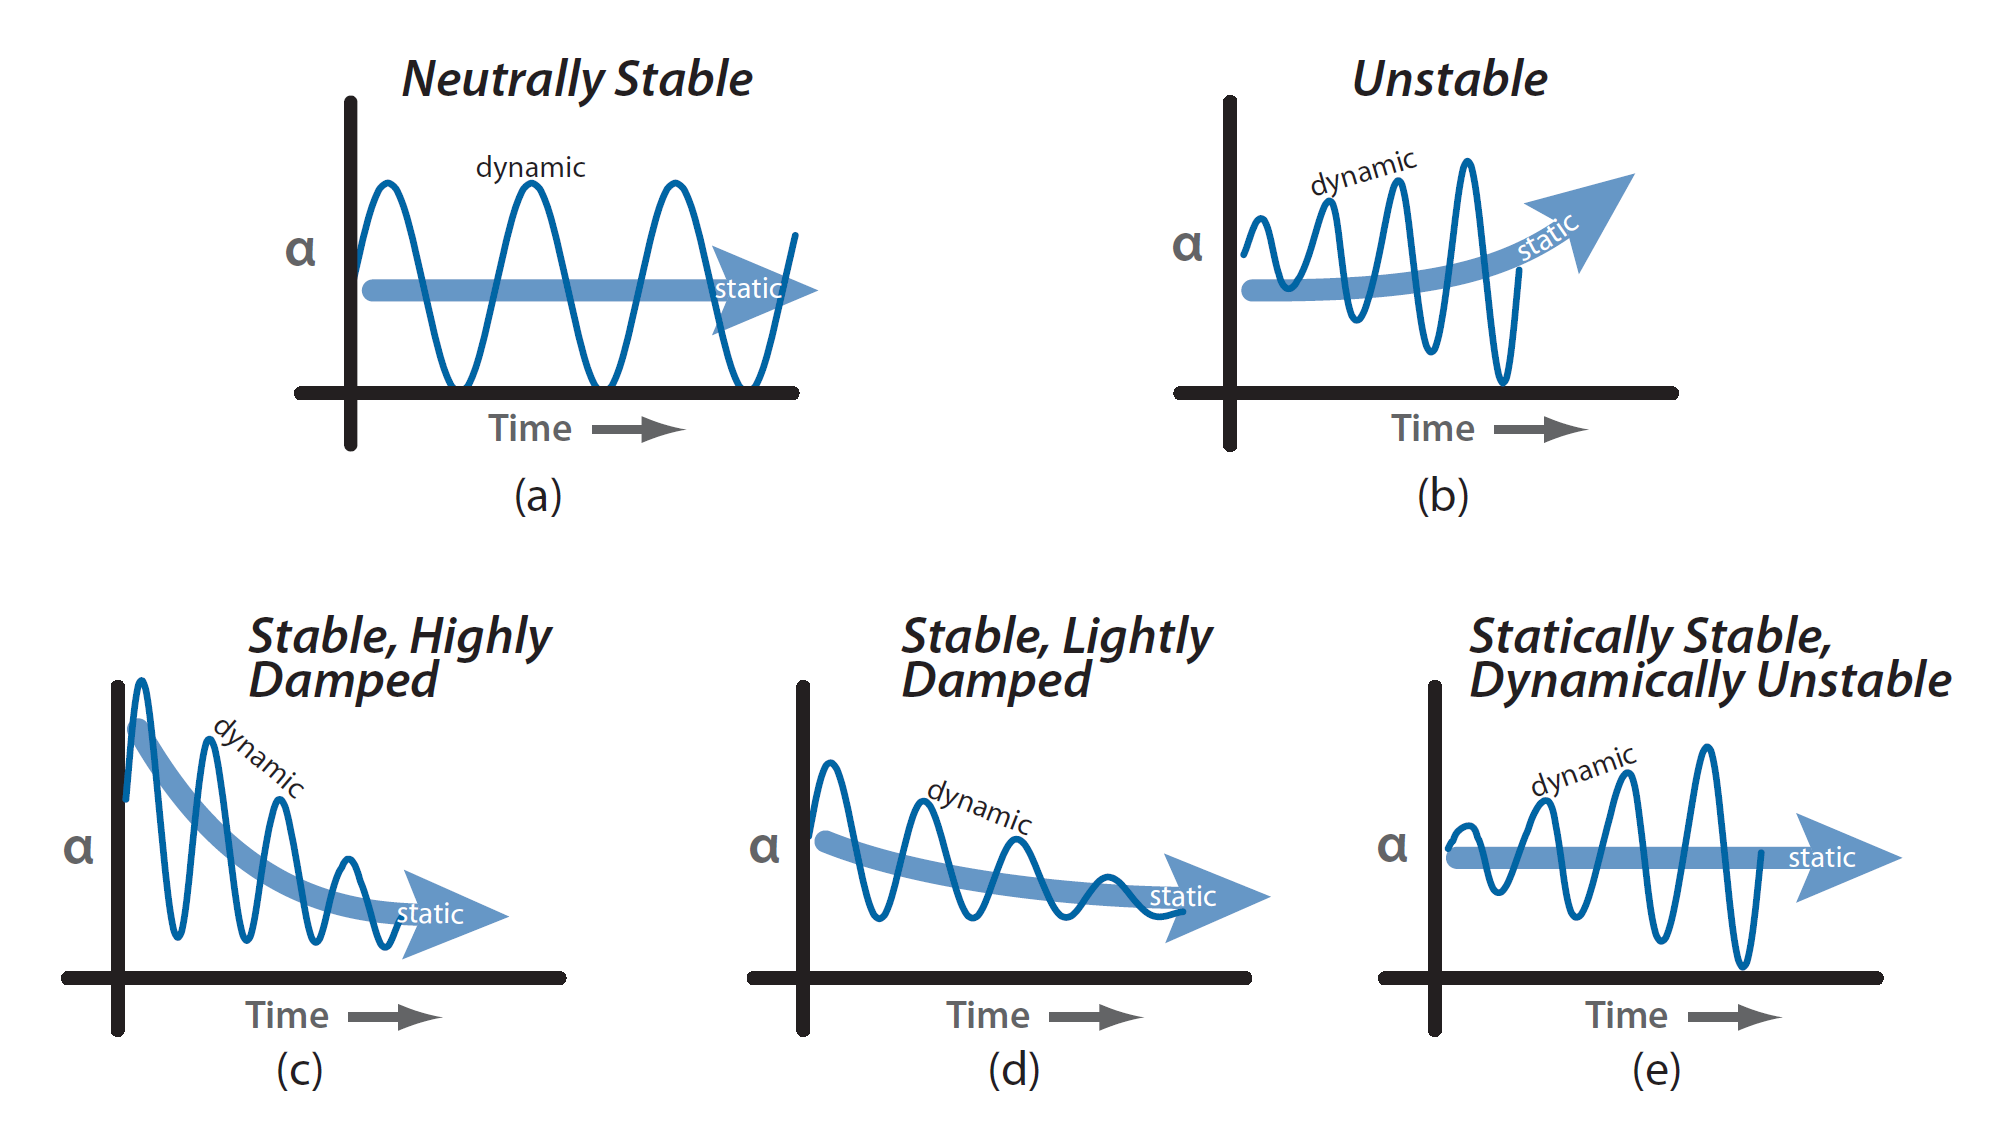
\includegraphics[height=8.6cm]{Immagini/stability}} 
\label{wblc}
\caption{Static and dynamic stability about the pitch axis.}
\end{figure} 		

It is important to note that there is a substantial difference between the concepts of ``Stability'' and ``Equilibrium''. In fact, stability is a characteristic of an aircraft, while equilibrium is a state in which airplane can be, that means the equilibrium of the forces and the moments acting on it.\\
``Longitudinal static stability'' is the stability of an aircraft in the longitudinal, or pitching, plane under steady-flight conditions. This characteristic is important because an airplane must have the tendency to return to the equilibrium position if perturbed. The pitch plane is the XZ plane of aircraft symmetry. The linear velocities are along the X-axis and w along the Z-axis. Angular velocity is about the Y-axis , known as pitching (positive if nose up). Pilot-induced activation of the elevator changes the aircraft pitch. In the plane of symmetry, the aircraft motion is uncoupled; that is, motion is limited only to the pitch plane.\cite{kundu}\\ \\
In order to evaluate the characteristics of longitudinal stability of an aircraft it's necessary to express all the forces and the moments acting on it and evaluate the resultant pitching moment about the center of gravity.\\
 The lift and drag are by definition always perpendicular and parallel to $V_{\infty}$. It is, therefore, inconvenient to use these forces to obtain moments because their moment arms relative to the center of gravity vary with angle-of-attack. For this reason, all forces are resolved into normal, N, and chord-wise, C, forces whose axes remain fixed with the aircraft and whose arms are, therefore, constant. \cite{nicolai2010fundamentals}\\

\begin{figure}[H]
\centering
{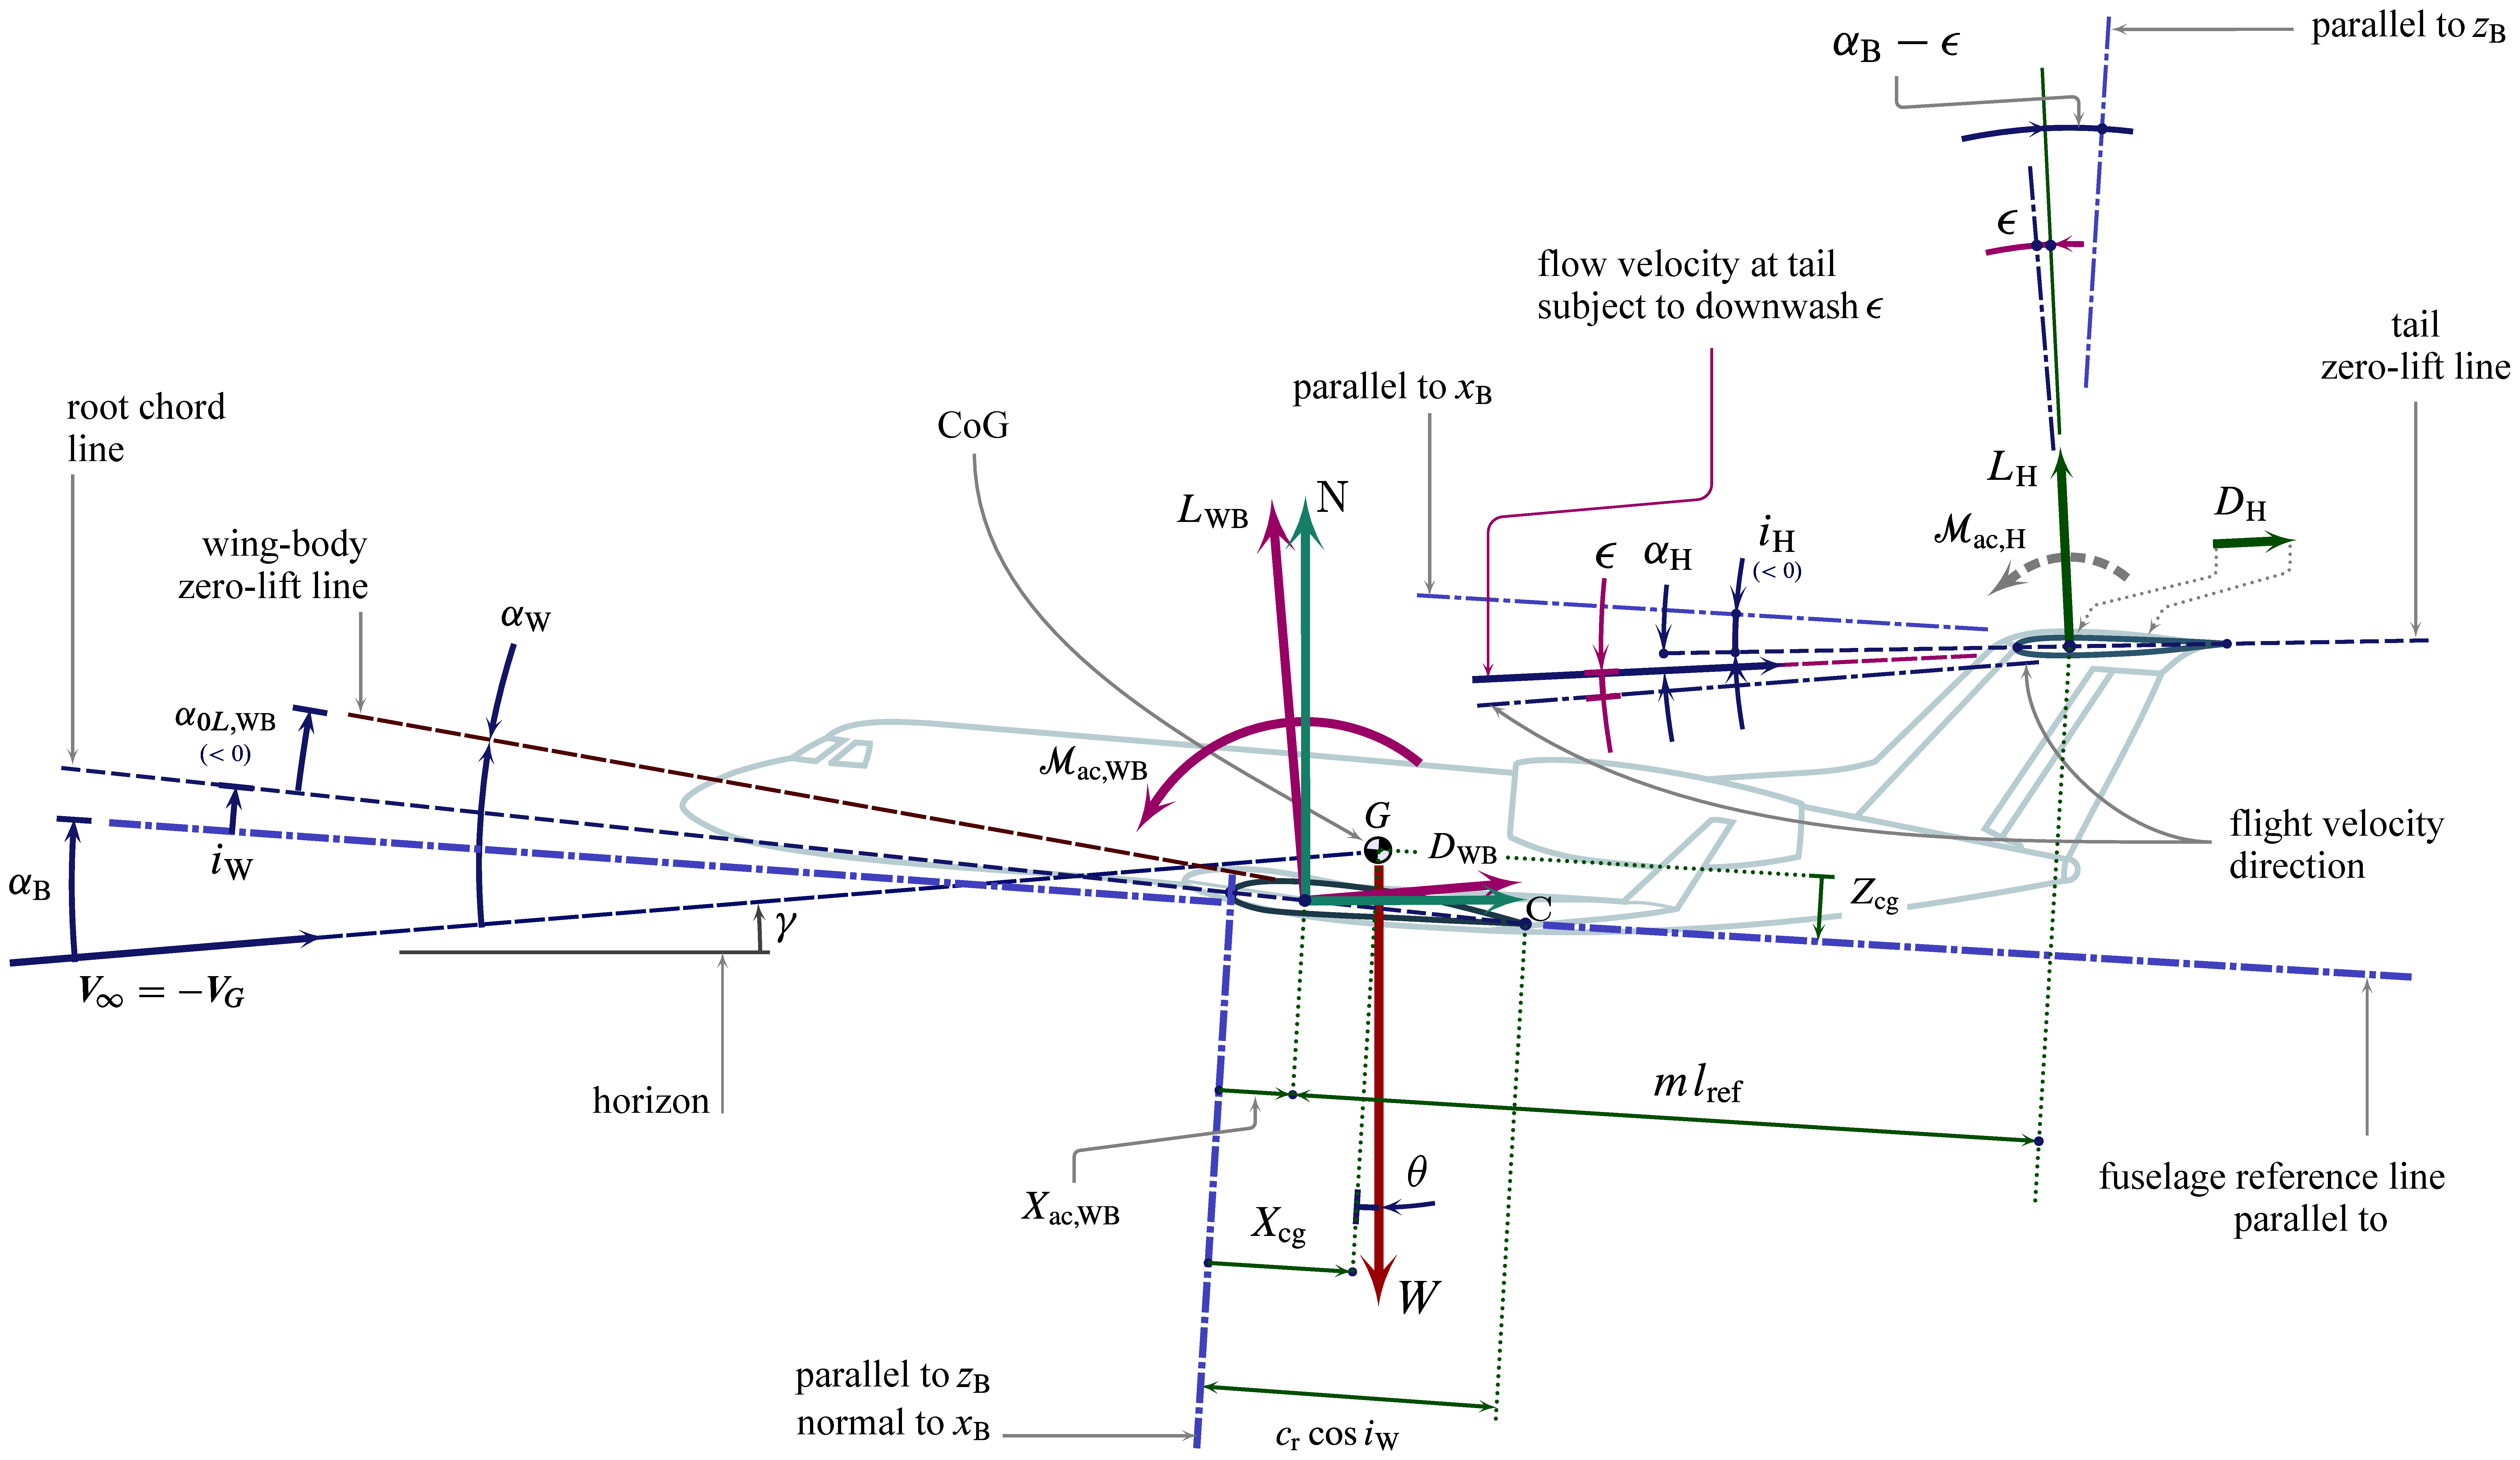
\includegraphics[height=9.4cm]{immagini/Longitudinal_Stability_Definitions_nc}} 
\label{longitudina}
\caption{Forces and moments acting on an aircraft..}
\end{figure} 	


The relation between the lift, the drag and the normal and chord-wise forces are the following:

\begin{equation}
N =L cos({\alpha}) + D sin({\alpha})
\end{equation}
\begin{equation}
C = D cos({\alpha}) - L sin({\alpha})
\end{equation}

According to what said, the aircraft can, in general, be trimmed, that is, put into an equilibrium state where the combined lift of the wing and the tail balances the weight while the moment about the center of gravity is zero. It's necessary that this equilibrium point corresponds to positive lift. As regards the stability it is necessary that the response of the aircraft to a disturbance in angle of attack is to tend to return to the original equilibrium position. Thus, if flying in equilibrium at one angle of attack and a disturbance increases the angle of attack, the moment produced at this angle of attack must act to reduce it, that is, tend back toward the original equilibrium state. Conversely, if a disturbance decreases the angle of attack, the moment at the new, lower, angle of attack must serve to increase that angle. \\
This means that the rate of change of the moment about the center of gravity must be negative for static stability: an increase in $\alpha$ should reduce $C_{M_{cg}}$ and a decrease in $\alpha$ should increase $C_{M_{cg}}$.\cite{sforza2014commercial} As higher is the   slope of the curve, greater is  the restoring moment. Thus the slope of the curve is called {\itshape Static Margin}.  Static margin is a concept used to characterize the static longitudinal stability and controllability of aircraft.
In aircraft analysis, static margin is defined as the distance between the center of gravity and the neutral point of the aircraft, expressed as a percentage of the mean aerodynamic chord of the wing.  In order to have static stability, thus, is necessary that the neutral point is behind the center of gravity.\\

In conclusion the requirements for static stability are the following:
\begin{itemize}
\item The pitching-moment curve exhibits a negative slope 
\item At a zero angle of attack there is positive nose-up moment
\end{itemize}

\begin{figure}[H]
\centering
{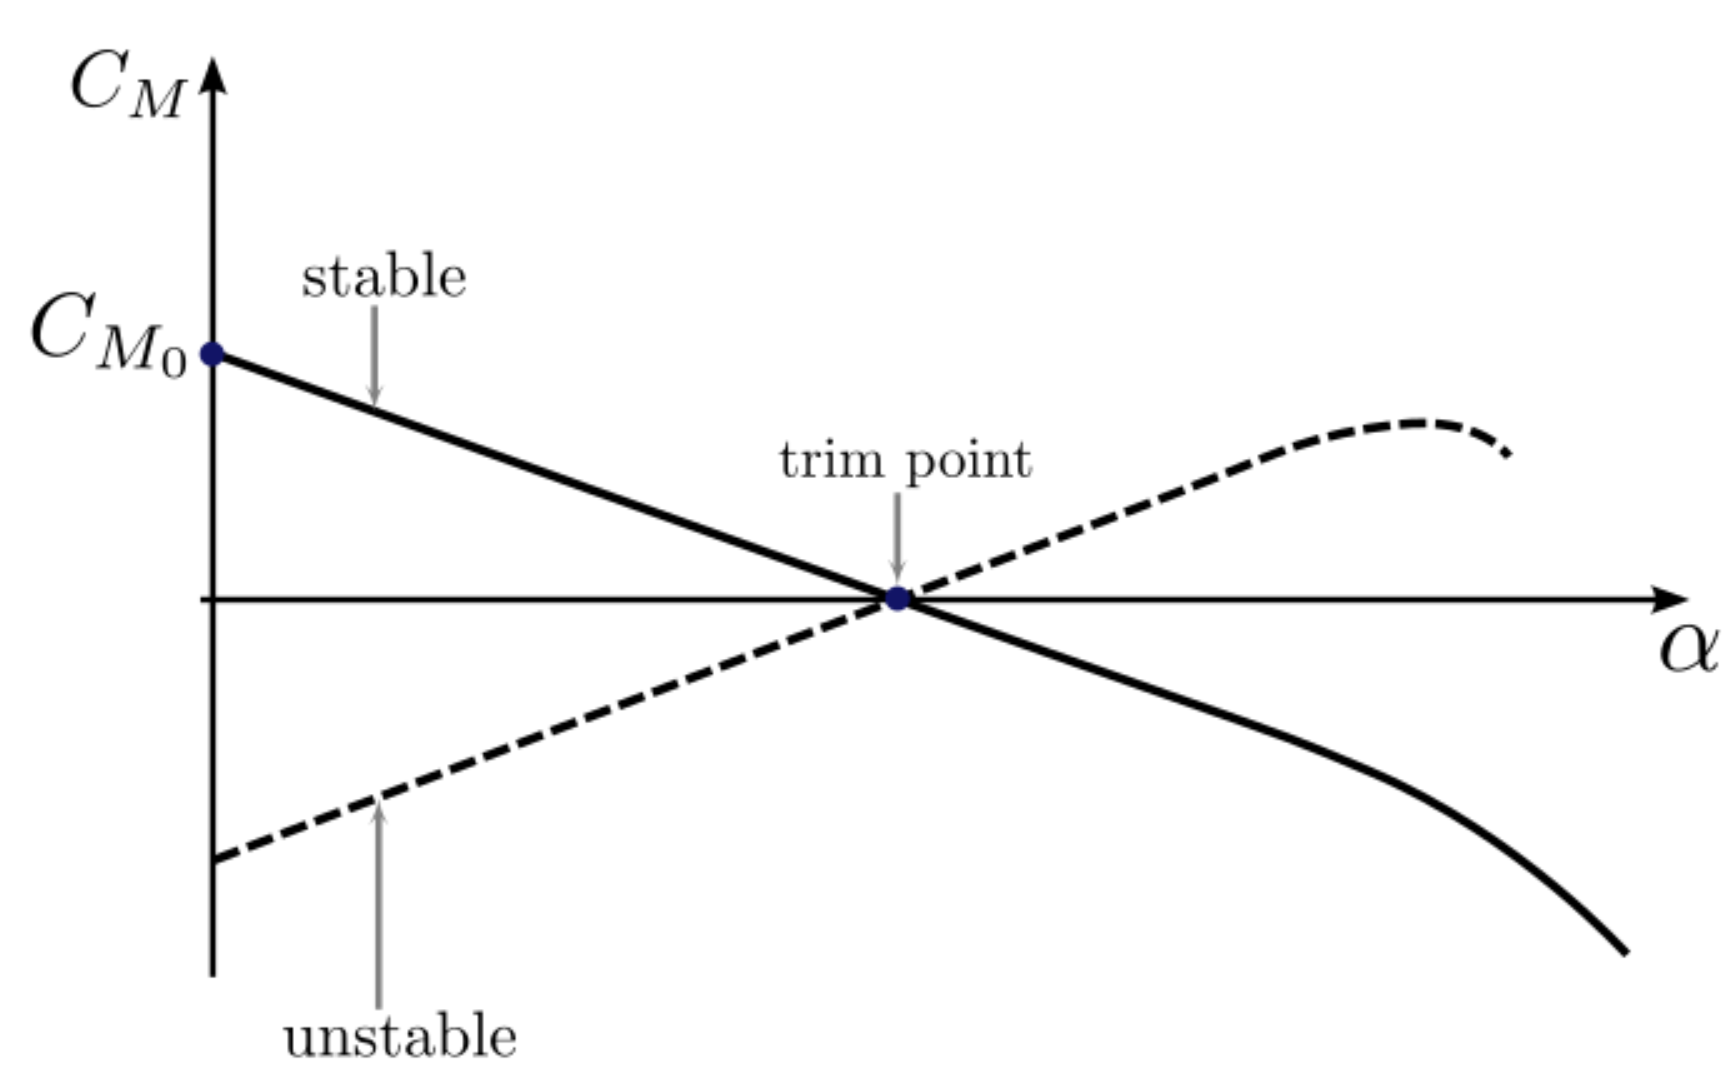
\includegraphics[height=6cm]{immagini/cm}} 
\label{stabinstab}
\caption{Qualitative representation of the moment coefficient vs $\alpha$.}
\end{figure} 	


Below will be calculated all the contributions in order to evaluate the pitching moment coefficient about the center of gravity. 

% scopo del piano di coda--> garantire equilibrio a diversi angoli.. sforza

% introduzione... stabilità, grafici e quali sono tutti i dati che servono
%Nicolai 585 
%Sforza 250
%kundu 387
%disegno stabilità
\section{Aerodynamic Lift}		
 Considering a reference angle of attack $\alpha_B$, the aircraft components generates lift. So it is necessary to evaluate these contributes. In particular, first of all, is wanted to evaluate the $C_L$ of isolated wing. This value will be correct with fuselage influence. Afterwards it is necessary to evaluate the contribute of horizontal tail.  It is important to note that each component works at a different angle of attack in dependence of angles of incidence and downwash , meanwhile for longitudinal stability the reference angle of attack is $\alpha_B$.

\subsection{Wing}
 The wing may be considered as the most important component of an aircraft. Its main purpose is  to generate sufficient lift force. However, the wing has two other productions, namely drag force or drag and pitching moment. While a wing designer is looking to maximize the lift, the other two (drag and pitching moment) must be minimized. \\
 The theoretical background and the followed process are shown in the CHAPT \ref{ch:worklift}.

\subsection{Fuselage}

The fuselage is that portion of the aircraft wherein the payload is carried. In jet transports the payload consists of the passengers and their baggage and/or cargo. It is important that the fuselage has some features as a low aerodynamic drag; a minimum aerodynamic instability;  comfort and attractiveness in terms of seat design, placement, and storage space; safety during emergencies; minimization of noise and ease of cargo handling in loading and unloading.\cite{sforza2014commercial} \\ \\ 


The lift distribution on a wing is affected by the presence of the fuselage as a result of the following effects:
\begin{itemize}
\item The presence of the fuselage disturbs the longitudinal velocity field near the wing.
\item At an angle of attack relative to the free stream, the fuselage also perturbs the flow about the wing in planes normal to the free stream.
\item The fuselage has a blocking effect on the flow.
\end{itemize}

\begin{figure}[H]
\centering
{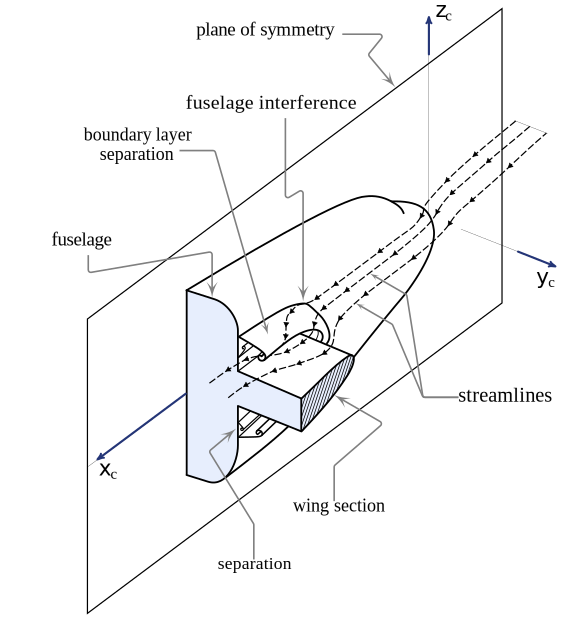
\includegraphics[height=11cm]{Immagini/wf}} 
\label{wf}
\caption{Wing fuselage junction flow.}
\end{figure} 		



These effects are not large for a slender fuselage but may be important when the fuselage is relatively bulky, so that a substantial alteration to the local longitudinal velocity may result. The cross-flow caused by the fuselage at angle of attack changes the component of free stream velocity normal to the fuselage axis and affects the downwash flow produced by the wing. The blocking effect of the fuselage is always present even if the fuselage is an infinite cylinder aligned with the free stream, in which case the other two effects are not present. \cite{sforza2014commercial}

\begin{figure}[H]
\centering
{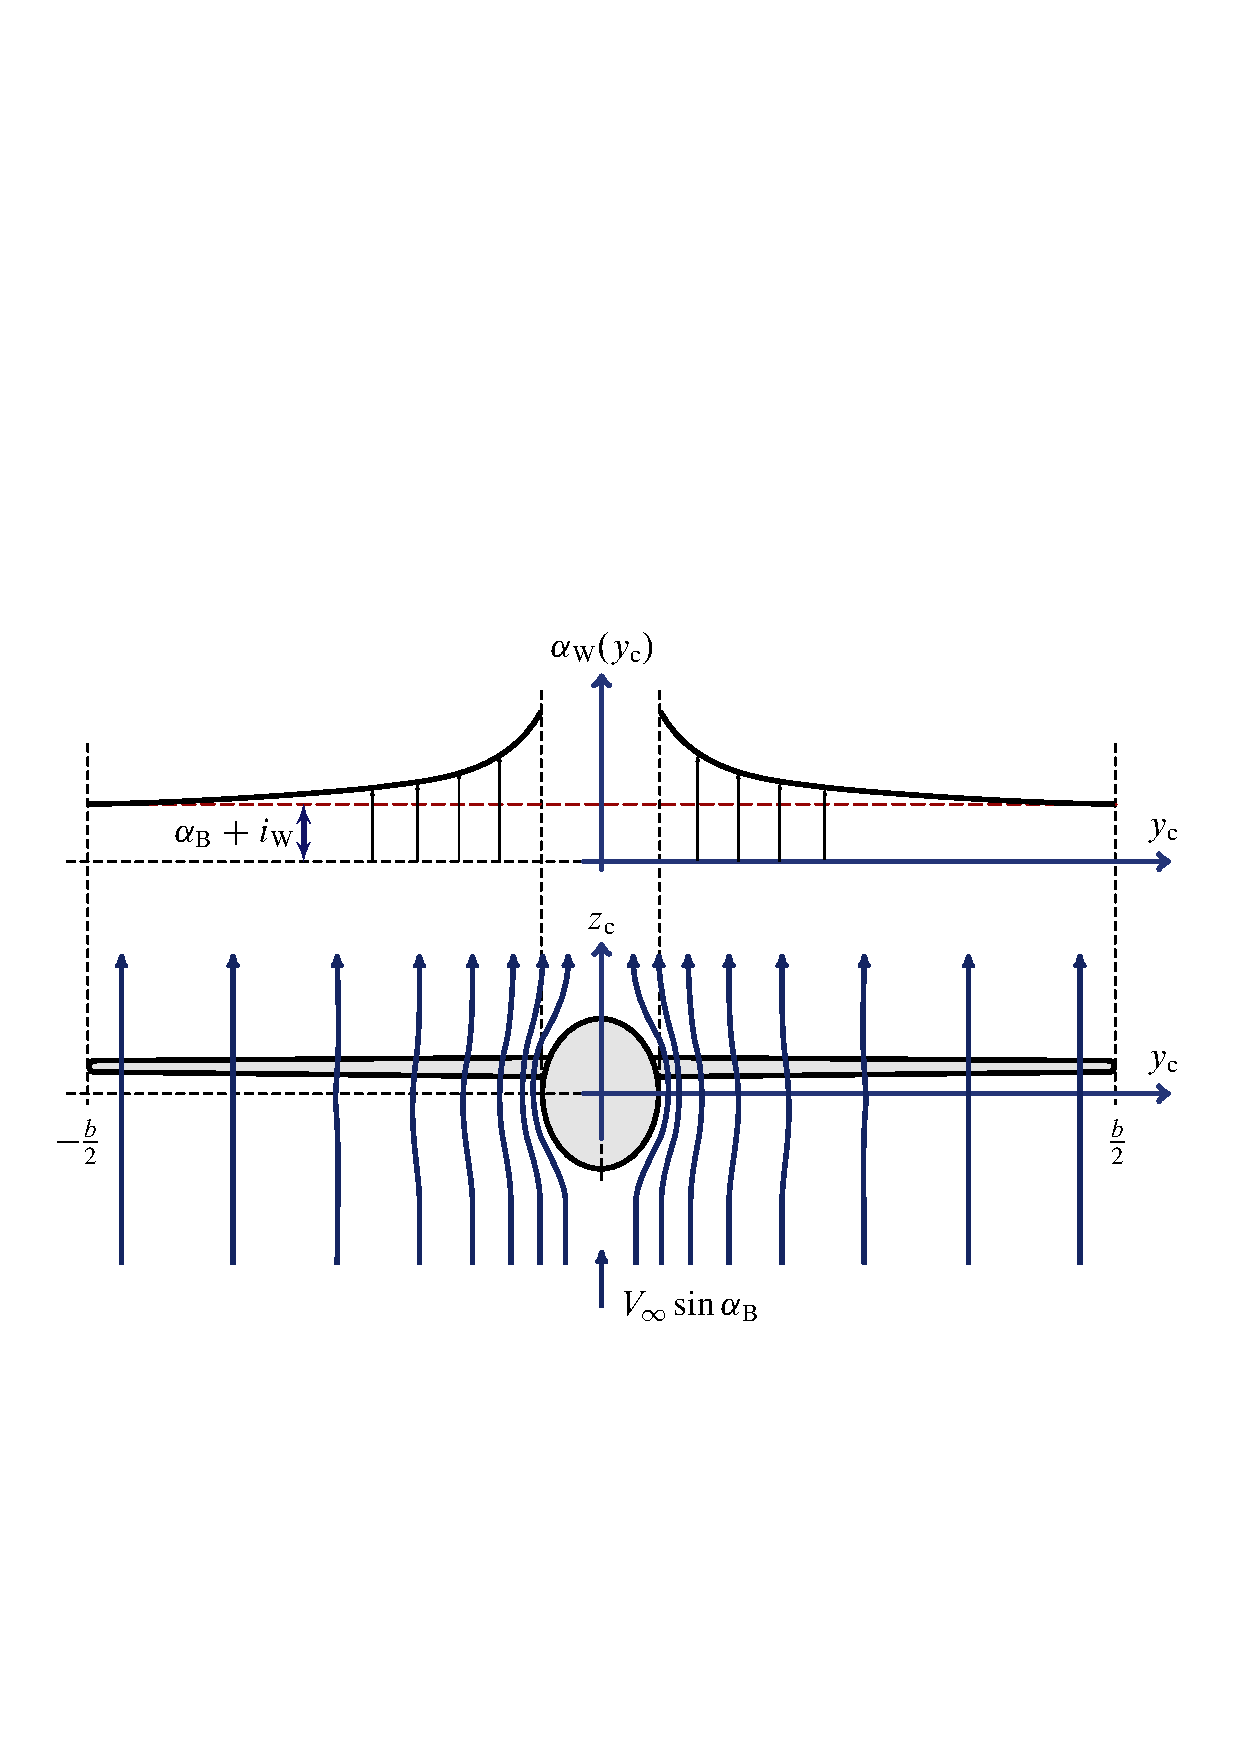
\includegraphics[height=8.63cm]{Immagini/wing_fuselage_front_view_interference.pdf}} 
i\label{wf2}
\caption{Wing fuselage front view interference.}
\end{figure} 		




However, theoretical analysis showed that the presence of a slender fuselage does not have an important effect on the lift
distribution on an unswept wing of moderate aspect ratio, but a larger change in the lift distribution on a wing in the presence of a fuselage may be anticipated if the wing is swept.\cite{zlotnick}
For greater accuracy of the calculation, the value of lift linear slope has been corrected using the following equation from \cite{roskammethods}:

\begin{equation}
\left ( \frac{d C_L}{d\alpha} \right)_{w \!b} = \left[ 1 + \frac{1}{4} \left ( \frac {d}{b} \right ) - \frac{1}{40} \left (\frac{d}{b} \right) ^2 \right] \left ( \frac{d C_L}{d\alpha} \right)_{w}
\end{equation}

\noindent  \\ \\
Note that for typical airliners $\frac{d}{b} \approx 0.1$ and therefore the lift curve slope of the wing-body is approximately equal to that of the wing alone.\\
In addition to the calculation of the linear slope of the wing body group, it is necessary to calculate the intersection point between the lift curve of wing and the lift curve of wing-body. This point is the $\alpha_{0_L}$ of the exposed wing. The exposed wing is the part of wing outside of the fuselage that generates lift in a complete aircraft. This value has been calculated with the following integral formula.

\begin{equation}
\alpha_{0L} |_{EW} = \frac{2}{S_E}\int_{y_{0_E}}^{\frac{b}{2}} c(y) [ \alpha_0(y_E) - \epsilon_T(y_E) ] \, dy
\end{equation}


\begin{figure}[H]
\centering
{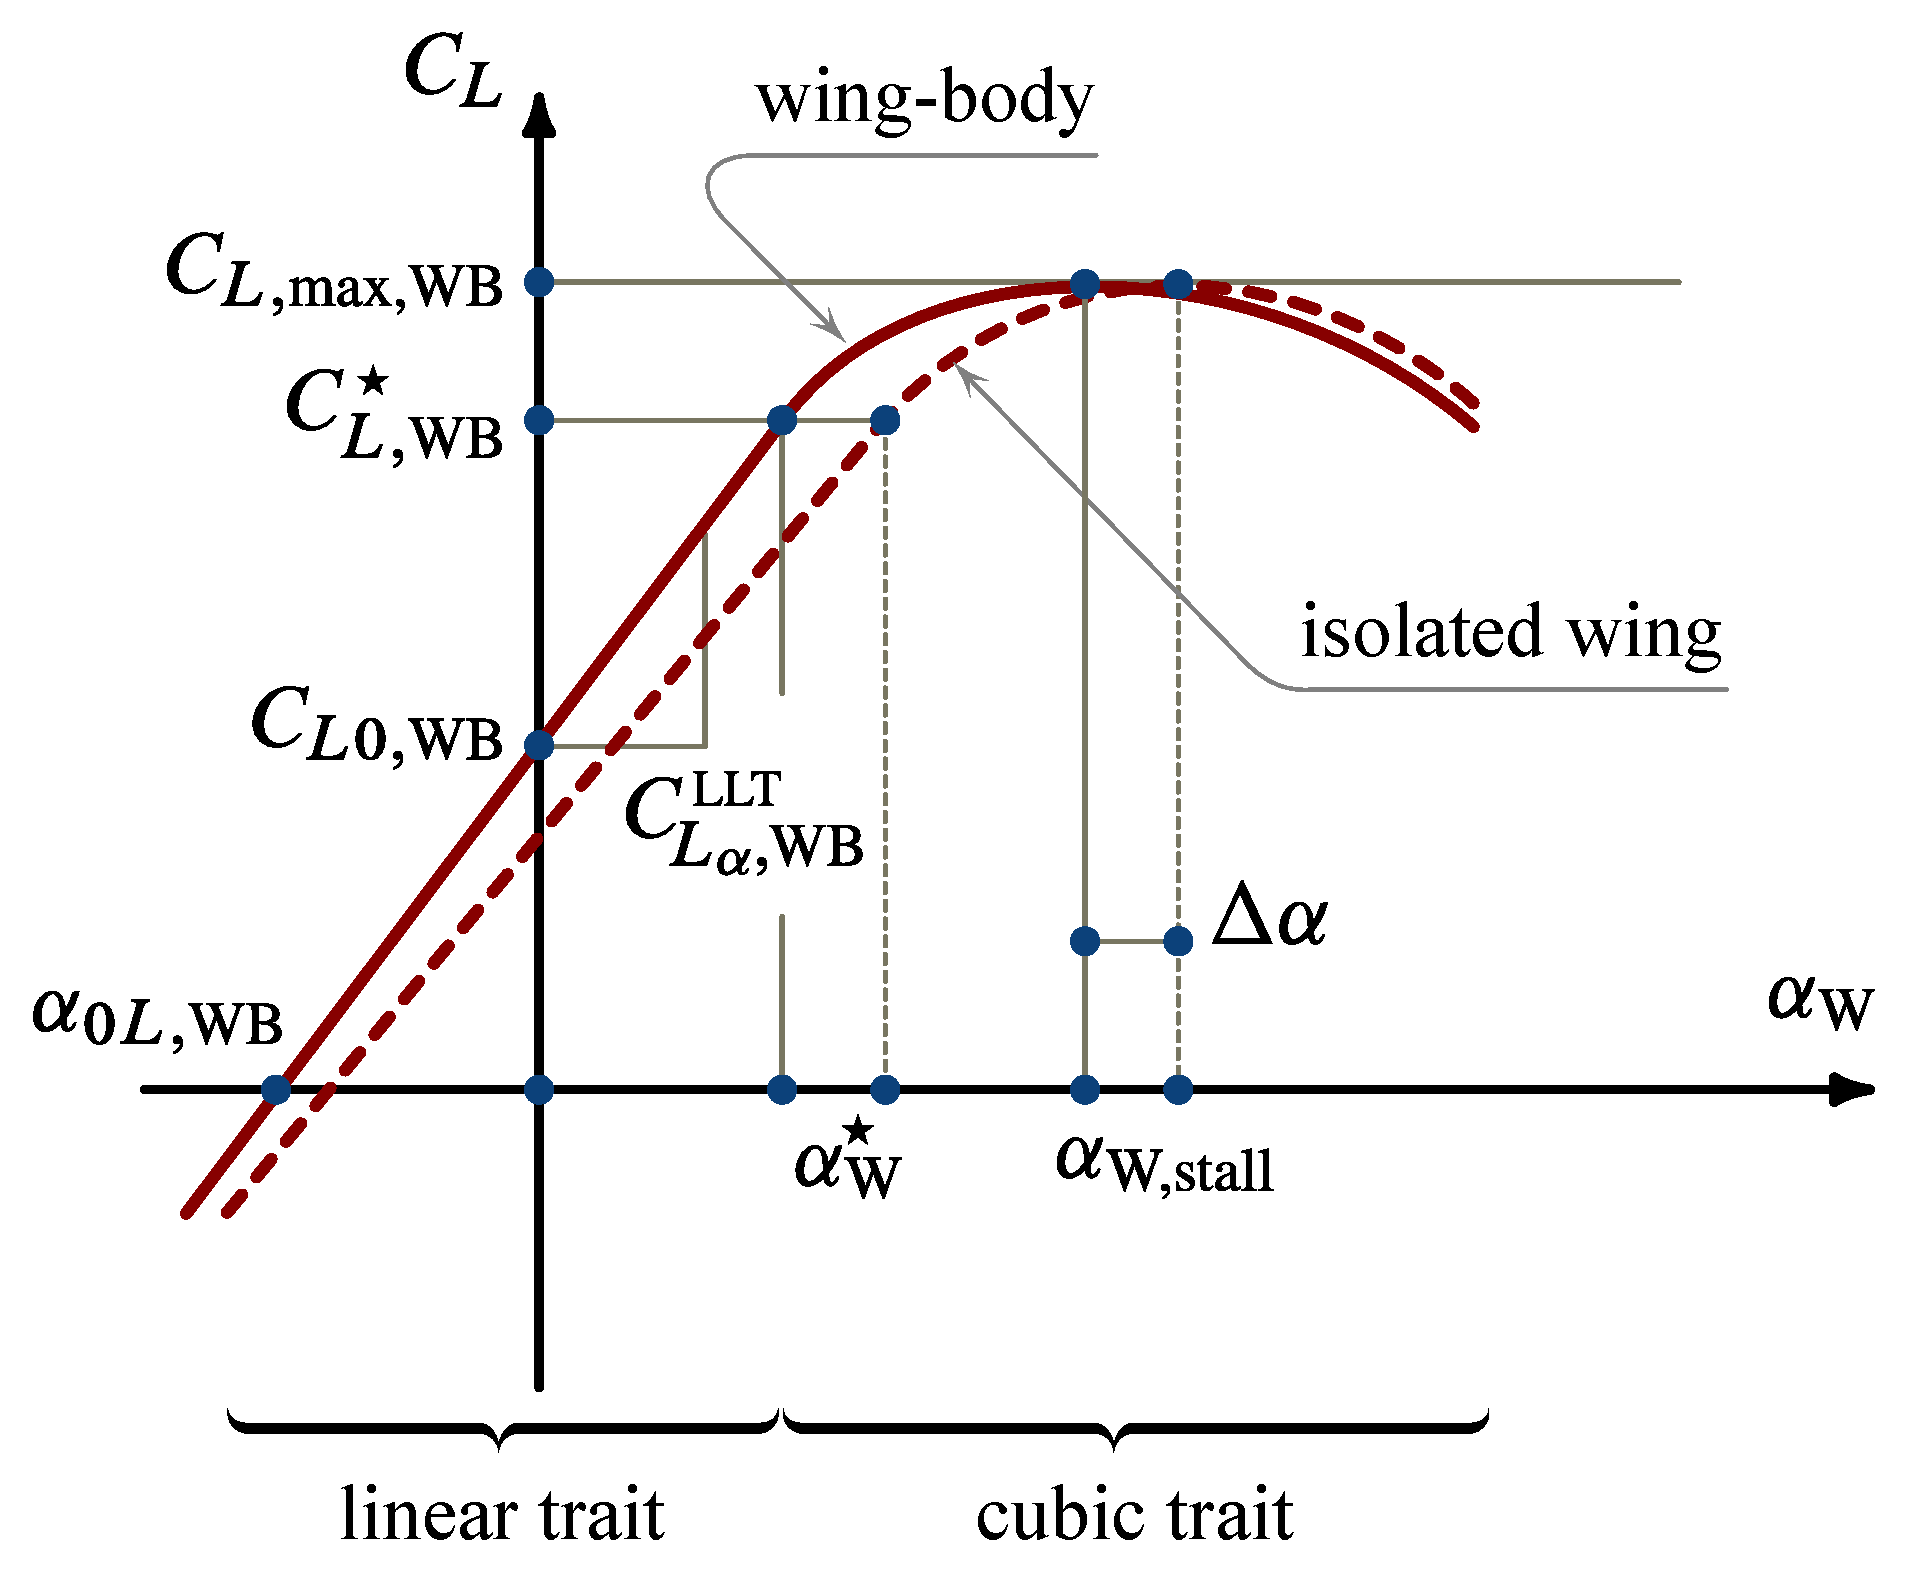
\includegraphics[height=8.9cm]{Immagini/WingBody_CL_Vs_alpha_curve}} 
\label{wblc}
\caption{Lift curve of isolated wing and of wing-body group.}
\end{figure} 		


\subsection{Horizontal Tail}

The horizontal tail  is an aerodynamic surface, typically including one or more movable control surfaces,that provides longitudinal stability and control. A stabilizer can feature a fixed or adjustable structure on which any movable control surfaces are hinged, or it can itself be a fully movable surface. In the first case the horizontal tail consists of the {\itshape stabilizer} and the  {\itshape elevator} (moving) for handling the pitch degree of freedom. In case of a fully movable surface it is called  {\itshape stabilator}. \\
 The H-tail can be positioned low through the fuselage, in the middle cutting through the V-tail, or at the top of the V-tail to form a T-tail. \cite{kundu}
The horizontal tail provides longitudinal stability and control. It may be sized by one or more of the following conditions\cite{obert2009aerodynamic}:

\begin{itemize}
\item Provide static and dynamic stability.
Provide a state of equilibrium in each flight condition.
\item Enable aircraft control.
\item Provide a state of equilibrium in each flight condition.
\end{itemize}

The stabilizer is a fixed wing section whose job is to provide stability for the aircraft, to keep it flying straight. The horizontal stabilizer prevents up-and-down, or pitching, motion of the aircraft nose. The elevator is the small moving section at the rear of the stabilizer that is attached to the fixed sections by hinges. Because the elevator moves, it varies the amount of force generated by the tail surface and is used to generate and control the pitching motion of the aircraft. There is an elevator attached to each side of the fuselage. The elevators work in pairs; when the right elevator goes up, the left elevator also goes up.

Considering an horizontal tail formed by stabilizer and elevator, in order to evaluate the lift coefficient of this lifting surface it is necessary to consider the deflection of control surface. The elevator, in fact, can be considered as a {\itshape plain flap}.

\subsubsection{Elevator index of effectiveness}
 In order to evaluate the contribution to the longitudinal stability of horizontal tail it's necessary to consider the deflection of the elevator. 
		
\begin{figure}[H]
\centering
{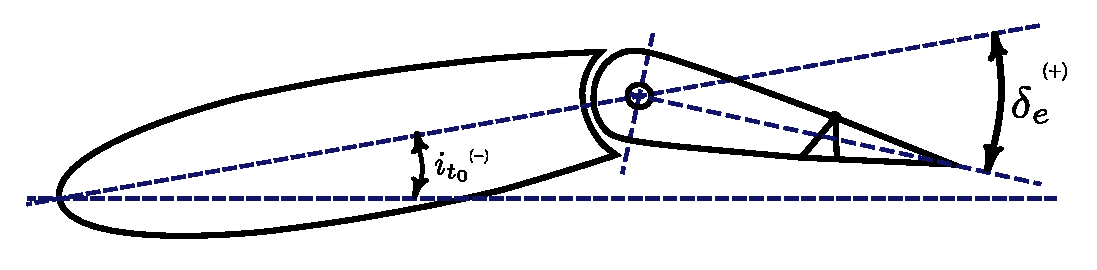
\includegraphics[height=2.3cm]{Immagini/horizontal_tail_profile_deltaE.pdf}} 
\label{htailangle}
\caption{Characteristic angles of the horizontal tail.}
\end{figure} 		
		
The variation of zero lift angle is not constant with the angle of deflection. So it's necessary to evaluate the tau factor which is defined as follows:

\begin{equation}		 
\tau_e = \frac{d \alpha_{0l}}{d \delta_e}
\end{equation}

		
Introducing this parameter the lift coefficient of the horizontal tail can be rated as follows:

\begin{equation}
C_{L_H}= C_{L_0} + C_{L_{{\alpha}_H}} \alpha_H + 	C_{L_{{\alpha}_H}} \tau_e \delta_e
\end{equation}

  
Considering a symmetrical horizontal tail, the term $C_{L_0}$ is zero, so it's possible to express the lift coefficient in the following form:


\begin{equation}
C_{L_H}= C_{L_{{\alpha}_H}} \left ( \alpha_H + \tau_e \delta_e \right)
\end{equation}
  		
 In general the value of $\tau$ is constant until about 15 deg; after this value, due to the flow separation, the effectiveness of elevator decrease and consequently the product $ \tau_e \delta_e$ that appears in the equation of lift coefficient.
		


%
%\begin{figure}[H]
%\centering
%{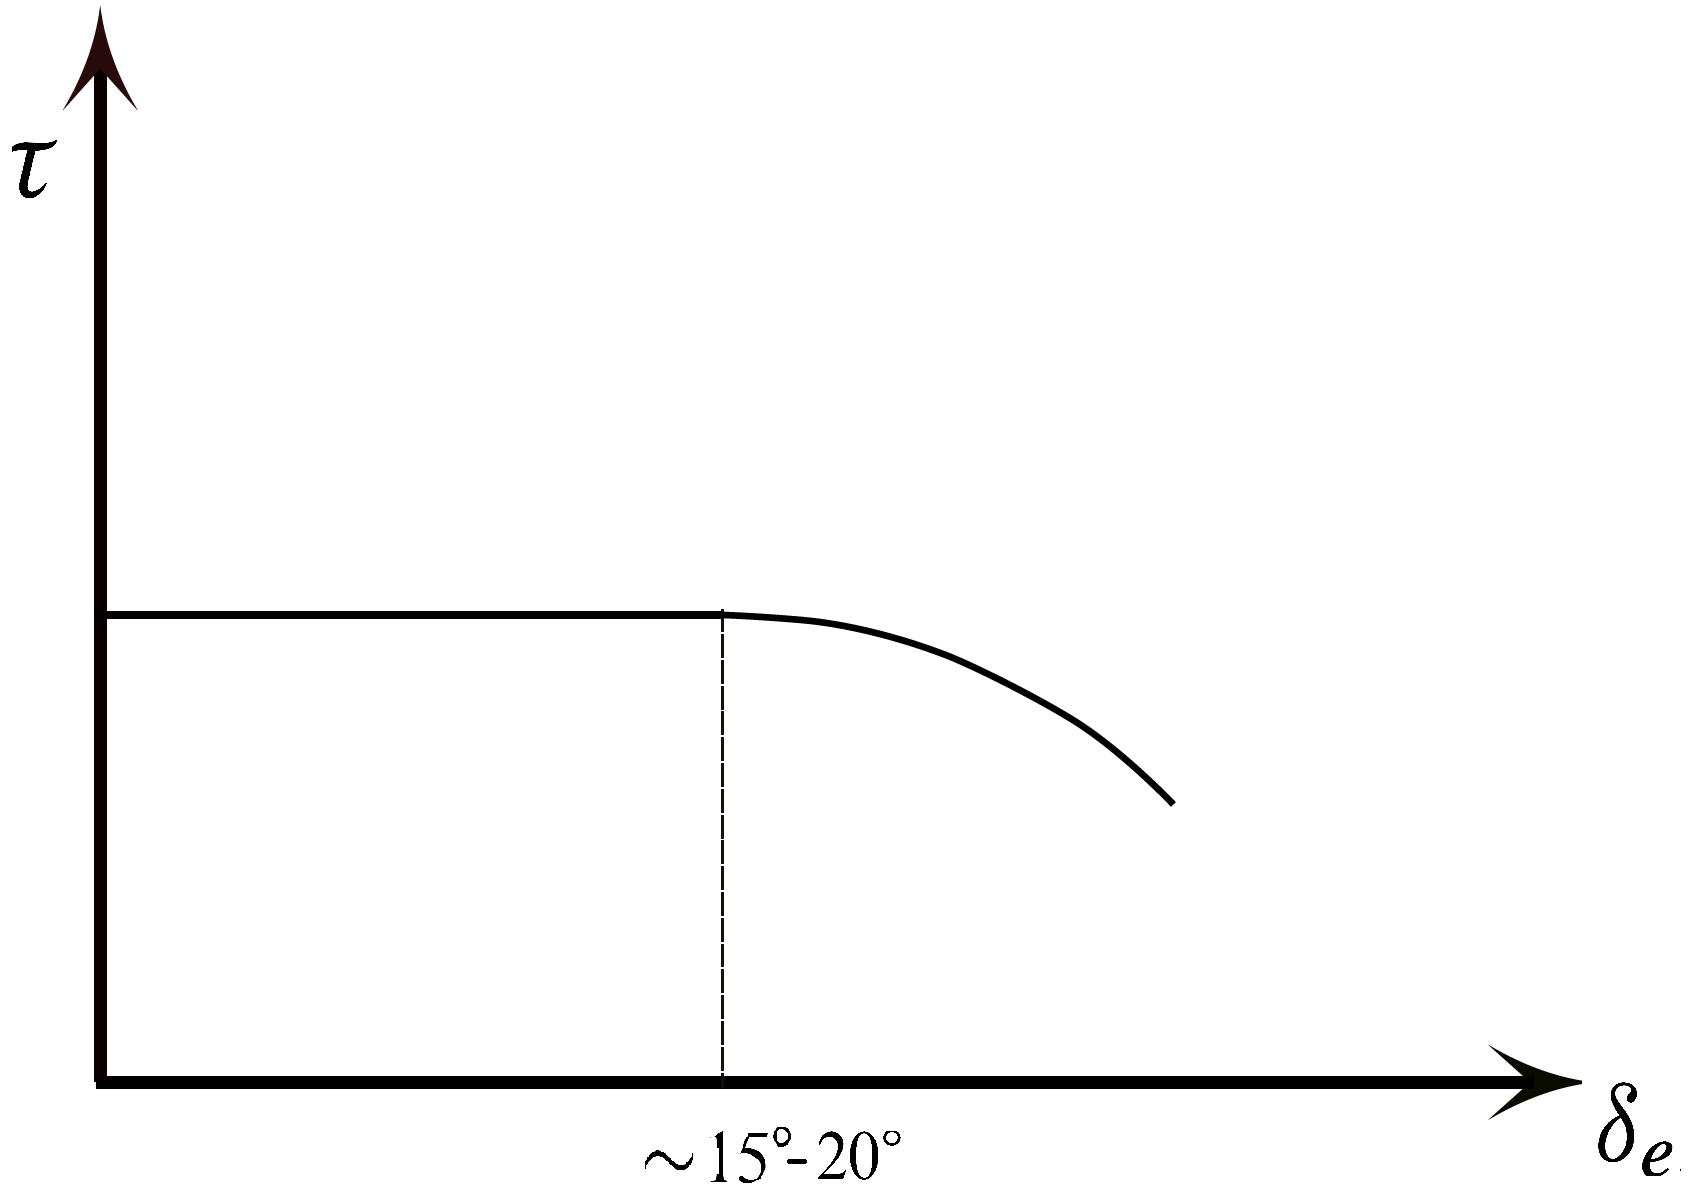
\includegraphics[height=6.79cm]{Immagini/taude.png}} 
%\label{tau1}
%\caption{Qualitative trend of $\tau$ with the deflection of elevator.}
%\end{figure} 		
%
%
%\begin{figure}[H]
%\centering
%{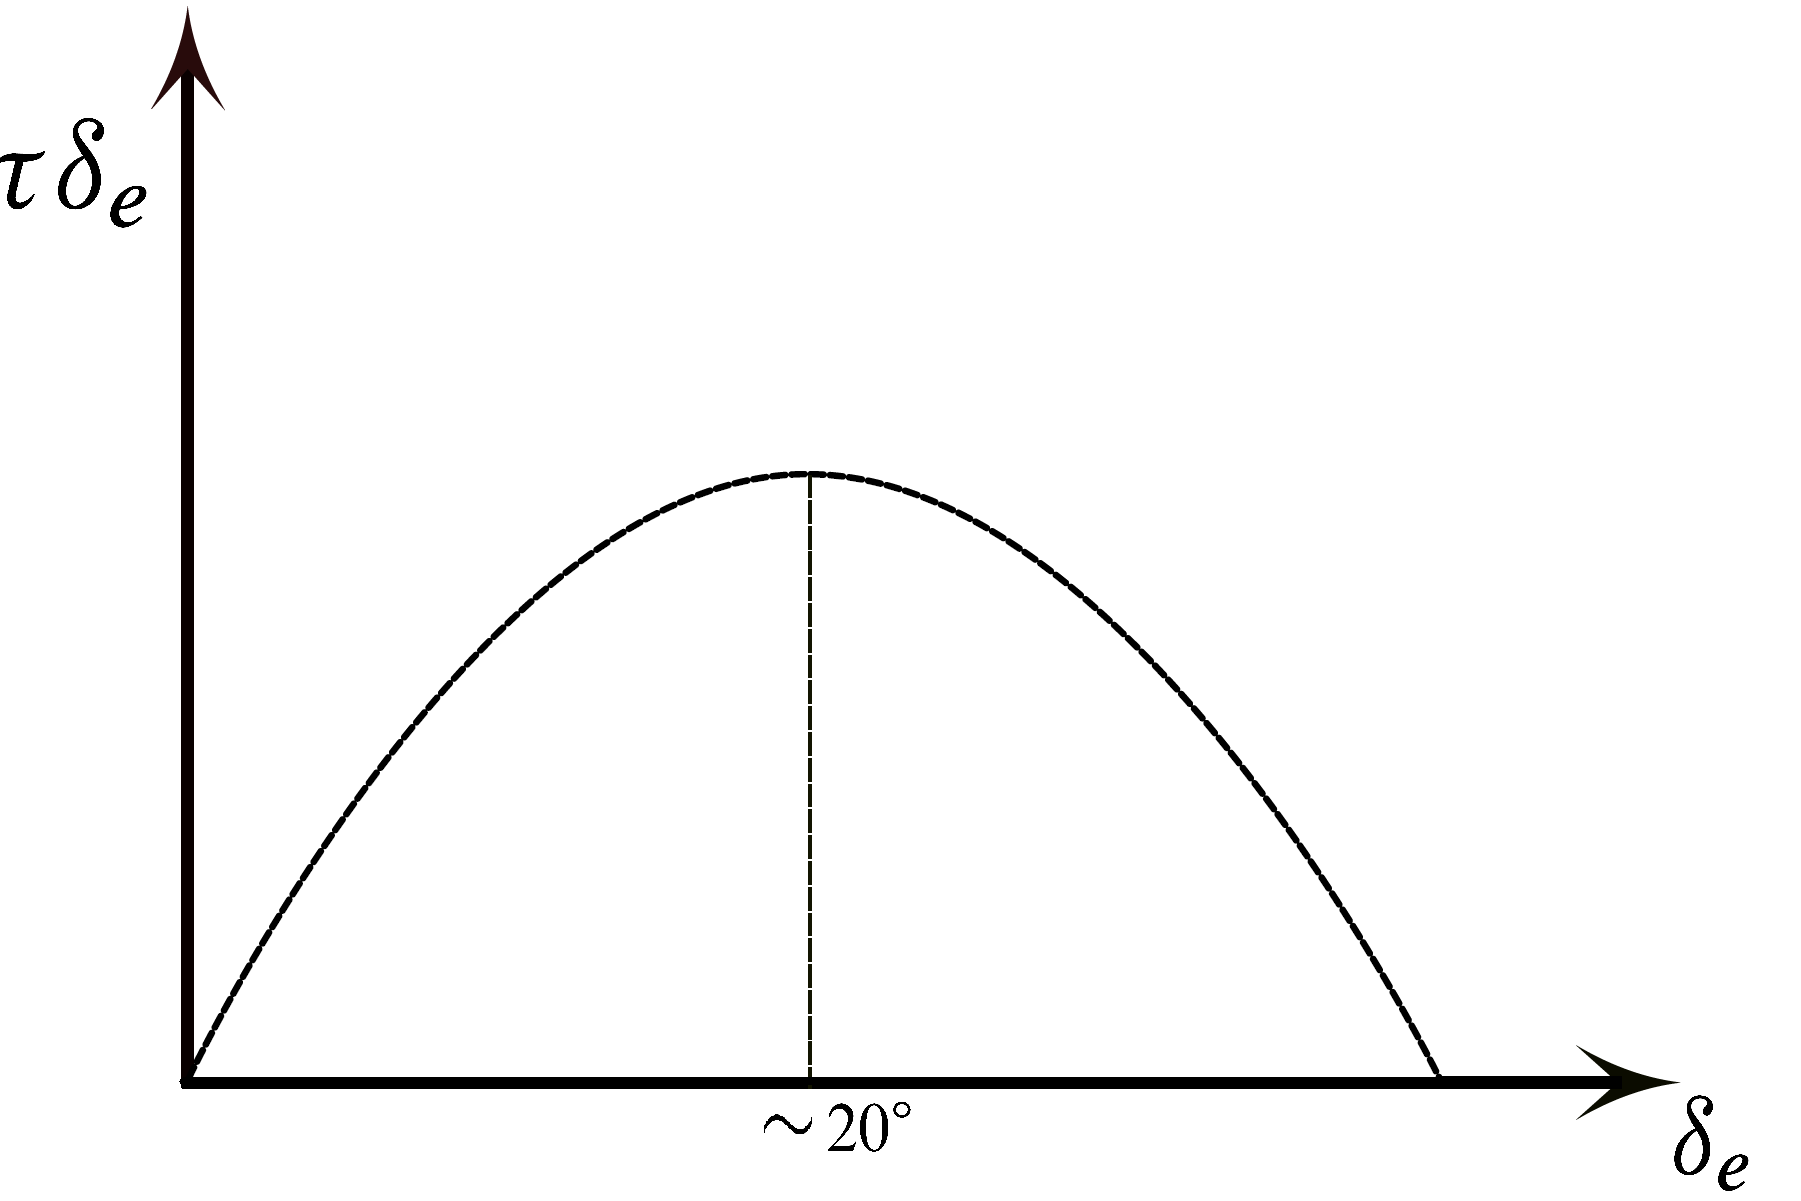
\includegraphics[height=6.79cm]{Immagini/taudeltae.png}} 
%\label{tau2}
%\caption{Qualitative trend of the term $\tau \cdot \delta_e$ with the deflection of elevator.}
%\end{figure} 		

\begin{figure}[H]
\centering
\begin{minipage}{.5\textwidth}
\centering
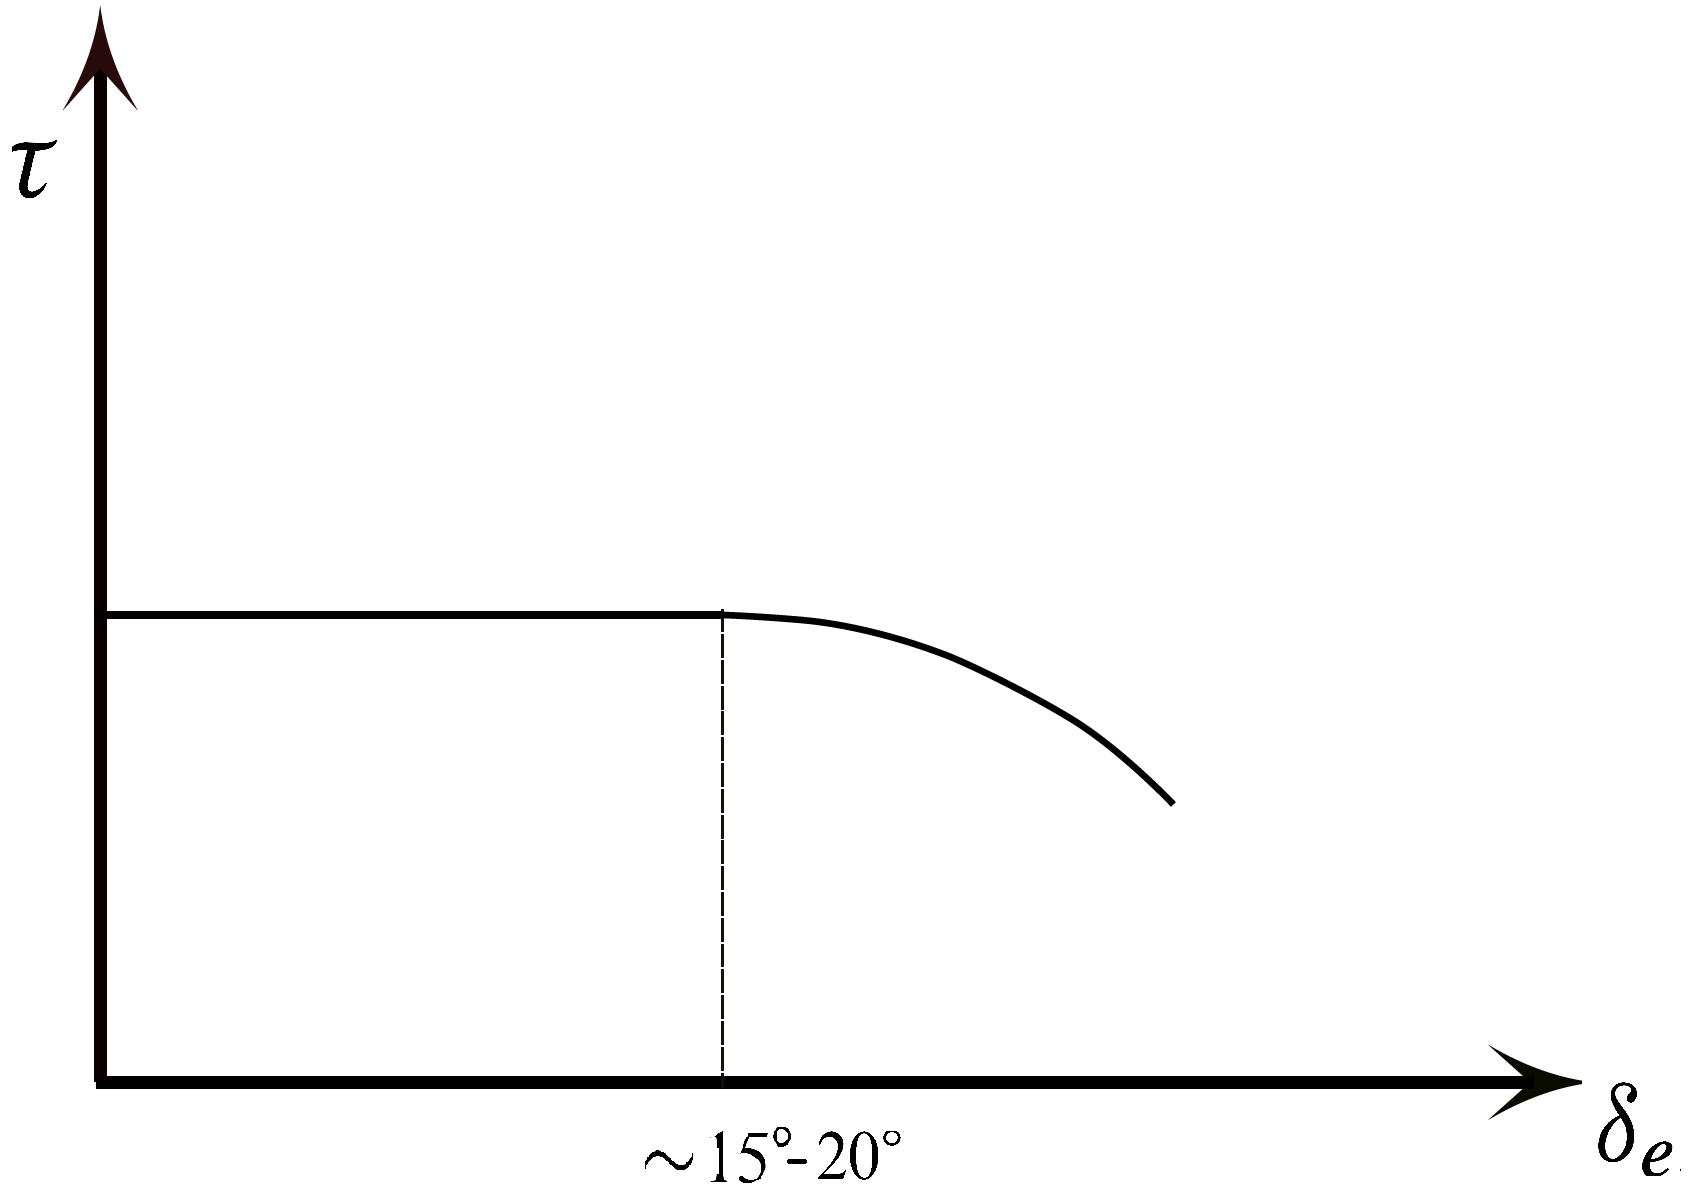
\includegraphics[height=5.3cm]{Immagini/taude.png}
\captionof{figure}{Qualitative trend of $\tau$ with  \\ the deflection of elevator.}
\label{tau1}
\end{minipage}%
\begin{minipage}{.5\textwidth}
\centering
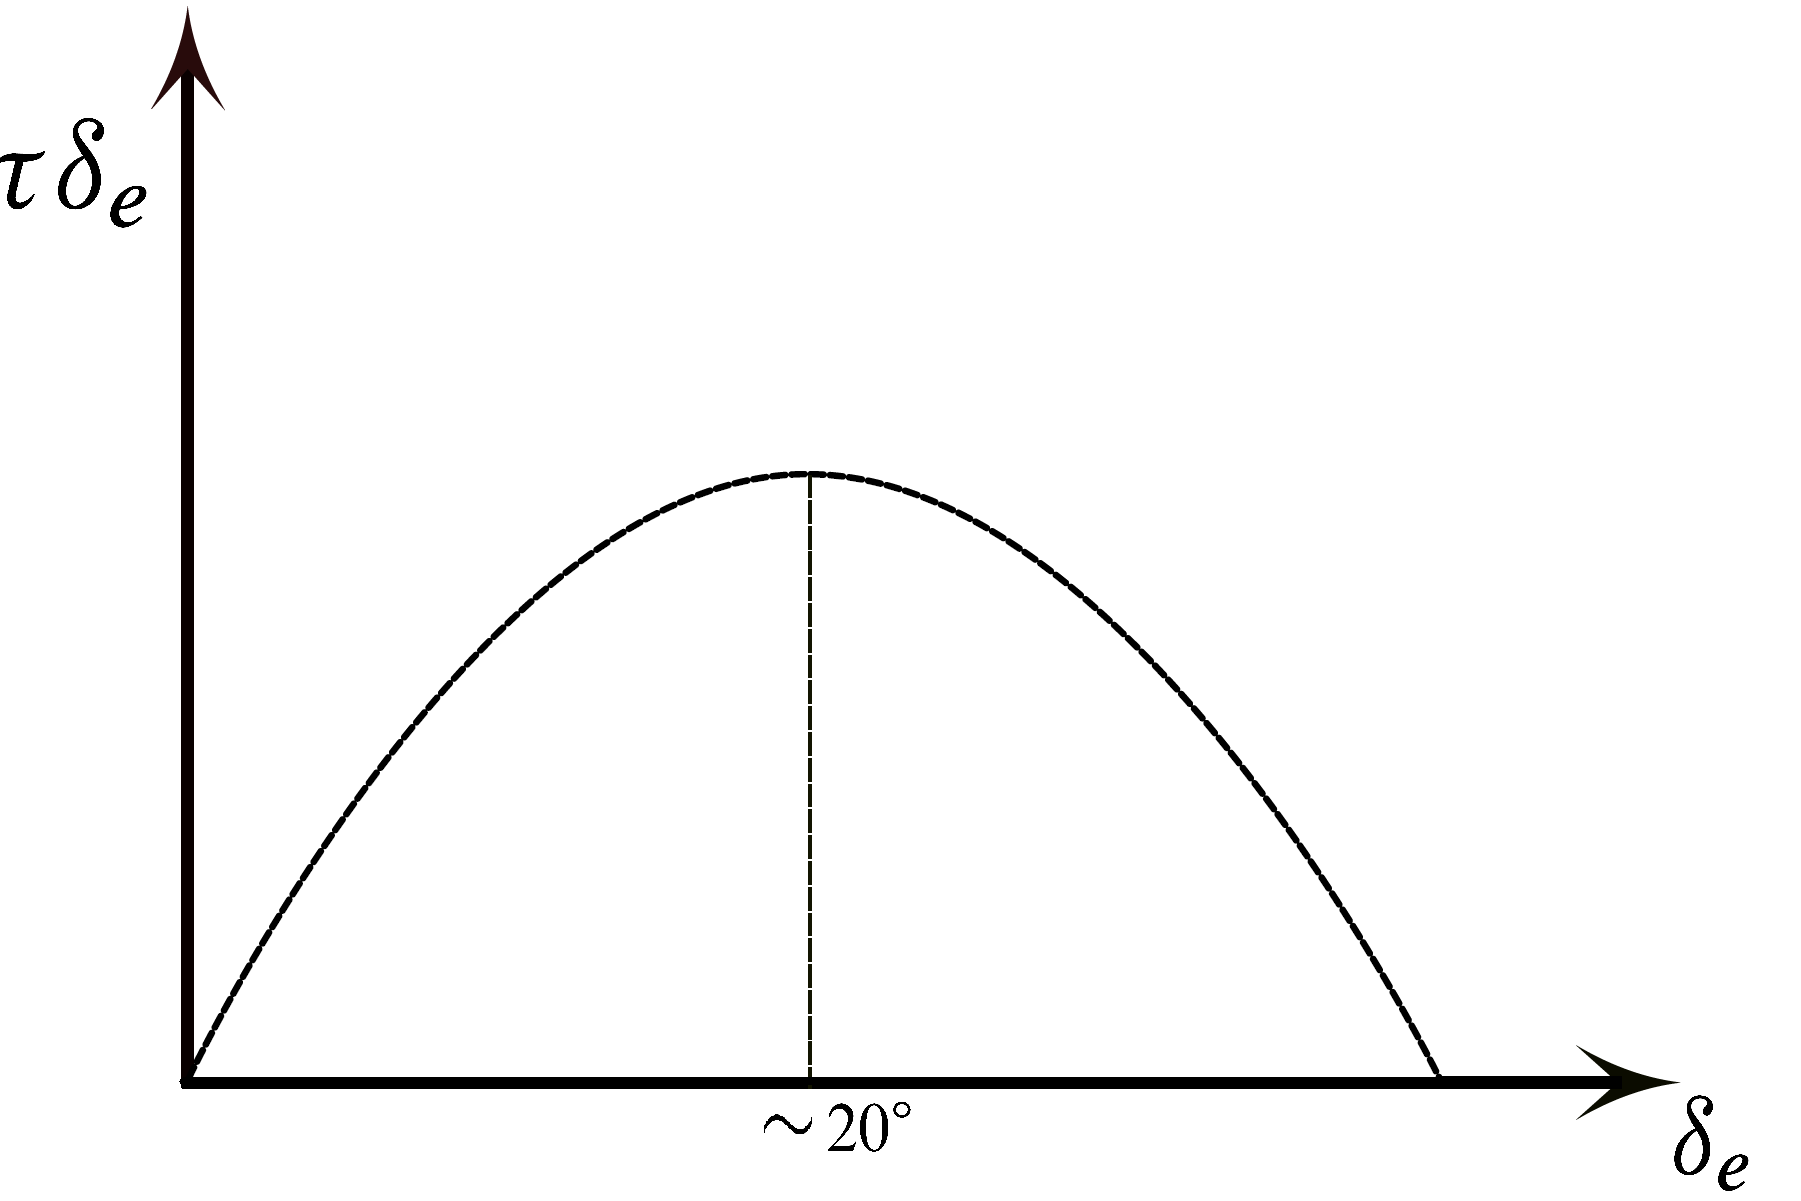
\includegraphics[height=5.3cm]{Immagini/taudeltae.png}
\captionof{figure}{Qualitative trend of the term $\tau \cdot \delta_e$ with the deflection of elevator.}
\label{tau2}
\end{minipage}
\label{fig:effects}
\end{figure}


%\begin{figure}[H]
%\centering
%{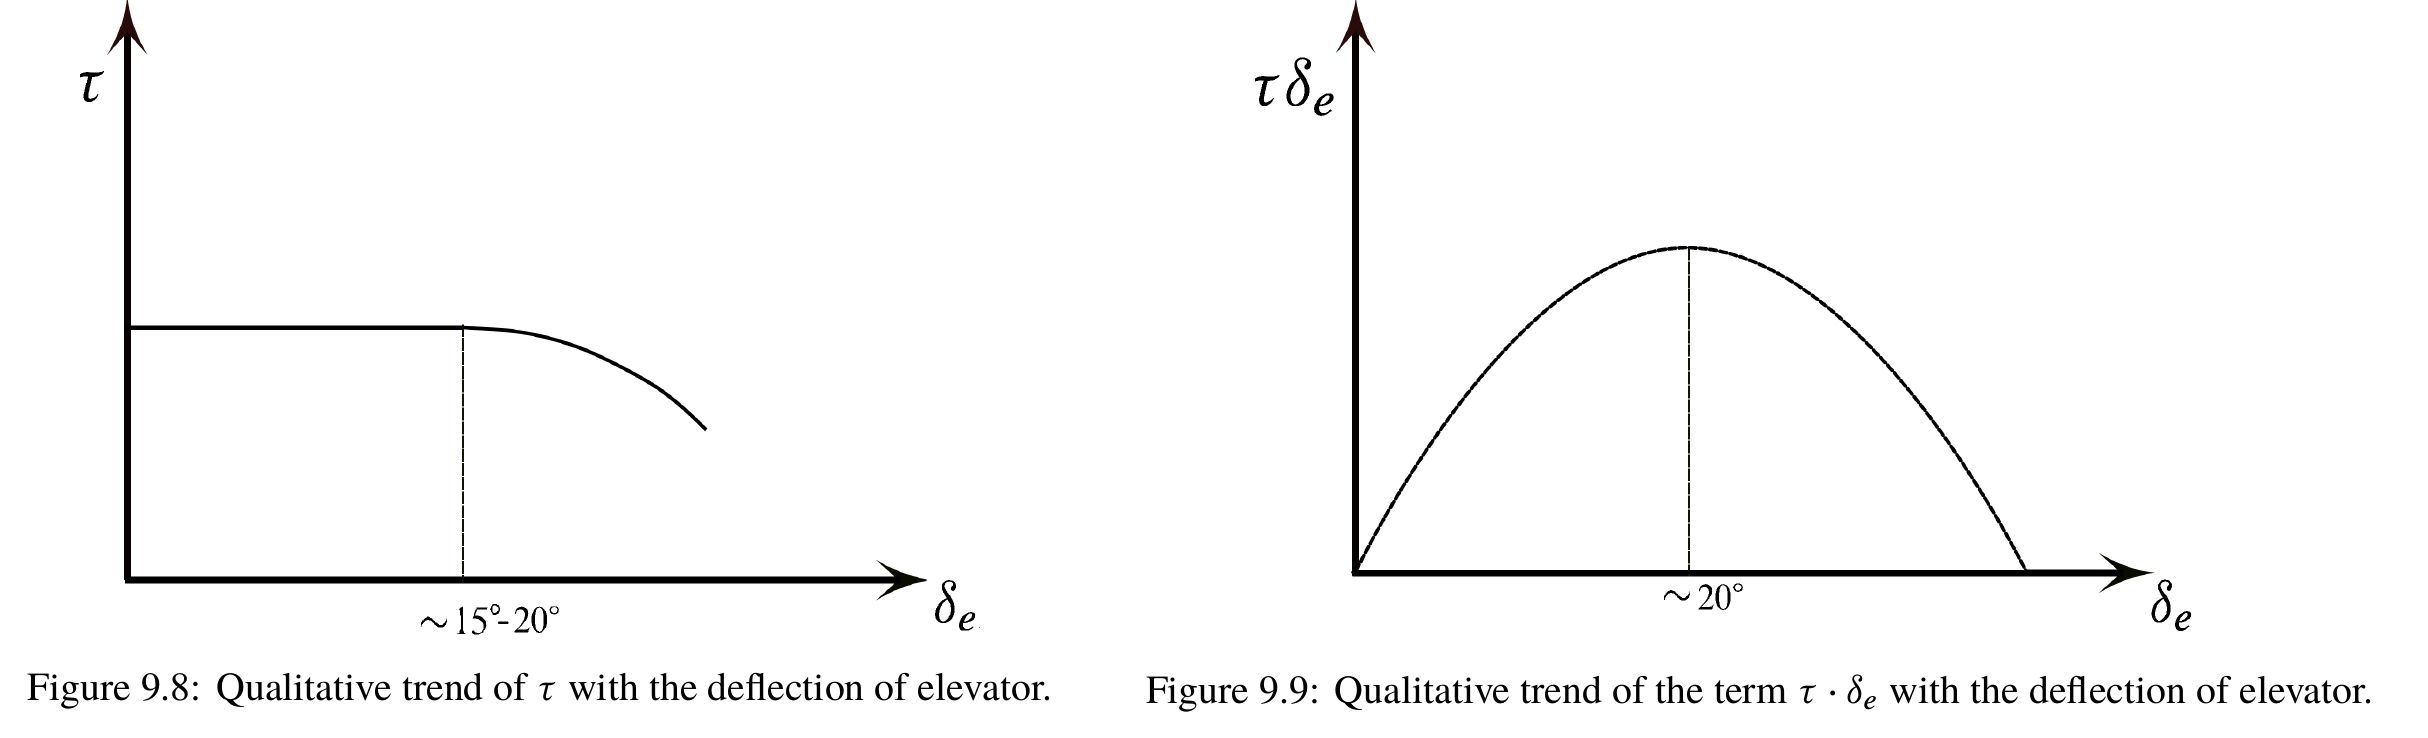
\includegraphics[height=4.9cm]{Immagini/tau.png}} 
%\label{tau3}
%\end{figure} 		


		
The evaluation of tau is made by reading of external database, considering the following graphs.
	
\begin{equation}
\tau = \alpha_{\delta} \eta_{\delta} = \frac{\alpha_{{\delta}_{c_L}}}{\alpha_{{\delta}_{c_l}}}\alpha_{{\delta}_{c_l}} \eta_{\delta}
\end{equation}

% scrivi che preso da qui i parametri

%\begin{figure}[H]
%\centering
%{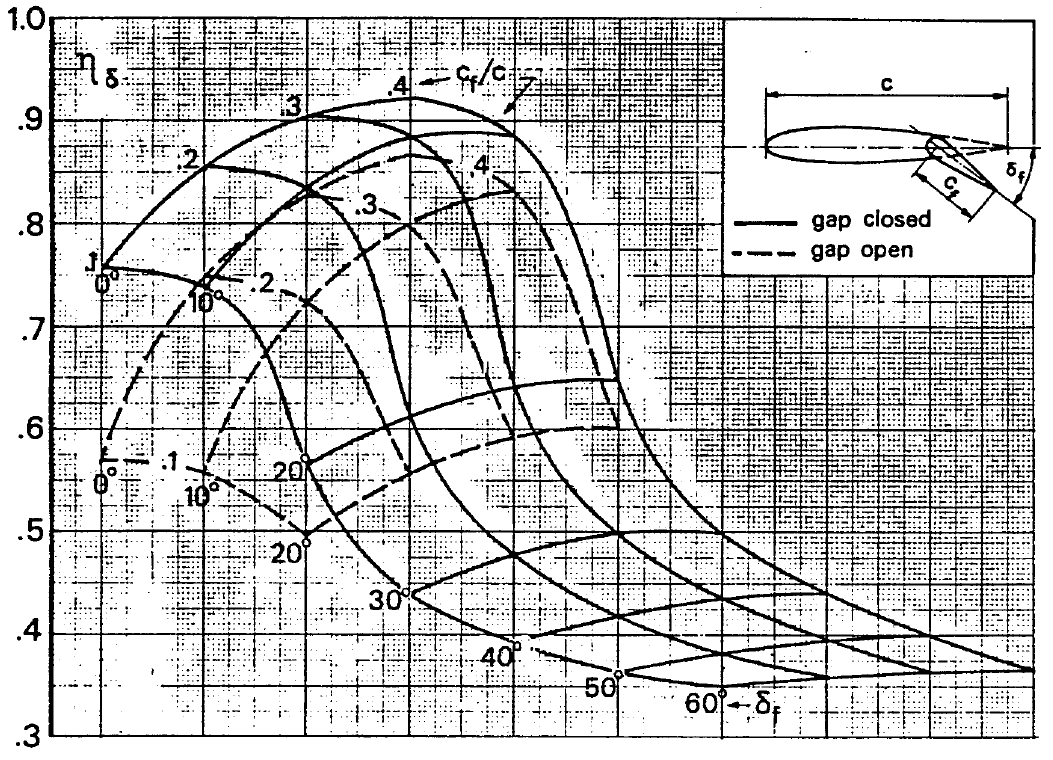
\includegraphics[height=6cm]{Immagini/Eta_Delta_Plain.png}} 
%\caption{2D efficiency correction for elevator.}
%\label{efficiency}
%\end{figure} 		
%
%
%\begin{figure}[H]
%\centering
%{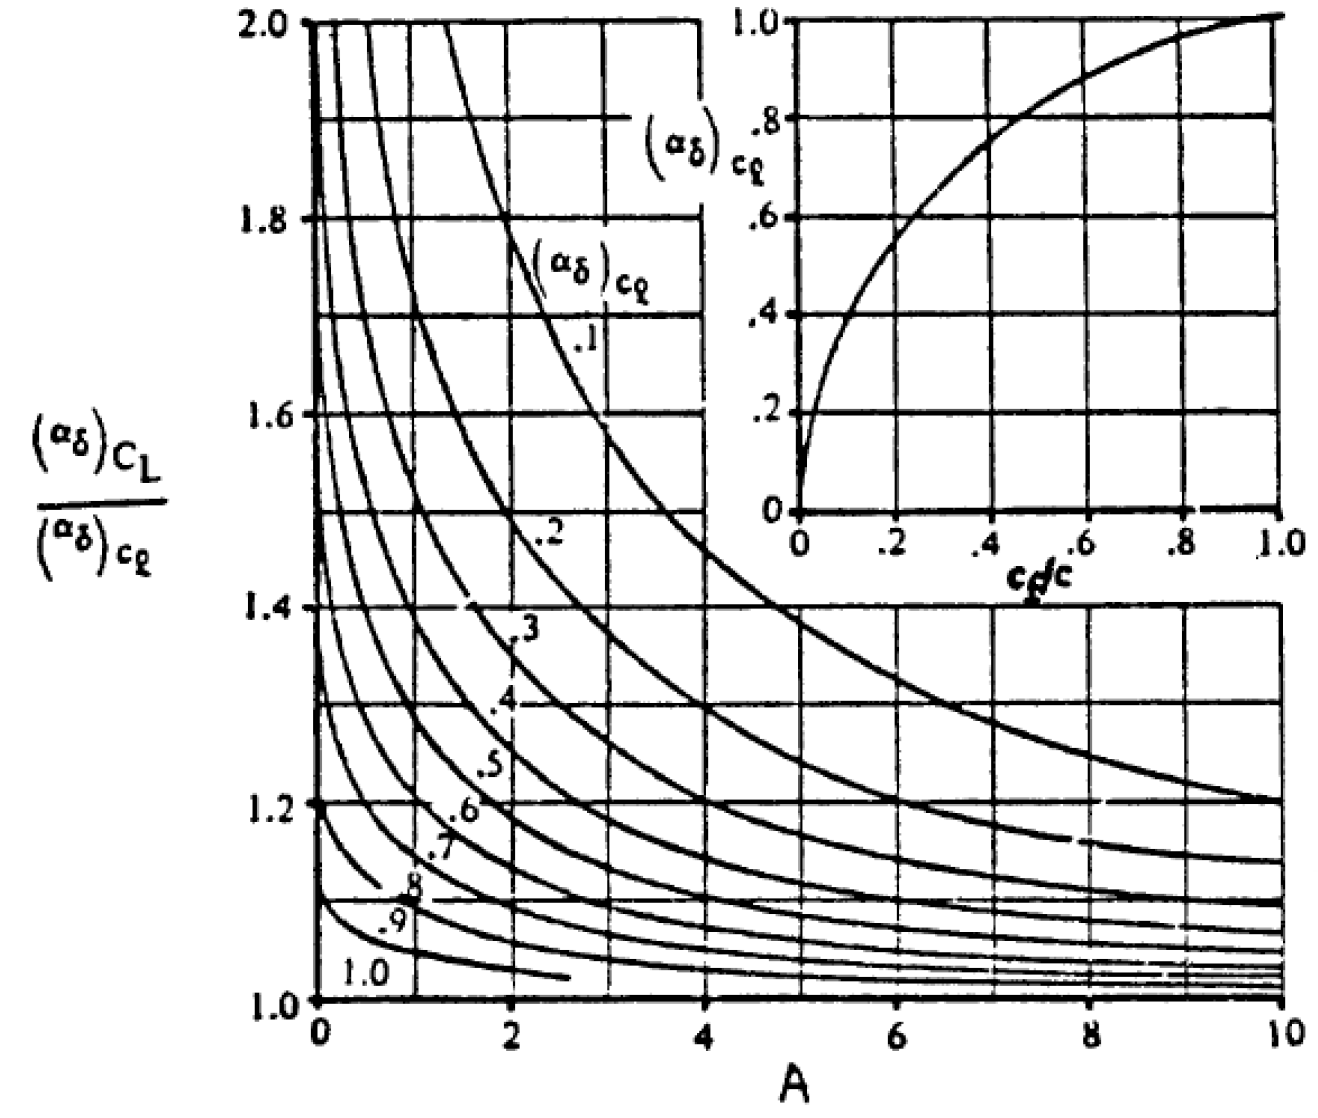
\includegraphics[height=6cm]{Immagini/alfadelta.png}} 
%\caption{$\frac{d \alpha_{0l}}{d \delta_e}$ 2D and 3D correction.}
%\label{efficiency}
%\end{figure} 		


\begin{figure}[H]
\centering
\begin{minipage}{.5\textwidth}
\centering
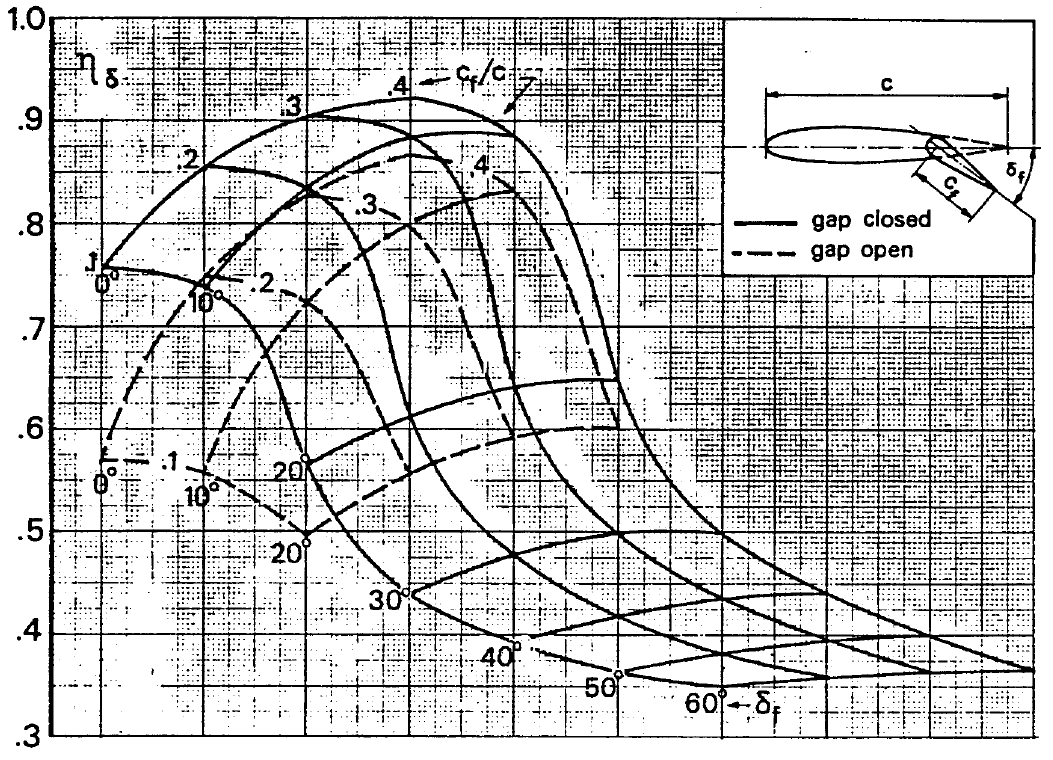
\includegraphics[height=5.4cm]{Immagini/Eta_Delta_Plain.png}
\captionof{figure}{2D efficiency correction for elevator.}
\label{efficiency}
\end{minipage}%
\begin{minipage}{.5\textwidth}
\centering
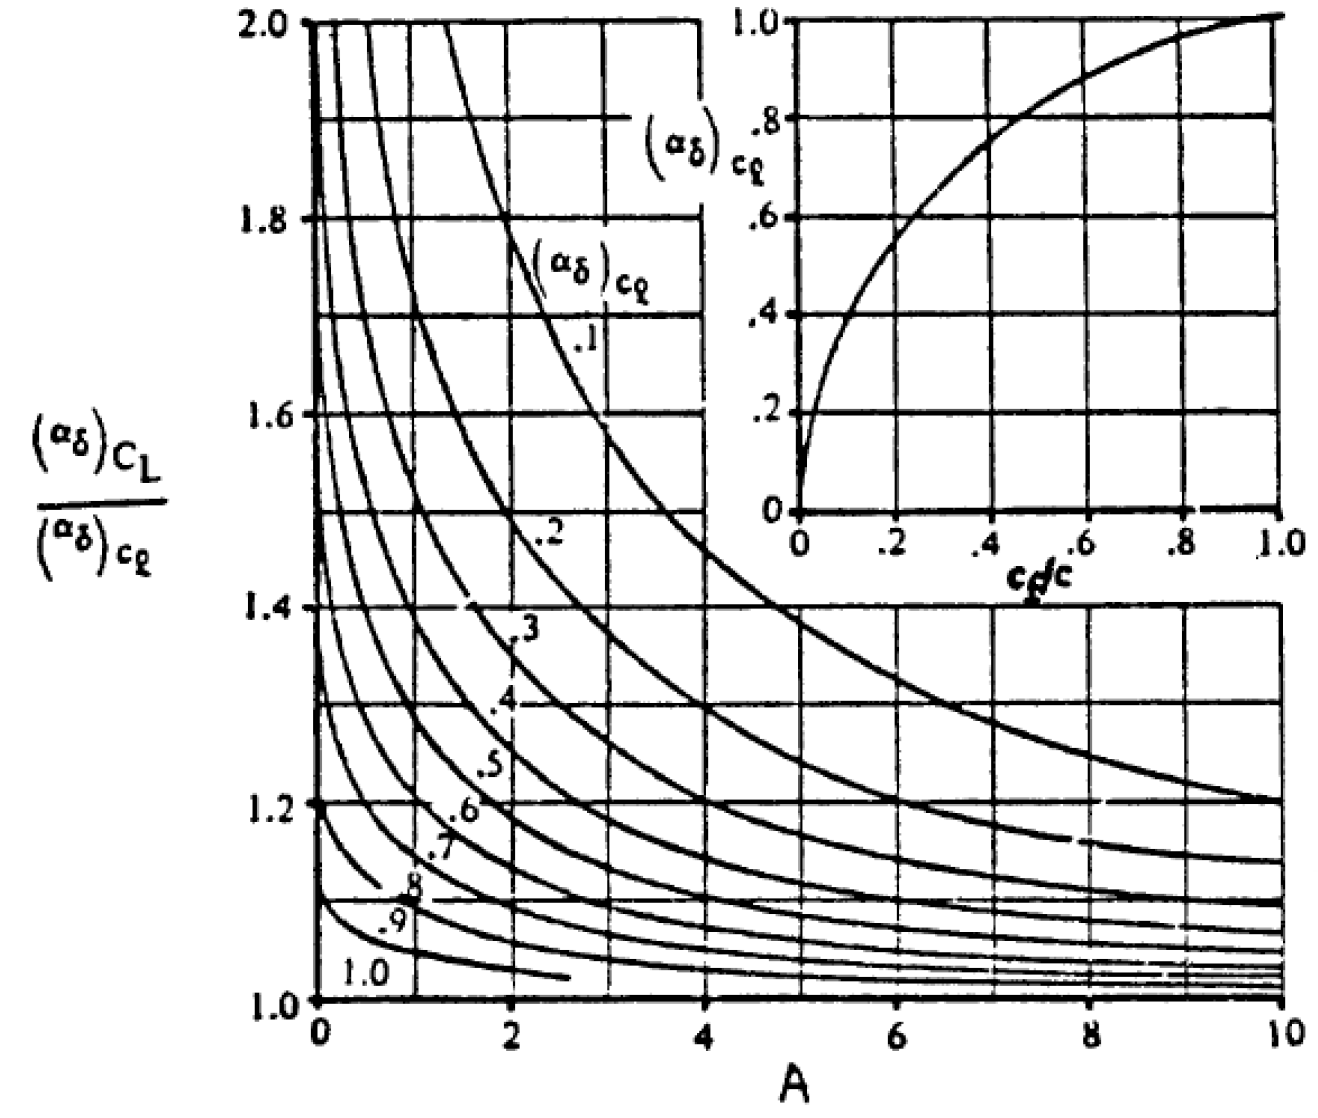
\includegraphics[height=5.4cm]{Immagini/alfadelta.png}
\captionof{figure}{$\frac{d \alpha_{0l}}{d \delta_e}$ 2D and 3D correction.}
\label{eff2}
\end{minipage}
\label{fig:effects}
\end{figure}

\noindent \\
The construction of the $C_L$ vs $\alpha$ curve is made as follows for each value of elevator deflection.
\begin{enumerate}
	\item It's necessary to know the value of $C_{L_{\alpha}}$ and $\alpha_{0L}$ clean
	\item The  $\alpha_{{0L}_{\delta_e}}$ is obtained starting from the $\tau$ value
	\begin{equation}
	\alpha_{{0L}_{\delta_e}} = \alpha_{{0L}_{clean}} - (\tau \delta_e)
	\end{equation}
	\item In order to evaluate the variation in $C_{L\alpha}$ due to elevator deflection, references to~\cite{torenbeek1982synthesis} have been made. In particular, Torenbeek provides the following equation which approximates the results of the exact theory fairly accurately and is in qualitative agreement with experimental data. 
	%
	\begin{equation}
	C_{l\alpha_{\left(\text{flap down}\right)}}=C_{l\alpha}\ \left[\dfrac{c'}{c}\ \left(1-\dfrac{c_f}{c'}\ \sin^2\delta_f\right)\right]
	\label{eqn:ClalphaFlap}
	\end{equation}
	%
	\noindent
	This equation is then corrected for the three-dimensional wing as follows.
	%
	\begin{equation}
	C_{L\alpha_{\left(\text{flap down}\right)}}=C_{L\alpha}\ \left\{1+\dfrac{\upDelta C_{L0}}{\upDelta C_{l0}}\ \left[\left(\dfrac{c'}{c}\ \left(1-\dfrac{c_f}{c'}\sin^2\delta_f\right)-1\right)\right]\right\}
	\label{eqn:ClalphaFlap}
	\end{equation}
	\item The new value of $C_{L_0}$ is obtained from the following equation
	\begin{equation}
	C_{L_0} = - C_{L\alpha_{\delta_e}} \alpha_{{0L}_{\delta_e}}
	\end{equation}
	\item The $\upDelta$ is obtained from High Lift modulus. An empirical method for predicting airfoil maximum lift increments for plain and slotted flaps is presented in DATCOM and will be followed from~\cite{sforza2014commercial}.
	%
	The maximum lift increment provided to an airfoil by the deflection of a trailing edge flap is given by the (\ref{eqn:DeltaClmaxFlap}).
	%
	\begin{equation}
	\upDelta C_{l\text{max}}=k_1\ k_2\ k_3\ \left(\upDelta C_{l\text{max}}\right)_{\text{base}}
	\label{eqn:DeltaClmaxFlap}
	\end{equation}
	%
	\noindent
	Here $\left(\upDelta C_{l\text{max}}\right)_{\text{base}}$ is the section maximum lift increment for 25 percent-chord flaps at the reference flap-deflection angle. The quantity $k_1$ is a factor accounting for flap-chord-to-airfoil-chord ratios, $\frac{c_{f}}{c}$, other than 0.25. The quantity $k_2$ is a factor accounting for flap deflections other than the reference value. Finally, $k_3$ is a factor accounting for flap motion as a function of flap deflection.
	\item The value of $\alpha_{stall}$ is obtained considering the same $\upDelta$ of clean lifting surface between the linear $\alpha_{max}$  and non linear $\alpha_{stall}$ .
\end{enumerate}


%\begin{figure}[H]
%\centering
%{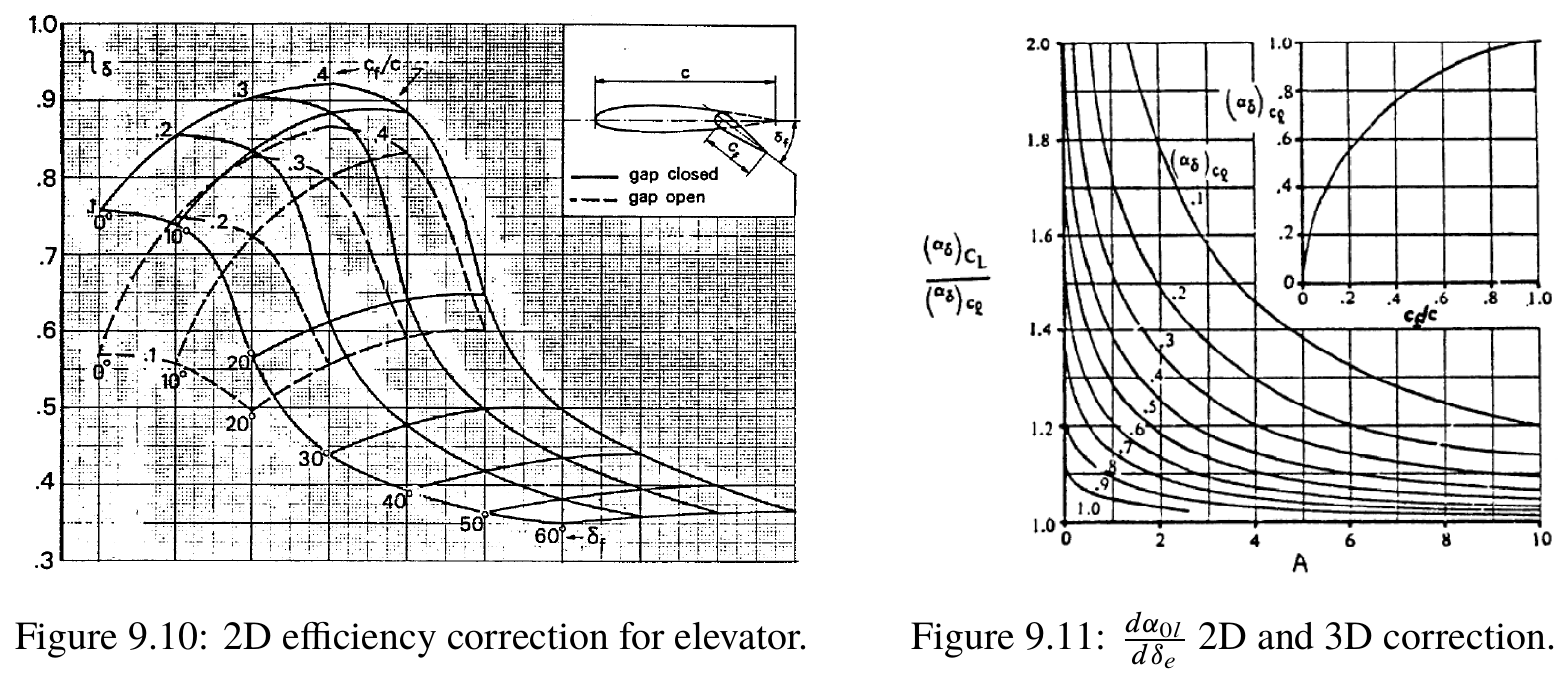
\includegraphics[height=6.79cm]{Immagini/alfadeltanew.png}} 
%\label{efficiency}
%\end{figure} 		


		
% java class archiecture(?)
%tabella elenco metodi con classe e che fanno

% descrizione

% spiegazione  (da fare) del calcolo del cl at alfa simile a quello dell ala
% spiegazione (da fare )  metodo calcolo tau in stability calculator
% spiegazione (gia fatta) del metodo calculateclwithdeflection in ls aerodynamic

% grafici con risultati

\subsection{Complete Aircraft}

In order to evaluate the lift coefficient of the entire airplane it's possible to consider it as consisting of the following parts\cite{ roskam2002airplane}:

\begin{itemize}
\item Wing and Fuselage
\item Horizontal Tail
\item Canard
\end{itemize}

It's important to consider the effective angles of attack in which the surfaces work. This is made considering the angles of incidence of the lifting surfaces and the downwash angle aft of the wing. An horizontal tail and a canard may be equipped with a trailing edge control surface. So in order to evaluate these contributes it's important to know the angle of deflection $\delta$ of these control surfaces.\\
The calculation of the individual contributions is reported in the relevant sections. In this section will be shown the method to evaluate the aircraft lift coefficient, known the single contributes.\\
For an aircraft with no canard, the formula is the following:

\begin{equation}
C_L = C_{L_{wb}} + \frac{S_t}{S_w} \eta_t C_{L_{t}}
\end{equation}

\noindent \\ 
Where $\eta_t$ is the ratio of dynamic pressure, called {\itshape tail efficiency factor}. In fact the dynamic pressure seen by horizontal tail differs from the free stream dynamic pressure due to two main reasons: the combination wing-fuselage and the presence of the propeller. The dynamic pressure of the tail depends on the location of the tail. If the tail is in the wake of the wing-body, the local dynamic pressure will be less than the free-stream because the flow gradually loses its kinetic energy. While if the tail is in the slipstream of propeller, the local dynamic pressure may increase due to the power absorbed by the propeller.



\section{Aerodynamic Drag}
The drag of an aircraft depends on its shape and speed, which are design-dependent, as well as on the properties of air, which are nature-dependent. Drag is a complex phenomenon arising from several sources, such as the viscous effects that result in skin friction and pressure differences as well as the induced flow field of the lifting surfaces and compressibility effects. \\
The aircraft drag estimate starts with the isolated aircraft components. Each component of the aircraft generates drag largely dictated by its shape. Total aircraft drag is obtained by summing the drag of all components plus their interference effects when the components are combined. It is important to note that the drag of two isolated bodies increases when they are brought together due to the interference of their flow fields.\cite{kundu}

\begin{figure}[H]
\centering
{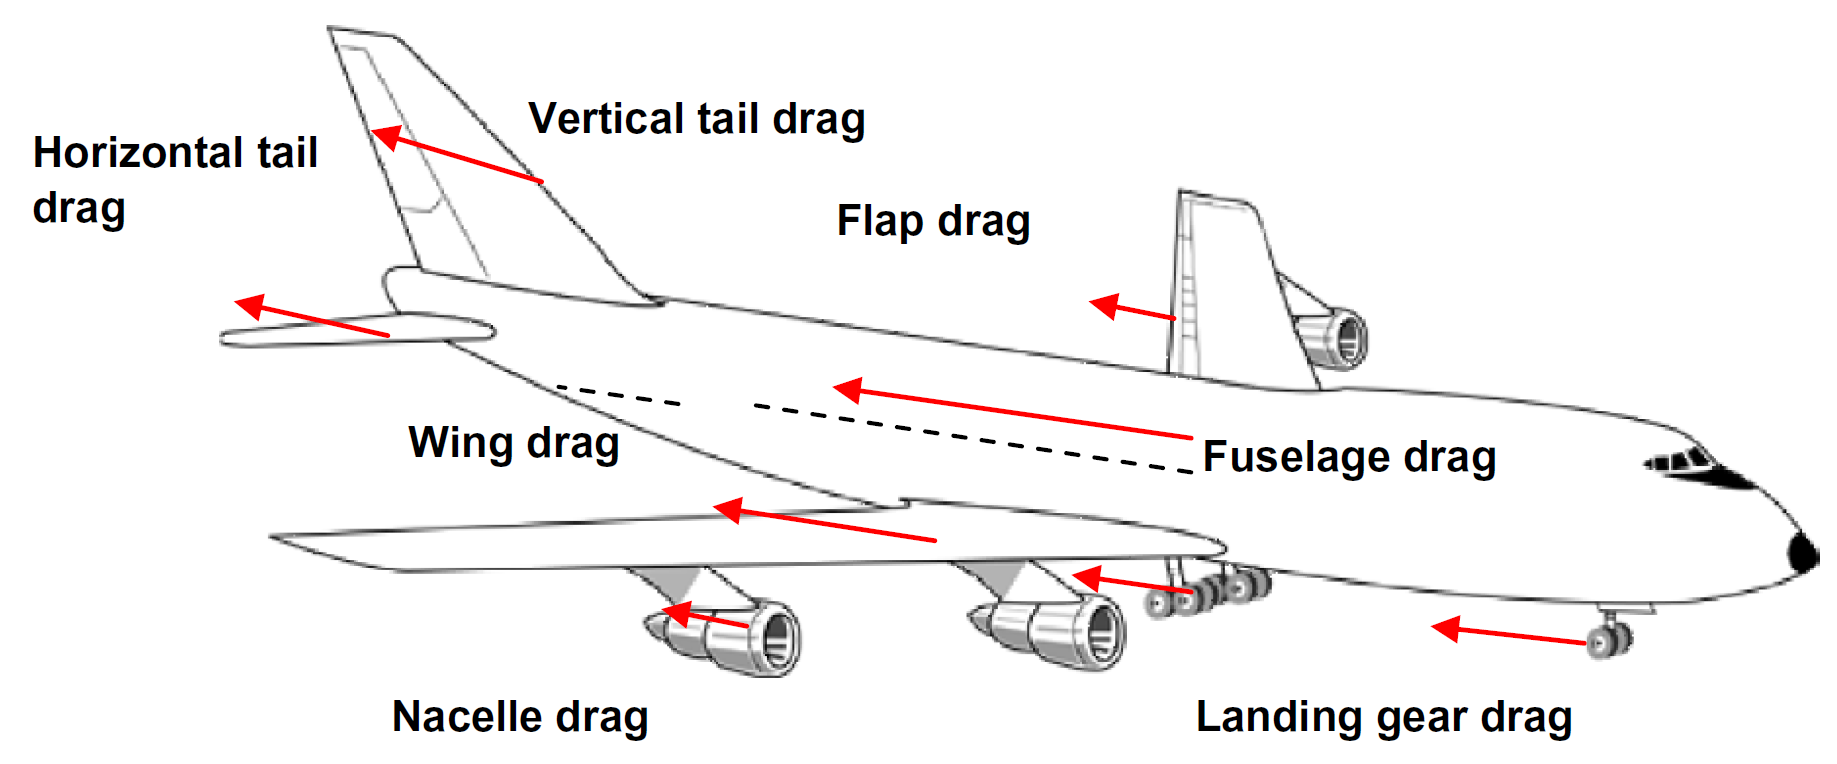
\includegraphics[height=5.6cm]{Immagini/dragcomponent.png}} 
\label{drag}
\caption{Drag components making up the total commercial airplane drag.\cite{sforza2014commercial}}
\end{figure} 		

In this thesis work, in order to evaluate the pitching moment coefficient of an aircraft has been considered the drag forces due to wing and horizontal tail.

\subsection{Drag of a lifting surface}

As widely expressed in the CHAPT  \ref{ch:wingdrag}, the drag coefficient of a lifting surface is calculated starting from the drag coefficient of the airfoils, expressed by the following equation:

\begin{equation}
CD = CD_{min} + (CL - CL_{CD_{min}})^2 \cdot k
\end{equation}

For each station, known the semi-spanwise lift distribution, it is possible to calculate the local lift coefficient of the intermediate airfoil and, consequently, the drag parasite coefficient. The induced drag is calculated starting from induced angle of attack. After the drag coefficient of the entire lifting surface is calculated with an integral.

\subsection{Additional drag due to elevator}

For the horizontal tail it is necessary to consider the additional drag due to the elevator deflection. It is possible to consider the elevator as a {\itshape plain flap} and use the concerning methods. \\
A plain flap is a high lift devices where a portion of the rear of a wing is simply hinged. The effectiveness of the flap derives from the fact that on rotation it changes the camber of the section and so permits of a change of circulation and therefore, of lift at a given incidence. \\
The increment in profile drag coefficient due to a flap at a given incidence is rather more influenced by test conditions than is the lift coefficient
increment. Nevertheless, the influence of test conditions and wing incidence is still sufficiently small over a wide range of incidence for us to accept the increment at a standard incidence as a reliable measure of the profile drag characteristics of a flap. \cite{Young:Flaps} The increment of drag is a $\upDelta CD_0$
Young and Hufton assumed that  $\upDelta C_D0$ can be calculated as follow for a full-span flap:
%
\begin{equation}
\upDelta C_{D0}=\delta_1\left(c_f/c\right)\cdot\delta_2\left(\delta_f\right)
\label{eqn:DeltaCD0FullSpan}
\end{equation}
%
where $\delta_1$ and $\delta_2$ are functions that were determined from experimental data. Their related curves are shown in figure~\ref{fig:Delta1Plain} and~\ref{fig:Delta2Plain} for plain flap.
%
\begin{figure}[H]
\centering
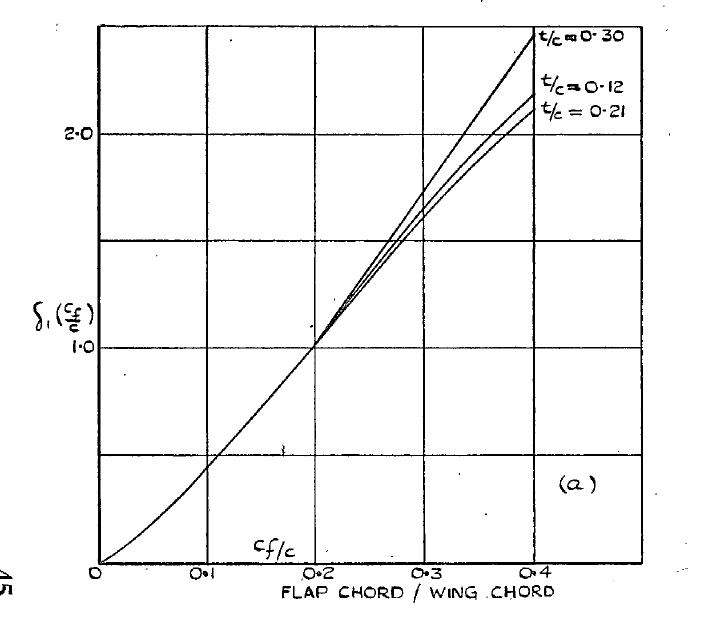
\includegraphics[height=7.9cm]{Immagini/Delta1_Plain}
\caption{The functions $\delta_1\left(c_f/c\right)$ for split and plain flaps}
\label{fig:Delta1Plain}
\end{figure}
%
\begin{figure}[H]
\centering
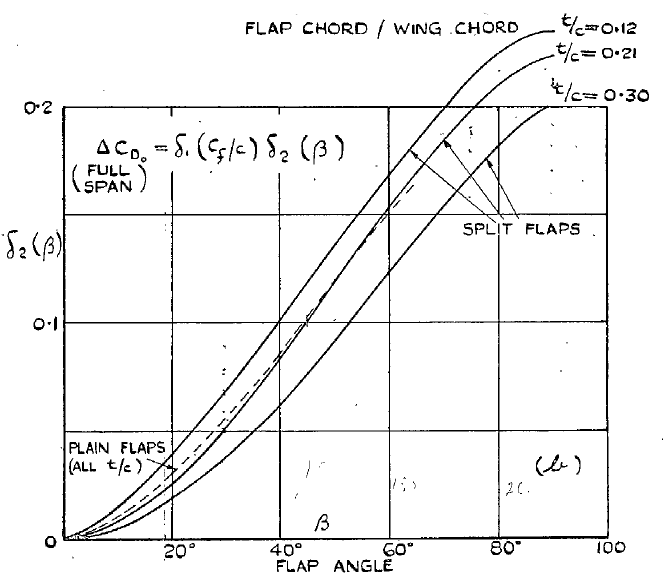
\includegraphics[height=7.9cm]{Immagini/Delta2_Plain}
\caption{The functions $\delta_2\left(\delta_f\right)$ for plain flaps}
\label{fig:Delta2Plain}
\end{figure}
%


\section{Pitching Moments}
The purpose of this section is to explain the followed procedure used to evaluate the pitching coefficient moments of the aircraft components.\\
Due to the interaction between the body and the flow a pressure distribution is generated whose result is the aerodynamic force acting at the center of pressure. In consequence of what there is a pitching moment that is a moment acting on the pitch axis of a moving body. \\
As the angle of attack changes on a cambered airfoil, there is a movement of the center of pressure forward and aft.  One of the remarkable properties of a cambered airfoil is that, even though the center of pressure moves forward and aft, there is a point, called Aerodynamic Center, with respect to which the moment coefficient is constant. The aerodynamic center is the most convenient place to locate the lift, drag, and moment of an aircraft wing or airfoil section.\\
So, for each component of the aircraft, it will be calculated the pitching moment coefficient respect to its aerodynamic center.


%sforza224

% ridurre tutto allla corda media- nicolai
\subsection{Lifting surface}

In order to evaluate the pitching moment coefficient of a lifting surface, at a given angle of attack, the implemented process is the following.\\
First it is calculated the pitching moment coefficient respect to the point at a quarter of the mean aerodynamic chord. Starting from these values, to vary the angle of attack, it's possible to evaluate the position of aerodynamic center.

\begin{enumerate}

\item Fifty points are defined along the semi-span.
\item An intermediate airfoil is calculated for each point.
\item The lift coefficient is calculated with the local Cl vs  $\alpha$ curve for each airfoil at a given station. In this way it’s possible to consider both the linear trait and the non linear one.
\item The position of the center of pressure is calculated for each airfoil using the following equation

\begin {equation}
\frac{x_{CP}}{c} = \frac{x_{AC}}{c} - \frac{C_{M_{ac}}}{C_l}
\end{equation}

\item The arm between the local center of pressure and the point at a quarter of lifting surface’s MAC is calculated for each airfoil. The equations that define the MAC are the following:

\begin{equation}
MAC=\frac{2}{S} \int_{0}^{\frac{b}{2}} c^2\, dy
\end{equation}

\begin{equation}
x_{MAC}=\frac{2}{S} \int_{0}^{\frac{b}{2}}x_{le}(y) c(y)\, dy
\end{equation}

\begin{equation}
y_{MAC}=\frac{2}{S} \int_{0}^{\frac{b}{2}}y_{le}(y) c(y)\, dy
\end{equation}

\item Finally it’s possible to evaluate the pitching moment about the point at a quarter of MAC with the product between the lift force and the arm.
\end{enumerate}


Repeating the process to vary the angle of attack it's possible to estimate the slope of the pitching moment curve.  In fact, the aerodynamic center, is that point on an aircraft, wing, or airfoil section about which the pitching moment is independent of angle of attack.
If the slope is positive, the aerodynamic center is behind the quarter of the MAC, conversely if the slope is negative, the aerodynamic center is the quarter of the MAC is behind the aerodynamic center.

\begin{figure}[H]
\centering
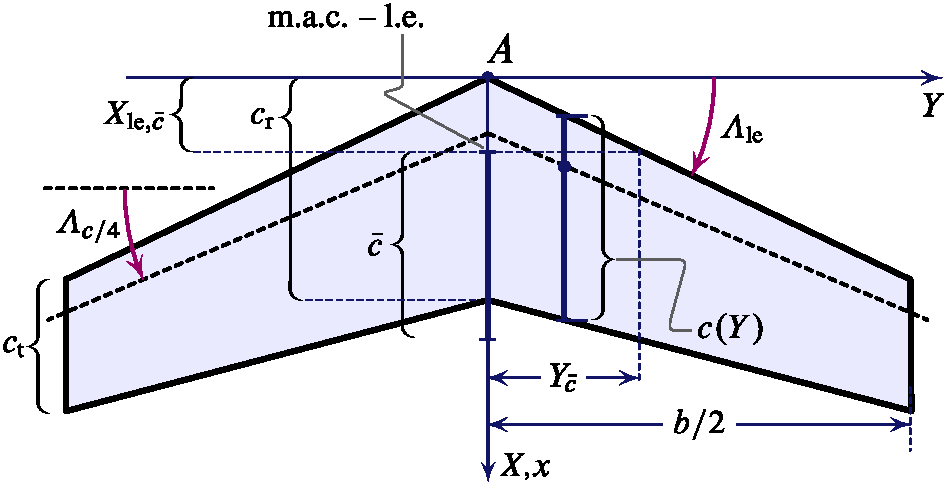
\includegraphics[height=7cm]{Immagini/wing_topview_1_new}
\caption{Wing topview definitions.}
\label{wing}
\end{figure}


\subsection{Additional moment due to elevator}
The horizontal tail is usually a symmetric section so that and $M_{ac_ht} = 0$ for $\delta_e = 0$. If there is a deflection of elevator it's necessary to consider a additional term. According to ~\cite{torenbeek1982synthesis}, the generalized expression, for airfoils, in (\ref{eqn:DeltaCm}) represents a useful starting point when experimental data are not available.
%
\begin{equation}
\upDelta C_{m_{\frac{c}{4}}}=-\mu_1\ \upDelta C_{l\text{max}}\ \left(\dfrac{c'}{c}\right)^2-\dfrac{C_l}{4}\ \dfrac{c'}{c}\left(\dfrac{c'}{c}-1\right)+\left(C_{m_{\frac{c}{4}}}\right)_{\delta_f=0}\ \left[\left(\dfrac{c'}{c}\right)^2-1\right]
\label{eqn:DeltaCm}
\end{equation}
%
where extended chord $c'$ allows for the effects of the backward movement of the flap while it is being extended.
%
In this equation, the first contribution is due to the increased section camber and the factor $\mu_1$ is defined as follows according to Glauert's linear theory for small flap deflections.
%
\begin{equation}
\mu_1=\dfrac{1}{2}\left(1-\dfrac{c_f}{c}\right)\dfrac{\sin\theta_f}{\pi-\left(\theta_f-\sin\theta_f\right)}
\label{eqn:Mu1}
\end{equation}
%
This theoretical value of $\mu_1$ generally underpredicts the pitching moment coefficient; in fact it has been found that, for slotted flaps with, or without, Fowler movement, most data are on a single line, provided the second term of the equation (\ref{eqn:Mu1}), representing the theoretical rearward shift of the airfoil aerodynamic center, is halved. Furthermore, in the case of split and plain flaps, the flap angle is observed to exert a pronounced influence on $\mu_1$ as shown in figure~\ref{fig:Mu1}.

The last term of the (\ref{eqn:Mu1}) is generally of a low order and can be ignored. This, together with the halving of the second term of the previous equation, leads to the following practical expression of $\upDelta C_{m_{\frac{c}{4}}}$.
%
\begin{equation}
\upDelta C_{m_{\frac{c}{4}}}=-\mu_1\ \upDelta C_{l\text{max}}\ \left(\dfrac{c'}{c}\right)-\dfrac{C_l}{8}\ \dfrac{c'}{c}\left(\dfrac{c'}{c}-1\right)
\label{eqn:DeltaCmPractical}
\end{equation}

\bigskip
\noindent
The obtained two-dimensional equation can, then, be converted into a three-dimensional one, which computes the pitching moment change on the entire wing, as follows.
%
\begin{equation}
\upDelta C_{M_{\frac{c}{4}}}=\mu_2\ \upDelta C_{m_{\frac{c}{4}}}+0.7\ \dfrac{\AR}{1+\frac{2}{\AR}}\ \mu_3\ \upDelta C_{l_{\text{max}}}\ \tan\Lambda_{\frac{c}{4}}
\label{eqn:DeltaCM}
\end{equation}
%
where $\upDelta C_{m_{\frac{c}{4}}}$ is the one from (\ref{eqn:DeltaCmPractical}), provide that $C_l=C_L+\upDelta C_{l\text{max}}\ \left(1-\frac{S_{w,f}}{S}\right)$, and the correction factors $\mu_2$ and $\mu_3$ are the one shown in figures~\ref{fig:Mu2} and~\ref{fig:Mu3}. Making the appropriate substitutions, the following operational formula is, finally, obtained.
%

\begin{figure}[H]
\centering
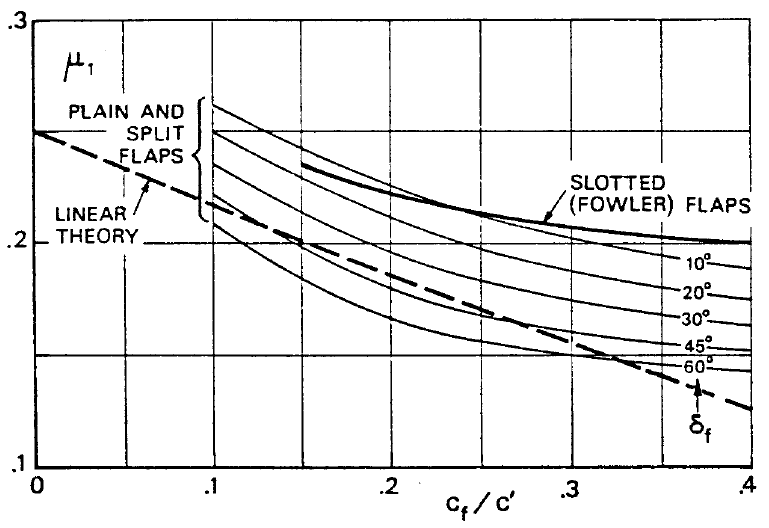
\includegraphics[width=0.75\linewidth]{Immagini/Mu1_Pitching_Moment}
\caption{The pitching moment function $\mu_1$}
\label{fig:Mu1}
\end{figure}
%
\begin{figure}[H]
\centering
\begin{minipage}{.5\textwidth}
\centering
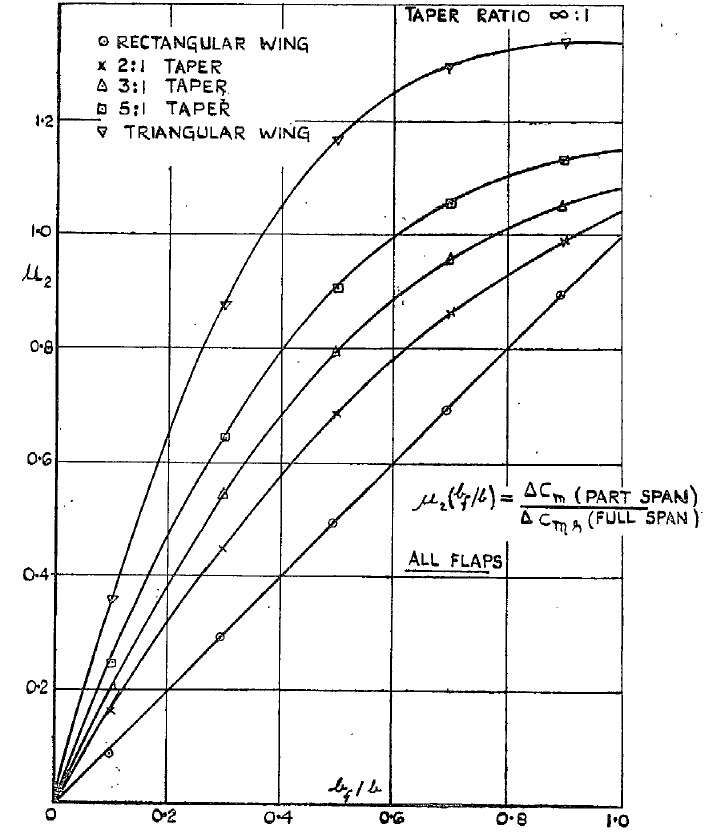
\includegraphics[width=1.1\linewidth]{Immagini/Mu2_Pitching_Moment}
\captionof{figure}{The pitching moment function $\mu_2$}
\label{fig:Mu2}
\end{minipage}%
\begin{minipage}{.5\textwidth}
\centering
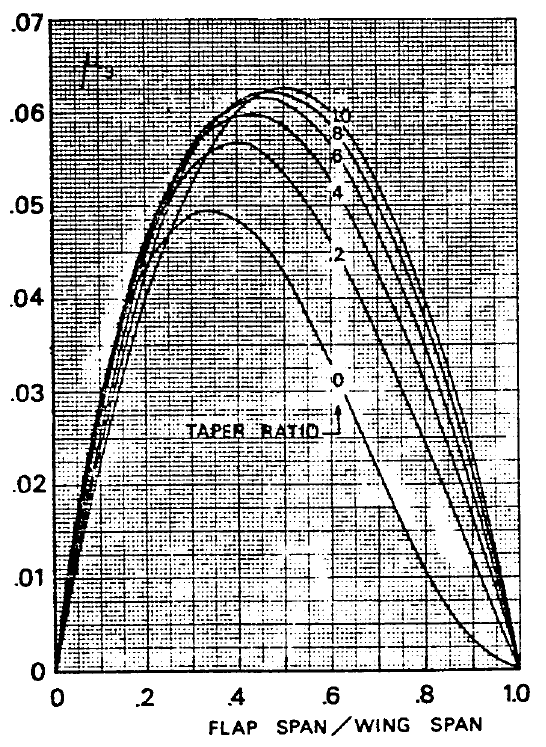
\includegraphics[width=0.94\linewidth]{Immagini/Mu3_Pitching_Moment}
\captionof{figure}{The pitching moment function $\mu_3$}
\label{fig:Mu3}
\end{minipage}
\end{figure}
%
\begin{equation}
\begin{split}
\upDelta C_{M_{\frac{c}{4}}}&=\mu_2\ \left\{-\mu_1\ \upDelta C_{L\text{max}}\ \dfrac{c'}{c}-\left[C_L+\upDelta C_{l\text{max}}\left(1-\dfrac{S_{w,f}}{S}\right)\right]\dfrac{1}{8}\ \dfrac{c'}{c}\left(\dfrac{c'}{c}-1\right)\right\}\\
&\quad+0.7\ \dfrac{\AR}{1+\frac{\AR}{2}}\ \mu_3\ \upDelta C_{l\text{max}}\ \tan\Lambda_{\frac{c}{4}}
\label{eqn:DeltaCMPractical}
\end{split}
\end{equation}


\subsection{Fuselage}
The moment coefficient of the fuselage is a pure couple, so it is not necessary to specify the pole.


\begin{figure}[H]
\centering
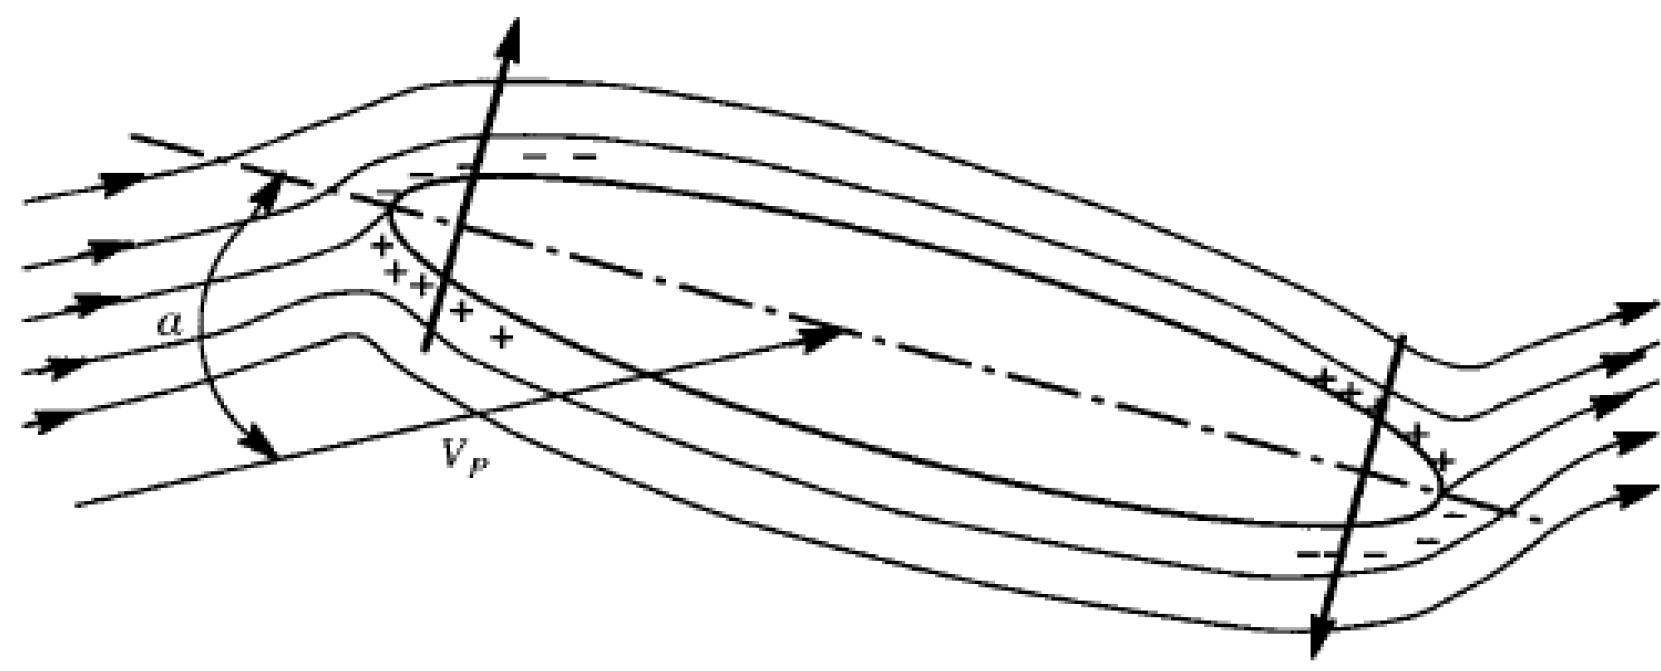
\includegraphics[height=4cm]{Immagini/fuse}
\caption{Fuselage in potential flow at angle of attack.}
\label{fus}
\end{figure}


Assuming the linearity, is possible to represented the pitching moment coefficient by the following equation in function of the angle of attack.

\begin{equation}
C_{M_f}=C_{M_{0_f}}+C_{{M\alpha}_f} \alpha_{body}
\label{eq:fus}
\end{equation}

In JPAD it's possible to evaluate these two contributes using different methods.

\subsubsection{Multhopp method}

Each term in the equation \ref{eq:fus} can be calculated by the Multhopp method. % Multhopp has developed a method of calculating the local lift and pitching moment on wings of any plan-form in subsonic steady flow.  
The fuselage is divided into strips, each of which gives a contribution to the pitching moment according to its distance from the wing.

The two coefficients $C_{M_{0_f}}$  and $C_{{M\alpha}_f}$ in eq. \ref{eq:fus} can be obtained from the following equations.

\begin{equation}
C_{M_{0}f}=\dfrac{K_2-K_1}{36.5\cdot S\cdot MAC}\cdot\int_0^{l_f} \! {W_f}^2\cdot\left(\alpha_{{0L}_w}+i_w+i_{{cl}_f}\right) \, \mathrm{d}x
\end{equation}

\begin{equation}
C_{{M\alpha}_f}=\dfrac{1}{36.5\cdot S\cdot MAC}\cdot \left\{ \int_0^{l_{f1}} \! {W_f}^2\cdot \left[ {\left( \dfrac{\partial \epsilon_u}{\partial \alpha} \right)}_1 +1\right] \, \mathrm{d}x_1 + \int_0^{l_{f2}} \! {W_f}^2\cdot \left[ {\left( \dfrac{\partial \epsilon_d}{\partial \alpha} \right)}_2 +1\right] \, \mathrm{d}x_2 \right\}
\end{equation}

Instead of the integrals it’s possible to substitute them with summations.

\begin{equation}
C_{M_{0}f}=\dfrac{K_2-K_1}{36.5\cdot S\cdot MAC}\cdot\sum_{j=1}^{n} \! {W_{f_j}}^2\cdot\left(\alpha_{{0L}_w}+i_w+i_{{cl}_f}\right)\cdot \Delta x;
\end{equation}

\begin{equation}
C_{{M\alpha}_f}=\dfrac{1}{36.5\cdot S\cdot MAC}\cdot \left\{ \sum_{j=1}^{n_1} \! {W_{f_j}}^2\cdot \left[ {\left( \dfrac{\partial \epsilon_u}{\partial \alpha} \right)}_1 +1\right] \cdot \Delta x_{1} + \sum_{j=1}^{n_2} \! {W_{f_j}}^2\cdot \left[ {\left( \dfrac{\partial \epsilon_d}{\partial \alpha} \right)}_2 +1\right] \cdot \Delta x_{2} \right\}
\end{equation}


\begin{figure}[H]
\centering
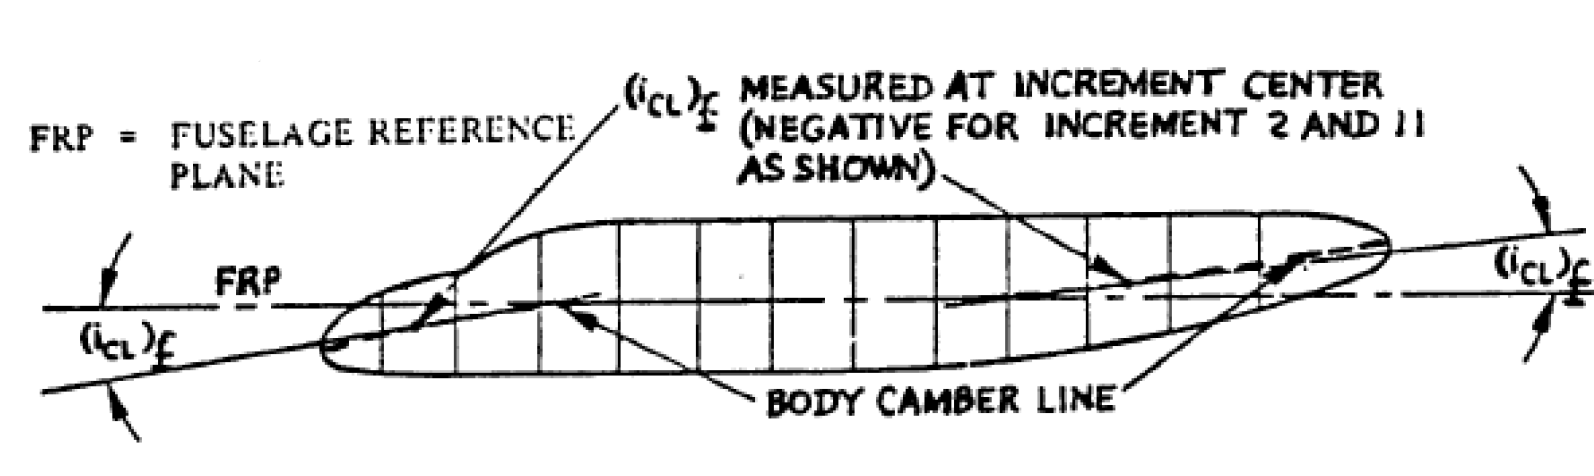
\includegraphics[height=3.1cm]{Immagini/stripszero}
\caption{Strips definition for the determination of $C_{M_{0_f}}$.}
\label{wing}
\end{figure}

\begin{figure}[H]
\centering
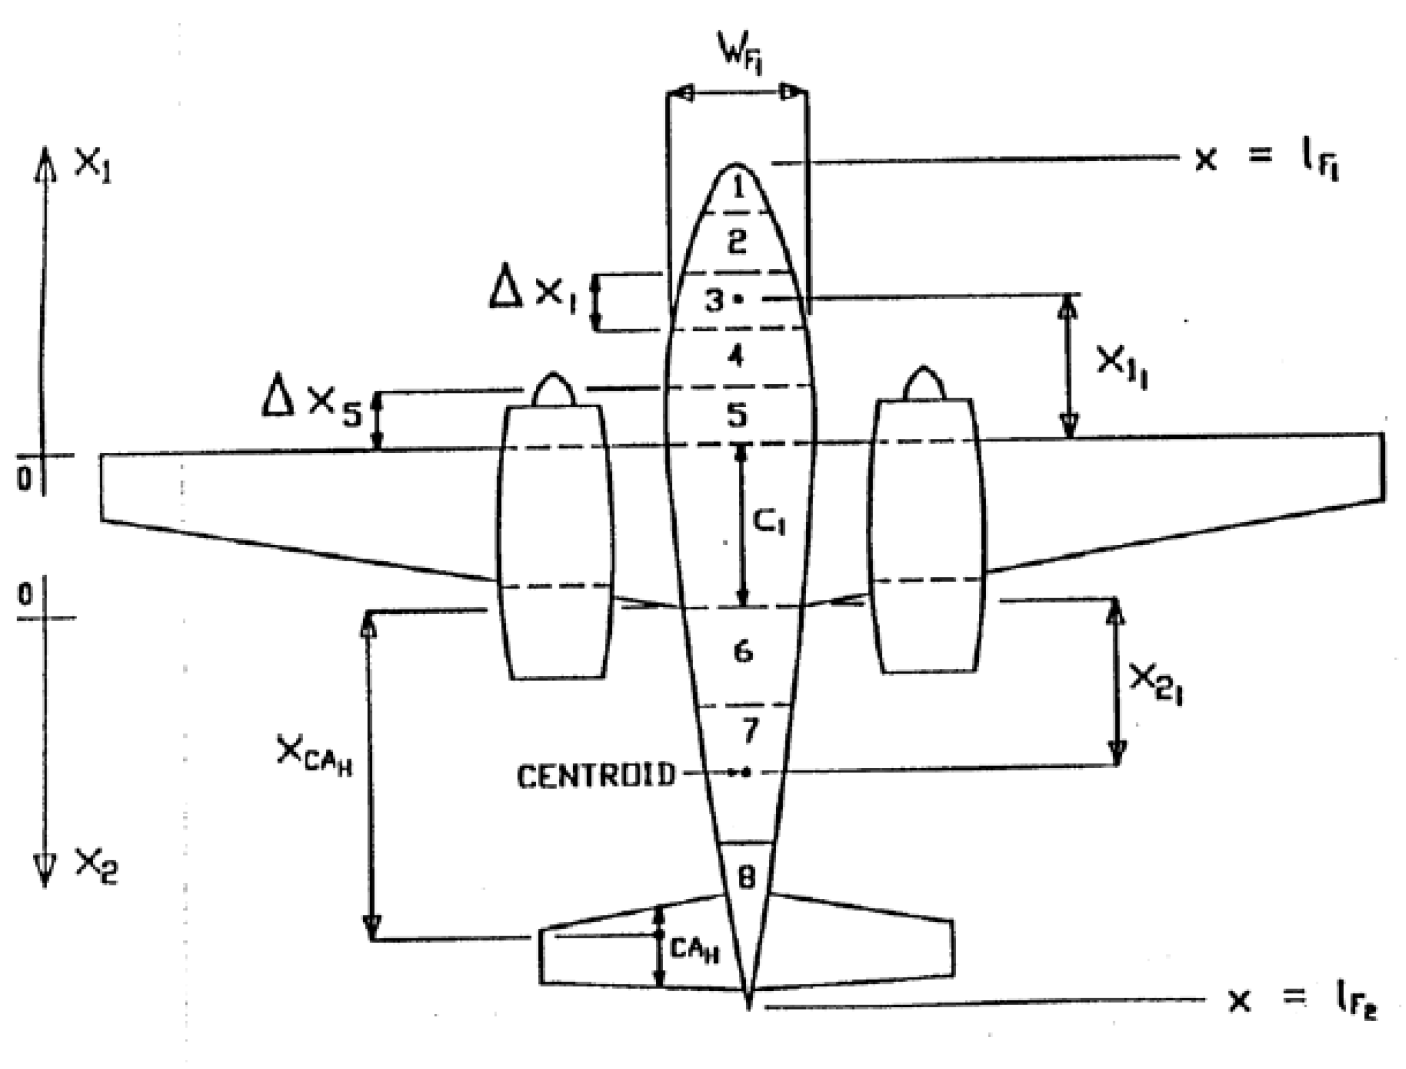
\includegraphics[height=6.3cm]{Immagini/stripsalfa}
\caption{Strips definition for the determination of $C_{{M\alpha}_f}$ .}
\label{wing}
\end{figure}


The parameter $K_2-K_1$ is a correction factor that is dependent on the value of the fineness ratio and is evaluated by the following figure.\cite{adas}


\begin{figure}[H]
\centering
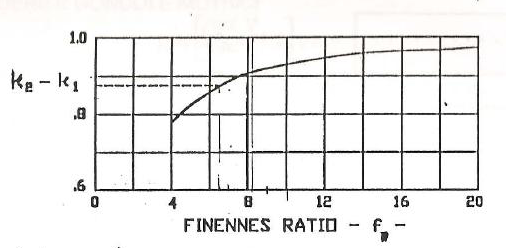
\includegraphics[height=4.3cm]{Immagini/kdue}
\caption{$K_2-K_1$ correction factor in function of fineness ratio.}
\label{kfactor}
\end{figure}

Dor stability it's necessary to evaluate the new aerodynamic center (wing-body) and the pitching moment coefficient respect to this point. In fact the fuselage introduces a shift of the aerodynamic center to the leading edge. 
It's possible to obtain the new aerodynamic center using the Eq. \ref{eq:aerc}

\begin{equation}
\upDelta X_{ac} = x_{ac_{wb}} - x_{ac_{w}} = -\frac{C_{M_{\alpha_f}}}{C_{L_{\alpha_f}}}
\label{eq:aerc}
\end{equation}

The wing-body pitching moment respect to the new aerodynamic center is :

\begin{equation}
C_{M_{ac_{wb}}} = C_{M_{ac_{w}}}  + C_{M_{0l_f}}
\end{equation}

\subsubsection{Fuselage Pitching moment prediction method}
This method has been developed in the Dept. of Industrial Engineering, University of Study of Naples Federico II, by numerical aerodynamic analyses performed with STAR-CCM+. \
From a reference fuselage layout the nose, cabin (constant fuselage diameter), and tailcone geometry have been parametrically changed. Then, the aerodynamic drag, the pitching moment at zero incidence, the longitudinal static stability derivative, and the yawing moment coefficients $C_D$, $C_{M_0}$, $C_{M_{\alpha}}$, and $C_{N_{\beta}}$ respectively, have been evaluated by numerical analysis. Aerodynamic effects of each component (nose, cabin, tailcone) have been directly obtained from the CFD aerodynamic solver, separating the forces and moments contributions of each fuselage part. \cite{fuselageunina}


\begin{figure}[H]
\centering
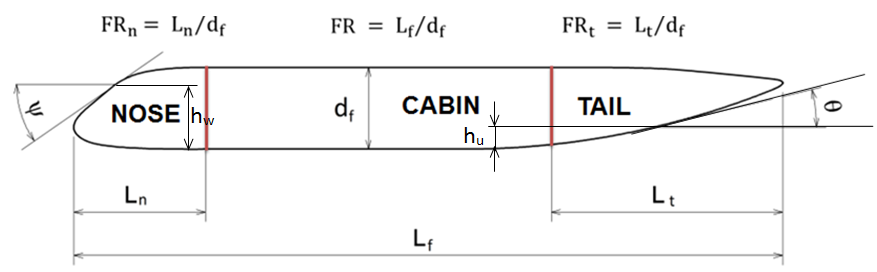
\includegraphics[height=4.6cm]{Immagini/fuselage}
\caption{Main fuselage geometrical parameters.}
\label{fusgeometry}
\end{figure}


The fuselage pitching moment coefficient can be estimated according to the equation \ref{eq:fus} where :

\begin{equation}
C_{M_{0_f}} = C_{M_{0_{FR}}} + \upDelta C_{M_{0_{NOSE}}} +  \upDelta C_{M_{0_{TAIL}}}
\end{equation}

\begin{equation}
C_{M_{{\alpha}_f}} = C_{M_{{\alpha}_{FR}}} + \upDelta C_{M_{{\alpha}_{NOSE}}} +  \upDelta C_{M_{{\alpha}_{TAIL}}}
\end{equation}

\noindent \\

where the subscript $FR$ refers to the pitching moment coefficient as function of fuselage fineness ratio. The subscript $NOSE$ the pitching moment nose correction factor. It depends on windshield angle $\Phi$ and on the nose fineness ratio $FR_n$. Finally the subscript $TAIL$ refers to the pitching moment tail correction factor. It depends on upsweep angle $\theta$ and on the tail fineness ratio $FR_t$.\\
The following figures show the variability of introduced parameters.

\begin{figure}[H]
\centering
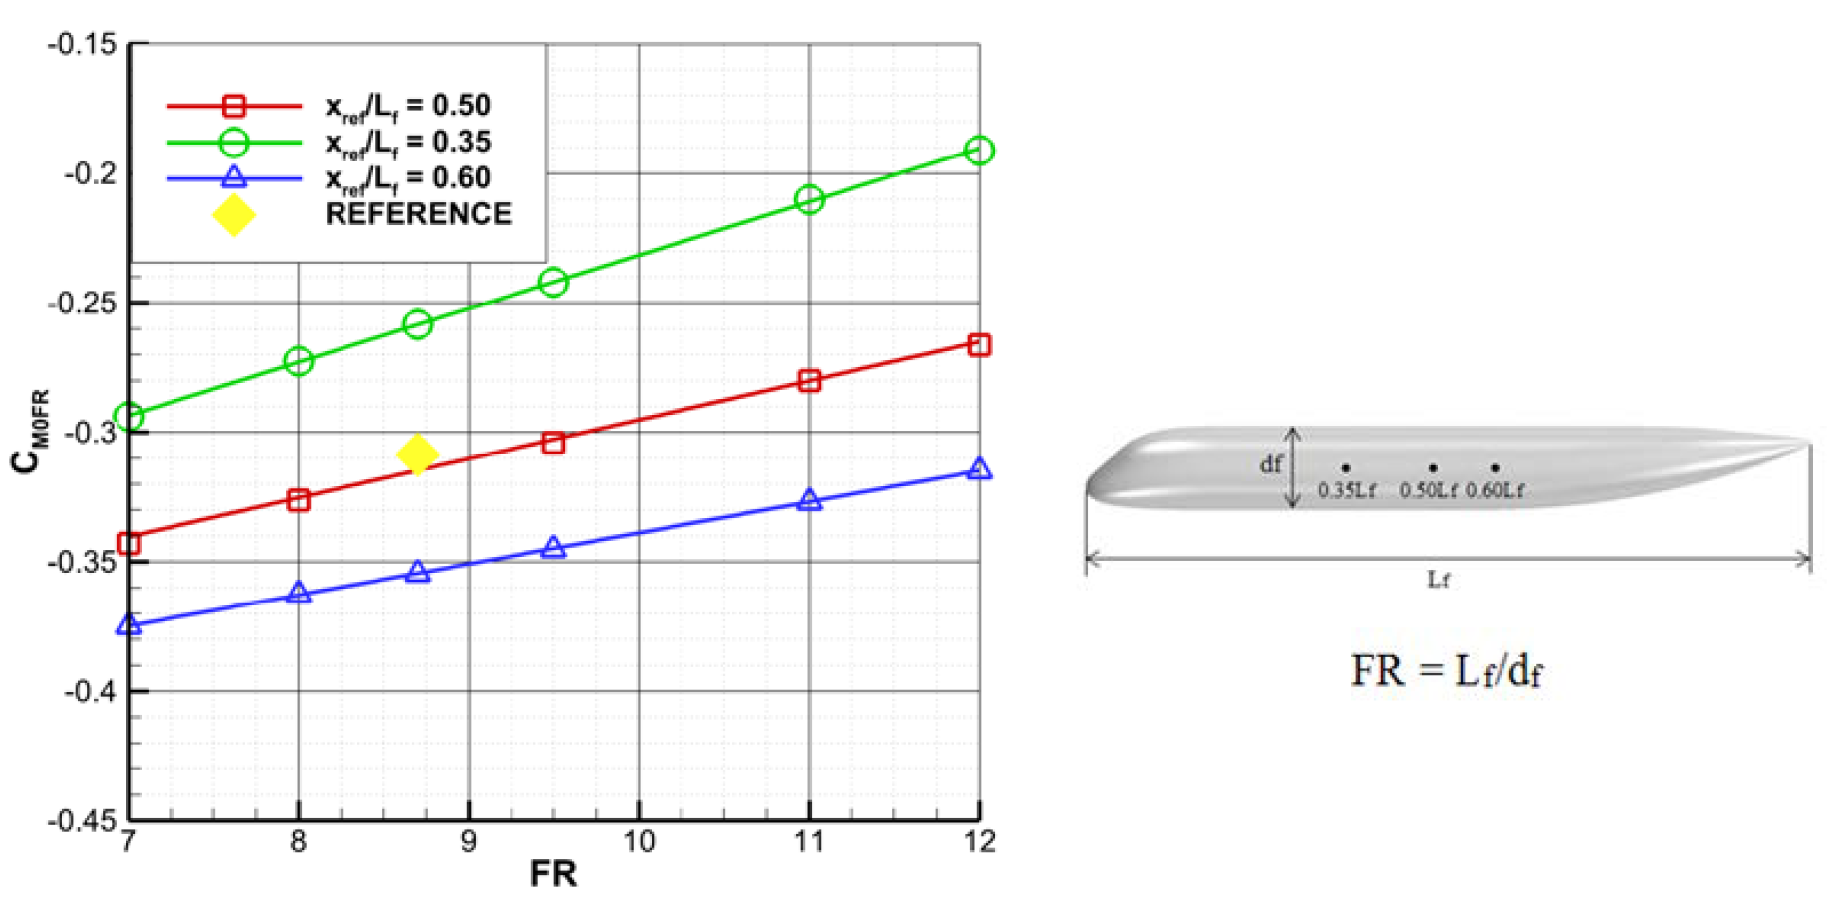
\includegraphics[height=6.4cm]{Immagini/fuselage1}
\caption{Zero angle of attack pitching moment coefficient $C_{M_{0_{FR}}}$ .}
\label{fusgeometry}
\end{figure}
\begin{figure}[H]
\centering
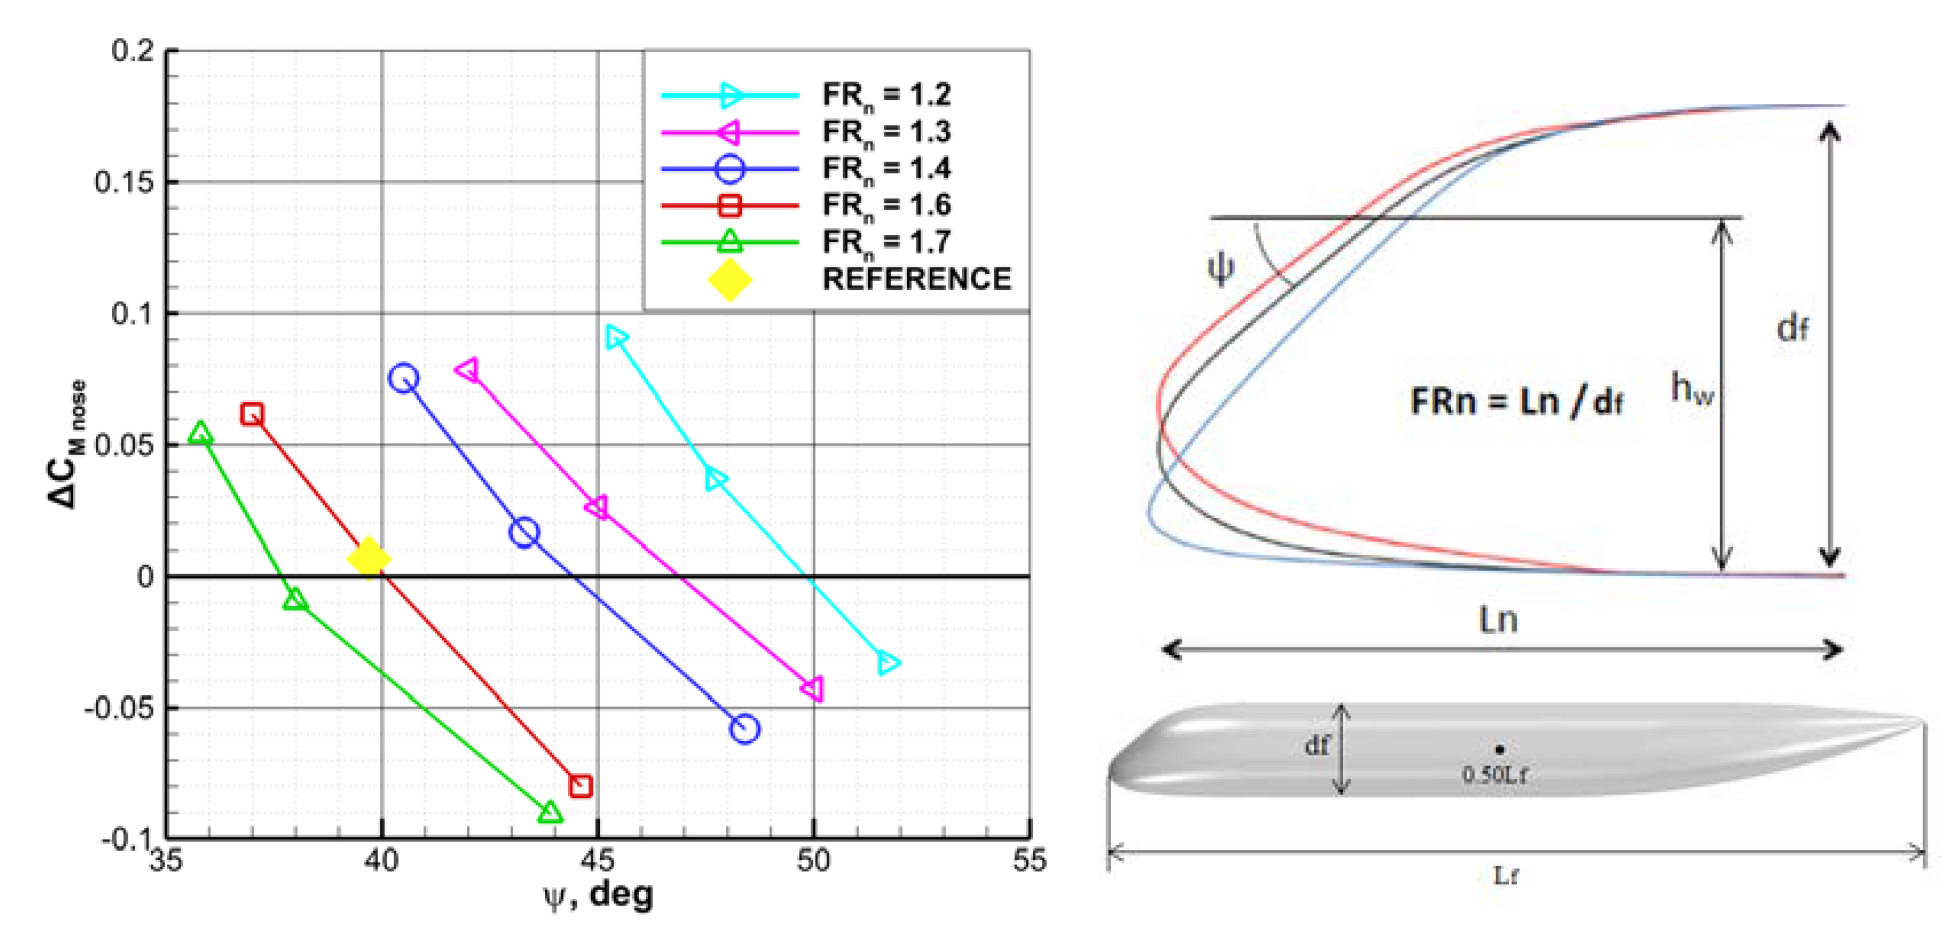
\includegraphics[height=6.4cm]{Immagini/fuselage2}
\caption{Zero angle of attack pitching moment coefficient nose correction factor.}
\label{fusgeometry}
\end{figure}
\begin{figure}[H]
\centering
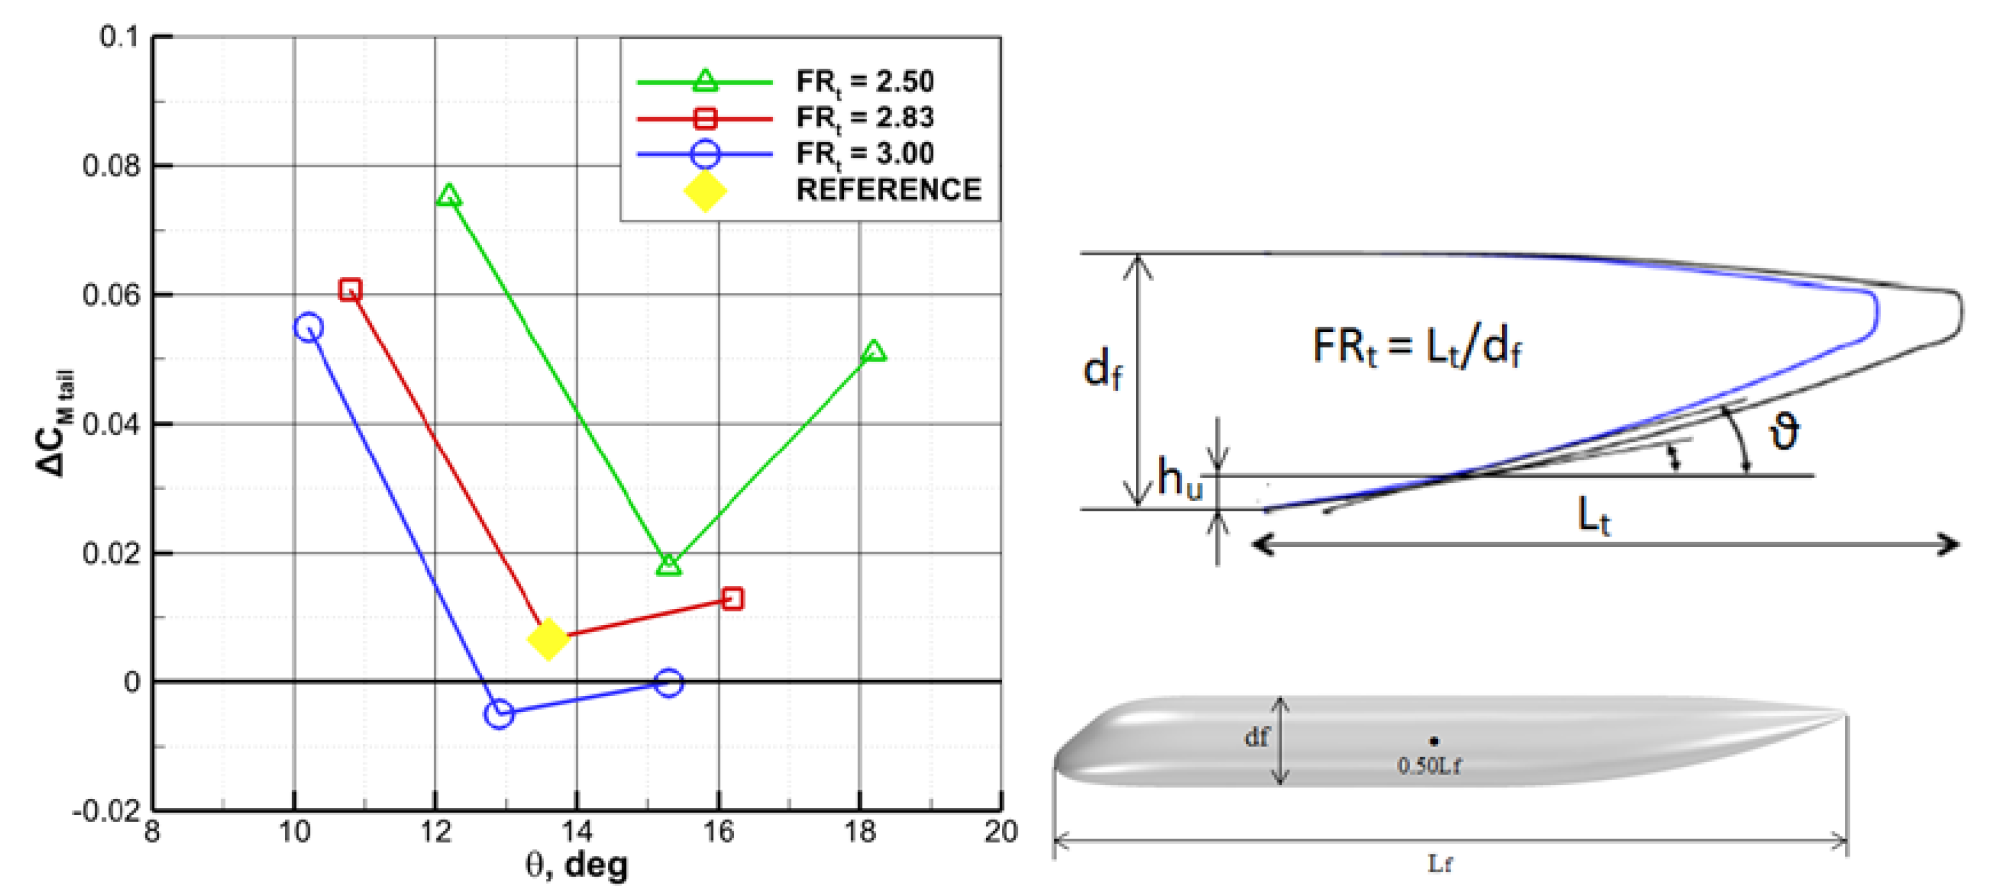
\includegraphics[height=6.4cm]{Immagini/fuselage3}
\caption{Zero angle of attack pitching moment coefficient tail correction factor.}
\label{fusgeometry}
\end{figure}
\begin{figure}[H]
\centering
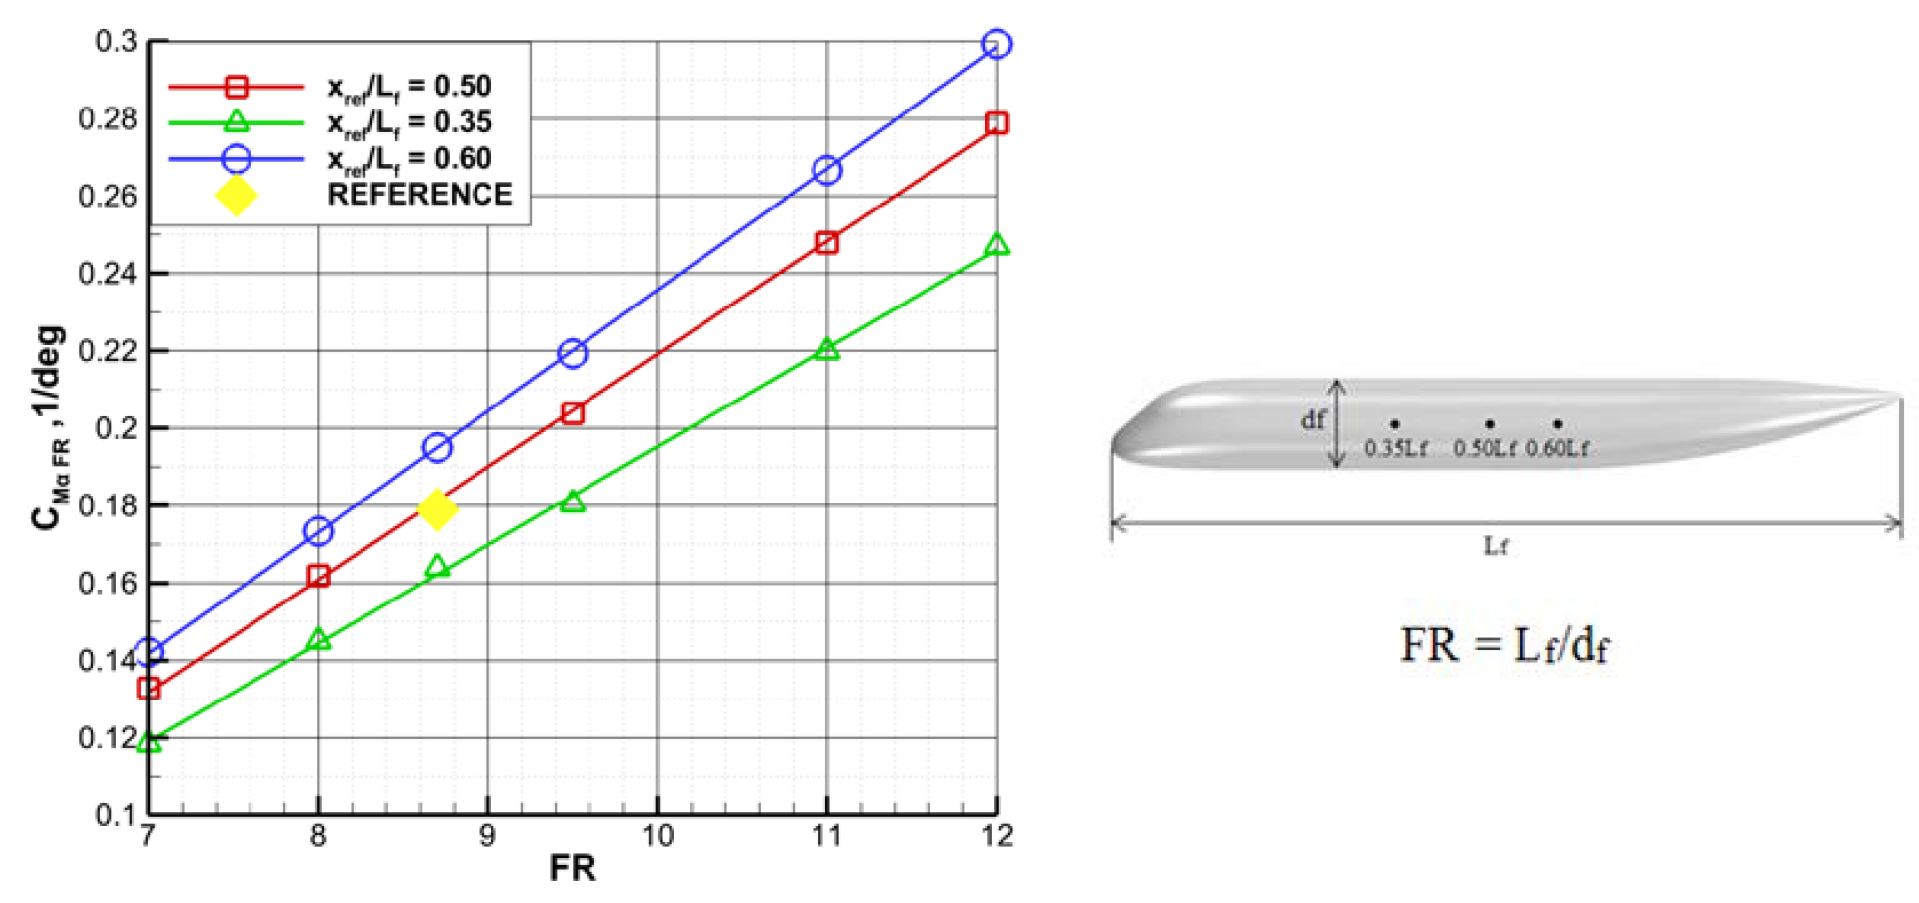
\includegraphics[height=6.4cm]{Immagini/fuselage4}
\caption{Pitching moment derivative with respect to FR.}
\label{fusgeometry}
\end{figure}
\begin{figure}[H]
\centering
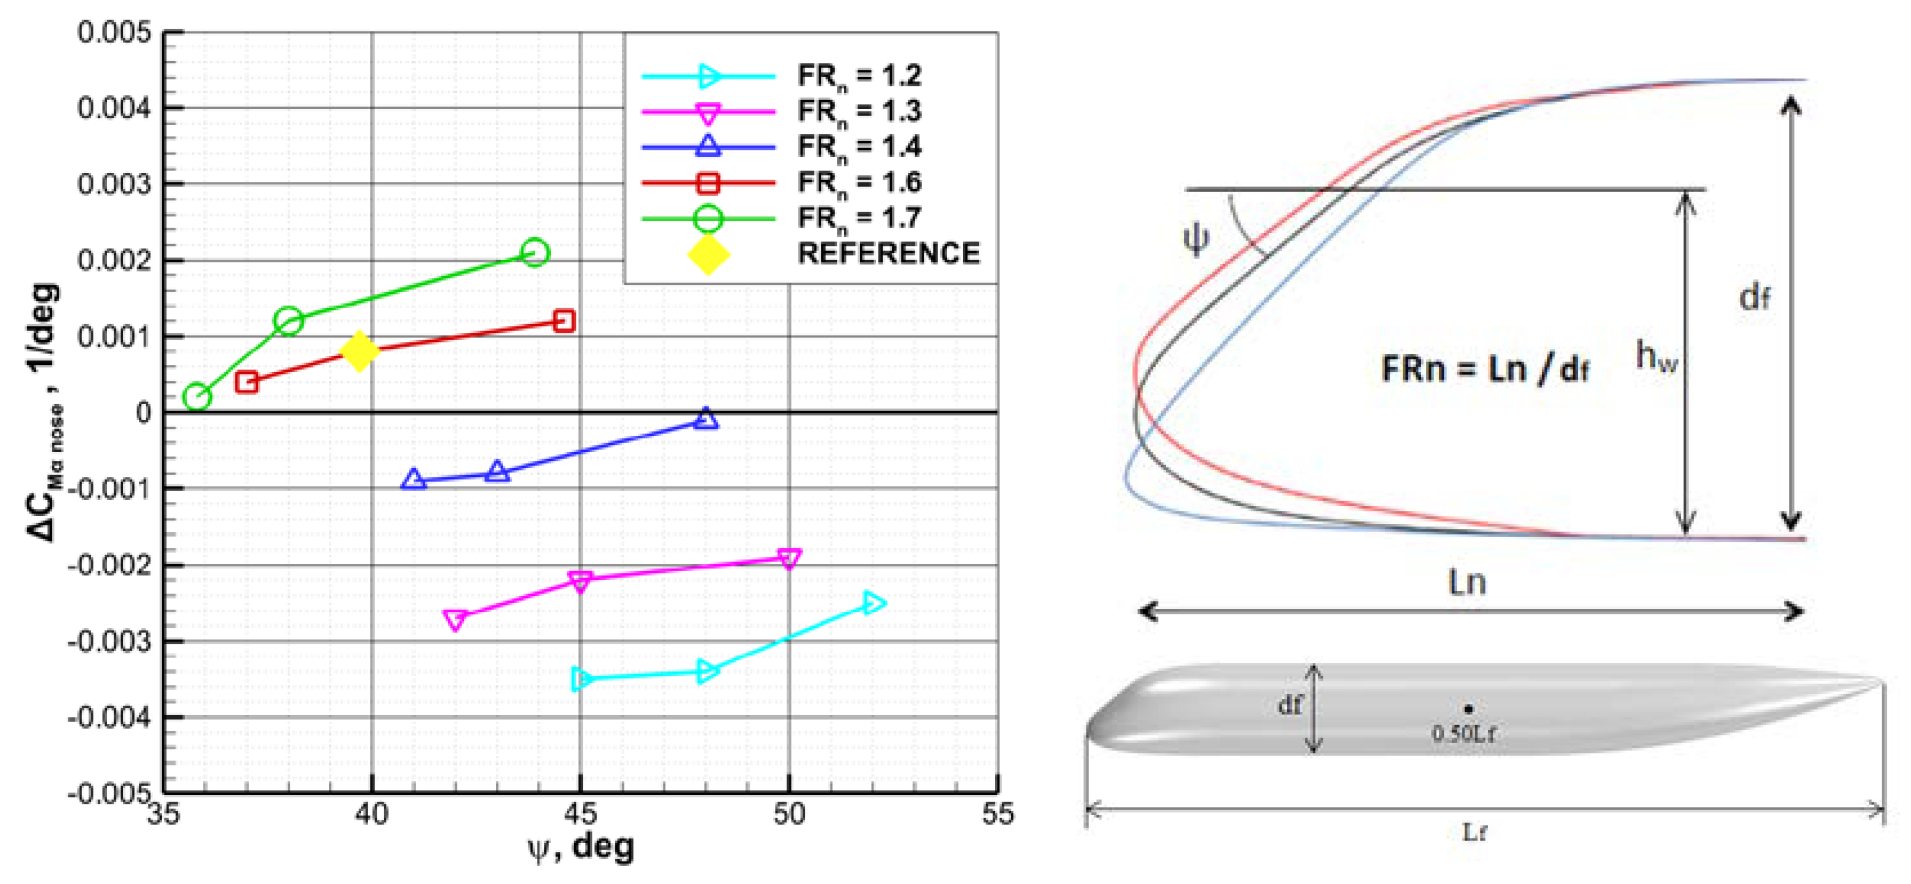
\includegraphics[height=6.4cm]{Immagini/fuselage5}
\caption{Pitching moment derivative nose correction factor.}
\label{fusgeometry}
\end{figure}
\begin{figure}[H]
\centering
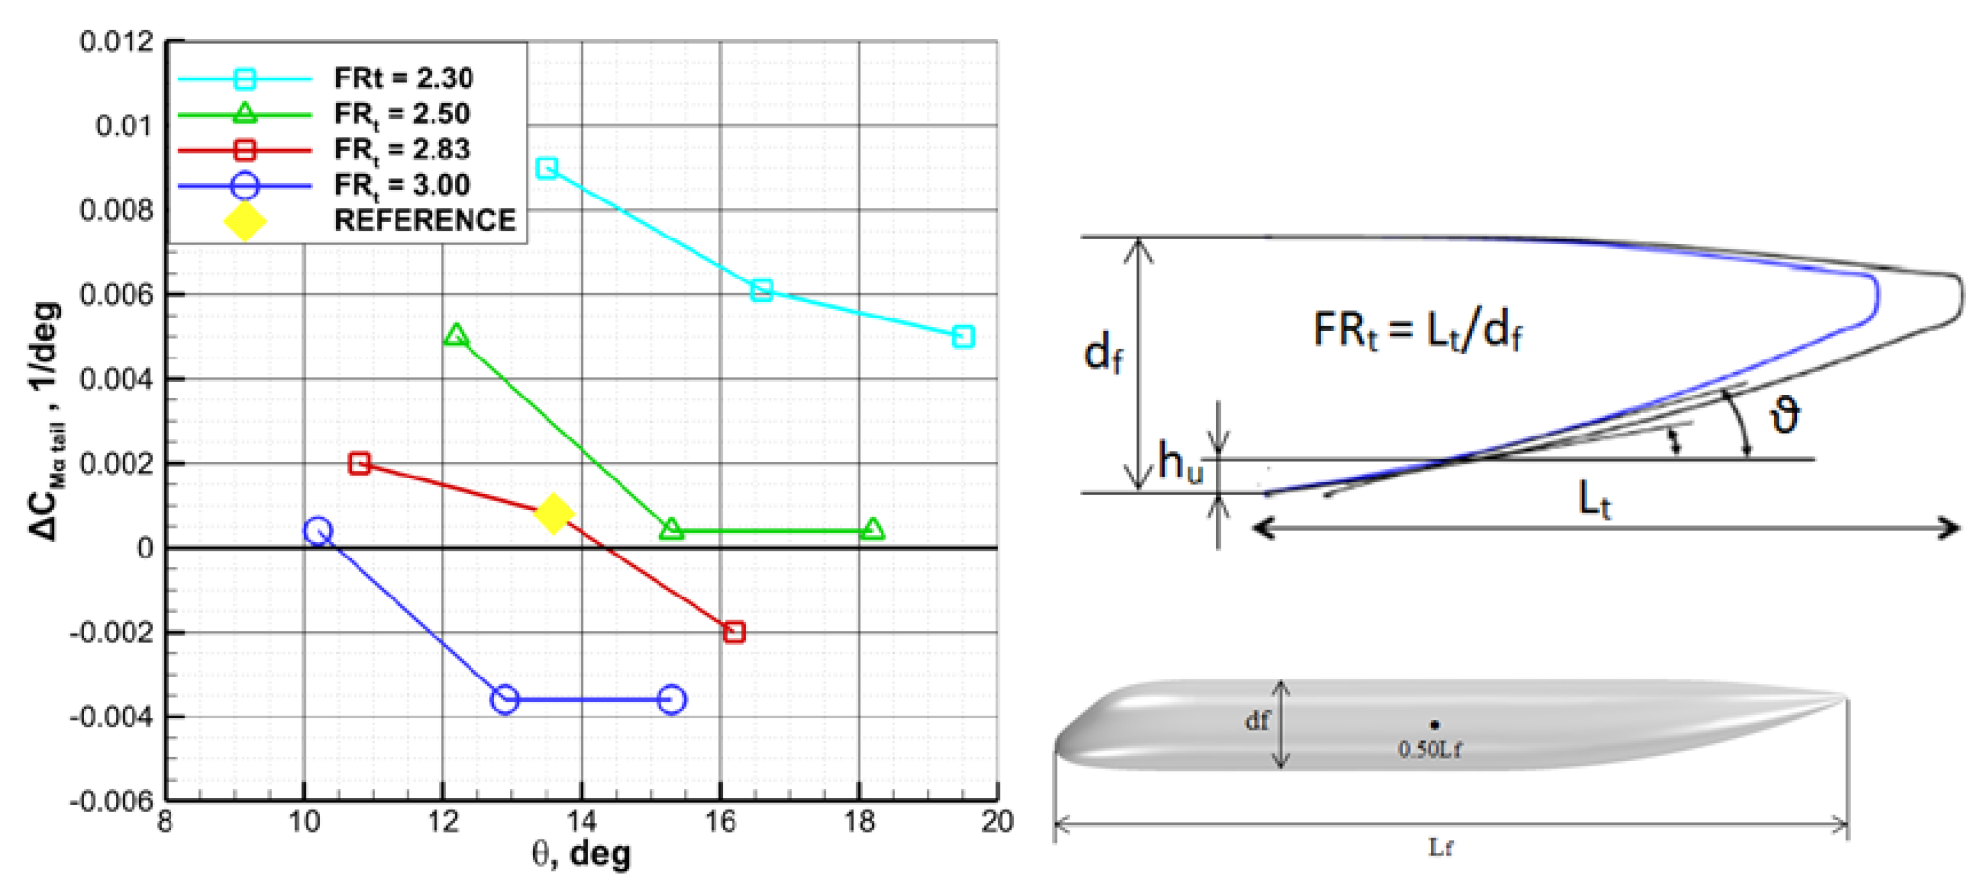
\includegraphics[height=6.4cm]{Immagini/fuselage6}
\caption{Pitching moment derivative tail correction factor.}
\label{fusgeometry}
\end{figure}


\section{Propulsors}

The effects of propeller and slipstream on airplane static longitudinal stability may be significant. It is possible to divide the power effects on longitudinal static stability in two categories: direct effects and
Indirect effects.
\subsection{Direct Effects}
 These effects are principally the following:
\begin{itemize}
\item  Effect due to the thrust and moments result from the line of action of force with respect to the CG.
\item Pitching moment due to non axial flow.
\end{itemize}

Due to these effects, the airplane pitching curve must be accounted for a change in slope $\frac{dC_m}{dC_L}$. The equations differ between turboprop engine aircraft and turbojet.\\
\\
 In case of {\bfseries turboprop} it is possible to express the power direct effects with the following equations:
\subsubsection{Pitching moment due to thrust effect}

Starting from the total lift acting on the aircraft it is possible to evaluate the dynamic pressure as follows

\begin{equation}
q = \frac{W}{S C_L}
\end{equation}

Known the dynamic pressure, the total drag is calculated

\begin{equation}
D = q S C_D
\end{equation}

Consequently it is possible to evaluate the thrust and the relative pitching moment.

\begin{equation}
C_{M_P} = \frac{T z_T}{q_{\infty} S_{ref} \bar{c}}
\end{equation}

This equation means that if the thrust acting under the cg ( $h_p > 0$ ) with increasing alpha ( and CL ) the moment coefficient undergoes a positive change, ie the power effect has an unstable contributions.

\noindent \\
\subsubsection {Pitching moment due to non axial effect}
\begin{equation}
\frac{dC_{M_P}}{dC_L} = \frac{dC_{N_P}}{d\alpha_p} \frac{S_p}{S} \frac{l_p}{\bar c} \frac{ \left ( 1 + \frac{d \epsilon}{d \alpha} \right )}{C_{L_{\alpha w}}} N_{prop}
\end{equation}

Whre $\frac{d \epsilon}{d \alpha}$ is the upwash effect forward wing, represented in fig. \ref {wingud}

\begin{figure}[H]
\centering
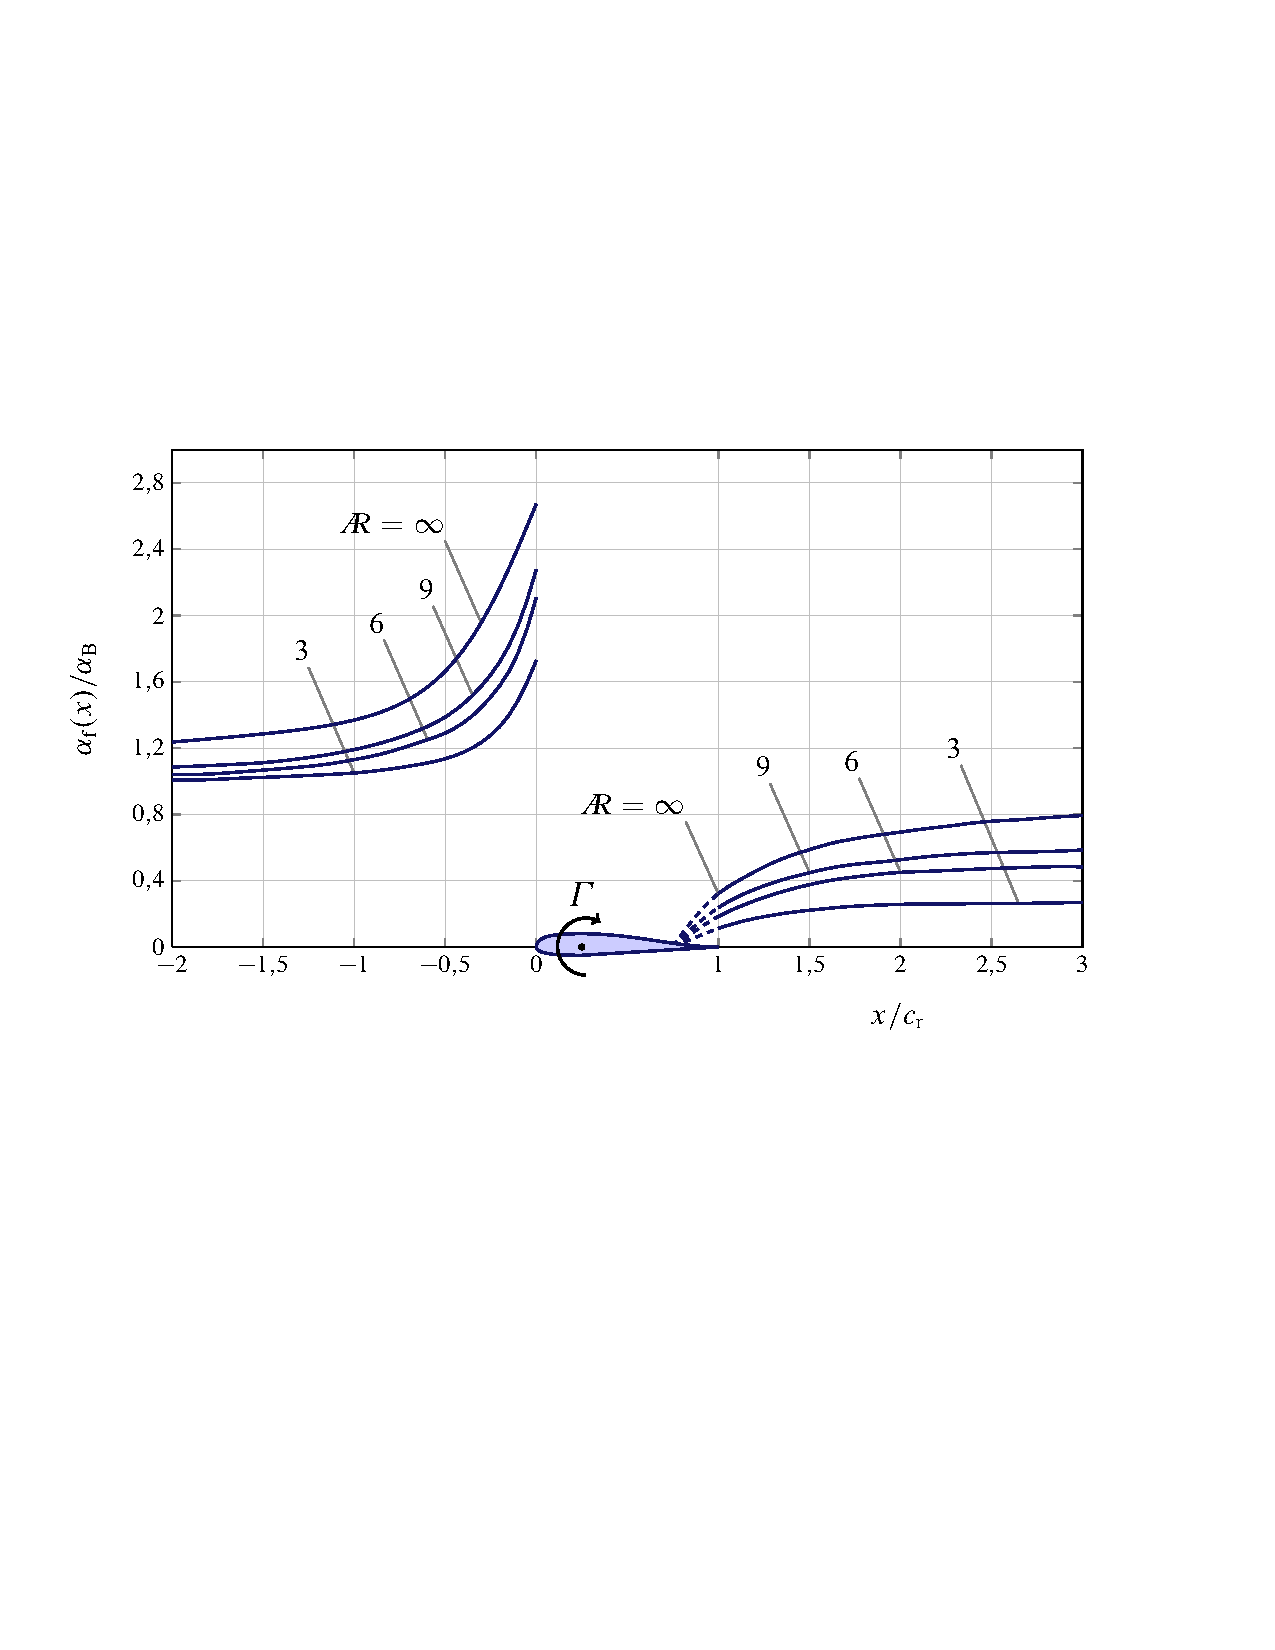
\includegraphics[height=7.3cm]{Immagini/wing_up-downwash}
\caption{Wing upwash and downwash.}
\label{wingud}
\end{figure}

%roskam 369


\section{Stability Calculation}

The forces and moments acting on an aircraft are introduced in the previous sections. In this section will be introduced the stability equation of the aircraft. Starting from the forces and the moment of single component it's possible to evaluate the moment of the aircraft. The moments are summed about the center of gravity for each aircraft.The moment or trim equations are usually placed in coefficient form by dividing through by ($q_{\infty}$ $S_{ref}$ $\bar{c}$ ), where ($q_{\infty}$ is the dynamic pressure ($\frac{1}{2} \rho v^2$ ), $S_{ref}$ is the wing reference area, and $\bar{c}$ is the mean aerodynamic chord of the wing. Now, replace the wing by its mac and locate the lift, drag, and moment of the wing at the aerodynamic center a.c.\\
Trim equation for a conventional aircraft with horizontal tail aft of the wing is

\begin{equation}
C_{M_{c.g.}} = C_N \frac{x_w}{\bar{c}} + C_C \frac{z_w}{\bar{c}} + C_{M_{a.c._{w}}} + \frac{T z_T}{q_{\infty} S_{ref} \bar{c}} - C_{L_T} \bar{V}_H \eta_T + C_{D_T} \frac{S_H}{S_w}\frac{\bar{z}_h}{\bar{c}_w} \eta_T +  C_{M_{a.c._{T}}} \eta_T \frac{S_H}{S_w}\frac{\bar{c}_h}{\bar{c}_w}
\label{eqstabilitytrim}
\end{equation}

The term $\frac{q_{{\infty}_T}}{q_{\infty}}$ is called the tail efficiency factor and comes about because of the influence of the wing on the free-stream velocity striking the tail. The tail efficiency $\eta_H$ accounts for the possibility that the horizontal tail will see a somewhat reduced velocity due to the downwash generated by the lifting wing, particularly at higher angles of attack of the wing.\cite{sforza2014commercial}. The therm $\bar{V}_H$ is the volumetric ratio and it's an important design parameter. 
\noindent \\

An aircraft must be able to stay in equilibrium for any attitude or flight condition and all thrust levels. This
requires that there be no net force or moment acting on it. The equilibrium of forces in the vertical direction is
\begin{equation}
W = L_W + L_T
\end{equation}
While to have equilibrium of moments the trim equation must be equal to zero. 
\begin{equation}
C_{M_{c.g.}} = 0
\end{equation}
The aircraft can, in general, be trimmed, that is, put into an equilibrium state where the combined lift of the wing and the tail balances the weight while the moment about the center of gravity is zero. The horizontal tail is movable, either all movable or a portion (called the elevator on an aft tail) is movable. In this way, the horizontal tail can cause the aircraft to rotate from one equilibrium (trimmed) condition to another.\cite{nicolai2010fundamentals}\\
 The aircraft is said to be statically stable if the response of the aircraft to a disturbance in angle of attack is to tend to return to the original equilibrium position.
As mentioned the criterion for static stability in an aircraft is that the derivative of $C_{M_{c.g.}}$ respect to $\alpha$ is negative. This means that if an aircraft with $CM_{\alpha} < 0 $is in equilibrium (trimmed) at a positive $\alpha$ and suddenly $\alpha$ is increased the aircraft will generate a negative moment to push the nose down toward the
original equilibrium.

\subsection{Neutral Point and Static Margin}

It is possible now to find the aerodynamic center of the aircraft, or, as it’s usually called, the neutral point, by setting the derivative of the moment coefficient with respect to angle of attack in Eq. \ref{eqstabilitytrim} equal to zero. In this case we assume the control stick is fixed so that the horizontal tail acts without any deflection of the control surface, that is, without deflecting the elevator.\\ The center of gravity location which satisfies thiscondition is called the neutral point.\\
The difference between the position of the center of gravity and the neutral point is called the static margin. It expresses how far the center of gravity of the airplane is forward of the neutral point, expressed as a fraction of the mean aerodynamic chord. The larger this quantity is, the more stable the aircraft and the less maneuverable it is. However, with greater stability the pilot workload decreases because fewer control inputs are required to keep a particular course. The airplane is said to be stiffer as the static margin increases. Typical commercial aircraft has a static margin of around $5–10\%$. When the static margin is zero the  airplane is neutrally stable, while if the static margin is negative the aircraft is statically unstable.

\subsection {Pendular Stability}

It is important to note that the horizontal component of the aerodynamic force introduces a contribute in stability equation. The arm of this force is $z_a$.\\
\begin{figure}[H]
\centering
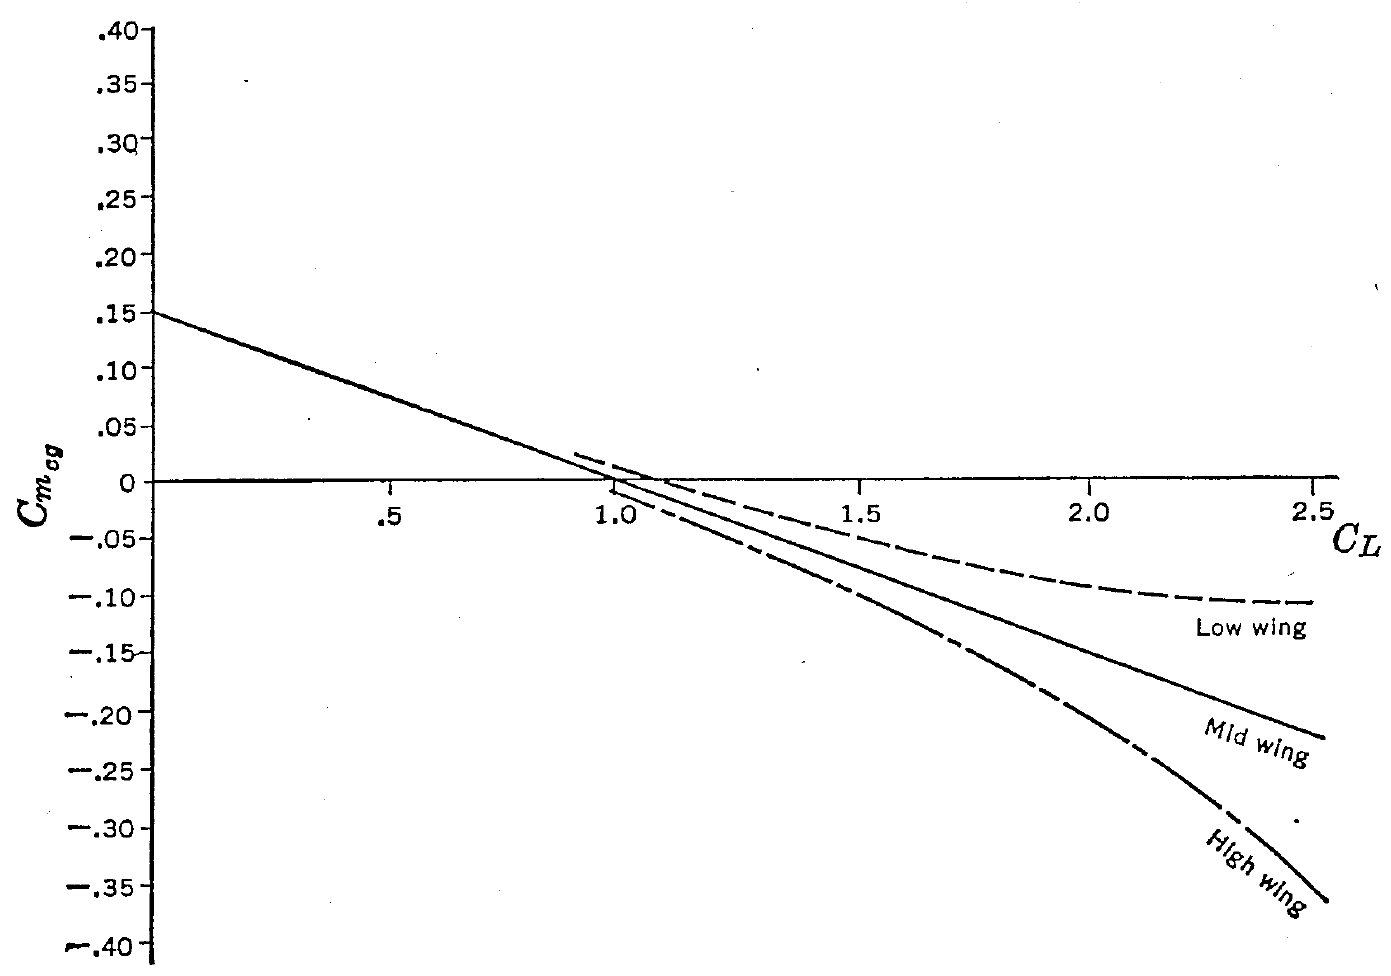
\includegraphics[height=7cm]{Immagini/pendular}
\caption{Effect of vertical location of c.g. on pitching moment.}
\label{winperkins}
\end{figure}
If the c.g. position is under the wing aerodynamic center, $z_a$ will be negative and the term will bestabilizing, whereas if the c.g. is over the wing arodynamic center, the term will be unstable. This term is usually very small with respect to the first term except at high values of the lift coefficient. \cite{PerkinsHage}
\section{Java Class Architecture}
In order to manage all required methods a manager stability class has been created, named \texttt{ACStabilityManager}. This is a complex class that defines and assigns all the useful data for the stability analysis having the operative condition as input. This class calls various method for the other class described in the previous chapter in order to evaluate the moment respect to the center of gravity of the aircraft. This moment, infact, is obtained starting from the forces acting on the aircraft's components.\\
Depending on the value of plot check the Class draws some chart useful for the knowledge of output data. 
\noindent \\

\begin{longtable} {lp{0.5\columnwidth}}
\caption{\texttt{ACStabilityManager} input variables.}
\label{tab:long}\\
\toprule
\multicolumn{1}{l}{{\bfseries Input Variable}} & \multicolumn{1}{r}{{\bfseries Description}}\\
\midrule
\endfirsthead
%
\multicolumn{2}{l}%
  {\relsize{-1}({\itshape continued from previous page})}\\
\toprule
\multicolumn{1}{l}{{\bfseries Input Variable}} & \multicolumn{1}{r}{{\bfseries Description}}\\
\endhead
%
\midrule \multicolumn{2}{r}{{\relsize{-1}\itshape continued on next page}}\\
\endfoot
%
\bottomrule
\endlastfoot
%
		\toprule
		\lstinline[language=Java]!Aircraft! - the Aircraft & The object of analysis.\\ \hline 
		\lstinline[language=Java]!MyAirfoil! - Mean Airfoil & In order to make computing faster the mean airfoil is calculated in the test class. \\ \hline 
		\lstinline[language=Java]!ConditionEnum! - the Operative Condition &  In JPAD is defined an enumeration of operating condition: TAKE-OFF, CRUISE and LANDING. Giving the condition as input, the builder of the stability manager automatically calculates all the parameters (such as Mach number or high-lift devices deflection). \\ \hline 
		\lstinline[language=Java]!Amount<Angle>! - alpha Min, alpha Max & These are the first and the last value of the $\alpha_b$ array for witch will be made the analysis. They can to be in degree or radian. These values may to be null in order to execute analysis only for an angle of attack. In this case the values of alpha max and alpha min wil be alpha body $\pm 1^{\circ}$. It's possible to set the number of values with a setter.\\ \hline 
		\lstinline[language=Java]!Amount<Angle>! - alpha Body & Is the angle of attack (alpha body) for the calculation of numerical value of CL, CD, CM. This value may be null. In this case the class calculates only all stability characteristics at an array of alpha body\\ \hline 
		\lstinline[language=Java]!boolean! - plot Check & This is a check value in order to make charts or not.\\ \hline 
		\lstinline[language=Java]!String! - subfolder Path & This is the folder path where the charts will be saved.\\ \hline 
		\lstinline[language=Java]!String! -path XML HighLift & This is the path of the input file for high-lift data in take off condition or landing.\\ \hline 
		\bottomrule
\end{longtable}


The class \texttt{ACStabilityManager} contains different methods in order to evaluate Lift, Drag and Moments contributes. All methods and related functionality are expressed in the following table.

\begin{longtable} {lp{0.5\columnwidth}}
\caption{Methods of the class \texttt{ACStabilityManager}.}
\label{tab:long}\\
\toprule
\multicolumn{1}{l}{{\bfseries Method }} & \multicolumn{1}{r}{{\bfseries Description}}\\
\midrule
\endfirsthead
%
\multicolumn{2}{l}%
  {\relsize{-1}({\itshape continued from previous page})}\\
\toprule
\multicolumn{1}{l}{{\bfseries Method}} & \multicolumn{1}{r}{{\bfseries Description}}\\
\endhead
%
\midrule \multicolumn{2}{r}{{\relsize{-1}\itshape continued on next page}}\\
\endfoot
%
\bottomrule
\endlastfoot
%
		\toprule
		\lstinline[language=Java]!ACStabilityManager!& It is the builder of the class. It initialize all useful data\\ \hline 
		\lstinline[language=Java]!calculateAll! & This method call all the other methods of the class in ordet to valculate lift, drag and pitching moment characteristics of the component. \\ \hline 
		\lstinline[language=Java]!calculateLiftCharacteristics()!& This method call the methods related to the lift calculation that fill the array and, eventually, produce charts.\\ \hline 
		\lstinline[language=Java]!calculateDragCharacteristics()! &  The same of previous for drag.\\ \hline 
		\lstinline[language=Java]!calculateMomentCharacteristics()!  & The same of previous for pitching moment.\\ \hline 
		\lstinline[language=Java]!calculateWingLiftCharacteristics()!  & This method uses methods of lift calculation classes in order to fill the lift arrays for wing both in cruise and in take off or landing.\\ \hline
		\lstinline[language=Java]!calculateHTailLiftCharacteristics()!  & This method uses methods of lift calculation classes in order to fill the lift arrays for wing both in cruise and in take off or landing.\\ \hline
		\lstinline[language=Java]!calculateFuselageLiftCharacteristics()!  & This method uses methods of lift calculation classes in order to correct the lift coefficient of an isolated wing.\\ \hline 
		\lstinline[language=Java]!calculateWingDragCharacteristics! & This method uses methods of lift calculation classes in order to fill the lift arrays for wing both in cruise and in take off or landing.\\\hline 
		\lstinline[language=Java]!calculateHTailDragCHaracteristics! & The same of previous for horizontal tail. This method consider also the elevator deflections.\\\hline 
		\lstinline[language=Java]!calculateWingMomentCharacteristics()!& This method call the methods related to the pitching moment calculation that fill the array and, eventually, produce charts.\\ \hline \\
		\lstinline[language=Java]!calculateHTailMomentCharacteristics()!& The same of previous for horizontal tail.\\ \hline 
		\lstinline[language=Java]!calculateFuselageMomentCharacteristics()!& The same of previous for fuselage.\\ \hline 
		\lstinline[language=Java]!calculatePowerEfects!& This method introduces power effect on the stability.\\ \hline
		\lstinline[language=Java]!deltaEElevatorCalculator!& This method calculates the deflection of the elevator at alpha.\\ \hline 
		\lstinline[language=Java]!calculateMoment()!& This method calculates the pitching moment of the entire aircraft respect to the center of gravity.\\ \hline 
		\lstinline[language=Java]!calculatedeltaEEquilibrium()!& This method calculates the angle of deflection of the horizontal tail for the trim..\\ \hline 
		\lstinline[language=Java]!neutralPointCalculator!& This method calculates the neutral point and eventually draws the charts.\\ \hline 
		\bottomrule
	\end{longtable}

\begin{center}
	\captionof{table}{Output charts for the class \texttt{ACStabilityManager}.}
	\begin{tabular}{| l | l | l |}
		\hline
		&  Cl vs $\alpha$ - airfoils.\\ 
		&CL vs $\alpha_w$ - wing.\\ 
		& Stall path - wing.\\  
		&CD parasite vs $\alpha_w$ - wing.\\  
		&CD induced vs $\alpha_w$ - wing.\\ 
		&CD total vs $\alpha_w$ - wing.\\  
		&CL vs $\alpha_h$ - horizontal Tail. With elevator deflections.\\ 
		&CD total vs $\alpha_h$ - horizontal Tail. With elevator deflections.\\ 
		&Stall path - horizontal Tail.\\ 
		{\bfseries Clean}		 &CL vs $\alpha_w$ - wing-body.\\  
		&CL vs $\alpha_w$ - Total. With elevator Deflection.\\  
		&Downwash gradient vs $\alpha_b$ - linear and non-linear.\\  
		&Downwash angle vs $\alpha_b$ - linear and non-linear.\\ 
		&Cm vs $\alpha\_b$ - respect to c/4 of MAC for wing. \\  
		&Cm vs $\alpha\_b$ - respect to ac for wing. \\
		&Cm vs $\alpha\_b$ - respect to c/4 of MAC for horizontal Tail. \\ \
		&Cm vs $\alpha\_b$ - respect to ac for horizontal Tail. \\ 
		&Cm vs $\alpha\_b$ - for fuselage. \\ 
		&Cm vs $\alpha\_b$ - respect to cg for aircraft. With elevator deflections. \\ 
		&Cm vs $\alpha\_b$ - respect to ac for wing. \\ 
		& $\delta_{ee}$ vs $\alpha\_b$  \\ 
		& Neutral Point vs $C_{L_{tot}}$  \\ \hline 	
		&	 The same for cruise \\ 	
		{\bfseries Take Off -  Landing}	 	& CL vs $\alpha_w$ - wing. Whith High Lift devices effects. \\ 
		&	 CD total vs $\alpha_w$ - wing. With high lift devices effects.\\ \hline   
		\hline
	\end{tabular}
\end{center}

\subsection{Focus on the class methods}
The first method of the class is the builder. An important function is carried out by this method that assigns all the useful data. The main purposes of the builder are the following

\begin{enumerate}
	\item An array of $\alpha_b$ is defined . This is an array of nValue in Deg. The number of elements is settable by the user.
	\item According to the condition it sets the Mach number. The Cruise, take Off and Landing Mach numbers are defined in the aircraft aerodynamic manager \texttt{ACAerodynamicManager}. In this way it's possible to access to the value from the aircraft object.
	\item The operating condition (such as altitude and Mach number) are defined according to the flight condition.
	\item The center of gravity is defined starting from the correct weight of the aircraft. In particular:
	\begin{itemize}
		\item Take Off $\rightarrow$ MTOW
		\item Cruise $\rightarrow$ $\frac{(MTOW + MZFW)}{2}$
		\item Landing $\rightarrow$  MZFW
	\end{itemize}
\end{enumerate}



 All the other methods are structured in order to obtain the following results:
\begin{enumerate}
	\item Array filling
	\item Value at $\alpha_b$
	\item Charts
\end{enumerate}
\begin{figure}[H]
	\centering
	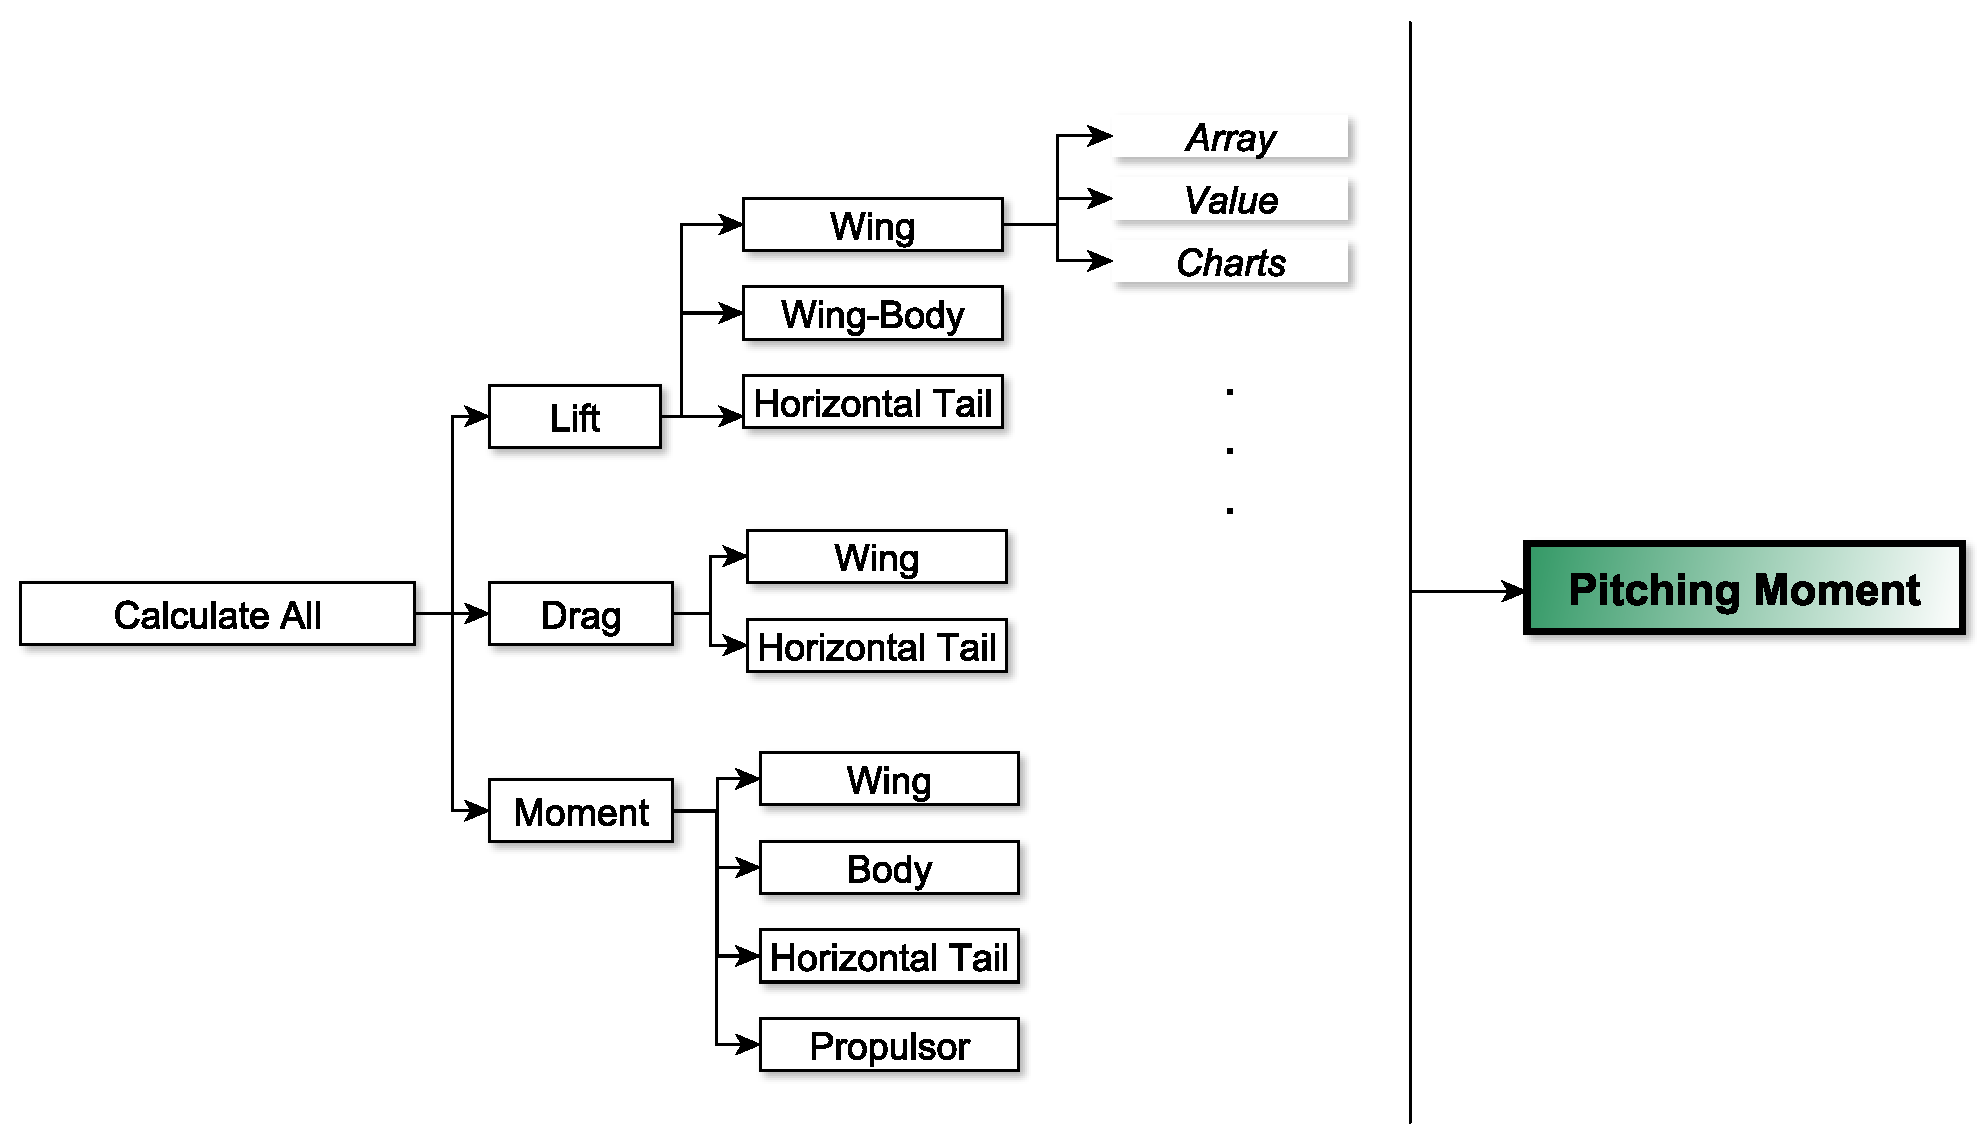
\includegraphics[height=8.3cm]{Immagini/acclass}
	\caption{Methods in ACStabilityManager class.}
	\label{acc}
\end{figure}


The value for the $\alpha_b$ array are saved in array which can be read via getter methods.

\begin{lstlisting}[frame=rbl,caption={{\footnotesize Some of Output Array}},label= [style=\bfseries]{Listing}]

 //Output Arrays // Correspond to alpha body array
 
private double [] cLWingCleanArray;
private double [] cLWingTOArray;
private double [] cLWingLandingArray;
private double [] cLWingBodyArray;
private double [] cLAlphaArray;
private double [] cLHTailCleanArray;
private Double [] downwashAnglesArray;
private double [] tauIndexArray = new double [deltaEArray.length];
private double [] cLCompleteAircraftdeltaEArray = new double [deltaEArray.length];

private double [] parasiteCDWingCleanArray;
private double [] parasiteCDHTailCleanArray;
private double [] inducedCDWingArray;
private double [] inducedCDHTailArray;
private double [] cDWingCleanArray;
\end{lstlisting}


The results for the horizontal tail are obtained for an array of elevator deflections which value can be set by the user. Consequently the resultant values for the horizontal tail are organized in a Map.


%spiega la classse per il calcolo del cl del piano di coda con deflessione dell'equilibratore ( vedi doc di calculateCLWithElevatorDeflection in lsaerodynamic manager)
%
%		// The calculation of the lift coefficient with a deflection of the elevator is made by the
%		// method calculateCLWithElevatorDeflection. This method fills the array of 20 value of CL in
%		// its linear trait. 
%		// The procedure used to calculate the CL is the following. It's important to know that 
%		// it's necessary to call the method nasaBlackwellCompleteCurve in order to obtain the
%		// cl linear slope of the horizontal tail with no elevator deflection.
%		//
%		//1 . First of all the tau factor it's calculated used the method calculateTauIndex in the .. class
%		//2. It's necessary to get the linear slope of the horizontal tail with no elevator defletion.
%		// 3. The alphazero lift of the deflected configuration is calculated with this formula
%		//   alphaw= tau per delta e
%		// 4. At this point it's possible to create an alpha array, starting from the alpha zero lift, until
%		//   15 degrees after.
%		// 5. the value of cl for each alpha is calculated with the formula :
%		//  cl alfa * (alfa + t delta e)

% intro
% riepilogo di tutte le classi in schema. vedi su quaderno  prima di stabilita
% schema in yed
 % per l' ala scrivi le grandezze geometriche con foto
 
\section{Case Study}
Several graps used in this modulus are presented in previous chapter. So, following, there will be only the new results.

\subsection{ATR 72}

\begin{figure}[H]
\centering
% Moment Coefficient vs alpha for Wing respect to A C 
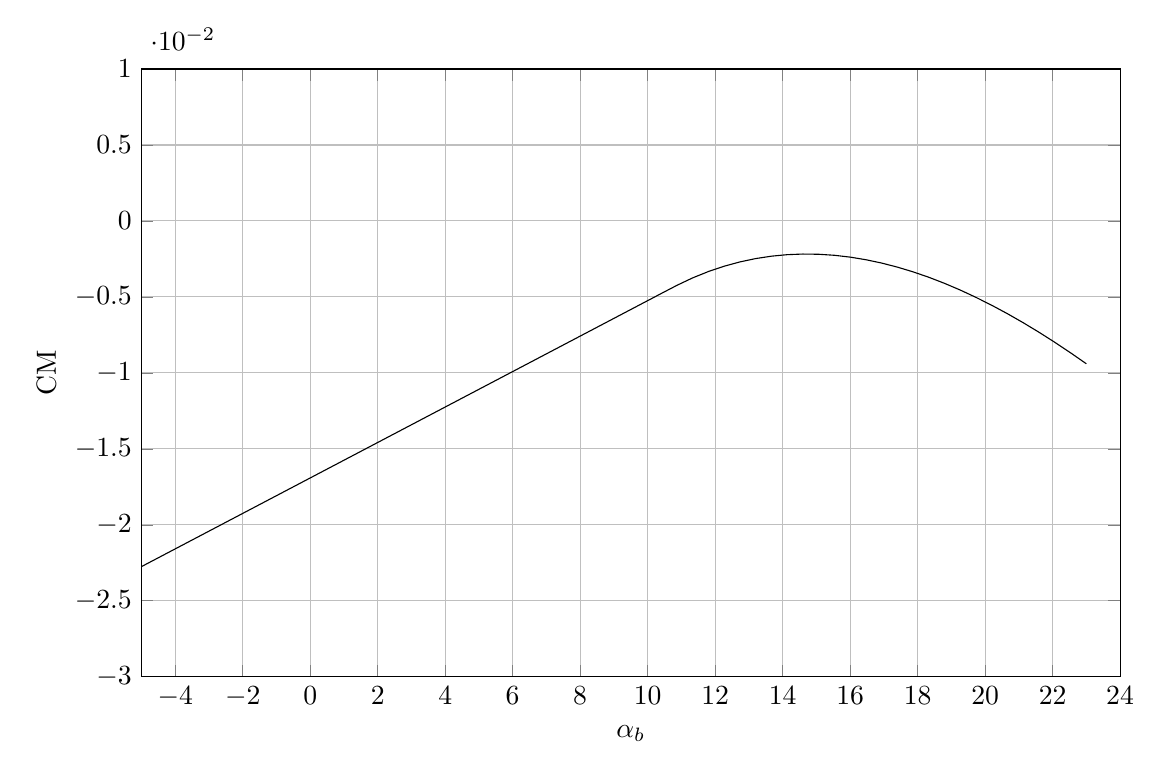
\begin{tikzpicture}

\begin{axis}[
width=14.01cm,
height=9.3cm,
xmin=-5,
xmax=24,
xlabel={$\alpha_b$},
xmajorgrids,
ymin=-0.03,
ymax=0.01,
ylabel={CM},
ymajorgrids,
]
\addplot [
color=black,
solid
]
table[row sep=crcr]{
-4.999999999999999	-0.022752300258962188\\
-4.533333333333332	-0.02220771010412249\\
-4.0666666666666655	-0.021663119949282827\\
-3.5999999999999988	-0.021118529794443147\\
-3.133333333333332	-0.02057393963960345\\
-2.666666666666665	-0.020029349484763755\\
-2.1999999999999984	-0.01948475932992409\\
-1.7333333333333318	-0.018940169175084412\\
-1.2666666666666653	-0.01839557902024472\\
-0.7999999999999987	-0.01785098886540504\\
-0.33333333333333215	-0.017306398710565357\\
0.13333333333333441	-0.01676180855572568\\
0.600000000000001	-0.016217218400886\\
1.0666666666666675	-0.015672628905666897\\
1.533333333333334	-0.01512803878136793\\
2.000000000000001	-0.014583448657068968\\
2.4666666666666677	-0.014038858532770001\\
2.9333333333333345	-0.013494268408471033\\
3.4000000000000012	-0.012949697581426329\\
3.866666666666668	-0.012405108169835853\\
4.333333333333335	-0.011860518758245375\\
4.800000000000002	-0.011315929346654896\\
5.266666666666668	-0.010771339935064425\\
5.733333333333335	-0.010226750523473951\\
6.200000000000002	-0.009682161111883468\\
6.666666666666669	-0.009137571700293\\
7.1333333333333355	-0.008592982288702514\\
7.600000000000002	-0.008048392877112042\\
8.066666666666668	-0.007503803465521576\\
8.533333333333335	-0.006959214053931069\\
9.000000000000002	-0.006414624642340602\\
9.466666666666669	-0.005870035230750119\\
9.933333333333335	-0.0053254458191596575\\
10.400000000000002	-0.004780826419687604\\
10.866666666666669	-0.004240981279897541\\
11.333333333333336	-0.0037500920749439434\\
11.800000000000002	-0.0033314180543403734\\
12.26666666666667	-0.0029820111695065717\\
12.733333333333336	-0.002698753776889693\\
13.200000000000003	-0.002479114588805469\\
13.66666666666667	-0.0023209127078930984\\
14.133333333333336	-0.002221863657197933\\
14.600000000000003	-0.002180395445745009\\
15.06666666666667	-0.0021944710591490888\\
15.533333333333337	-0.0022622544080148827\\
16.000000000000004	-0.002382431676358512\\
16.46666666666667	-0.0025534662225705244\\
16.933333333333334	-0.002773199046169686\\
17.4	-0.003040193926269407\\
17.866666666666664	-0.00335309079848985\\
18.33333333333333	-0.0037105295984510137\\
18.799999999999994	-0.004111150261773044\\
19.26666666666666	-0.004553442702549079\\
19.733333333333324	-0.005035428278751983\\
20.19999999999999	-0.00555565320076135\\
20.666666666666654	-0.0061127267455573465\\
21.13333333333332	-0.006705258190119817\\
21.599999999999984	-0.0073318568114288316\\
22.06666666666665	-0.007991131886464406\\
22.533333333333314	-0.008681692692206559\\
22.999999999999993	-0.009402148505635257\\
};
\end{axis}
\end{tikzpicture}%

\caption{ATR 72 . Mach 0.45. Pitching Moment Coefficient of the Wing respect to a quarter of MAC.}
\label{fig:stallATR}
\end{figure}
\noindent\\
\begin{figure}[H]
\centering
% Moment Coefficient vs alpha for Wing respect to A C 
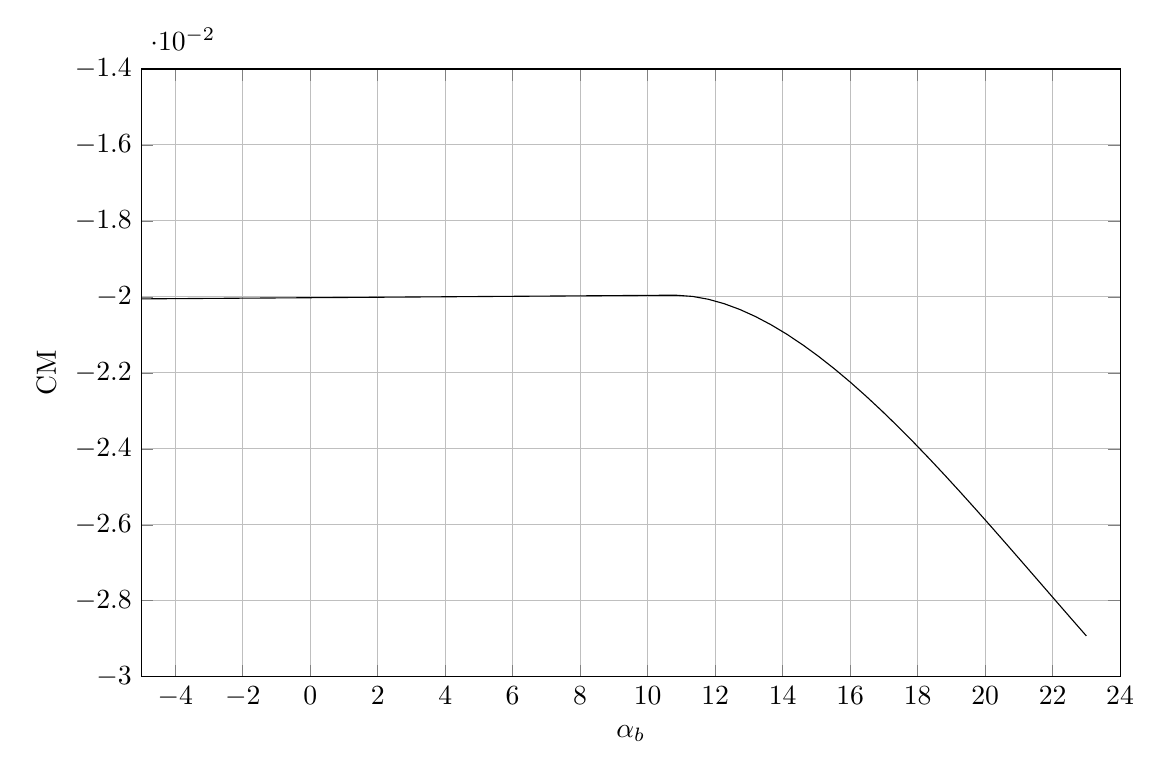
\begin{tikzpicture}

\begin{axis}[
width=14.01cm,
height=9.3cm,
xmin=-5,
xmax=24,
xlabel={$\alpha_b$},
xmajorgrids,
ymin=-0.03,
ymax=-0.014,
ylabel={CM},
ymajorgrids,
]
\addplot [
color=black,
solid
]
table[row sep=crcr]{
-4.999999999999999	-0.020052350355747508\\
-4.533333333333332	-0.020049490164630493\\
-4.0666666666666655	-0.020046629973513478\\
-3.5999999999999988	-0.020043769782396463\\
-3.133333333333332	-0.02004090959127947\\
-2.666666666666665	-0.020038049400162464\\
-2.1999999999999984	-0.02003518920904543\\
-1.7333333333333318	-0.020032329017928428\\
-1.2666666666666653	-0.020029468826811427\\
-0.7999999999999987	-0.02002660863569439\\
-0.33333333333333215	-0.020023748444577393\\
0.13333333333333441	-0.020020888253460375\\
0.600000000000001	-0.020018028062343377\\
1.0666666666666675	-0.02001518514796535\\
1.533333333333334	-0.020012325811887537\\
2.000000000000001	-0.02000946647580974\\
2.4666666666666677	-0.020006607139731937\\
2.9333333333333345	-0.020003747803654142\\
3.4000000000000012	-0.02000088846757634\\
3.866666666666668	-0.019998029131498538\\
4.333333333333335	-0.01999516979542074\\
4.800000000000002	-0.01999231045934294\\
5.266666666666668	-0.01998945112326514\\
5.733333333333335	-0.019986591787187345\\
6.200000000000002	-0.01998373245110954\\
6.666666666666669	-0.019980873115031734\\
7.1333333333333355	-0.01997801377895393\\
7.600000000000002	-0.019975154442876137\\
8.066666666666668	-0.019972295106798345\\
8.533333333333335	-0.019969435770720523\\
9.000000000000002	-0.019966576434642735\\
9.466666666666669	-0.01996371709856493\\
9.933333333333335	-0.019960857762487134\\
10.400000000000002	-0.019957998426409326\\
10.866666666666669	-0.019957917611308103\\
11.333333333333336	-0.01998813389905404\\
11.800000000000002	-0.02006303628996213\\
12.26666666666667	-0.02017880976789285\\
12.733333333333336	-0.020331904703815955\\
13.200000000000003	-0.02051947356199313\\
13.66666666666667	-0.02073907996389296\\
14.133333333333336	-0.020988177980988346\\
14.600000000000003	-0.021265033519538703\\
15.06666666666667	-0.021567388422336464\\
15.533333333333337	-0.021893211954119002\\
16.000000000000004	-0.022241064527768303\\
16.46666666666667	-0.022609256043377796\\
16.933333333333334	-0.022995396711066596\\
17.4	-0.023397909329412176\\
17.866666666666664	-0.023815302316313253\\
18.33333333333333	-0.02424608408966859\\
18.799999999999994	-0.024688763067376936\\
19.26666666666666	-0.02514167994151198\\
19.733333333333324	-0.0256026515529142\\
20.19999999999999	-0.02607008153356528\\
20.666666666666654	-0.026542444024645076\\
21.13333333333332	-0.027018213167333466\\
21.599999999999984	-0.027495863102810325\\
22.06666666666665	-0.02797386797225554\\
22.533333333333314	-0.028450701916848967\\
22.999999999999993	-0.028924839077770565\\
};
\end{axis}
\end{tikzpicture}%

\caption{ATR 72 . Mach 0.45. Pitching Moment Coefficient of the Wing respect to AC. AC=0.2374 implemented method. AC= 0.24445 DeYoung Harper.}
\label{fig:stallATR}
\end{figure}
\begin{figure}[H]
\centering
% Moment Coefficient vs alpha for Wing respect to A C 
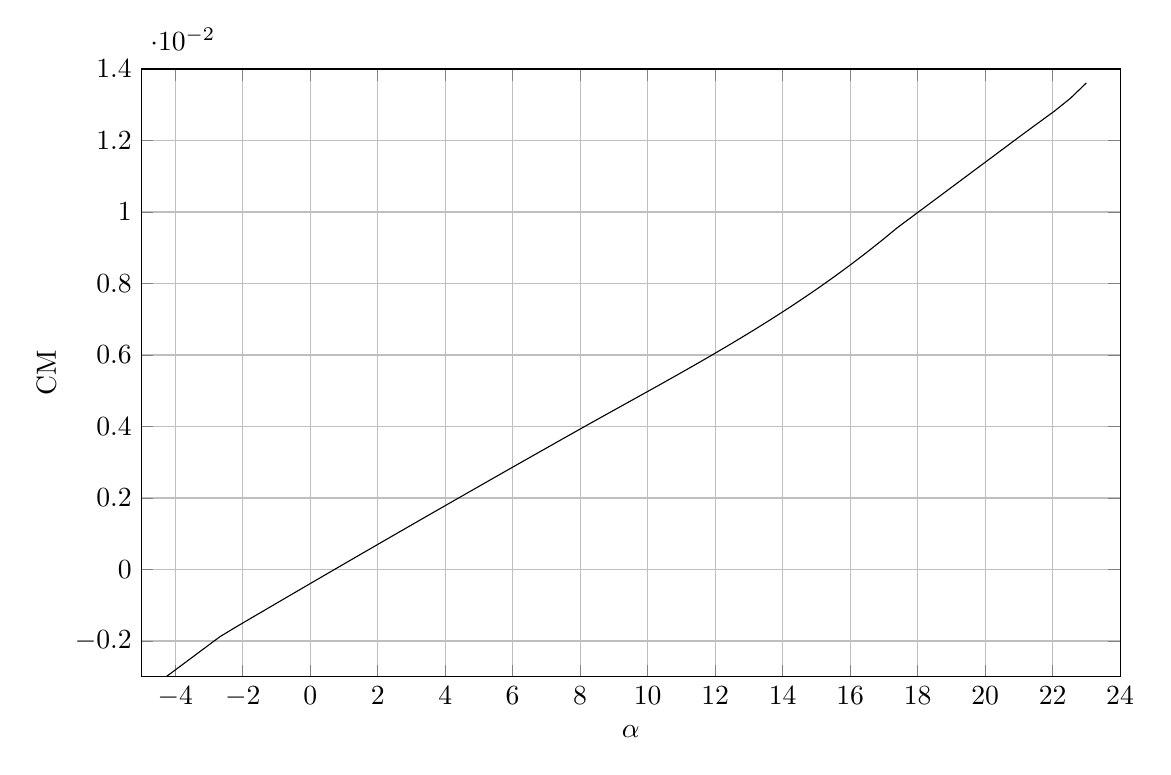
\begin{tikzpicture}

\begin{axis}[
width=14.01cm,
height=9.3cm,
xmin=-5,
xmax=24,
xlabel={$\alpha$},
xmajorgrids,
ymin=-0.003,
ymax=0.014,
ylabel={CM},
ymajorgrids,
]
\addplot [
color=black,
solid
]
table[row sep=crcr]{
-4.999999999999999	-0.0035143921417624346\\
-4.533333333333332	-0.0031863822085312615\\
-4.0666666666666655	-0.0028583722753000988\\
-3.5999999999999988	-0.0025303623420689647\\
-3.133333333333332	-0.002202352408837784\\
-2.666666666666665	-0.001874342475606624\\
-2.1999999999999984	-0.0016091058451744042\\
-1.7333333333333318	-0.0013506088105695948\\
-1.2666666666666653	-0.001092587812003375\\
-0.7999999999999987	-8.350448213839201E-4\\
-0.33333333333333215	-5.779817530252541E-4\\
0.13333333333333441	-3.214159638742101E-4\\
0.600000000000001	-6.53408605171634E-5\\
1.0666666666666675	1.9024877525248706E-4\\
1.533333333333334	4.4535128875591677E-4\\
2.000000000000001	6.999650920513386E-4\\
2.4666666666666677	9.540886655804622E-4\\
2.9333333333333345	0.0012077135288679935\\
3.4000000000000012	0.0014608293751536099\\
3.866666666666668	0.0017134507368324829\\
4.333333333333335	0.0019655763967568137\\
4.800000000000002	0.0022172052141798825\\
5.266666666666668	0.0024683361261416265\\
5.733333333333335	0.0027189681488050126\\
6.200000000000002	0.0029690788911664007\\
6.666666666666669	0.0032186871806976353\\
7.1333333333333355	0.0034677940572703544\\
7.600000000000002	0.0037163988805452076\\
8.066666666666668	0.003964398765852039\\
8.533333333333335	0.004210532518333232\\
9.000000000000002	0.00445519776120497\\
9.466666666666669	0.0046993643989570065\\
9.933333333333335	0.004943795544354486\\
10.400000000000002	0.005189243034914431\\
10.866666666666669	0.0054364708266654155\\
11.333333333333336	0.005686255319931335\\
11.800000000000002	0.0059394236680184\\
12.26666666666667	0.006196994227342111\\
12.733333333333336	0.006459647578287942\\
13.200000000000003	0.006728219069141324\\
13.66666666666667	0.007003560515727929\\
14.133333333333336	0.007286541424622227\\
14.600000000000003	0.007578050366304222\\
15.06666666666667	0.007879409099481606\\
15.533333333333337	0.008191368288656046\\
16.000000000000004	0.008514787393700771\\
16.46666666666667	0.008850653717097071\\
16.933333333333334	0.00919998343860491\\
17.4	0.009561380812697418\\
17.866666666666664	0.009889390745928598\\
18.33333333333333	0.010217400679159744\\
18.799999999999994	0.010545410612390902\\
19.26666666666666	0.01087342054562202\\
19.733333333333324	0.011201430478853183\\
20.19999999999999	0.011529440412084443\\
20.666666666666654	0.011857450345315554\\
21.13333333333332	0.012185460278546714\\
21.599999999999984	0.01250812981846938\\
22.06666666666665	0.012829547695743446\\
22.533333333333314	0.013184943725753427\\
22.999999999999993	0.01360908550392694\\
};
\end{axis}
\end{tikzpicture}%

\caption{ATR 72 . Mach 0.45. Pitching Moment Coefficient of the Horizontal Tail  respect to a quarter of MAC.}
\label{fig:stallATR}
\end{figure}
\noindent\\
\begin{figure}[H]
\centering
% Moment Coefficient vs alpha for Wing respect to A C 
\begin{tikzpicture}

\begin{axis}[
width=14.01cm,
height=9.3cm,
xmin=-5,
xmax=24,
xlabel={$\alpha$},
xmajorgrids,
ymin=-0.01,
ymax=0.01,
ylabel={C_M},
ymajorgrids,
]
\addplot [
color=black,
solid
]
table[row sep=crcr]{
-4.999999999999999	-4.671604148033501E-5\\
-4.533333333333332	-4.2355877608817165E-5\\
-4.0666666666666655	-3.799571373729741E-5\\
-3.5999999999999988	-3.363554986580464E-5\\
-3.133333333333332	-2.9275385994330594E-5\\
-2.666666666666665	-2.491522212283152E-5\\
-2.1999999999999984	-2.1389489953624606E-5\\
-1.7333333333333318	-1.7953345748881893E-5\\
-1.2666666666666653	-1.4523529386452784E-5\\
-0.7999999999999987	-1.1100067078480812E-5\\
-0.33333333333333215	-7.682984271541699E-6\\
0.13333333333333441	-4.272511687682524E-6\\
0.600000000000001	-8.685616821206366E-7\\
1.0666666666666675	2.5289351096174424E-6\\
1.533333333333334	5.919956692252441E-6\\
2.000000000000001	9.304481957619694E-6\\
2.4666666666666677	1.2682490706565725E-5\\
2.9333333333333345	1.605387021000248E-5\\
3.4000000000000012	1.9418483462439068E-5\\
3.866666666666668	2.2776523639794344E-5\\
4.333333333333335	2.6127974562761375E-5\\
4.800000000000002	2.9472821067716355E-5\\
5.266666666666668	3.2811049024923655E-5\\
5.733333333333335	3.614264535644513E-5\\
6.200000000000002	3.946731242360957E-5\\
6.666666666666669	4.278530049583256E-5\\
7.1333333333333355	4.609662339597452E-5\\
7.600000000000002	4.94012726120573E-5\\
8.066666666666668	5.2697880520832104E-5\\
8.533333333333335	5.596968233657099E-5\\
9.000000000000002	5.922196357720054E-5\\
9.466666666666669	6.246761696969504E-5\\
9.933333333333335	6.571678640404206E-5\\
10.400000000000002	6.897946589104236E-5\\
10.866666666666669	7.226581053004326E-5\\
11.333333333333336	7.55861408397512E-5\\
11.800000000000002	7.895145198714974E-5\\
12.26666666666667	8.237528075977218E-5\\
12.733333333333336	8.586667396310738E-5\\
13.200000000000003	8.943673569812635E-5\\
13.66666666666667	9.309678896508953E-5\\
14.133333333333336	9.685839192372367E-5\\
14.600000000000003	1.0073335614571933E-4\\
15.06666666666667	1.0473925147896195E-4\\
15.533333333333337	1.0888605634122426E-4\\
16.000000000000004	1.1318519534385457E-4\\
16.46666666666667	1.1764979248116657E-4\\
16.933333333333334	1.2229335560725468E-4\\
17.4	1.270973313841652E-4\\
17.866666666666664	1.3145749525549118E-4\\
18.33333333333333	1.3581765912708594E-4\\
18.799999999999994	1.4017782299841514E-4\\
19.26666666666666	1.4453798687000412E-4\\
19.733333333333324	1.488981507414886E-4\\
20.19999999999999	1.5325831461307333E-4\\
20.666666666666654	1.5761847848444713E-4\\
21.13333333333332	1.6197864235591795E-4\\
21.599999999999984	1.5556000839397647E-4\\
22.06666666666665	1.2826587827470887E-4\\
22.533333333333314	1.1466670044340779E-4\\
22.999999999999993	1.558162873408426E-4\\
};
\end{axis}
\end{tikzpicture}%

\caption{ATR 72 . Mach 0.45. Pitching Moment Coefficient of the Horizontal Tail respect to AC. AC=0.2396 implemented method. AC= 0.2352 DeYoung Harper.}
\label{fig:stallATR}
\end{figure}
\begin{figure}[H]
\centering
%Comparison of CD estimation
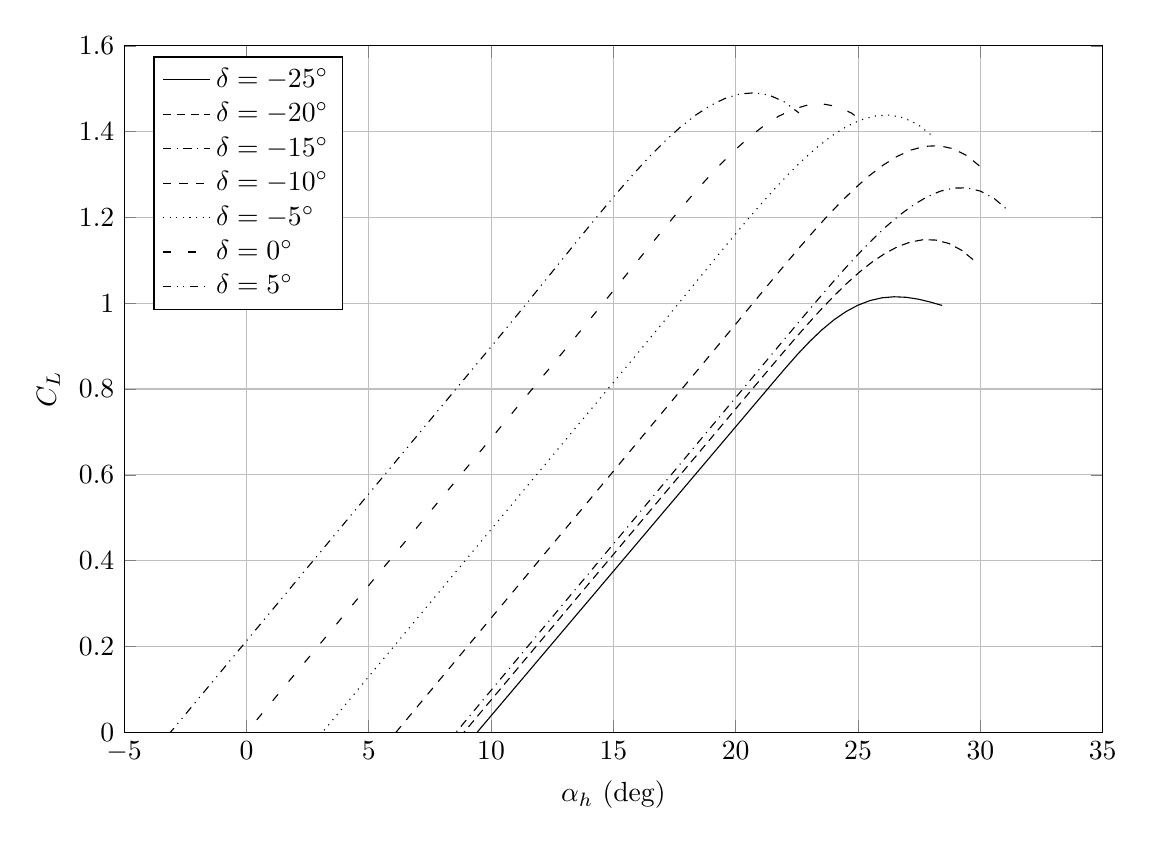
\begin{tikzpicture}

\begin{axis}[
width=14.01cm,
height=10.3cm,
scaled ticks=false, tick label style={/pgf/number format/fixed},
xmin=-5,
xmax=35,
xlabel={$\alpha_{h}$ (deg)},
xmajorgrids,
ymin=0,
ymax=1.6,
ylabel={$C_L$},
ymajorgrids,
legend style={at={(0.03,0.8)},anchor=west,draw=black,fill=white,legend cell align=left},
legend entries = {$\delta = -25^{\circ}$\\$\delta = -20^{\circ}$\\$\delta = -15^{\circ}$\\$\delta = -10^{\circ}$\\$\delta = -5^{\circ}$\\$\delta = 0^{\circ}$\\$\delta = 5^{\circ}$\\}
]

\addplot [
color=black,
solid
]
table[row sep=crcr]{
-0.5715576037630292	-0.6737465393512082\\
-0.07983053712342525	-0.6406165984058327\\
0.4118965295161787	-0.6074866574604574\\
0.9036235961557827	-0.5743567165150819\\
1.3953506627953867	-0.5412267755697066\\
1.8870777294349907	-0.5080968346243311\\
2.378804796074595	-0.4749668936789557\\
2.870531862714199	-0.44183695273358026\\
3.362258929353803	-0.4087070117882049\\
3.853985995993407	-0.37557707084282943\\
4.345713062633011	-0.3424471298974541\\
4.837440129272615	-0.30931718895207866\\
5.329167195912219	-0.27618724800670325\\
5.820894262551823	-0.24305730706132778\\
6.312621329191427	-0.20992736611595236\\
6.804348395831031	-0.17679742517057695\\
7.296075462470635	-0.14366748422520154\\
7.787802529110239	-0.11053754327982612\\
8.279529595749842	-0.07740760233445076\\
8.771256662389446	-0.04427766138907541\\
9.262983729029049	-0.011147720443700049\\
9.754710795668652	0.02198222050167531\\
10.246437862308255	0.05511216144705067\\
10.738164928947858	0.08824210239242603\\
11.229891995587462	0.12137204333780138\\
11.721619062227065	0.15450198428317674\\
12.213346128866668	0.1876319252285521\\
12.705073195506271	0.22076186617392746\\
13.196800262145874	0.2538918071193028\\
13.688527328785478	0.2870217480646782\\
14.18025439542508	0.32015168901005353\\
14.671981462064684	0.3532816299554289\\
15.163708528704287	0.38641157090080436\\
15.65543559534389	0.4195415118461797\\
16.147162661983494	0.4526714527915551\\
16.6388897286231	0.48580139373693043\\
17.130616795262704	0.518931334682306\\
17.62234386190231	0.5520612756276814\\
18.114070928541913	0.585191216573057\\
18.60579799518152	0.6183211575184323\\
19.097525061821123	0.6514510984638079\\
19.58925212846073	0.6845810394091832\\
20.080979195100333	0.7177109803545588\\
20.57270626173994	0.7508409212999344\\
21.064433328379543	0.7839708622453098\\
21.55616039501915	0.8171007671522332\\
22.047887461658753	0.8500018195479626\\
22.539614528298358	0.8817329808405177\\
23.031341594937963	0.9113465613120937\\
23.523068661577568	0.93806317995044\\
24.014795728217173	0.9612717644487603\\
24.506522794856778	0.980529551205997\\
24.998249861496383	0.9955620853264193\\
25.489976928135988	1.0062632206198785\\
25.981703994775593	1.0126951196020357\\
26.473431061415198	1.0150882534937082\\
26.965158128054803	1.0138414022215514\\
27.456885194694408	1.0095216544175187\\
27.948612261334013	1.0028644074194872\\
28.440339327973604	0.9947733672704899\\
};

\addplot [
color=black,
densely dashed
]
table[row sep=crcr]{
-1.108339630538266	-0.6787389411665551\\
-0.5851735423960166	-0.6432296214945632\\
-0.06200745425376719	-0.6077203018225713\\
0.4611586338884822	-0.5722109821505794\\
0.9843247220307316	-0.5367016624785875\\
1.507490810172981	-0.5011923428065956\\
2.03065689831523	-0.46568302313460375\\
2.5538229864574795	-0.43017370346261186\\
3.076989074599729	-0.39466438379061997\\
3.600155162741978	-0.3591550641186281\\
4.123321250884228	-0.32364574444663613\\
4.646487339026478	-0.2881364247746442\\
5.169653427168727	-0.2526271051026523\\
5.692819515310977	-0.21711778543066035\\
6.215985603453227	-0.18160846575866846\\
6.739151691595477	-0.1460991460866765\\
7.262317779737726	-0.11058982641468457\\
7.785483867879976	-0.07508050674269262\\
8.308649956022226	-0.03957118707070073\\
8.831816044164475	-0.0040618673987088405\\
9.354982132306723	0.03144745227328294\\
9.878148220448972	0.06695677194527483\\
10.401314308591221	0.10246609161726672\\
10.92448039673347	0.1379754112892586\\
11.447646484875719	0.1734847309612504\\
11.970812573017968	0.20899405063324228\\
12.493978661160217	0.24450337030523417\\
13.017144749302465	0.28001268997722606\\
13.540310837444714	0.31552200964921784\\
14.063476925586963	0.35103132932120973\\
14.586643013729212	0.3865406489932016\\
15.10980910187146	0.4220499686651934\\
15.63297519001371	0.4575592883371854\\
16.15614127815596	0.4930686080091774\\
16.67930736629821	0.5285779276811692\\
17.20247345444046	0.5640872473531612\\
17.725639542582712	0.5995965670251532\\
18.248805630724963	0.6351058866971452\\
18.771971718867213	0.6706152063691372\\
19.295137807009464	0.7061245260411292\\
19.818303895151715	0.7416338457131212\\
20.341469983293965	0.7771431653851132\\
20.864636071436216	0.8126524850571052\\
21.387802159578467	0.8481441377880596\\
21.910968247720717	0.883441250464994\\
22.434134335862968	0.9182573405597463\\
22.95730042400522	0.9522652150594286\\
23.48046651214747	0.9850975289851078\\
24.00363260028972	1.0163467853918178\\
24.52679868843197	1.0455653353685541\\
25.04996477657422	1.0722653780382814\\
25.57313086471647	1.0959189605579258\\
26.096296952858722	1.1159579781183737\\
26.619463041000973	1.1317741739444802\\
27.142629129143224	1.1427191392950746\\
27.665795217285474	1.148104313462925\\
28.188961305427725	1.1472009837747947\\
28.712127393569975	1.1392402855913755\\
29.235293481712226	1.1234132023073506\\
29.758459569854445	1.098870565351369\\
};

\addplot [
color=black,
dashdotted
]
table[row sep=crcr]{
-1.4332555184414915	-0.6825016951472419\\
-0.8816008886127704	-0.6448511731478492\\
-0.3299462587840494	-0.6072006511484567\\
0.22170837104467167	-0.569550129149064\\
0.7733630008733927	-0.5318996071496713\\
1.3250176307021138	-0.4942490851502787\\
1.8766722605308348	-0.4565985631508861\\
2.428326890359556	-0.4189480411514934\\
2.979981520188277	-0.3812975191521008\\
3.5316361500169977	-0.3436469971527082\\
4.0832907798457185	-0.3059964751533156\\
4.634945409674439	-0.26834595315392296\\
5.18660003950316	-0.23069543115453034\\
5.738254669331881	-0.19304490915513767\\
6.289909299160602	-0.15539438715574505\\
6.841563928989323	-0.11774386515635243\\
7.3932185588180435	-0.08009334315695982\\
7.944873188646764	-0.042442821157567256\\
8.496527818475485	-0.004792299158174584\\
9.048182448304207	0.03285822284121809\\
9.599837078132929	0.07050874484061076\\
10.15149170796165	0.10815926684000343\\
10.703146337790372	0.1458097888393961\\
11.254800967619094	0.18346031083878878\\
11.806455597447815	0.22111083283818156\\
12.358110227276537	0.25876135483757423\\
12.909764857105259	0.2964118768369669\\
13.46141948693398	0.3340623988363596\\
14.013074116762702	0.37171292083575225\\
14.564728746591424	0.4093634428351449\\
15.116383376420146	0.4470139648345377\\
15.668038006248867	0.48466448683393026\\
16.21969263607759	0.522315008833323\\
16.77134726590631	0.5599655308327156\\
17.323001895735032	0.5976160528321084\\
17.874656525563754	0.635266574831501\\
18.426311155392476	0.6729170968308937\\
18.977965785221198	0.7105676188302863\\
19.52962041504992	0.7482181408296791\\
20.08127504487864	0.7858686628290716\\
20.632929674707363	0.8235191848284644\\
21.184584304536084	0.8611730631123669\\
21.736238934364806	0.8988289810845442\\
22.287893564193528	0.9364287389612747\\
22.83954819402225	0.9738455819012755\\
23.39120282385097	1.0108841984132573\\
23.942857453679693	1.0472807203560022\\
24.494512083508415	1.0827027229382713\\
25.046166713337136	1.1167492247188546\\
25.597821343165858	1.1489506876065994\\
26.14947597299458	1.178769016860353\\
26.7011306028233	1.2055975610889744\\
27.252785232652023	1.2287611122513509\\
27.804439862480745	1.2475159056564165\\
28.356094492309467	1.2610496199631127\\
28.90774912213819	1.2684813771803958\\
29.45940375196691	1.2688617426672293\\
30.011058381795632	1.2611727251326483\\
30.562713011624353	1.2443277766356884\\
31.114367641453047	1.2171717925853853\\
};

\addplot [
color=black,
dashed
]
table[row sep=crcr]{
-3.886771815460465	-0.6848183705290662\\
-3.3119417088586225	-0.645452948835654\\
-2.73711160225678	-0.6060875271422417\\
-2.1622814956549377	-0.5667221054488294\\
-1.5874513890530952	-0.527356683755417\\
-1.0126212824512528	-0.4879912620620047\\
-0.4377911758494104	-0.4486258403685924\\
0.137038930752432	-0.40926041867518004\\
0.7118690373542744	-0.36989499698176775\\
1.2866991439561168	-0.3305295752883554\\
1.8615292505579593	-0.2911641535949431\\
2.4363593571598017	-0.2517987319015308\\
3.011189463761644	-0.21243331020811845\\
3.5860195703634865	-0.17306788851470614\\
4.160849676965329	-0.13370246682129383\\
4.735679783567171	-0.09433704512788149\\
5.310509890169014	-0.05497162343446921\\
5.885339996770856	-0.015606201741056869\\
6.460170103372699	0.02375921995235547\\
7.035000209974541	0.06312464164576775\\
7.609830316576383	0.10249006333918009\\
8.184660423178226	0.14185548503259238\\
8.759490529780068	0.18122090672600477\\
9.33432063638191	0.22058632841941705\\
9.909150742983753	0.25995175011282934\\
10.483980849585596	0.2993171718062416\\
11.058810956187438	0.338682593499654\\
11.63364106278928	0.3780480151930663\\
12.208471169391123	0.4174134368864786\\
12.783301275992965	0.456778858579891\\
13.358131382594808	0.49614428027330326\\
13.93296148919665	0.5355097019667155\\
14.507791595798492	0.5748751236601279\\
15.082621702400335	0.6142405453535401\\
15.657451809002177	0.6536059670469526\\
16.23228191560402	0.6929713887403649\\
16.807112022205864	0.7323368104337774\\
17.381942128807708	0.7717022321271897\\
17.956772235409552	0.8110676538206022\\
18.531602342011396	0.8504367333726464\\
19.10643244861324	0.8898682987287856\\
19.681262555215085	0.92942510855233\\
20.25609266181693	0.9691019087439834\\
20.830922768418773	1.0088232609146406\\
21.405752875020617	1.0484435423853888\\
21.98058298162246	1.0877469461875116\\
22.555413088224306	1.1264474810625025\\
23.13024319482615	1.164188971462032\\
23.705073301427994	1.2005450575479664\\
24.27990340802984	1.235019195192372\\
24.854733514631683	1.2670446559775073\\
25.429563621233527	1.2959845271958343\\
26.00439372783537	1.32113171184999\\
26.579223834437215	1.3417089286528245\\
27.15405394103906	1.3568687120273708\\
27.728884047640904	1.3656934121068751\\
28.303714154242748	1.3671951947347445\\
28.878544260844592	1.3603160414646212\\
29.453374367446436	1.3439277495603221\\
30.028204474048234	1.3168319319958393\\
};

\addplot [
color=black,
dotted
]
table[row sep=crcr]{
-6.894928847389513	-0.685608844934277\\
-6.302881888934857	-0.6450175818009821\\
-5.7108349304802	-0.6044263186676871\\
-5.118787972025543	-0.5638350555343923\\
-4.526741013570886	-0.5232437924010973\\
-3.9346940551162293	-0.48265252926780244\\
-3.3426470966615724	-0.4420612661345075\\
-2.7506001382069156	-0.4014700030012126\\
-2.158553179752259	-0.3608787398679177\\
-1.5665062212976022	-0.32028747673462277\\
-0.9744592628429456	-0.2796962136013279\\
-0.382412304388289	-0.23910495046803298\\
0.2096346540663676	-0.19851368733473806\\
0.8016816125210242	-0.15792242420144317\\
1.3937285709756808	-0.11733116106814827\\
1.9857755294303374	-0.07673989793485336\\
2.577822487884994	-0.03614863480155847\\
3.169869446339651	0.004442628331736448\\
3.7619164047943077	0.04503389146503137\\
4.3539633632489645	0.08562515459832629\\
4.946010321703621	0.1262164177316212\\
5.538057280158278	0.16680768086491612\\
6.130104238612935	0.20739894399821104\\
6.722151197067592	0.24799020713150596\\
7.314198155522249	0.28858147026480085\\
7.906245113976905	0.3291727333980957\\
8.498292072431562	0.3697639965313907\\
9.090339030886218	0.41035525966468556\\
9.682385989340874	0.4509465227979804\\
10.27443294779553	0.4915377859312753\\
10.866479906250186	0.5321290490645701\\
11.458526864704842	0.572720312197865\\
12.050573823159498	0.6133115753311598\\
12.642620781614154	0.6539028384644546\\
13.23466774006881	0.6944941015977495\\
13.826714698523466	0.7350853647310444\\
14.418761656978122	0.7756766278643392\\
15.010808615432778	0.8162678909976342\\
15.602855573887433	0.8568676655740002\\
16.19490253234209	0.8975683361758855\\
16.786949490796747	0.9384690097882626\\
17.378996449251403	0.9796019727605345\\
17.97104340770606	1.020931599494713\\
18.563090366160715	1.0623543524454413\\
19.15513732461537	1.1036987821199706\\
19.747184283070027	1.1447255270781747\\
20.339231241524683	1.1851273139325476\\
20.93127819997934	1.2245289573482023\\
21.523325158433995	1.2624873600428654\\
22.11537211688865	1.2984915127868786\\
22.707419075343307	1.33196249440322\\
23.299466033797962	1.3622534717674672\\
23.89151299225262	1.3886496998078308\\
24.483559950707274	1.4103685215051134\\
25.07560690916193	1.426559367892779\\
25.667653867616586	1.436303758056877\\
26.259700826071242	1.4386152991360786\\
26.851747784525898	1.4324396863216902\\
27.443794742980554	1.416654702857619\\
28.035841701435228	1.3900702200404038\\
};

\addplot [
color=black,
loosely dashed
]
table[row sep=crcr]{
-10.0	-0.6848548567243371\\
-9.401146502112754	-0.6438420840748933\\
-8.802293004225508	-0.6028293114254495\\
-8.203439506338261	-0.5618165387760057\\
-7.604586008451015	-0.5208037661265619\\
-7.005732510563769	-0.479790993477118\\
-6.406879012676523	-0.4387782208276742\\
-5.808025514789277	-0.3977654481782304\\
-5.209172016902031	-0.3567526755287866\\
-4.610318519014784	-0.3157399028793428\\
-4.011465021127538	-0.274727130229899\\
-3.412611523240292	-0.23371435758045517\\
-2.813758025353046	-0.1927015849310114\\
-2.2149045274657997	-0.15168881228156758\\
-1.6160510295785535	-0.11067603963212376\\
-1.0171975316913073	-0.06966326698267995\\
-0.41834403380406104	-0.028650494333236146\\
0.18050946408318524	0.01236227831620767\\
0.7793629619704315	0.05337505096565148\\
1.3782164598576778	0.09438782361509529\\
1.977069957744924	0.1354005962645391\\
2.57592345563217	0.1764133689139829\\
3.1747769535194164	0.2174261415634267\\
3.7736304514066625	0.2584389142128705\\
4.372483949293909	0.2994516868623144\\
4.971337447181155	0.3404644595117582\\
5.5701909450684015	0.381477232161202\\
6.169044442955648	0.42249000481064575\\
6.767897940842894	0.46350277746008955\\
7.36675143873014	0.5045155501095334\\
7.965604936617386	0.5455283227589772\\
8.564458434504633	0.586541095408421\\
9.16331193239188	0.6275538680578648\\
9.762165430279126	0.6685666407073086\\
10.361018928166372	0.7095794133567525\\
10.959872426053618	0.7505921860061963\\
11.558725923940864	0.7916049586556401\\
12.15757942182811	0.8326177593838535\\
12.756432919715357	0.8736684534047081\\
13.355286417602603	0.914883089342833\\
13.954139915489849	0.9563464753724176\\
14.552993413377095	0.9980768043617123\\
15.151846911264341	1.0400256538730235\\
15.750700409151587	1.0820779861627232\\
16.349553907038835	1.124052148181237\\
16.948407404926083	1.1656998715730478\\
17.54726090281333	1.206706272676705\\
18.14611440070058	1.246689852524811\\
18.744967898587827	1.28520249684403\\
19.343821396475075	1.3217294760550857\\
19.942674894362323	1.3556894452727593\\
20.54152839224957	1.3864344443058914\\
21.14038189013682	1.4132498976573837\\
21.739235388024067	1.4353546145241947\\
22.338088885911315	1.4519007887973399\\
22.936942383798563	1.4619739990619032\\
23.53579588168581	1.4645932085970135\\
24.13464937957306	1.4587107653758713\\
24.733502877460307	1.4432124020657364\\
25.33235637534753	1.416917236027918\\
};

\addplot [
color=black,
dashdotdotted
]
table[row sep=crcr]{
-13.105071152610487	-0.685608844934277\\
-12.500208446441835	-0.644138922802266\\
-11.895345740273184	-0.602669000670255\\
-11.290483034104533	-0.561199078538244\\
-10.685620327935881	-0.519729156406233\\
-10.08075762176723	-0.478259234274222\\
-9.475894915598579	-0.43678931214221095\\
-8.871032209429927	-0.3953193900102\\
-8.266169503261276	-0.35384946787818894\\
-7.661306797092624	-0.3123795457461779\\
-7.056444090923971	-0.27090962361416693\\
-6.451581384755319	-0.22943970148215584\\
-5.846718678586667	-0.18796977935014478\\
-5.241855972418015	-0.14649985721813366\\
-4.6369932662493625	-0.1050299350861226\\
-4.03213056008071	-0.06356001295411154\\
-3.427267853912058	-0.022090090822100478\\
-2.822405147743406	0.019379831309910583\\
-2.2175424415747536	0.060849753441921645\\
-1.6126797354061013	0.1023196755739327\\
-1.007817029237449	0.1437895977059438\\
-0.40295432306879697	0.18525951983795483\\
0.20190838309985515	0.2267294419699659\\
0.8067710892685073	0.268199364101977\\
1.4116337954371594	0.30966928623398804\\
2.0164965016058116	0.3511392083659991\\
2.621359207774464	0.39260913049801016\\
3.226221913943116	0.4340790526300212\\
3.8310846201117683	0.4755489747620323\\
4.43594732628042	0.5170188968940433\\
5.040810032449072	0.5584888190260544\\
5.645672738617725	0.5999587411580655\\
6.250535444786377	0.6414286632900765\\
6.855398150955029	0.6828985854220876\\
7.460260857123681	0.7243685075540987\\
8.065123563292333	0.7658384296861097\\
8.669986269460985	0.8073083518181208\\
9.274848975629636	0.8487814521133863\\
9.879711681798288	0.8903400133585712\\
10.484574387966939	0.9321155138287641\\
11.08943709413559	0.9741792816160535\\
11.694299800304242	1.0165370996307066\\
12.299162506472893	1.0591292056011725\\
12.904025212641544	1.1018302920740777\\
13.508887918810196	1.1444495064142293\\
14.113750624978847	1.1867304508046148\\
14.718613331147498	1.2283511822464006\\
15.32347603731615	1.2689242125589324\\
15.928338743484801	1.3079965083797362\\
16.533201449653454	1.3450494911645188\\
17.138064155822107	1.3794990371871632\\
17.74292686199076	1.4106954775397353\\
18.347789568159413	1.4379235981324787\\
18.952652274328067	1.460402639693819\\
19.55751498049672	1.4772862977703602\\
20.162377686665373	1.487662722726887\\
20.767240392834026	1.4905545197463579\\
21.37210309900268	1.4849187488299203\\
21.976965805171332	1.4696469247968933\\
22.581828511339992	1.4435650172847834\\
};
\end{axis}
\end{tikzpicture}%

\caption{ATR 72 . Mach 0.45. CL vs $\alpha_h$ for the horizontal tail with elevator deflections.}
\label{fig:stallATR}
\end{figure}
\noindent\\
\begin{figure}[H]
\centering
%Comparison of CD estimation
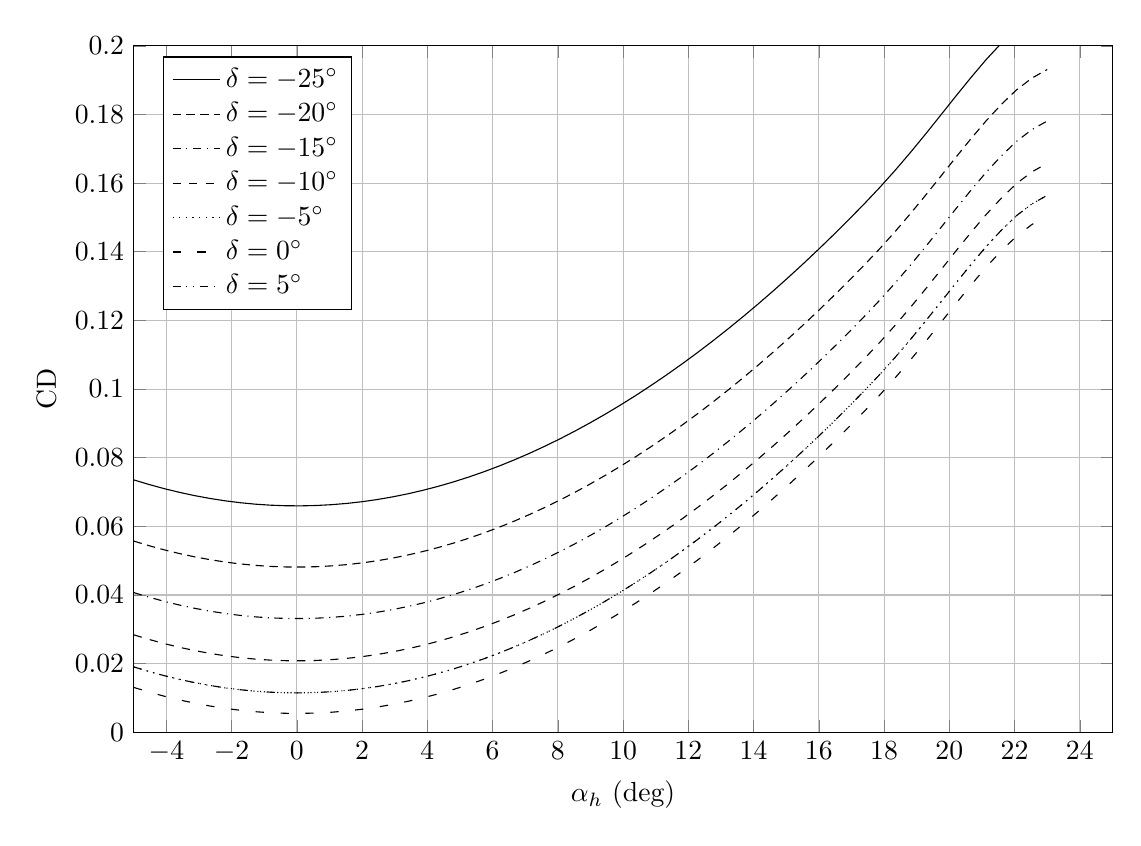
\begin{tikzpicture}

\begin{axis}[
width=14.01cm,
height=10.3cm,
scaled ticks=false, tick label style={/pgf/number format/fixed},
xmin=-5,
xmax=25,
xlabel={$\alpha_{h}$ (deg)},
xmajorgrids,
ymin=0,
ymax=0.2,
ylabel={CD},
ymajorgrids,
legend style={at={(0.03,0.8)},anchor=west,draw=black,fill=white,legend cell align=left},
legend entries = {$\delta = -25^{\circ}$\\$\delta = -20^{\circ}$\\$\delta = -15^{\circ}$\\$\delta = -10^{\circ}$\\$\delta = -5^{\circ}$\\$\delta = 0^{\circ}$\\$\delta = 5^{\circ}$\\}
]

\addplot [
color=black,
solid
]
table[row sep=crcr]{
-4.999999999999999	0.07353663868712164\\
-4.533333333333332	0.07219962776162059\\
-4.0666666666666655	0.07098449154538652\\
-3.5999999999999988	0.06990558261316618\\
-3.133333333333332	0.06895081086082233\\
-2.666666666666665	0.0681324095185158\\
-2.1999999999999984	0.0674402146216418\\
-1.7333333333333318	0.0668843071264542\\
-1.2666666666666653	0.06645641639488947\\
-0.7999999999999987	0.06616444073708463\\
-0.33333333333333215	0.06600197733773967\\
0.13333333333333441	0.06597472168561698\\
0.600000000000001	0.06607812327413246\\
1.0666666666666675	0.06631566458205995\\
1.533333333333334	0.06668464647230998\\
2.000000000000001	0.06718634560652714\\
2.4666666666666677	0.06781992620292263\\
2.9333333333333345	0.06858447762332077\\
3.4000000000000012	0.06948105153887923\\
3.866666666666668	0.07050657656388111\\
4.333333333333335	0.07166402286459263\\
4.800000000000002	0.07294819367153564\\
5.266666666666668	0.07436401185104223\\
5.733333333333335	0.07590418759784258\\
6.200000000000002	0.07757562889818638\\
6.666666666666669	0.07936898208903245\\
7.1333333333333355	0.0812931663735236\\
7.600000000000002	0.08333679076643682\\
8.066666666666668	0.08551080807229326\\
8.533333333333335	0.08780180614612809\\
9.000000000000002	0.09022278575603968\\
9.466666666666669	0.09275883366437031\\
9.933333333333335	0.09542348444196036\\
10.400000000000002	0.09820236141277502\\
10.866666666666669	0.10110750648706285\\
11.333333333333336	0.10412660551664682\\
11.800000000000002	0.10726970120212925\\
12.26666666666667	0.11052654188247404\\
12.733333333333336	0.11390517001872644\\
13.200000000000003	0.11739739464116883\\
13.66666666666667	0.1210092556034979\\
14.133333333333336	0.124734619852793\\
14.600000000000003	0.1285775221855835\\
15.06666666666667	0.132533884036978\\
15.533333333333337	0.1366057298771524\\
16.000000000000004	0.1407910329234757\\
16.46666666666667	0.1450898067423312\\
16.933333333333334	0.14950207284753642\\
17.4	0.15403016561779484\\
17.866666666666664	0.1587196079474598\\
18.33333333333333	0.16364857989488765\\
18.799999999999994	0.16883657828918497\\
19.26666666666666	0.1742225574742876\\
19.733333333333324	0.17975779417442378\\
20.19999999999999	0.18532634700062064\\
20.666666666666654	0.1907881659349079\\
21.13333333333332	0.19602606195777136\\
21.599999999999984	0.20080163789459077\\
22.06666666666665	0.20505236864682802\\
22.533333333333314	0.20841749324832917\\
22.999999999999993	0.21091502753197286\\
};

\addplot [
color=black,
densely dashed
]
table[row sep=crcr]{
-4.999999999999999	0.055705722344289645\\
-4.533333333333332	0.054368711418788594\\
-4.0666666666666655	0.05315357520255452\\
-3.5999999999999988	0.05207466627033419\\
-3.133333333333332	0.05111989451799033\\
-2.666666666666665	0.050301493175683804\\
-2.1999999999999984	0.049609298278809805\\
-1.7333333333333318	0.049053390783622204\\
-1.2666666666666653	0.048625500052057485\\
-0.7999999999999987	0.04833352439425264\\
-0.33333333333333215	0.04817106099490767\\
0.13333333333333441	0.04814380534278499\\
0.600000000000001	0.04824720693130047\\
1.0666666666666675	0.04848474823922796\\
1.533333333333334	0.048853730129477996\\
2.000000000000001	0.04935542926369514\\
2.4666666666666677	0.04998900986009064\\
2.9333333333333345	0.05075356128048878\\
3.4000000000000012	0.05165013519604725\\
3.866666666666668	0.052675660221049116\\
4.333333333333335	0.05383310652176064\\
4.800000000000002	0.05511727732870365\\
5.266666666666668	0.056533095508210236\\
5.733333333333335	0.05807327125501059\\
6.200000000000002	0.05974471255535439\\
6.666666666666669	0.06153806574620045\\
7.1333333333333355	0.06346225003069161\\
7.600000000000002	0.06550587442360484\\
8.066666666666668	0.06767989172946128\\
8.533333333333335	0.0699708898032961\\
9.000000000000002	0.07239186941320769\\
9.466666666666669	0.0749279173215383\\
9.933333333333335	0.07759256809912836\\
10.400000000000002	0.08037144506994304\\
10.866666666666669	0.08327659014423085\\
11.333333333333336	0.08629568917381483\\
11.800000000000002	0.08943878485929727\\
12.26666666666667	0.09269562553964206\\
12.733333333333336	0.09607425367589445\\
13.200000000000003	0.09956647829833684\\
13.66666666666667	0.10317833926066591\\
14.133333333333336	0.10690370350996099\\
14.600000000000003	0.11074660584275149\\
15.06666666666667	0.114702967694146\\
15.533333333333337	0.11877481353432039\\
16.000000000000004	0.1229601165806437\\
16.46666666666667	0.12725889039949922\\
16.933333333333334	0.13167115650470443\\
17.4	0.13619924927496285\\
17.866666666666664	0.1408886916046278\\
18.33333333333333	0.14581766355205567\\
18.799999999999994	0.15100566194635295\\
19.26666666666666	0.1563916411314556\\
19.733333333333324	0.1619268778315918\\
20.19999999999999	0.16749543065778866\\
20.666666666666654	0.17295724959207592\\
21.13333333333332	0.17819514561493938\\
21.599999999999984	0.18297072155175875\\
22.06666666666665	0.187221452303996\\
22.533333333333314	0.19058657690549718\\
22.999999999999993	0.19308411118914087\\
};

\addplot [
color=black,
dashdotted
]
table[row sep=crcr]{
-4.999999999999999	0.0407043777572975\\
-4.533333333333332	0.03936736683179645\\
-4.0666666666666655	0.03815223061556238\\
-3.5999999999999988	0.03707332168334205\\
-3.133333333333332	0.03611854993099819\\
-2.666666666666665	0.03530014858869167\\
-2.1999999999999984	0.03460795369181767\\
-1.7333333333333318	0.03405204619663006\\
-1.2666666666666653	0.03362415546506534\\
-0.7999999999999987	0.0333321798072605\\
-0.33333333333333215	0.03316971640791553\\
0.13333333333333441	0.03314246075579285\\
0.600000000000001	0.033245862344308326\\
1.0666666666666675	0.033483403652235816\\
1.533333333333334	0.033852385542485854\\
2.000000000000001	0.034354084676703\\
2.4666666666666677	0.034987665273098496\\
2.9333333333333345	0.03575221669349664\\
3.4000000000000012	0.0366487906090551\\
3.866666666666668	0.037674315634056973\\
4.333333333333335	0.0388317619347685\\
4.800000000000002	0.040115932741711505\\
5.266666666666668	0.041531750921218094\\
5.733333333333335	0.04307192666801845\\
6.200000000000002	0.044743367968362244\\
6.666666666666669	0.04653672115920831\\
7.1333333333333355	0.04846090544369947\\
7.600000000000002	0.05050452983661269\\
8.066666666666668	0.052678547142469126\\
8.533333333333335	0.05496954521630396\\
9.000000000000002	0.057390524826215546\\
9.466666666666669	0.05992657273454617\\
9.933333333333335	0.06259122351213622\\
10.400000000000002	0.06537010048295089\\
10.866666666666669	0.06827524555723871\\
11.333333333333336	0.07129434458682268\\
11.800000000000002	0.07443744027230512\\
12.26666666666667	0.07769428095264991\\
12.733333333333336	0.0810729090889023\\
13.200000000000003	0.08456513371134469\\
13.66666666666667	0.08817699467367376\\
14.133333333333336	0.09190235892296886\\
14.600000000000003	0.09574526125575936\\
15.06666666666667	0.09970162310715386\\
15.533333333333337	0.10377346894732825\\
16.000000000000004	0.10795877199365156\\
16.46666666666667	0.11225754581250708\\
16.933333333333334	0.11666981191771228\\
17.4	0.1211979046879707\\
17.866666666666664	0.12588734701763565\\
18.33333333333333	0.13081631896506352\\
18.799999999999994	0.13600431735936083\\
19.26666666666666	0.14139029654446347\\
19.733333333333324	0.14692553324459964\\
20.19999999999999	0.1524940860707965\\
20.666666666666654	0.15795590500508377\\
21.13333333333332	0.16319380102794723\\
21.599999999999984	0.16796937696476663\\
22.06666666666665	0.17222010771700388\\
22.533333333333314	0.17558523231850504\\
22.999999999999993	0.17808276660214872\\
};

\addplot [
color=black,
dashed
]
table[row sep=crcr]{
-4.999999999999999	0.02839393452771092\\
-4.533333333333332	0.02705692360220987\\
-4.0666666666666655	0.025841787385975798\\
-3.5999999999999988	0.024762878453755466\\
-3.133333333333332	0.023808106701411605\\
-2.666666666666665	0.02298970535910508\\
-2.1999999999999984	0.022297510462231083\\
-1.7333333333333318	0.02174160296704348\\
-1.2666666666666653	0.02131371223547876\\
-0.7999999999999987	0.021021736577673915\\
-0.33333333333333215	0.020859273178328946\\
0.13333333333333441	0.020832017526206267\\
0.600000000000001	0.020935419114721743\\
1.0666666666666675	0.02117296042264923\\
1.533333333333334	0.02154194231289927\\
2.000000000000001	0.022043641447116416\\
2.4666666666666677	0.02267722204351191\\
2.9333333333333345	0.023441773463910055\\
3.4000000000000012	0.02433834737946852\\
3.866666666666668	0.02536387240447039\\
4.333333333333335	0.026521318705181915\\
4.800000000000002	0.02780548951212492\\
5.266666666666668	0.02922130769163151\\
5.733333333333335	0.030761483438431866\\
6.200000000000002	0.03243292473877567\\
6.666666666666669	0.034226277929621726\\
7.1333333333333355	0.03615046221411289\\
7.600000000000002	0.038194086607026105\\
8.066666666666668	0.04036810391288255\\
8.533333333333335	0.04265910198671738\\
9.000000000000002	0.04508008159662896\\
9.466666666666669	0.04761612950495959\\
9.933333333333335	0.050280780282549634\\
10.400000000000002	0.053059657253364305\\
10.866666666666669	0.05596480232765212\\
11.333333333333336	0.05898390135723611\\
11.800000000000002	0.06212699704271853\\
12.26666666666667	0.06538383772306333\\
12.733333333333336	0.06876246585931572\\
13.200000000000003	0.07225469048175812\\
13.66666666666667	0.07586655144408719\\
14.133333333333336	0.07959191569338227\\
14.600000000000003	0.08343481802617277\\
15.06666666666667	0.08739117987756727\\
15.533333333333337	0.09146302571774166\\
16.000000000000004	0.09564832876406497\\
16.46666666666667	0.0999471025829205\\
16.933333333333334	0.1043593686881257\\
17.4	0.10888746145838411\\
17.866666666666664	0.11357690378804908\\
18.33333333333333	0.11850587573547693\\
18.799999999999994	0.12369387412977424\\
19.26666666666666	0.12907985331487687\\
19.733333333333324	0.13461509001501307\\
20.19999999999999	0.14018364284120993\\
20.666666666666654	0.1456454617754972\\
21.13333333333332	0.15088335779836065\\
21.599999999999984	0.15565893373518003\\
22.06666666666665	0.15990966448741728\\
22.533333333333314	0.16327478908891846\\
22.999999999999993	0.16577232337256215\\
};

\addplot [
color=black,
dotted
]
table[row sep=crcr]{
-4.999999999999999	0.019052215956305886\\
-4.533333333333332	0.017715205030804836\\
-4.0666666666666655	0.016500068814570765\\
-3.5999999999999988	0.015421159882350433\\
-3.133333333333332	0.014466388130006573\\
-2.666666666666665	0.01364798678770005\\
-2.1999999999999984	0.012955791890826051\\
-1.7333333333333318	0.012399884395638446\\
-1.2666666666666653	0.011971993664073727\\
-0.7999999999999987	0.011680018006268885\\
-0.33333333333333215	0.011517554606923917\\
0.13333333333333441	0.011490298954801234\\
0.600000000000001	0.01159370054331671\\
1.0666666666666675	0.0118312418512442\\
1.533333333333334	0.012200223741494237\\
2.000000000000001	0.012701922875711386\\
2.4666666666666677	0.01333550347210688\\
2.9333333333333345	0.014100054892505024\\
3.4000000000000012	0.014996628808063487\\
3.866666666666668	0.016022153833065357\\
4.333333333333335	0.01717960013377688\\
4.800000000000002	0.018463770940719892\\
5.266666666666668	0.019879589120226478\\
5.733333333333335	0.021419764867026833\\
6.200000000000002	0.023091206167370634\\
6.666666666666669	0.024884559358216693\\
7.1333333333333355	0.026808743642707855\\
7.600000000000002	0.028852368035621072\\
8.066666666666668	0.031026385341477516\\
8.533333333333335	0.033317383415312346\\
9.000000000000002	0.03573836302522393\\
9.466666666666669	0.038274410933554555\\
9.933333333333335	0.0409390617111446\\
10.400000000000002	0.04371793868195927\\
10.866666666666669	0.04662308375624709\\
11.333333333333336	0.049642182785831074\\
11.800000000000002	0.0527852784713135\\
12.26666666666667	0.0560421191516583\\
12.733333333333336	0.05942074728791069\\
13.200000000000003	0.06291297191035308\\
13.66666666666667	0.06652483287268215\\
14.133333333333336	0.07025019712197723\\
14.600000000000003	0.07409309945476773\\
15.06666666666667	0.07804946130616223\\
15.533333333333337	0.08212130714633663\\
16.000000000000004	0.08630661019265994\\
16.46666666666667	0.09060538401151547\\
16.933333333333334	0.09501765011672067\\
17.4	0.09954574288697908\\
17.866666666666664	0.10423518521664404\\
18.33333333333333	0.10916415716407189\\
18.799999999999994	0.11435215555836921\\
19.26666666666666	0.11973813474347185\\
19.733333333333324	0.12527337144360803\\
20.19999999999999	0.1308419242698049\\
20.666666666666654	0.13630374320409216\\
21.13333333333332	0.14154163922695562\\
21.599999999999984	0.14631721516377502\\
22.06666666666665	0.15056794591601227\\
22.533333333333314	0.15393307051751343\\
22.999999999999993	0.1564306048011571\\
};

\addplot [
color=black,
loosely dashed
]
table[row sep=crcr]{
-4.999999999999999	0.01307062850857717\\
-4.533333333333332	0.011733617583076119\\
-4.0666666666666655	0.01051848136684205\\
-3.5999999999999988	0.009439572434621716\\
-3.133333333333332	0.008484800682277856\\
-2.666666666666665	0.007666399339971333\\
-2.1999999999999984	0.006974204443097334\\
-1.7333333333333318	0.006418296947909729\\
-1.2666666666666653	0.00599040621634501\\
-0.7999999999999987	0.005698430558540168\\
-0.33333333333333215	0.0055359671591952\\
0.13333333333333441	0.005508711507072517\\
0.600000000000001	0.005612113095587993\\
1.0666666666666675	0.005849654403515482\\
1.533333333333334	0.006218636293765521\\
2.000000000000001	0.006720335427982669\\
2.4666666666666677	0.007353916024378162\\
2.9333333333333345	0.008118467444776307\\
3.4000000000000012	0.00901504136033477\\
3.866666666666668	0.010040566385336642\\
4.333333333333335	0.011198012686048165\\
4.800000000000002	0.012482183492991175\\
5.266666666666668	0.01389800167249776\\
5.733333333333335	0.015438177419298116\\
6.200000000000002	0.017109618719641916\\
6.666666666666669	0.018902971910487978\\
7.1333333333333355	0.02082715619497914\\
7.600000000000002	0.022870780587892357\\
8.066666666666668	0.025044797893748798\\
8.533333333333335	0.02733579596758363\\
9.000000000000002	0.029756775577495214\\
9.466666666666669	0.03229282348582584\\
9.933333333333335	0.03495747426341589\\
10.400000000000002	0.03773635123423056\\
10.866666666666669	0.04064149630851838\\
11.333333333333336	0.04366059533810236\\
11.800000000000002	0.04680369102358479\\
12.26666666666667	0.05006053170392959\\
12.733333333333336	0.05343915984018198\\
13.200000000000003	0.05693138446262437\\
13.66666666666667	0.06054324542495344\\
14.133333333333336	0.06426860967424852\\
14.600000000000003	0.06811151200703902\\
15.06666666666667	0.07206787385843352\\
15.533333333333337	0.07613971969860792\\
16.000000000000004	0.08032502274493122\\
16.46666666666667	0.08462379656378675\\
16.933333333333334	0.08903606266899196\\
17.4	0.09356415543925037\\
17.866666666666664	0.09825359776891533\\
18.33333333333333	0.10318256971634318\\
18.799999999999994	0.1083705681106405\\
19.26666666666666	0.11375654729574314\\
19.733333333333324	0.11929178399587932\\
20.19999999999999	0.12486033682207619\\
20.666666666666654	0.13032215575636344\\
21.13333333333332	0.1355600517792269\\
21.599999999999984	0.1403356277160463\\
22.06666666666665	0.14458635846828355\\
22.533333333333314	0.1479514830697847\\
22.999999999999993	0.1504490173534284\\
};

\addplot [
color=black,
dashdotdotted
]
table[row sep=crcr]{
-4.999999999999999	0.019052215956305886\\
-4.533333333333332	0.017715205030804836\\
-4.0666666666666655	0.016500068814570765\\
-3.5999999999999988	0.015421159882350433\\
-3.133333333333332	0.014466388130006573\\
-2.666666666666665	0.01364798678770005\\
-2.1999999999999984	0.012955791890826051\\
-1.7333333333333318	0.012399884395638446\\
-1.2666666666666653	0.011971993664073727\\
-0.7999999999999987	0.011680018006268885\\
-0.33333333333333215	0.011517554606923917\\
0.13333333333333441	0.011490298954801234\\
0.600000000000001	0.01159370054331671\\
1.0666666666666675	0.0118312418512442\\
1.533333333333334	0.012200223741494237\\
2.000000000000001	0.012701922875711386\\
2.4666666666666677	0.01333550347210688\\
2.9333333333333345	0.014100054892505024\\
3.4000000000000012	0.014996628808063487\\
3.866666666666668	0.016022153833065357\\
4.333333333333335	0.01717960013377688\\
4.800000000000002	0.018463770940719892\\
5.266666666666668	0.019879589120226478\\
5.733333333333335	0.021419764867026833\\
6.200000000000002	0.023091206167370634\\
6.666666666666669	0.024884559358216693\\
7.1333333333333355	0.026808743642707855\\
7.600000000000002	0.028852368035621072\\
8.066666666666668	0.031026385341477516\\
8.533333333333335	0.033317383415312346\\
9.000000000000002	0.03573836302522393\\
9.466666666666669	0.038274410933554555\\
9.933333333333335	0.0409390617111446\\
10.400000000000002	0.04371793868195927\\
10.866666666666669	0.04662308375624709\\
11.333333333333336	0.049642182785831074\\
11.800000000000002	0.0527852784713135\\
12.26666666666667	0.0560421191516583\\
12.733333333333336	0.05942074728791069\\
13.200000000000003	0.06291297191035308\\
13.66666666666667	0.06652483287268215\\
14.133333333333336	0.07025019712197723\\
14.600000000000003	0.07409309945476773\\
15.06666666666667	0.07804946130616223\\
15.533333333333337	0.08212130714633663\\
16.000000000000004	0.08630661019265994\\
16.46666666666667	0.09060538401151547\\
16.933333333333334	0.09501765011672067\\
17.4	0.09954574288697908\\
17.866666666666664	0.10423518521664404\\
18.33333333333333	0.10916415716407189\\
18.799999999999994	0.11435215555836921\\
19.26666666666666	0.11973813474347185\\
19.733333333333324	0.12527337144360803\\
20.19999999999999	0.1308419242698049\\
20.666666666666654	0.13630374320409216\\
21.13333333333332	0.14154163922695562\\
21.599999999999984	0.14631721516377502\\
22.06666666666665	0.15056794591601227\\
22.533333333333314	0.15393307051751343\\
22.999999999999993	0.1564306048011571\\
};
\end{axis}
\end{tikzpicture}%

\caption{ATR 72 . Mach 0.45. CD vs $\alpha_h$ for the horizontal tail with elevator deflections.}
\label{fig:stallATR}
\end{figure}
\begin{figure}[H]
\centering
%Comparison of CD estimation
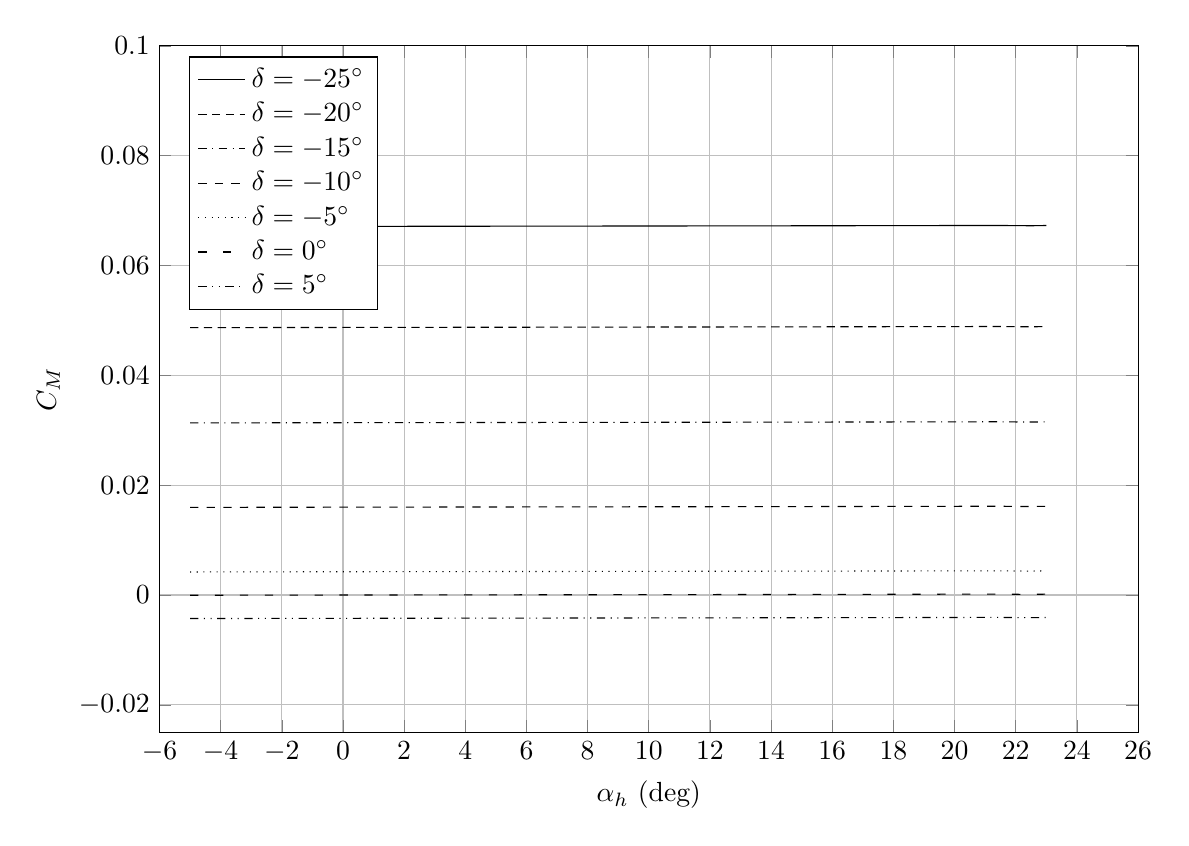
\begin{tikzpicture}

\begin{axis}[
width=14.01cm,
height=10.3cm,
scaled ticks=false, tick label style={/pgf/number format/fixed},
xmin=-6,
xmax=26,
xlabel={$\alpha_{h}$ (deg)},
xmajorgrids,
ymin=-0.025,
ymax=0.1,
ylabel={$C_M$},
ymajorgrids,
legend style={at={(0.03,0.8)},anchor=west,draw=black,fill=white,legend cell align=left},
legend entries = {$\delta = -25^{\circ}$\\$\delta = -20^{\circ}$\\$\delta = -15^{\circ}$\\$\delta = -10^{\circ}$\\$\delta = -5^{\circ}$\\$\delta = 0^{\circ}$\\$\delta = 5^{\circ}$\\}
]

\addplot [
color=black,
solid
]
table[row sep=crcr]{
-4.999999999999999	0.06707761761287616\\
-4.533333333333332	0.06708197777674768\\
-4.0666666666666655	0.0670863379406192\\
-3.5999999999999988	0.06709069810449068\\
-3.133333333333332	0.06709505826836216\\
-2.666666666666665	0.06709941843223366\\
-2.1999999999999984	0.06710294416440286\\
-1.7333333333333318	0.06710638030860762\\
-1.2666666666666653	0.06710981012497004\\
-0.7999999999999987	0.06711323358727801\\
-0.33333333333333215	0.06711665067008495\\
0.13333333333333441	0.06712006114266882\\
0.600000000000001	0.06712346509267438\\
1.0666666666666675	0.06712686258946611\\
1.533333333333334	0.06713025361104874\\
2.000000000000001	0.06713363813631411\\
2.4666666666666677	0.06713701614506307\\
2.9333333333333345	0.0671403875245665\\
3.4000000000000012	0.06714375213781894\\
3.866666666666668	0.0671471101779963\\
4.333333333333335	0.06715046162891926\\
4.800000000000002	0.06715380647542421\\
5.266666666666668	0.06715714470338141\\
5.733333333333335	0.06716047629971295\\
6.200000000000002	0.06716380096678011\\
6.666666666666669	0.06716711895485232\\
7.1333333333333355	0.06717043027775246\\
7.600000000000002	0.06717373492696856\\
8.066666666666668	0.06717703153487732\\
8.533333333333335	0.06718030333669306\\
9.000000000000002	0.0671835556179337\\
9.466666666666669	0.06718680127132619\\
9.933333333333335	0.06719005044076054\\
10.400000000000002	0.06719331312024754\\
10.866666666666669	0.06719659946488654\\
11.333333333333336	0.06719991979519624\\
11.800000000000002	0.06720328510634364\\
12.26666666666667	0.06720670893511627\\
12.733333333333336	0.0672102003283196\\
13.200000000000003	0.06721377039005462\\
13.66666666666667	0.06721743044332158\\
14.133333333333336	0.06722119204628021\\
14.600000000000003	0.06722506701050221\\
15.06666666666667	0.06722907290583545\\
15.533333333333337	0.06723321971069772\\
16.000000000000004	0.06723751884970035\\
16.46666666666667	0.06724198344683766\\
16.933333333333334	0.06724662700996376\\
17.4	0.06725143098574066\\
17.866666666666664	0.06725579114961198\\
18.33333333333333	0.06726015131348358\\
18.799999999999994	0.0672645114773549\\
19.26666666666666	0.0672688716412265\\
19.733333333333324	0.06727323180509798\\
20.19999999999999	0.06727759196896957\\
20.666666666666654	0.06728195213284094\\
21.13333333333332	0.0672863122967124\\
21.599999999999984	0.06727989366275047\\
22.06666666666665	0.0672525995326312\\
22.533333333333314	0.0672390003547999\\
22.999999999999993	0.06728014994169734\\
};

\addplot [
color=black,
densely dashed
]
table[row sep=crcr]{
-4.999999999999999	0.0486772769525898\\
-4.533333333333332	0.04868163711646131\\
-4.0666666666666655	0.048685997280332835\\
-3.5999999999999988	0.04869035744420433\\
-3.133333333333332	0.0486947176080758\\
-2.666666666666665	0.0486990777719473\\
-2.1999999999999984	0.04870260350411651\\
-1.7333333333333318	0.04870603964832125\\
-1.2666666666666653	0.04870946946468368\\
-0.7999999999999987	0.04871289292699165\\
-0.33333333333333215	0.04871631000979859\\
0.13333333333333441	0.04871972048238245\\
0.600000000000001	0.048723124432388014\\
1.0666666666666675	0.04872652192917975\\
1.533333333333334	0.048729912950762386\\
2.000000000000001	0.048733297476027754\\
2.4666666666666677	0.0487366754847767\\
2.9333333333333345	0.048740046864280136\\
3.4000000000000012	0.04874341147753257\\
3.866666666666668	0.048746769517709926\\
4.333333333333335	0.0487501209686329\\
4.800000000000002	0.04875346581513785\\
5.266666666666668	0.048756804043095056\\
5.733333333333335	0.04876013563942658\\
6.200000000000002	0.04876346030649374\\
6.666666666666669	0.048766778294565966\\
7.1333333333333355	0.04877008961746611\\
7.600000000000002	0.04877339426668219\\
8.066666666666668	0.04877669087459097\\
8.533333333333335	0.048779962676406705\\
9.000000000000002	0.048783214957647335\\
9.466666666666669	0.04878646061103983\\
9.933333333333335	0.04878970978047417\\
10.400000000000002	0.04879297245996118\\
10.866666666666669	0.04879625880460017\\
11.333333333333336	0.048799579134909885\\
11.800000000000002	0.04880294444605728\\
12.26666666666667	0.048806368274829905\\
12.733333333333336	0.04880985966803324\\
13.200000000000003	0.04881342972976826\\
13.66666666666667	0.04881708978303522\\
14.133333333333336	0.04882085138599385\\
14.600000000000003	0.048824726350215855\\
15.06666666666667	0.048828732245549095\\
15.533333333333337	0.04883287905041136\\
16.000000000000004	0.048837178189413986\\
16.46666666666667	0.0488416427865513\\
16.933333333333334	0.04884628634967739\\
17.4	0.048851090325454295\\
17.866666666666664	0.04885545048932562\\
18.33333333333333	0.048859810653197215\\
18.799999999999994	0.04886417081706855\\
19.26666666666666	0.048868530980940135\\
19.733333333333324	0.04887289114481162\\
20.19999999999999	0.04887725130868321\\
20.666666666666654	0.04888161147255458\\
21.13333333333332	0.04888597163642605\\
21.599999999999984	0.04887955300246411\\
22.06666666666665	0.048852258872344845\\
22.533333333333314	0.04883865969451354\\
22.999999999999993	0.048879809281410974\\
};

\addplot [
color=black,
dashdotted
]
table[row sep=crcr]{
-4.999999999999999	0.0313318637898533\\
-4.533333333333332	0.03133622395372482\\
-4.0666666666666655	0.03134058411759634\\
-3.5999999999999988	0.031344944281467835\\
-3.133333333333332	0.03134930444533931\\
-2.666666666666665	0.0313536646092108\\
-2.1999999999999984	0.031357190341380015\\
-1.7333333333333318	0.031360626485584756\\
-1.2666666666666653	0.031364056301947184\\
-0.7999999999999987	0.031367479764255156\\
-0.33333333333333215	0.031370896847062096\\
0.13333333333333441	0.03137430731964595\\
0.600000000000001	0.03137771126965152\\
1.0666666666666675	0.031381108766443254\\
1.533333333333334	0.03138449978802589\\
2.000000000000001	0.03138788431329126\\
2.4666666666666677	0.0313912623220402\\
2.9333333333333345	0.03139463370154364\\
3.4000000000000012	0.031397998314796075\\
3.866666666666668	0.03140135635497343\\
4.333333333333335	0.0314047078058964\\
4.800000000000002	0.031408052652401354\\
5.266666666666668	0.03141139088035856\\
5.733333333333335	0.03141472247669008\\
6.200000000000002	0.03141804714375725\\
6.666666666666669	0.03142136513182947\\
7.1333333333333355	0.031424676454729614\\
7.600000000000002	0.03142798110394569\\
8.066666666666668	0.03143127771185447\\
8.533333333333335	0.03143454951367021\\
9.000000000000002	0.03143780179491084\\
9.466666666666669	0.03144104744830333\\
9.933333333333335	0.03144429661773768\\
10.400000000000002	0.03144755929722468\\
10.866666666666669	0.03145084564186368\\
11.333333333333336	0.03145416597217339\\
11.800000000000002	0.03145753128332079\\
12.26666666666667	0.03146095511209341\\
12.733333333333336	0.03146444650529674\\
13.200000000000003	0.03146801656703176\\
13.66666666666667	0.031471676620298726\\
14.133333333333336	0.03147543822325736\\
14.600000000000003	0.03147931318747936\\
15.06666666666667	0.0314833190828126\\
15.533333333333337	0.03148746588767486\\
16.000000000000004	0.03149176502667749\\
16.46666666666667	0.031496229623814806\\
16.933333333333334	0.03150087318694089\\
17.4	0.0315056771627178\\
17.866666666666664	0.03151003732658913\\
18.33333333333333	0.03151439749046072\\
18.799999999999994	0.031518757654332055\\
19.26666666666666	0.03152311781820364\\
19.733333333333324	0.03152747798207513\\
20.19999999999999	0.03153183814594671\\
20.666666666666654	0.03153619830981808\\
21.13333333333332	0.031540558473689556\\
21.599999999999984	0.031534139839727617\\
22.06666666666665	0.03150684570960835\\
22.533333333333314	0.03149324653177705\\
22.999999999999993	0.03153439611867448\\
};

\addplot [
color=black,
dashed
]
table[row sep=crcr]{
-4.999999999999999	0.015951491546860777\\
-4.533333333333332	0.015955851710732296\\
-4.0666666666666655	0.015960211874603815\\
-3.5999999999999988	0.015964572038475306\\
-3.133333333333332	0.015968932202346783\\
-2.666666666666665	0.01597329236621828\\
-2.1999999999999984	0.01597681809838749\\
-1.7333333333333318	0.01598025424259223\\
-1.2666666666666653	0.01598368405895466\\
-0.7999999999999987	0.01598710752126263\\
-0.33333333333333215	0.01599052460406957\\
0.13333333333333441	0.01599393507665343\\
0.600000000000001	0.01599733902665899\\
1.0666666666666675	0.01600073652345073\\
1.533333333333334	0.016004127545033366\\
2.000000000000001	0.016007512070298734\\
2.4666666666666677	0.016010890079047678\\
2.9333333333333345	0.016014261458551116\\
3.4000000000000012	0.016017626071803553\\
3.866666666666668	0.016020984111980906\\
4.333333333333335	0.016024335562903873\\
4.800000000000002	0.01602768040940883\\
5.266666666666668	0.016031018637366036\\
5.733333333333335	0.016034350233697557\\
6.200000000000002	0.01603767490076472\\
6.666666666666669	0.016040992888836945\\
7.1333333333333355	0.01604430421173709\\
7.600000000000002	0.01604760886095317\\
8.066666666666668	0.016050905468861943\\
8.533333333333335	0.016054177270677684\\
9.000000000000002	0.01605742955191831\\
9.466666666666669	0.016060675205310807\\
9.933333333333335	0.016063924374745155\\
10.400000000000002	0.016067187054232154\\
10.866666666666669	0.016070473398871157\\
11.333333333333336	0.016073793729180864\\
11.800000000000002	0.016077159040328262\\
12.26666666666667	0.016080582869100885\\
12.733333333333336	0.01608407426230422\\
13.200000000000003	0.016087644324039238\\
13.66666666666667	0.0160913043773062\\
14.133333333333336	0.016095065980264837\\
14.600000000000003	0.01609894094448683\\
15.06666666666667	0.016102946839820075\\
15.533333333333337	0.016107093644682338\\
16.000000000000004	0.016111392783684966\\
16.46666666666667	0.016115857380822277\\
16.933333333333334	0.016120500943948367\\
17.4	0.01612530491972528\\
17.866666666666664	0.016129665083596603\\
18.33333333333333	0.0161340252474682\\
18.799999999999994	0.016138385411339527\\
19.26666666666666	0.016142745575211115\\
19.733333333333324	0.016147105739082603\\
20.19999999999999	0.016151465902954187\\
20.666666666666654	0.01615582606682556\\
21.13333333333332	0.01616018623069703\\
21.599999999999984	0.016153767596735088\\
22.06666666666665	0.01612647346661582\\
22.533333333333314	0.01611287428878452\\
22.999999999999993	0.016154023875681954\\
};

\addplot [
color=black,
dotted
]
table[row sep=crcr]{
-4.999999999999999	0.004194549720742369\\
-4.533333333333332	0.004198909884613887\\
-4.0666666666666655	0.004203270048485407\\
-3.5999999999999988	0.0042076302123569\\
-3.133333333333332	0.004211990376228374\\
-2.666666666666665	0.004216350540099873\\
-2.1999999999999984	0.00421987627226908\\
-1.7333333333333318	0.004223312416473822\\
-1.2666666666666653	0.0042267422328362515\\
-0.7999999999999987	0.004230165695144224\\
-0.33333333333333215	0.004233582777951162\\
0.13333333333333441	0.004236993250535022\\
0.600000000000001	0.004240397200540584\\
1.0666666666666675	0.004243794697332322\\
1.533333333333334	0.004247185718914957\\
2.000000000000001	0.004250570244180324\\
2.4666666666666677	0.00425394825292927\\
2.9333333333333345	0.004257319632432707\\
3.4000000000000012	0.004260684245685143\\
3.866666666666668	0.004264042285862499\\
4.333333333333335	0.0042673937367854655\\
4.800000000000002	0.004270738583290421\\
5.266666666666668	0.004274076811247628\\
5.733333333333335	0.004277408407579149\\
6.200000000000002	0.0042807330746463135\\
6.666666666666669	0.004284051062718537\\
7.1333333333333355	0.004287362385618679\\
7.600000000000002	0.0042906670348347616\\
8.066666666666668	0.004293963642743537\\
8.533333333333335	0.004297235444559276\\
9.000000000000002	0.004300487725799905\\
9.466666666666669	0.004303733379192399\\
9.933333333333335	0.0043069825486267465\\
10.400000000000002	0.0043102452281137465\\
10.866666666666669	0.004313531572752748\\
11.333333333333336	0.0043168519030624556\\
11.800000000000002	0.004320217214209854\\
12.26666666666667	0.0043236410429824765\\
12.733333333333336	0.0043271324361858115\\
13.200000000000003	0.004330702497920831\\
13.66666666666667	0.004334362551187794\\
14.133333333333336	0.004338124154146428\\
14.600000000000003	0.004341999118368424\\
15.06666666666667	0.0043460050137016665\\
15.533333333333337	0.0043501518185639285\\
16.000000000000004	0.004354450957566559\\
16.46666666666667	0.004358915554703871\\
16.933333333333334	0.004363559117829959\\
17.4	0.00436836309360687\\
17.866666666666664	0.004372723257478195\\
18.33333333333333	0.0043770834213497905\\
18.799999999999994	0.0043814435852211195\\
19.26666666666666	0.004385803749092709\\
19.733333333333324	0.004390163912964193\\
20.19999999999999	0.004394524076835778\\
20.666666666666654	0.004398884240707152\\
21.13333333333332	0.004403244404578622\\
21.599999999999984	0.004396825770616681\\
22.06666666666665	0.004369531640497413\\
22.533333333333314	0.004355932462666112\\
22.999999999999993	0.004397082049563547\\
};

\addplot [
color=black,
loosely dashed
]
table[row sep=crcr]{
-4.999999999999999	-4.6726366206332815E-5\\
-4.533333333333332	-4.236620233481497E-5\\
-4.0666666666666655	-3.800603846329522E-5\\
-3.5999999999999988	-3.364587459180245E-5\\
-3.133333333333332	-2.9285710720328403E-5\\
-2.666666666666665	-2.4925546848829328E-5\\
-2.1999999999999984	-2.1399814679622414E-5\\
-1.7333333333333318	-1.79636704748797E-5\\
-1.2666666666666653	-1.4533854112450594E-5\\
-0.7999999999999987	-1.1110391804478622E-5\\
-0.33333333333333215	-7.69330899753951E-6\\
0.13333333333333441	-4.282836413680333E-6\\
0.600000000000001	-8.788864081184463E-7\\
1.0666666666666675	2.5186103836196325E-6\\
1.533333333333334	5.909631966254632E-6\\
2.000000000000001	9.294157231621883E-6\\
2.4666666666666677	1.2672165980567915E-5\\
2.9333333333333345	1.604354548400467E-5\\
3.4000000000000012	1.940815873644126E-5\\
3.866666666666668	2.2766198913796535E-5\\
4.333333333333335	2.6117649836763567E-5\\
4.800000000000002	2.9462496341718546E-5\\
5.266666666666668	3.280072429892585E-5\\
5.733333333333335	3.613232063044732E-5\\
6.200000000000002	3.9456987697611764E-5\\
6.666666666666669	4.277497576983475E-5\\
7.1333333333333355	4.608629866997671E-5\\
7.600000000000002	4.939094788605949E-5\\
8.066666666666668	5.2687555794834295E-5\\
8.533333333333335	5.5959357610573184E-5\\
9.000000000000002	5.921163885120273E-5\\
9.466666666666669	6.245729224369723E-5\\
9.933333333333335	6.570646167804425E-5\\
10.400000000000002	6.896914116504455E-5\\
10.866666666666669	7.225548580404545E-5\\
11.333333333333336	7.55758161137534E-5\\
11.800000000000002	7.894112726115194E-5\\
12.26666666666667	8.236495603377438E-5\\
12.733333333333336	8.585634923710957E-5\\
13.200000000000003	8.942641097212854E-5\\
13.66666666666667	9.308646423909172E-5\\
14.133333333333336	9.684806719772586E-5\\
14.600000000000003	1.0072303141972152E-4\\
15.06666666666667	1.0472892675296414E-4\\
15.533333333333337	1.0887573161522645E-4\\
16.000000000000004	1.1317487061785676E-4\\
16.46666666666667	1.1763946775516876E-4\\
16.933333333333334	1.2228303088125686E-4\\
17.4	1.2708700665816738E-4\\
17.866666666666664	1.3144717052949336E-4\\
18.33333333333333	1.3580733440108811E-4\\
18.799999999999994	1.4016749827241732E-4\\
19.26666666666666	1.445276621440063E-4\\
19.733333333333324	1.488878260154908E-4\\
20.19999999999999	1.532479898870755E-4\\
20.666666666666654	1.576081537584493E-4\\
21.13333333333332	1.6196831762992013E-4\\
21.599999999999984	1.5554968366797865E-4\\
22.06666666666665	1.2825555354871104E-4\\
22.533333333333314	1.1465637571740998E-4\\
22.999999999999993	1.5580596261484479E-4\\
};

\addplot [
color=black,
dashdotdotted
]
table[row sep=crcr]{
-4.999999999999999	-0.00428798180370304\\
-4.533333333333332	-0.004283621639831522\\
-4.0666666666666655	-0.004279261475960002\\
-3.5999999999999988	-0.004274901312088509\\
-3.133333333333332	-0.004270541148217035\\
-2.666666666666665	-0.004266180984345536\\
-2.1999999999999984	-0.004262655252176329\\
-1.7333333333333318	-0.004259219107971586\\
-1.2666666666666653	-0.004255789291609157\\
-0.7999999999999987	-0.004252365829301185\\
-0.33333333333333215	-0.004248948746494246\\
0.13333333333333441	-0.004245538273910387\\
0.600000000000001	-0.004242134323904825\\
1.0666666666666675	-0.004238736827113087\\
1.533333333333334	-0.004235345805530452\\
2.000000000000001	-0.004231961280265085\\
2.4666666666666677	-0.004228583271516139\\
2.9333333333333345	-0.004225211892012702\\
3.4000000000000012	-0.004221847278760266\\
3.866666666666668	-0.00421848923858291\\
4.333333333333335	-0.004215137787659943\\
4.800000000000002	-0.004211792941154988\\
5.266666666666668	-0.004208454713197781\\
5.733333333333335	-0.00420512311686626\\
6.200000000000002	-0.004201798449799095\\
6.666666666666669	-0.004198480461726872\\
7.1333333333333355	-0.00419516913882673\\
7.600000000000002	-0.004191864489610647\\
8.066666666666668	-0.004188567881701872\\
8.533333333333335	-0.004185296079886133\\
9.000000000000002	-0.004182043798645504\\
9.466666666666669	-0.004178798145253009\\
9.933333333333335	-0.004175548975818662\\
10.400000000000002	-0.004172286296331662\\
10.866666666666669	-0.004168999951692661\\
11.333333333333336	-0.004165679621382953\\
11.800000000000002	-0.0041623143102355546\\
12.26666666666667	-0.004158890481462932\\
12.733333333333336	-0.004155399088259597\\
13.200000000000003	-0.004151829026524578\\
13.66666666666667	-0.004148168973257615\\
14.133333333333336	-0.004144407370298981\\
14.600000000000003	-0.004140532406076985\\
15.06666666666667	-0.004136526510743742\\
15.533333333333337	-0.00413237970588148\\
16.000000000000004	-0.0041280805668788495\\
16.46666666666667	-0.004123615969741538\\
16.933333333333334	-0.00411897240661545\\
17.4	-0.004114168430838539\\
17.866666666666664	-0.0041098082669672135\\
18.33333333333333	-0.004105448103095618\\
18.799999999999994	-0.004101087939224289\\
19.26666666666666	-0.0040967277753527\\
19.733333333333324	-0.004092367611481216\\
20.19999999999999	-0.004088007447609631\\
20.666666666666654	-0.004083647283738257\\
21.13333333333332	-0.004079287119866787\\
21.599999999999984	-0.004085705753828728\\
22.06666666666665	-0.0041129998839479955\\
22.533333333333314	-0.004126599061779297\\
22.999999999999993	-0.004085449474881862\\
};
\end{axis}
\end{tikzpicture}%


\caption{ATR 72 . Mach 0.45. $Cm_{ac}$ vs $\alpha_h$ for the horizontal tail with elevator deflections.}
\label{fig:stallATR}
\end{figure}
\noindent\\
\begin{figure}[H]
\centering
%Comparison of CD estimation
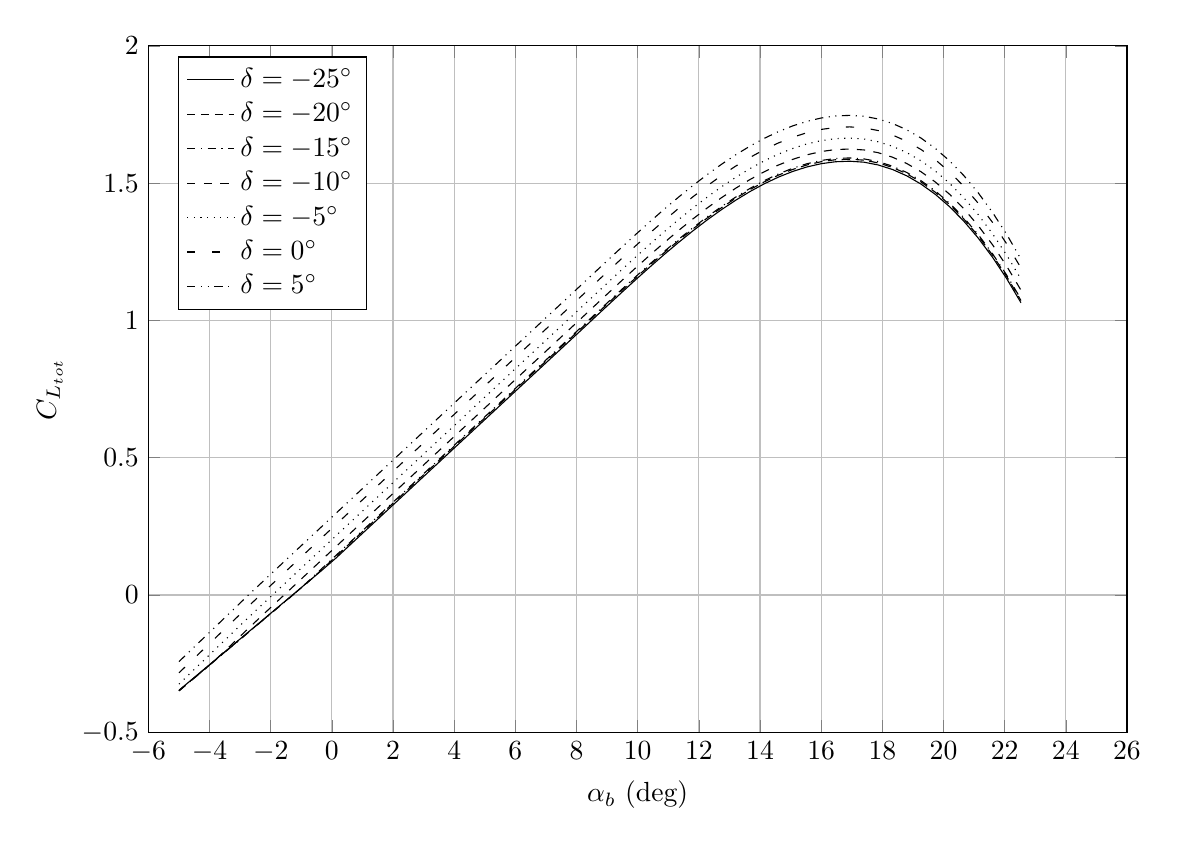
\begin{tikzpicture}

\begin{axis}[
width=14.01cm,
height=10.3cm,
scaled ticks=false, tick label style={/pgf/number format/fixed},
xmin=-6,
xmax=26,
xlabel={$\alpha_{b}$ (deg)},
xmajorgrids,
ymin=-0.5,
ymax=2,
ylabel={$C_{L_{tot}}$},
ymajorgrids,
legend style={at={(0.03,0.8)},anchor=west,draw=black,fill=white,legend cell align=left},
legend entries = {$\delta = -25^{\circ}$\\$\delta = -20^{\circ}$\\$\delta = -15^{\circ}$\\$\delta = -10^{\circ}$\\$\delta = -5^{\circ}$\\$\delta = 0^{\circ}$\\$\delta = 5^{\circ}$\\}
]

\addplot [
color=black,
solid
]
table[row sep=crcr]{
-4.999999999999999	-0.3471334642807813\\
-4.533333333333332	-0.30348056228561016\\
-4.0666666666666655	-0.25982766029043897\\
-3.5999999999999988	-0.2161747582952678\\
-3.133333333333332	-0.17252185630009662\\
-2.666666666666665	-0.12886895430492545\\
-2.1999999999999984	-0.08521605230975428\\
-1.7333333333333318	-0.0415631503145831\\
-1.2666666666666653	0.002089751680588031\\
-0.7999999999999987	0.04574265367575919\\
-0.33333333333333215	0.08939555567093033\\
0.13333333333333441	0.13452894861538855\\
0.600000000000001	0.18290195785697744\\
1.0666666666666675	0.23126601871175664\\
1.533333333333334	0.2796211006798399\\
2.000000000000001	0.32796717449147245\\
2.4666666666666677	0.3763042121373785\\
2.9333333333333345	0.4246320573011014\\
3.4000000000000012	0.47295052000316445\\
3.866666666666668	0.5212598681121062\\
4.333333333333335	0.5695600791928366\\
4.800000000000002	0.6178511322185285\\
5.266666666666668	0.666133007596158\\
5.733333333333335	0.7144056871911388\\
6.200000000000002	0.7626687582810414\\
6.666666666666669	0.8109225679034555\\
7.1333333333333355	0.8591671352258254\\
7.600000000000002	0.9074024484450889\\
8.066666666666668	0.9556657862020534\\
8.533333333333335	1.0041263356051073\\
9.000000000000002	1.0525552202017912\\
9.466666666666669	1.1006543008615628\\
9.933333333333335	1.1481216267630743\\
10.400000000000002	1.194655039253836\\
10.866666666666669	1.2399526030559629\\
11.333333333333336	1.2837126122711813\\
11.800000000000002	1.3256342965061445\\
12.26666666666667	1.365420409720979\\
12.733333333333336	1.4027674798153131\\
13.200000000000003	1.4373748874498455\\
13.66666666666667	1.4689423168233948\\
14.133333333333336	1.4971697782197084\\
14.600000000000003	1.5217576333181908\\
15.06666666666667	1.5424142285451603\\
15.533333333333337	1.5588373836265126\\
16.000000000000004	1.5707269236600594\\
16.46666666666667	1.5777850302039367\\
16.933333333333334	1.579714417097048\\
17.4	1.576173340338095\\
17.866666666666664	1.5660079314956457\\
18.33333333333333	1.5495175880459309\\
18.799999999999994	1.5263862930829049\\
19.26666666666666	1.49629802970052\\
19.733333333333324	1.4589367809927312\\
20.19999999999999	1.4139865300534933\\
20.666666666666654	1.3611312599767575\\
21.13333333333332	1.3000549538564796\\
21.599999999999984	1.2304415947866125\\
22.06666666666665	1.15197516586111\\
22.533333333333314	1.0643396501739297\\
};

\addplot [
color=black,
densely dashed
]
table[row sep=crcr]{
-4.999999999999999	-0.34809347859707673\\
-4.533333333333332	-0.3044405766019056\\
-4.0666666666666655	-0.26078767460673435\\
-3.5999999999999988	-0.21713477261156322\\
-3.133333333333332	-0.17348187061639203\\
-2.666666666666665	-0.12982896862122087\\
-2.1999999999999984	-0.0861760666260497\\
-1.7333333333333318	-0.04252316463087852\\
-1.2666666666666653	0.0011297373642926156\\
-0.7999999999999987	0.04478263935946378\\
-0.33333333333333215	0.09216878846158646\\
0.13333333333333441	0.14058588486816725\\
0.600000000000001	0.18899386968381748\\
1.0666666666666675	0.2373928398059092\\
1.533333333333334	0.28578276450855467\\
2.000000000000001	0.33416361430511293\\
2.4666666666666677	0.38253536097876195\\
2.9333333333333345	0.43089784705475404\\
3.4000000000000012	0.4792508811458815\\
3.866666666666668	0.5275947331055648\\
4.333333333333335	0.575929380332472\\
4.800000000000002	0.6242548016439691\\
5.266666666666668	0.6725709773018494\\
5.733333333333335	0.7208778890371511\\
6.200000000000002	0.7691751210692083\\
6.666666666666669	0.8174630230071281\\
7.1333333333333355	0.8657416141603842\\
7.600000000000002	0.9140108826384543\\
8.066666666666668	0.962308093029822\\
8.533333333333335	1.0108022601847622\\
9.000000000000002	1.059264561959493\\
9.466666666666669	1.1073969916961959\\
9.933333333333335	1.1548977028019565\\
10.400000000000002	1.2014646393127097\\
10.866666666666669	1.24679597029418\\
11.333333333333336	1.2905900958913858\\
11.800000000000002	1.332546358686281\\
12.26666666666667	1.3723676517294374\\
12.733333333333336	1.4097505958763759\\
13.200000000000003	1.444394685882392\\
13.66666666666667	1.4759997222900927\\
14.133333333333336	1.504265834143273\\
14.600000000000003	1.5288935044851966\\
15.06666666666667	1.5495912602723028\\
15.533333333333337	1.5660570237586975\\
16.000000000000004	1.5779907374300286\\
16.46666666666667	1.585094717693431\\
16.933333333333334	1.5870718171809577\\
17.4	1.5835801012558284\\
17.866666666666664	1.5734594930814727\\
18.33333333333333	1.5570139502998517\\
18.799999999999994	1.5339274560049194\\
19.26666666666666	1.5038839932906283\\
19.733333333333324	1.4665675452509332\\
20.19999999999999	1.4216620949797893\\
20.666666666666654	1.3688516255711474\\
21.13333333333332	1.3078201201189632\\
21.599999999999984	1.2382515617171899\\
22.06666666666665	1.159829933459781\\
22.533333333333314	1.0722392184406948\\
};

\addplot [
color=black,
dashdotted
]
table[row sep=crcr]{
-4.999999999999999	-0.3488170376822153\\
-4.533333333333332	-0.30516413568704415\\
-4.0666666666666655	-0.261511233691873\\
-3.5999999999999988	-0.21785833169670182\\
-3.133333333333332	-0.17420542970153063\\
-2.666666666666665	-0.13055252770635947\\
-2.1999999999999984	-0.0868996257111883\\
-1.7333333333333318	-0.04324672371601712\\
-1.2666666666666653	4.061782791540125E-4\\
-0.7999999999999987	0.04727738442691229\\
-0.33333333333333215	0.09573017751670179\\
0.13333333333333441	0.1441736853907836\\
0.600000000000001	0.19260803116162006\\
1.0666666666666675	0.24103331226375735\\
1.533333333333334	0.28944949780097134\\
2.000000000000001	0.3378565581231546\\
2.4666666666666677	0.38625446485705844\\
2.9333333333333345	0.43464305965493555\\
3.4000000000000012	0.48302215006857696\\
3.866666666666668	0.531392007447401\\
4.333333333333335	0.5797526090647798\\
4.800000000000002	0.6281039336206481\\
5.266666666666668	0.676445961267376\\
5.733333333333335	0.7247786736347229\\
6.200000000000002	0.773101652637042\\
6.666666666666669	0.8214152498215838\\
7.1333333333333355	0.8697194846048679\\
7.600000000000002	0.9180143450304548\\
8.066666666666668	0.966337085095645\\
8.533333333333335	1.0148565898204385\\
9.000000000000002	1.0633440779932937\\
9.466666666666669	1.1115016428005733\\
9.933333333333335	1.1590275162059307\\
10.400000000000002	1.2056197196411698\\
10.866666666666669	1.2509765008153908\\
11.333333333333336	1.2947963397980327\\
11.800000000000002	1.336778664320097\\
12.26666666666667	1.3766264722640877\\
12.733333333333336	1.4140364545460224\\
13.200000000000003	1.4487081919138551\\
13.66666666666667	1.480341572598056\\
14.133333333333336	1.5086368151514105\\
14.600000000000003	1.5332944940886537\\
15.06666666666667	1.554023272431081\\
15.533333333333337	1.5705211497079143\\
16.000000000000004	1.5824881568795615\\
16.46666666666667	1.5896267119883254\\
16.933333333333334	1.5916397722741227\\
17.4	1.5881852594189443\\
17.866666666666664	1.5780984173352284\\
18.33333333333333	1.5616866406442473\\
18.799999999999994	1.5386339124399546\\
19.26666666666666	1.5086242158163035\\
19.733333333333324	1.4713415338672482\\
20.19999999999999	1.426469849686744\\
20.666666666666654	1.3736931463687418\\
21.13333333333332	1.3126954070071974\\
21.599999999999984	1.243160614696064\\
22.06666666666665	1.164772752529295\\
22.533333333333314	1.0772158036008486\\
};

\addplot [
color=black,
dashed
]
table[row sep=crcr]{
-4.999999999999999	-0.34926252296465465\\
-4.533333333333332	-0.3056096209694835\\
-4.0666666666666655	-0.26195671897431233\\
-3.5999999999999988	-0.21452739910285312\\
-3.133333333333332	-0.1647290942219834\\
-2.666666666666665	-0.11493078934111371\\
-2.1999999999999984	-0.0663085684658876\\
-1.7333333333333318	-0.01781261672903274\\
-1.2666666666666653	0.030674416274122956\\
-0.7999999999999987	0.07915249359905727\\
-0.33333333333333215	0.12762157938029853\\
0.13333333333333441	0.17608134842820983\\
0.600000000000001	0.2245319242731449\\
1.0666666666666675	0.27297340468038056\\
1.533333333333334	0.3214057586488189\\
2.000000000000001	0.3698289564277086\\
2.4666666666666677	0.418242969547491\\
2.9333333333333345	0.46664763912292534\\
3.4000000000000012	0.5150427720525587\\
3.866666666666668	0.5634286406068746\\
4.333333333333335	0.611805221982102\\
4.800000000000002	0.6601724948058754\\
5.266666666666668	0.7085304391631938\\
5.733333333333335	0.7568790366214613\\
6.200000000000002	0.8052178676758861\\
6.666666666666669	0.8535472850670062\\
7.1333333333333355	0.9018673082772489\\
7.600000000000002	0.9501779253095894\\
8.066666666666668	0.9985163836404846\\
8.533333333333335	1.0470514883552364\\
9.000000000000002	1.0955544834437156\\
9.466666666666669	1.1437275235649602\\
9.933333333333335	1.1912688890488128\\
10.400000000000002	1.2378766489786384\\
10.866666666666669	1.283249099483172\\
11.333333333333336	1.3270847698402084\\
11.800000000000002	1.3690831402058359\\
12.26666666666667	1.4089472730061234\\
12.733333333333336	1.4463739022923634\\
13.200000000000003	1.4810626617569957\\
13.66666666666667	1.5127134936186908\\
14.133333333333336	1.5410266715396763\\
14.600000000000003	1.5657028263524022\\
15.06666666666667	1.5864507048514072\\
15.533333333333337	1.6029683541431285\\
16.000000000000004	1.6149558596606552\\
16.46666666666667	1.622115702021653\\
16.933333333333334	1.6241509028716465\\
17.4	1.6207192954300895\\
17.866666666666664	1.6106532426595543\\
18.33333333333333	1.5942622552817536\\
18.799999999999994	1.5712303163906416\\
19.26666666666666	1.5412414090801707\\
19.733333333333324	1.503979516444296\\
20.19999999999999	1.4591286215769723\\
20.666666666666654	1.4063727075721508\\
21.13333333333332	1.345395757523787\\
21.599999999999984	1.2758817545258339\\
22.06666666666665	1.1975150647626562\\
22.533333333333314	1.1099837594215713\\
};

\addplot [
color=black,
dotted
]
table[row sep=crcr]{
-4.999999999999999	-0.3244319352636276\\
-4.533333333333332	-0.27462653684686594\\
-4.0666666666666655	-0.2248211384301042\\
-3.5999999999999988	-0.17501574001334247\\
-3.133333333333332	-0.12521034159658076\\
-2.666666666666665	-0.07540494317981904\\
-2.1999999999999984	-0.026776986302822173\\
-1.7333333333333318	0.021724555685446373\\
-1.2666666666666653	0.07021716864527042\\
-0.7999999999999987	0.11870081558948332\\
-0.33333333333333215	0.1671754606112145\\
0.13333333333333441	0.21564077814546603\\
0.600000000000001	0.26409689186518076\\
1.0666666666666675	0.3125438996484842\\
1.533333333333334	0.36098177045849456\\
2.000000000000001	0.40941047451011964\\
2.4666666666666677	0.4578299833009388\\
2.9333333333333345	0.5062401377623128\\
3.4000000000000012	0.5546407445698949\\
3.866666666666668	0.6030320763084458\\
4.333333333333335	0.6514141101478725\\
4.800000000000002	0.6997868246911397\\
5.266666666666668	0.7481502000002591\\
5.733333333333335	0.796504217621358\\
6.200000000000002	0.8448484575654175\\
6.666666666666669	0.893183272980138\\
7.1333333333333355	0.941508683370435\\
7.600000000000002	0.9898246767254357\\
8.066666666666668	1.0381684982966155\\
8.533333333333335	1.0867089258947027\\
9.000000000000002	1.1352172121085595\\
9.466666666666669	1.1833955325723582\\
9.933333333333335	1.2309421841190011\\
10.400000000000002	1.2775552520910762\\
10.866666666666669	1.3229330491386155\\
11.333333333333336	1.3667741213298308\\
11.800000000000002	1.4087779667088096\\
12.26666666666667	1.448647669724576\\
12.733333333333336	1.4860799791466393\\
13.200000000000003	1.5207745467326634\\
13.66666666666667	1.55243133312267\\
14.133333333333336	1.5807506307828176\\
14.600000000000003	1.605433089761763\\
15.06666666666667	1.62618748543837\\
15.533333333333337	1.6427118811529313\\
16.000000000000004	1.6547063809251965\\
16.46666666666667	1.6618734867242142\\
16.933333333333334	1.663916242171391\\
17.4	1.6604924503018172\\
17.866666666666664	1.650433491067174\\
18.33333333333333	1.6340495972252653\\
18.799999999999994	1.6110247518700453\\
19.26666666666666	1.5810442070983473\\
19.733333333333324	1.5438016322567218\\
20.19999999999999	1.4989879437214455\\
20.666666666666654	1.4462922754288399\\
21.13333333333332	1.385404525410811\\
21.599999999999984	1.316006817419822\\
22.06666666666665	1.237767791199569\\
22.533333333333314	1.1503603439426384\\
};

\addplot [
color=black,
loosely dashed
]
table[row sep=crcr]{
-4.999999999999999	-0.2834224286758397\\
-4.533333333333332	-0.23362379637622757\\
-4.0666666666666655	-0.18382516407661537\\
-3.5999999999999988	-0.1340265317770032\\
-3.133333333333332	-0.08422789947739097\\
-2.666666666666665	-0.03442926717777879\\
-2.1999999999999984	0.014193218456026838\\
-1.7333333333333318	0.06268942822401258\\
-1.2666666666666653	0.11117671878312106\\
-0.7999999999999987	0.1596550531868618\\
-0.33333333333333215	0.20812439556785217\\
0.13333333333333441	0.2565844207191297\\
0.600000000000001	0.3050352521776295\\
1.0666666666666675	0.35347698771383734\\
1.533333333333334	0.4019095963250036\\
2.000000000000001	0.4503330482587918\\
2.4666666666666677	0.49874731504412656\\
2.9333333333333345	0.5471522377873018\\
3.4000000000000012	0.5955476233765765\\
3.866666666666668	0.6439337440969405\\
4.333333333333335	0.6923105771434075\\
4.800000000000002	0.7406781011424735\\
5.266666666666668	0.7890362961780766\\
5.733333333333335	0.8373851438166384\\
6.200000000000002	0.885724224531017\\
6.666666666666669	0.9340538910805436\\
7.1333333333333355	0.9823741629486836\\
7.600000000000002	1.0306850281377729\\
8.066666666666668	1.0790237340215691\\
8.533333333333335	1.1275590844264527\\
9.000000000000002	1.176062323739201\\
9.466666666666669	1.224235607587008\\
9.933333333333335	1.2717772170614539\\
10.400000000000002	1.3183852219963863\\
10.866666666666669	1.363757919283119\\
11.333333333333336	1.4075938389744482\\
11.800000000000002	1.449592462052124\\
12.26666666666667	1.489456851958737\\
12.733333333333336	1.5268837434249332\\
13.200000000000003	1.5615727709769949\\
13.66666666666667	1.5932238776838732\\
14.133333333333336	1.621537338075735\\
14.600000000000003	1.6462137838719997\\
15.06666666666667	1.6669619631865822\\
15.533333333333337	1.6834799247345416\\
16.000000000000004	1.695467757236948\\
16.46666666666667	1.702633225232\\
16.933333333333334	1.7046923343976499\\
17.4	1.7013142161255614\\
17.866666666666664	1.6913259327158507\\
18.33333333333333	1.6750427979851077\\
18.799999999999994	1.652150300389209\\
19.26666666666666	1.62231255757573\\
19.733333333333324	1.585202105480899\\
20.19999999999999	1.5404899804325125\\
20.666666666666654	1.4878295406937958\\
21.13333333333332	1.4268681417494065\\
21.599999999999984	1.35726945946871\\
22.06666666666665	1.2786900491053128\\
22.533333333333314	1.1907795747314511\\
};

\addplot [
color=black,
dashdotdotted
]
table[row sep=crcr]{
-4.999999999999999	-0.24255791031268456\\
-4.533333333333332	-0.19275251189592288\\
-4.0666666666666655	-0.14294711347916114\\
-3.5999999999999988	-0.09314171506239942\\
-3.133333333333332	-0.04333631664563769\\
-2.666666666666665	0.006469081771124018\\
-2.1999999999999984	0.055097038648120884\\
-1.7333333333333318	0.10359858063638944\\
-1.2666666666666653	0.15209119359621348\\
-0.7999999999999987	0.2005748405404264\\
-0.33333333333333215	0.24904948556215756\\
0.13333333333333441	0.2975148030964091\\
0.600000000000001	0.3459709168161238\\
1.0666666666666675	0.3944179245994273\\
1.533333333333334	0.44285579540943765\\
2.000000000000001	0.4912844994610627\\
2.4666666666666677	0.5397040082518819\\
2.9333333333333345	0.5881141627132559\\
3.4000000000000012	0.636514769520838\\
3.866666666666668	0.6849061012593889\\
4.333333333333335	0.7332881350988156\\
4.800000000000002	0.7816608496420828\\
5.266666666666668	0.8300242249512021\\
5.733333333333335	0.878378242572301\\
6.200000000000002	0.9267224825163605\\
6.666666666666669	0.975057297931081\\
7.1333333333333355	1.023382708321378\\
7.600000000000002	1.0716987016763788\\
8.066666666666668	1.1200425232475586\\
8.533333333333335	1.1685829508456458\\
9.000000000000002	1.2170912370595026\\
9.466666666666669	1.2652695575233013\\
9.933333333333335	1.3128162090699442\\
10.400000000000002	1.3594292770420193\\
10.866666666666669	1.4048070740895586\\
11.333333333333336	1.4486481462807739\\
11.800000000000002	1.4906519916597527\\
12.26666666666667	1.530521842806712\\
12.733333333333336	1.567954529792535\\
13.200000000000003	1.602657567157949\\
13.66666666666667	1.6343312135643657\\
14.133333333333336	1.662689623299419\\
14.600000000000003	1.6874395803177127\\
15.06666666666667	1.7082862101768348\\
15.533333333333337	1.7249358885552355\\
16.000000000000004	1.7370915466347452\\
16.46666666666667	1.7444392740312173\\
16.933333333333334	1.7466717428638403\\
17.4	1.7434256761774112\\
17.866666666666664	1.7334870405721827\\
18.33333333333333	1.7171347362357516\\
18.799999999999994	1.6940374819607558\\
19.26666666666666	1.663852771203165\\
19.733333333333324	1.6262370122158905\\
20.19999999999999	1.580737911763286\\
20.666666666666654	1.527055161402033\\
21.13333333333332	1.464838521628392\\
21.599999999999984	1.3937314207732419\\
22.06666666666665	1.3132585213316923\\
22.533333333333314	1.2230296402460932\\
};
\end{axis}
\end{tikzpicture}%

\caption{ATR 72 . Mach 0.45. $CL_{tot}$ vs $\alpha_b$ with elevator deflections.}
\label{fig:stallATR}
\end{figure}
\begin{figure}[H]
\centering
%Comparison of CD estimation
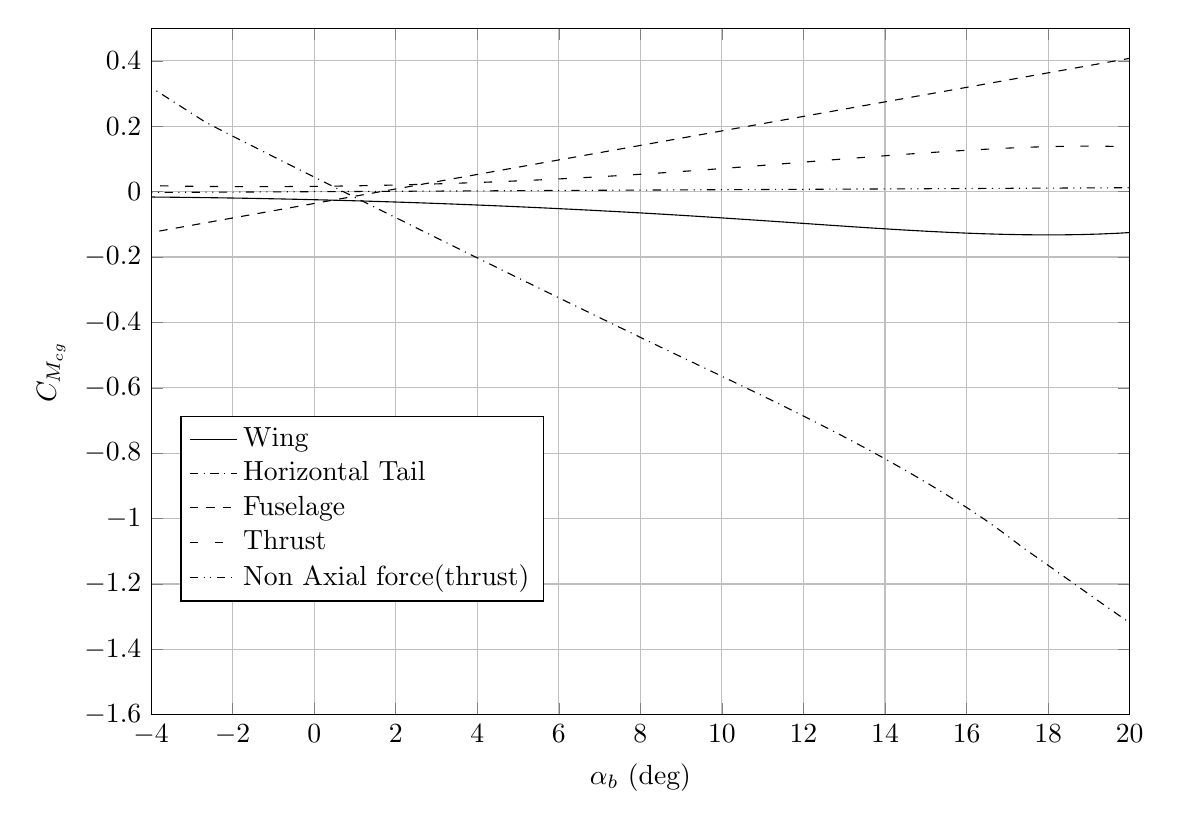
\begin{tikzpicture}

\begin{axis}[
width=14.01cm,
height=10.3cm,
scaled ticks=false, tick label style={/pgf/number format/fixed},
xmin=-4,
xmax=20,
xlabel={$\alpha_{b}$ (deg)},
xmajorgrids,
ymin=-1.6,
ymax=0.5,
ylabel={$C_{M_{cg}}$},
ymajorgrids,
legend style={at={(0.03,0.3)},anchor=west,draw=black,fill=white,legend cell align=left},
legend entries = {Wing\\Horizontal Tail \\Fuselage\\Thrust\\Non Axial force(thrust)\\}
]

\addplot [
color=black,
solid
]
table[row sep=crcr]{
-4.999999999999999	-0.015557992842992079\\
-4.533333333333332	-0.015865801553338287\\
-4.0666666666666655	-0.01628640497169006\\
-3.5999999999999988	-0.01681411998510184\\
-3.133333333333332	-0.017454037765245373\\
-2.666666666666665	-0.018201306335162228\\
-2.1999999999999984	-0.0190601788043208\\
-1.7333333333333318	-0.02002663268361221\\
-1.2666666666666653	-0.021104084902447556\\
-0.7999999999999987	-0.02228934238407632\\
-0.33333333333333215	-0.023584986500966108\\
0.13333333333333441	-0.024988649508308813\\
0.600000000000001	-0.026502080067522422\\
1.0666666666666675	-0.028123750088813508\\
1.533333333333334	-0.02985454490646395\\
2.000000000000001	-0.03169375388039104\\
2.4666666666666677	-0.03364146789772598\\
2.9333333333333345	-0.03569777322143715\\
3.4000000000000012	-0.03786193692252439\\
3.866666666666668	-0.04013485319754568\\
4.333333333333335	-0.04251496953308821\\
4.800000000000002	-0.04500398070437446\\
5.266666666666668	-0.047599519264004936\\
5.733333333333335	-0.05030407371906394\\
6.200000000000002	-0.05311446705337142\\
6.666666666666669	-0.05603397366519865\\
7.1333333333333355	-0.05905861302029114\\
7.600000000000002	-0.062192436939615806\\
8.066666666666668	-0.06543066809478415\\
8.533333333333335	-0.06879838315839079\\
9.000000000000002	-0.07231166953099327\\
9.466666666666669	-0.07595578595257153\\
9.933333333333335	-0.07970186344358024\\
10.400000000000002	-0.08352944145693766\\
10.866666666666669	-0.0874106441364871\\
11.333333333333336	-0.09135438573117291\\
11.800000000000002	-0.0953496322008784\\
12.26666666666667	-0.09935802355381973\\
12.733333333333336	-0.10334267762953267\\
13.200000000000003	-0.10726013879538575\\
13.66666666666667	-0.11106986821231829\\
14.133333333333336	-0.11472392678841327\\
14.600000000000003	-0.11817734072286938\\
15.06666666666667	-0.1213782433617562\\
15.533333333333337	-0.12427610306818715\\
16.000000000000004	-0.12681593462459115\\
16.46666666666667	-0.12894187275403707\\
16.933333333333334	-0.13059499980214567\\
17.4	-0.13171378843855064\\
17.866666666666664	-0.13223682601742598\\
18.33333333333333	-0.13209684167872648\\
18.799999999999994	-0.13122955850193516\\
19.26666666666666	-0.12956193614454592\\
19.733333333333324	-0.12702671594225018\\
20.19999999999999	-0.12354534261450884\\
20.666666666666654	-0.1190480667547701\\
21.13333333333332	-0.11345108010375851\\
21.599999999999984	-0.10668181811603417\\
22.06666666666665	-0.09865158802340677\\
22.533333333333314	-0.08928483557214614\\
22.999999999999993	-0.0784884775363909\\
};
\addplot [
color=black,
dashdotted
]
table[row sep=crcr]{
-4.999999999999999	0.39867051253373126\\
-4.533333333333332	0.3614612646972497\\
-4.0666666666666655	0.3242520168607681\\
-3.5999999999999988	0.2870427690242865\\
-3.133333333333332	0.24983352118780489\\
-2.666666666666665	0.21262427335132328\\
-2.1999999999999984	0.18253599090253916\\
-1.7333333333333318	0.15321224411580053\\
-1.2666666666666653	0.12394249856848781\\
-0.7999999999999987	0.0947269779526696\\
-0.33333333333333215	0.06556589942696817\\
0.13333333333333441	0.03646123195290178\\
0.600000000000001	0.007412227577628631\\
1.0666666666666675	-0.021581705649042257\\
1.533333333333334	-0.05052038002134837\\
2.000000000000001	-0.07940361540413787\\
2.4666666666666677	-0.10823123941963848\\
2.9333333333333345	-0.13700229004787956\\
3.4000000000000012	-0.16571559809622144\\
3.866666666666668	-0.19437281211075622\\
4.333333333333335	-0.22297379401897602\\
4.800000000000002	-0.2515184144152667\\
5.266666666666668	-0.28000655271808017\\
5.733333333333335	-0.3084380973215431\\
6.200000000000002	-0.3368105082037837\\
6.666666666666669	-0.36512592114179115\\
7.1333333333333355	-0.39338445409796924\\
7.600000000000002	-0.4215860344326079\\
8.066666666666668	-0.4497189909711484\\
8.533333333333335	-0.47764025453404557\\
9.000000000000002	-0.5053949312577264\\
9.466666666666669	-0.5330930465191119\\
9.933333333333335	-0.5608211673673333\\
10.400000000000002	-0.5886645817942104\\
10.866666666666669	-0.6167099525081683\\
11.333333333333336	-0.6450453538909372\\
11.800000000000002	-0.6737646177117909\\
12.26666666666667	-0.7029832657046937\\
12.733333333333336	-0.7327785024956976\\
13.200000000000003	-0.7632450894875461\\
13.66666666666667	-0.7944796561507343\\
14.133333333333336	-0.8265808387835795\\
14.600000000000003	-0.8596494362822812\\
15.06666666666667	-0.8938353881527763\\
15.533333333333337	-0.9292238493207469\\
16.000000000000004	-0.9659129629825098\\
16.46666666666667	-1.0047466503260158\\
16.933333333333334	-1.0464129237254836\\
17.4	-1.0905805709197096\\
17.866666666666664	-1.131334400568644\\
18.33333333333333	-1.1724723684836247\\
18.799999999999994	-1.2137525247123828\\
19.26666666666666	-1.254932919302652\\
19.733333333333324	-1.2957716023021644\\
20.19999999999999	-1.3360266237586522\\
20.666666666666654	-1.375456033719848\\
21.13333333333332	-1.4138178822334835\\
21.599999999999984	-1.4508702193472924\\
22.06666666666665	-1.486371095109007\\
22.533333333333314	-1.5200785595663588\\
22.999999999999993	-1.5517506627670823\\
};

\addplot [
color=black,
dashed
]
table[row sep=crcr]{
-4.999999999999999	-0.14709999999999998\\
-4.533333333333332	-0.13673999999999997\\
-4.0666666666666655	-0.12638\\
-3.5999999999999988	-0.11601999999999998\\
-3.133333333333332	-0.10565999999999998\\
-2.666666666666665	-0.09529999999999997\\
-2.1999999999999984	-0.08493999999999996\\
-1.7333333333333318	-0.07457999999999997\\
-1.2666666666666653	-0.06421999999999997\\
-0.7999999999999987	-0.05385999999999998\\
-0.33333333333333215	-0.043499999999999976\\
0.13333333333333441	-0.033139999999999975\\
0.600000000000001	-0.022779999999999977\\
1.0666666666666675	-0.01241999999999998\\
1.533333333333334	-0.0020599999999999785\\
2.000000000000001	0.008300000000000023\\
2.4666666666666677	0.018660000000000024\\
2.9333333333333345	0.029020000000000025\\
3.4000000000000012	0.03938000000000003\\
3.866666666666668	0.04974000000000003\\
4.333333333333335	0.060100000000000035\\
4.800000000000002	0.07046000000000005\\
5.266666666666668	0.08082000000000003\\
5.733333333333335	0.09118000000000007\\
6.200000000000002	0.10154000000000005\\
6.666666666666669	0.11190000000000005\\
7.1333333333333355	0.12226000000000006\\
7.600000000000002	0.13262000000000007\\
8.066666666666668	0.14298000000000005\\
8.533333333333335	0.15334000000000006\\
9.000000000000002	0.16370000000000007\\
9.466666666666669	0.17406000000000005\\
9.933333333333335	0.18442000000000006\\
10.400000000000002	0.19478000000000006\\
10.866666666666669	0.20514000000000007\\
11.333333333333336	0.21550000000000005\\
11.800000000000002	0.2258600000000001\\
12.26666666666667	0.23622000000000007\\
12.733333333333336	0.2465800000000001\\
13.200000000000003	0.25694000000000006\\
13.66666666666667	0.26730000000000004\\
14.133333333333336	0.2776600000000001\\
14.600000000000003	0.28802000000000005\\
15.06666666666667	0.2983800000000001\\
15.533333333333337	0.30874000000000007\\
16.000000000000004	0.31910000000000005\\
16.46666666666667	0.32946000000000003\\
16.933333333333334	0.33982\\
17.4	0.35018\\
17.866666666666664	0.3605399999999999\\
18.33333333333333	0.3708999999999999\\
18.799999999999994	0.3812599999999999\\
19.26666666666666	0.3916199999999998\\
19.733333333333324	0.4019799999999998\\
20.19999999999999	0.41233999999999976\\
20.666666666666654	0.4226999999999997\\
21.13333333333332	0.43305999999999967\\
21.599999999999984	0.44341999999999965\\
22.06666666666665	0.45377999999999963\\
22.533333333333314	0.46413999999999955\\
22.999999999999993	0.4744999999999998\\
};

\addplot [
color=black,
loosely dashed
]
table[row sep=crcr]{
-4.999999999999999	0.021570650822018575\\
-4.533333333333332	0.02000085813112243\\
-4.0666666666666655	0.01865836770621552\\
-3.5999999999999988	0.01754317954729784\\
-3.133333333333332	0.016655293654369397\\
-2.666666666666665	0.015994710027430182\\
-2.1999999999999984	0.01558802739674183\\
-1.7333333333333318	0.015374490889257325\\
-1.2666666666666653	0.015349312614196082\\
-0.7999999999999987	0.015512111279939688\\
-0.33333333333333215	0.015862503788633207\\
0.13333333333333441	0.016400091428762382\\
0.600000000000001	0.017124485122131633\\
1.0666666666666675	0.018035301111729008\\
1.533333333333334	0.019132149819020255\\
2.000000000000001	0.020414640307694288\\
2.4666666666666677	0.021882380378802795\\
2.9333333333333345	0.02353495917733285\\
3.4000000000000012	0.02537195211664482\\
3.866666666666668	0.02739299892408932\\
4.333333333333335	0.029597703306433933\\
4.800000000000002	0.031985668232490064\\
5.266666666666668	0.034556496041477015\\
5.733333333333335	0.037309788553168174\\
6.200000000000002	0.040245054004529886\\
6.666666666666669	0.04336196691712855\\
7.1333333333333355	0.046660135440486104\\
7.600000000000002	0.05013916049156789\\
8.066666666666668	0.05380025812934947\\
8.533333333333335	0.05764730226375402\\
9.000000000000002	0.061668710038886146\\
9.466666666666669	0.06584924845051271\\
9.933333333333335	0.07016999185035566\\
10.400000000000002	0.07460940790244441\\
10.866666666666669	0.07914357608206717\\
11.333333333333336	0.08374629902113512\\
11.800000000000002	0.08838951870393907\\
12.26666666666667	0.0930445903785934\\
12.733333333333336	0.09767848526601111\\
13.200000000000003	0.1022575783643235\\
13.66666666666667	0.10674687405443531\\
14.133333333333336	0.11111025551761636\\
14.600000000000003	0.11531075585211142\\
15.06666666666667	0.11931450565190461\\
15.533333333333337	0.12308230128084671\\
16.000000000000004	0.12657571431718476\\
16.46666666666667	0.1298175489827388\\
16.933333333333334	0.1328212381998705\\
17.4	0.13551709013128246\\
17.866666666666664	0.1373612142352387\\
18.33333333333333	0.1386250962400392\\
18.799999999999994	0.1392475838403341\\
19.26666666666666	0.13917180946090257\\
19.733333333333324	0.13834660241499672\\
20.19999999999999	0.13672801015634486\\
20.666666666666654	0.13428092862481694\\
21.13333333333332	0.13098084168575044\\
21.599999999999984	0.12681566966293698\\
22.06666666666665	0.12178772696526956\\
22.533333333333314	0.11591578880705147\\
22.999999999999993	0.10923726702196387\\
};

\addplot [
color=black,
dashdotdotted
]
table[row sep=crcr]{
-4.999999999999999	-0.003015548189021825\\
-4.533333333333332	-0.002734097024713121\\
-4.0666666666666655	-0.0024526458604044172\\
-3.5999999999999988	-0.0021711946960957136\\
-3.133333333333332	-0.0018897435317870095\\
-2.666666666666665	-0.001608292367478306\\
-2.1999999999999984	-0.001326841203169602\\
-1.7333333333333318	-0.0010453900388608984\\
-1.2666666666666653	-7.639388745521949E-4\\
-0.7999999999999987	-4.824877102434913E-4\\
-0.33333333333333215	-2.0103654593478764E-4\\
0.13333333333333441	8.0414618373916E-5\\
0.600000000000001	3.618657826826196E-4\\
1.0666666666666675	6.433169469913233E-4\\
1.533333333333334	9.247681113000269E-4\\
2.000000000000001	0.0012062192756087306\\
2.4666666666666677	0.0014876704399174343\\
2.9333333333333345	0.0017691216042261381\\
3.4000000000000012	0.0020505727685348417\\
3.866666666666668	0.002332023932843546\\
4.333333333333335	0.0026134750971522494\\
4.800000000000002	0.002894926261460953\\
5.266666666666668	0.003176377425769657\\
5.733333333333335	0.0034578285900783608\\
6.200000000000002	0.0037392797543870644\\
6.666666666666669	0.004020730918695769\\
7.1333333333333355	0.004302182083004472\\
7.600000000000002	0.004583633247313176\\
8.066666666666668	0.004865084411621879\\
8.533333333333335	0.005146535575930583\\
9.000000000000002	0.005427986740239287\\
9.466666666666669	0.00570943790454799\\
9.933333333333335	0.005990889068856695\\
10.400000000000002	0.006272340233165398\\
10.866666666666669	0.006553791397474101\\
11.333333333333336	0.006835242561782805\\
11.800000000000002	0.007116693726091509\\
12.26666666666667	0.007398144890400213\\
12.733333333333336	0.0076795960547089166\\
13.200000000000003	0.00796104721901762\\
13.66666666666667	0.008242498383326325\\
14.133333333333336	0.008523949547635029\\
14.600000000000003	0.008805400711943731\\
15.06666666666667	0.009086851876252437\\
15.533333333333337	0.00936830304056114\\
16.000000000000004	0.009649754204869843\\
16.46666666666667	0.009931205369178546\\
16.933333333333334	0.010212656533487248\\
17.4	0.01049410769779595\\
17.866666666666664	0.010775558862104653\\
18.33333333333333	0.011057010026413358\\
18.799999999999994	0.01133846119072206\\
19.26666666666666	0.011619912355030763\\
19.733333333333324	0.011901363519339465\\
20.19999999999999	0.012182814683648168\\
20.666666666666654	0.01246426584795687\\
21.13333333333332	0.012745717012265572\\
21.599999999999984	0.013027168176574275\\
22.06666666666665	0.013308619340882979\\
22.533333333333314	0.013590070505191681\\
22.999999999999993	0.013871521669500392\\
};
\end{axis}
\end{tikzpicture}%

\caption{ATR 72 . Mach 0.45. CM respect to CG vs $\alpha_b$ of aircraft's components.}
\label{fig:stallATR}
\end{figure}
\begin{figure}[H]
\centering
%Comparison of CD estimation
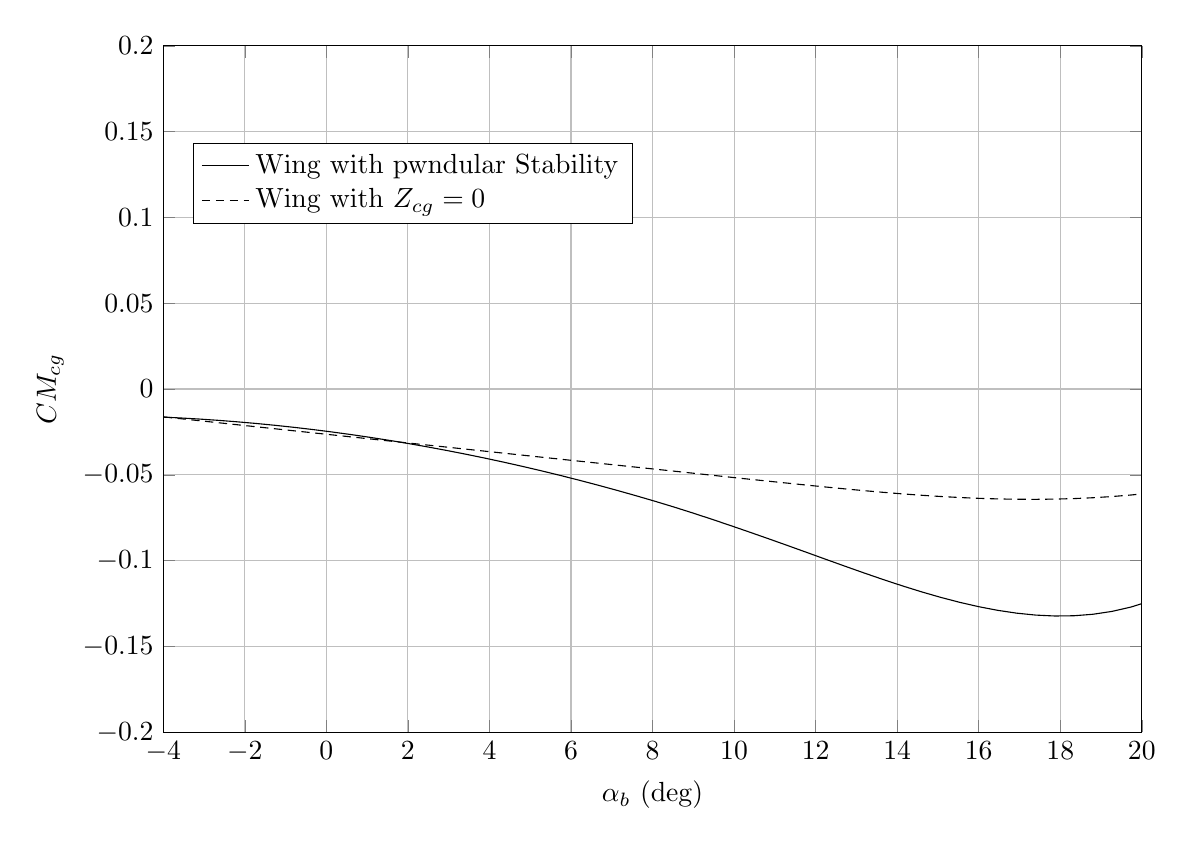
\begin{tikzpicture}

\begin{axis}[
width=14.01cm,
height=10.3cm,
scaled ticks=false, tick label style={/pgf/number format/fixed},
xmin=-4,
xmax=20,
xlabel={$\alpha_{b}$ (deg)},
xmajorgrids,
ymin=-0.2,
ymax=0.2,
ylabel={$CM_{cg}$},
ymajorgrids,
legend style={at={(0.03,0.8)},anchor=west,draw=black,fill=white,legend cell align=left},
legend entries = {Wing with pwndular Stability \\ Wing with $Z_{cg}=0$\\}
]

\addplot [
color=black,
solid
]
table[row sep=crcr]{
-4.999999999999999	-0.015557992842992079\\
-4.533333333333332	-0.015865801553338287\\
-4.0666666666666655	-0.01628640497169006\\
-3.5999999999999988	-0.01681411998510184\\
-3.133333333333332	-0.017454037765245373\\
-2.666666666666665	-0.018201306335162228\\
-2.1999999999999984	-0.0190601788043208\\
-1.7333333333333318	-0.02002663268361221\\
-1.2666666666666653	-0.021104084902447556\\
-0.7999999999999987	-0.02228934238407632\\
-0.33333333333333215	-0.023584986500966108\\
0.13333333333333441	-0.024988649508308813\\
0.600000000000001	-0.026502080067522422\\
1.0666666666666675	-0.028123750088813508\\
1.533333333333334	-0.02985454490646395\\
2.000000000000001	-0.03169375388039104\\
2.4666666666666677	-0.03364146789772598\\
2.9333333333333345	-0.03569777322143715\\
3.4000000000000012	-0.03786193692252439\\
3.866666666666668	-0.04013485319754568\\
4.333333333333335	-0.04251496953308821\\
4.800000000000002	-0.04500398070437446\\
5.266666666666668	-0.047599519264004936\\
5.733333333333335	-0.05030407371906394\\
6.200000000000002	-0.05311446705337142\\
6.666666666666669	-0.05603397366519865\\
7.1333333333333355	-0.05905861302029114\\
7.600000000000002	-0.062192436939615806\\
8.066666666666668	-0.06543066809478415\\
8.533333333333335	-0.06879838315839079\\
9.000000000000002	-0.07231166953099327\\
9.466666666666669	-0.07595578595257153\\
9.933333333333335	-0.07970186344358024\\
10.400000000000002	-0.08352944145693766\\
10.866666666666669	-0.0874106441364871\\
11.333333333333336	-0.09135438573117291\\
11.800000000000002	-0.0953496322008784\\
12.26666666666667	-0.09935802355381973\\
12.733333333333336	-0.10334267762953267\\
13.200000000000003	-0.10726013879538575\\
13.66666666666667	-0.11106986821231829\\
14.133333333333336	-0.11472392678841327\\
14.600000000000003	-0.11817734072286938\\
15.06666666666667	-0.1213782433617562\\
15.533333333333337	-0.12427610306818715\\
16.000000000000004	-0.12681593462459115\\
16.46666666666667	-0.12894187275403707\\
16.933333333333334	-0.13059499980214567\\
17.4	-0.13171378843855064\\
17.866666666666664	-0.13223682601742598\\
18.33333333333333	-0.13209684167872648\\
18.799999999999994	-0.13122955850193516\\
19.26666666666666	-0.12956193614454592\\
19.733333333333324	-0.12702671594225018\\
20.19999999999999	-0.12354534261450884\\
20.666666666666654	-0.1190480667547701\\
21.13333333333332	-0.11345108010375851\\
21.599999999999984	-0.10668181811603417\\
22.06666666666665	-0.09865158802340677\\
22.533333333333314	-0.08928483557214614\\
22.999999999999993	-0.0784884775363909\\
};

\addplot [
color=black,
densely dashed
]
table[row sep=crcr]{
-4.999999999999999	-0.013667947222667034\\
-4.533333333333332	-0.014846650426633762\\
-4.0666666666666655	-0.01602659231294674\\
-3.5999999999999988	-0.017207580025289132\\
-3.133333333333332	-0.018389527306312752\\
-2.666666666666665	-0.01957226069590415\\
-2.1999999999999984	-0.020755676553758897\\
-1.7333333333333318	-0.021939617005612203\\
-1.2666666666666653	-0.0231239646605842\\
-0.7999999999999987	-0.024308573421791387\\
-0.33333333333333215	-0.025493315772200917\\
0.13333333333333441	-0.026678053567844952\\
0.600000000000001	-0.027862652809703868\\
1.0666666666666675	-0.029046996356507405\\
1.533333333333334	-0.030230914473788114\\
2.000000000000001	-0.03141428950779003\\
2.4666666666666677	-0.032596985440895405\\
2.9333333333333345	-0.03377886510858846\\
3.4000000000000012	-0.03495979697646863\\
3.866666666666668	-0.03613963660639739\\
4.333333333333335	-0.03731826061612875\\
4.800000000000002	-0.038495513526399266\\
5.266666666666668	-0.0396712837869202\\
5.733333333333335	-0.040845401121134745\\
6.200000000000002	-0.04201776949379599\\
6.666666666666669	-0.04318820009805835\\
7.1333333333333355	-0.044356616098977716\\
7.600000000000002	-0.04552280644918972\\
8.066666666666668	-0.046686717199235665\\
8.533333333333335	-0.04785786025984706\\
9.000000000000002	-0.04904551828968284\\
9.466666666666669	-0.050238709349704536\\
9.933333333333335	-0.05142651144454903\\
10.400000000000002	-0.05259780381965731\\
10.866666666666669	-0.05374442905276344\\
11.333333333333336	-0.054882034813226704\\
11.800000000000002	-0.05601360861841795\\
12.26666666666667	-0.05712463580135882\\
12.733333333333336	-0.05820083288107426\\
13.200000000000003	-0.05922884462427676\\
13.66666666666667	-0.06019565619623717\\
14.133333333333336	-0.06108841743832603\\
14.600000000000003	-0.06189502577379964\\
15.06666666666667	-0.06260313352006822\\
15.533333333333337	-0.06320061424103503\\
16.000000000000004	-0.0636761586733407\\
16.46666666666667	-0.0640182905630333\\
16.933333333333334	-0.06421500203784317\\
17.4	-0.0642552860064942\\
17.866666666666664	-0.0641282812554299\\
18.33333333333333	-0.06382346658092841\\
18.799999999999994	-0.06333025405578231\\
19.26666666666666	-0.06263839083572617\\
19.733333333333324	-0.06173688243701636\\
20.19999999999999	-0.0606160066339696\\
20.666666666666654	-0.05926574565099551\\
21.13333333333332	-0.05767694481506007\\
21.599999999999984	-0.055839932505489416\\
22.06666666666665	-0.0537460691419866\\
22.533333333333314	-0.051386066538618984\\
22.999999999999993	-0.048751810477856254\\
};
\end{axis}
\end{tikzpicture}%
\caption{ATR 72 . Mach 0.45. $Cm_{cg}$ vs $\alpha_b$ for the wing. Comparison with and whitout pendular stability.}
\label{fig:stallATR}
\end{figure}
\noindent\\
\begin{figure}[H]
\centering
%Comparison of CD estimation
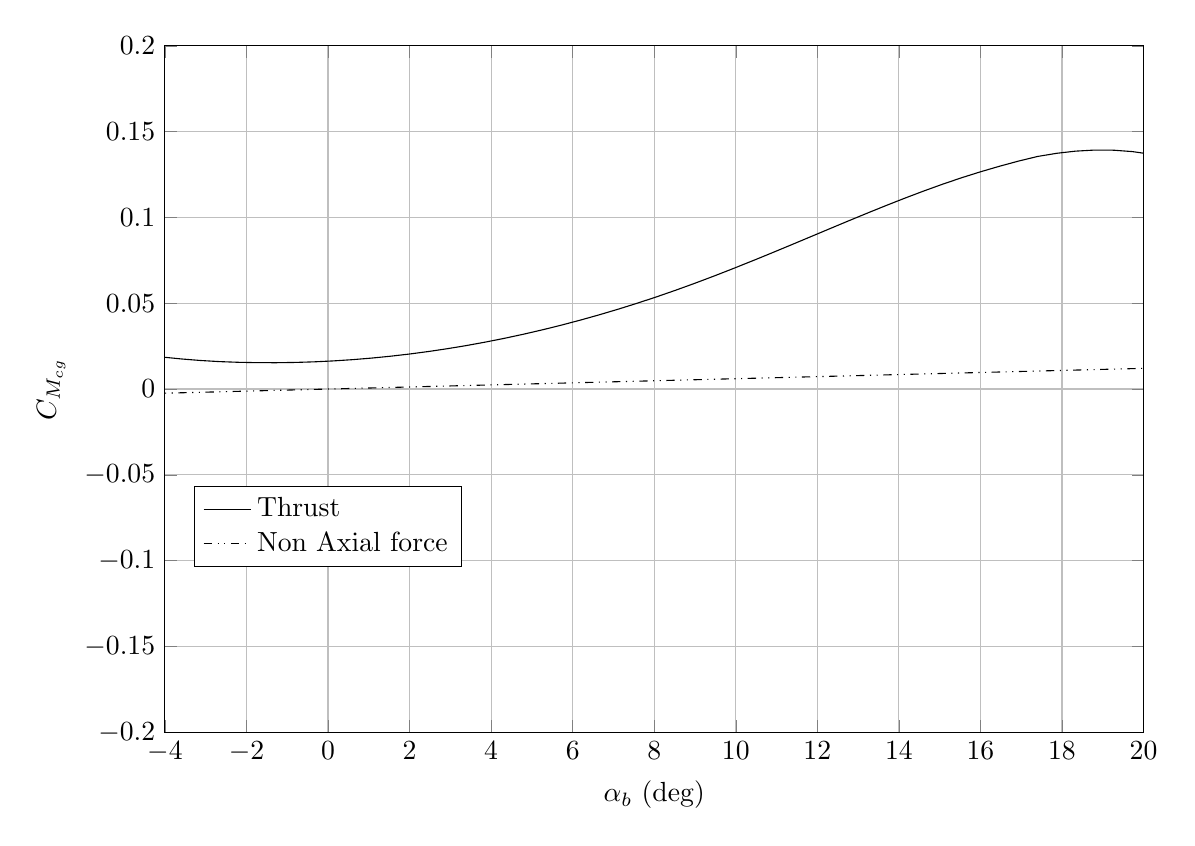
\begin{tikzpicture}

\begin{axis}[
width=14.01cm,
height=10.3cm,
scaled ticks=false, tick label style={/pgf/number format/fixed},
xmin=-4,
xmax=20,
xlabel={$\alpha_{b}$ (deg)},
xmajorgrids,
ymin=-0.2,
ymax=0.2,
ylabel={$C_{M_{cg}}$},
ymajorgrids,
legend style={at={(0.03,0.3)},anchor=west,draw=black,fill=white,legend cell align=left},
legend entries = {Thrust \\ Non Axial force\\}
]

\addplot [
color=black,
solid
]
table[row sep=crcr]{
-4.999999999999999	0.021570650822018575\\
-4.533333333333332	0.02000085813112243\\
-4.0666666666666655	0.01865836770621552\\
-3.5999999999999988	0.01754317954729784\\
-3.133333333333332	0.016655293654369397\\
-2.666666666666665	0.015994710027430182\\
-2.1999999999999984	0.01558802739674183\\
-1.7333333333333318	0.015374490889257325\\
-1.2666666666666653	0.015349312614196082\\
-0.7999999999999987	0.015512111279939688\\
-0.33333333333333215	0.015862503788633207\\
0.13333333333333441	0.016400091428762382\\
0.600000000000001	0.017124485122131633\\
1.0666666666666675	0.018035301111729008\\
1.533333333333334	0.019132149819020255\\
2.000000000000001	0.020414640307694288\\
2.4666666666666677	0.021882380378802795\\
2.9333333333333345	0.02353495917733285\\
3.4000000000000012	0.02537195211664482\\
3.866666666666668	0.02739299892408932\\
4.333333333333335	0.029597703306433933\\
4.800000000000002	0.031985668232490064\\
5.266666666666668	0.034556496041477015\\
5.733333333333335	0.037309788553168174\\
6.200000000000002	0.040245054004529886\\
6.666666666666669	0.04336196691712855\\
7.1333333333333355	0.046660135440486104\\
7.600000000000002	0.05013916049156789\\
8.066666666666668	0.05380025812934947\\
8.533333333333335	0.05764730226375402\\
9.000000000000002	0.061668710038886146\\
9.466666666666669	0.06584924845051271\\
9.933333333333335	0.07016999185035566\\
10.400000000000002	0.07460940790244441\\
10.866666666666669	0.07914357608206717\\
11.333333333333336	0.08374629902113512\\
11.800000000000002	0.08838951870393907\\
12.26666666666667	0.0930445903785934\\
12.733333333333336	0.09767848526601111\\
13.200000000000003	0.1022575783643235\\
13.66666666666667	0.10674687405443531\\
14.133333333333336	0.11111025551761636\\
14.600000000000003	0.11531075585211142\\
15.06666666666667	0.11931450565190461\\
15.533333333333337	0.12308230128084671\\
16.000000000000004	0.12657571431718476\\
16.46666666666667	0.1298175489827388\\
16.933333333333334	0.1328212381998705\\
17.4	0.13551709013128246\\
17.866666666666664	0.1373612142352387\\
18.33333333333333	0.1386250962400392\\
18.799999999999994	0.1392475838403341\\
19.26666666666666	0.13917180946090257\\
19.733333333333324	0.13834660241499672\\
20.19999999999999	0.13672801015634486\\
20.666666666666654	0.13428092862481694\\
21.13333333333332	0.13098084168575044\\
21.599999999999984	0.12681566966293698\\
22.06666666666665	0.12178772696526956\\
22.533333333333314	0.11591578880705147\\
22.999999999999993	0.10923726702196387\\
};

\addplot [
color=black,
dashdotdotted
]
table[row sep=crcr]{
-4.999999999999999	-0.003015548189021825\\
-4.533333333333332	-0.002734097024713121\\
-4.0666666666666655	-0.0024526458604044172\\
-3.5999999999999988	-0.0021711946960957136\\
-3.133333333333332	-0.0018897435317870095\\
-2.666666666666665	-0.001608292367478306\\
-2.1999999999999984	-0.001326841203169602\\
-1.7333333333333318	-0.0010453900388608984\\
-1.2666666666666653	-7.639388745521949E-4\\
-0.7999999999999987	-4.824877102434913E-4\\
-0.33333333333333215	-2.0103654593478764E-4\\
0.13333333333333441	8.0414618373916E-5\\
0.600000000000001	3.618657826826196E-4\\
1.0666666666666675	6.433169469913233E-4\\
1.533333333333334	9.247681113000269E-4\\
2.000000000000001	0.0012062192756087306\\
2.4666666666666677	0.0014876704399174343\\
2.9333333333333345	0.0017691216042261381\\
3.4000000000000012	0.0020505727685348417\\
3.866666666666668	0.002332023932843546\\
4.333333333333335	0.0026134750971522494\\
4.800000000000002	0.002894926261460953\\
5.266666666666668	0.003176377425769657\\
5.733333333333335	0.0034578285900783608\\
6.200000000000002	0.0037392797543870644\\
6.666666666666669	0.004020730918695769\\
7.1333333333333355	0.004302182083004472\\
7.600000000000002	0.004583633247313176\\
8.066666666666668	0.004865084411621879\\
8.533333333333335	0.005146535575930583\\
9.000000000000002	0.005427986740239287\\
9.466666666666669	0.00570943790454799\\
9.933333333333335	0.005990889068856695\\
10.400000000000002	0.006272340233165398\\
10.866666666666669	0.006553791397474101\\
11.333333333333336	0.006835242561782805\\
11.800000000000002	0.007116693726091509\\
12.26666666666667	0.007398144890400213\\
12.733333333333336	0.0076795960547089166\\
13.200000000000003	0.00796104721901762\\
13.66666666666667	0.008242498383326325\\
14.133333333333336	0.008523949547635029\\
14.600000000000003	0.008805400711943731\\
15.06666666666667	0.009086851876252437\\
15.533333333333337	0.00936830304056114\\
16.000000000000004	0.009649754204869843\\
16.46666666666667	0.009931205369178546\\
16.933333333333334	0.010212656533487248\\
17.4	0.01049410769779595\\
17.866666666666664	0.010775558862104653\\
18.33333333333333	0.011057010026413358\\
18.799999999999994	0.01133846119072206\\
19.26666666666666	0.011619912355030763\\
19.733333333333324	0.011901363519339465\\
20.19999999999999	0.012182814683648168\\
20.666666666666654	0.01246426584795687\\
21.13333333333332	0.012745717012265572\\
21.599999999999984	0.013027168176574275\\
22.06666666666665	0.013308619340882979\\
22.533333333333314	0.013590070505191681\\
22.999999999999993	0.013871521669500392\\
};
\end{axis}
\end{tikzpicture}%
\caption{ATR 72 . Mach 0.45. $CM_{cg}$ vs $\alpha_b$. Power effects.}
\label{fig:stallATR}
\end{figure}
\begin{figure}[H]
\centering
%Comparison of CD estimation
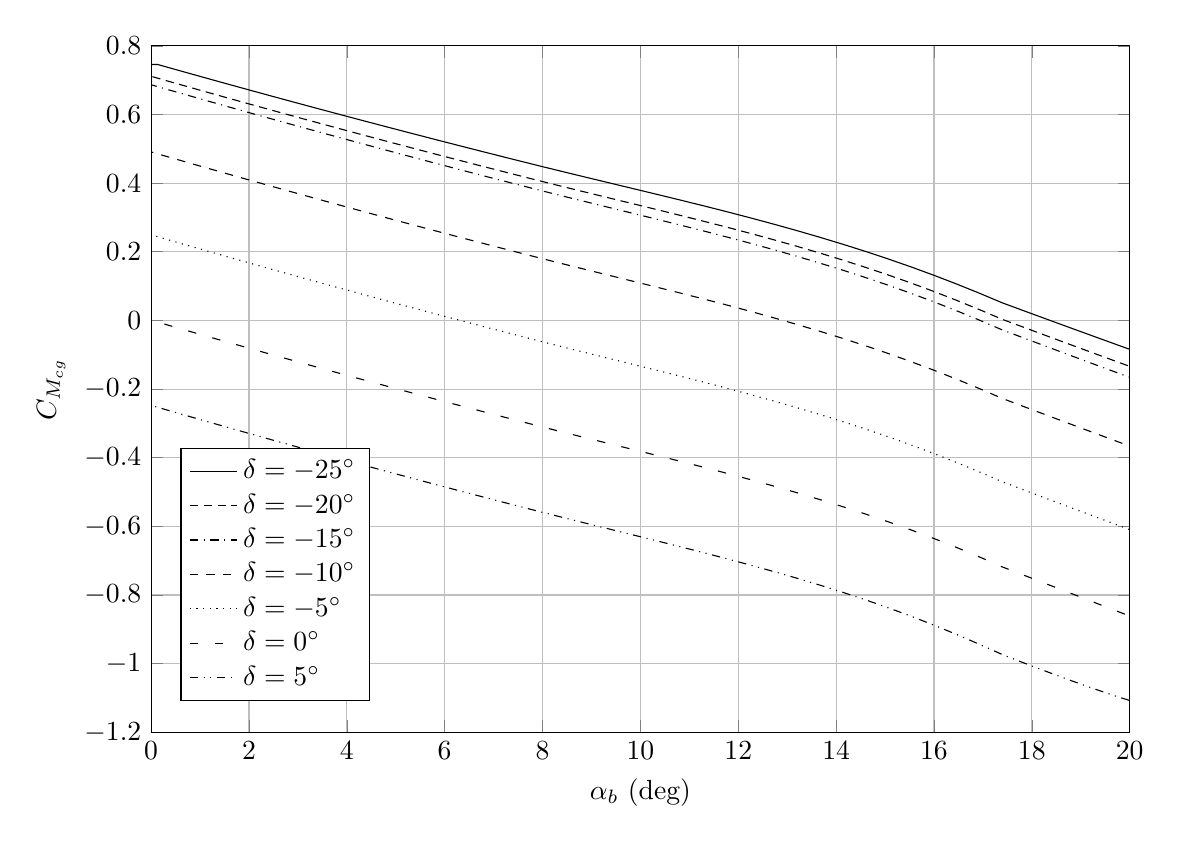
\begin{tikzpicture}

\begin{axis}[
width=14.01cm,
height=10.3cm,
scaled ticks=false, tick label style={/pgf/number format/fixed},
xmin=0,
xmax=20,
xlabel={$\alpha_{b}$ (deg)},
xmajorgrids,
ymin=-1.2,
ymax=0.8,
ylabel={$C_{M_{cg}}$},
ymajorgrids,
legend style={at={(0.03,0.23)},anchor=west,draw=black,fill=white,legend cell align=left},
legend entries = {$\delta = -25^{\circ}$\\$\delta = -20^{\circ}$\\$\delta = -15^{\circ}$\\$\delta = -10^{\circ}$\\$\delta = -5^{\circ}$\\$\delta = 0^{\circ}$\\$\delta = 5^{\circ}$\\}
]

\addplot [
color=black,
solid
]
table[row sep=crcr]{
-4.999999999999999	0.6524318987565378\\
-4.533333333333332	0.6611449328105656\\
-4.0666666666666655	0.6699771616040189\\
-3.5999999999999988	0.6789348202357504\\
-3.133333333333332	0.6880123525605751\\
-2.666666666666665	0.6972150810334512\\
-2.1999999999999984	0.7065698458263154\\
-1.7333333333333318	0.7160138324562046\\
-1.2666666666666653	0.7255380969649831\\
-0.7999999999999987	0.7351454222895258\\
-0.33333333333333215	0.7448331934666084\\
0.13333333333333441	0.7456402003925402\\
0.600000000000001	0.7269129537818834\\
1.0666666666666675	0.7083209282288025\\
1.533333333333334	0.689862974292562\\
2.000000000000001	0.6715404134575506\\
2.4666666666666677	0.6533524409329499\\
2.9333333333333345	0.6352991382824793\\
3.4000000000000012	0.6173819420707719\\
3.866666666666668	0.5995982557112967\\
4.333333333333335	0.5819498684396486\\
4.800000000000002	0.5644339664048602\\
5.266666666666668	0.5470525890443363\\
5.733333333333335	0.5298029025241102\\
6.200000000000002	0.5126913110451266\\
6.666666666666669	0.49571082653612614\\
7.1333333333333355	0.47886493625206006\\
7.600000000000002	0.4621492692501782\\
8.066666666666668	0.44558207996447324\\
8.533333333333335	0.4292820535030928\\
9.000000000000002	0.4131768125506479\\
9.466666666666669	0.39715772316256553\\
9.933333333333335	0.38115095646586683\\
10.400000000000002	0.36507062463317125\\
10.866666666666669	0.34883559575217954\\
11.333333333333336	0.3323244689657924\\
11.800000000000002	0.3154288105496084\\
12.26666666666667	0.29804479633358033\\
12.733333333333336	0.2801002505172361\\
13.200000000000003	0.2615122621512705\\
13.66666666666667	0.24219202894491468\\
14.133333333333336	0.22205489183108876\\
14.600000000000003	0.20101055726072048\\
15.06666666666667	0.17892969756221042\\
15.533333333333337	0.15574077187130306\\
16.000000000000004	0.13136502182606472\\
16.46666666666667	0.10577189852013474\\
16.933333333333334	0.07892115856281848\\
17.4	0.050960448486813206\\
17.866666666666664	0.026460470297814006\\
18.33333333333333	0.0020477867071489273\\
18.799999999999994	-0.022274589750000972\\
19.26666666666666	-0.046490438853045685\\
19.733333333333324	-0.07058372781914293\\
20.19999999999999	-0.0945198622805352\\
20.666666666666654	-0.1182641942397318\\
21.13333333333332	-0.14175735586281954\\
21.599999999999984	-0.1649374101990993\\
22.06666666666665	-0.18771047245442127\\
22.533333333333314	-0.20998114792036524\\
22.999999999999993	0.0\\
};

\addplot [
color=black,
densely dashed
]
table[row sep=crcr]{
-4.999999999999999	0.6550078359667001\\
-4.533333333333332	0.6637208700207279\\
-4.0666666666666655	0.672553098814181\\
-3.5999999999999988	0.6815107574459124\\
-3.133333333333332	0.6905882897707373\\
-2.666666666666665	0.6997910182436132\\
-2.1999999999999984	0.7091457830364776\\
-1.7333333333333318	0.7185897696663666\\
-1.2666666666666653	0.7281140341751452\\
-0.7999999999999987	0.737721359499688\\
-0.33333333333333215	0.7248062324115125\\
0.13333333333333441	0.7057320974892591\\
0.600000000000001	0.6867930916996277\\
1.0666666666666675	0.6679897084209598\\
1.533333333333334	0.6493207995808427\\
2.000000000000001	0.630787687976801\\
2.4666666666666677	0.612389570074601\\
2.9333333333333345	0.5941265344508224\\
3.4000000000000012	0.5760000261931869\\
3.866666666666668	0.5580074366977206\\
4.333333333333335	0.5401505562065281\\
4.800000000000002	0.5224265718119737\\
5.266666666666668	0.5048375238304679\\
5.733333333333335	0.48738057924161987\\
6.200000000000002	0.4700621607624285\\
6.666666666666669	0.4528752647524136\\
7.1333333333333355	0.4358233776066126\\
7.600000000000002	0.41890212891179907\\
8.066666666666668	0.40212985818158864\\
8.533333333333335	0.385626293458737\\
9.000000000000002	0.3693187286166405\\
9.466666666666669	0.35309772765626724\\
9.933333333333335	0.33688883065487807\\
10.400000000000002	0.3206055280593048\\
10.866666666666669	0.3041660562101582\\
11.333333333333336	0.28744837221254216\\
11.800000000000002	0.2703433583345017\\
12.26666666666667	0.2527463482846131\\
12.733333333333336	0.23458460346210996\\
13.200000000000003	0.21577452213336304\\
13.66666666666667	0.19622659760558434\\
14.133333333333336	0.175855451780457\\
14.600000000000003	0.15457005631293358\\
15.06666666666667	0.13223999051403398\\
15.533333333333337	0.10879309276373031\\
16.000000000000004	0.08414989397688778\\
16.46666666666667	0.05827902880556268\\
16.933333333333334	0.031139413537651463\\
17.4	0.0028798489060172395\\
17.866666666666664	-0.021891374371809328\\
18.33333333333333	-0.04657530305130183\\
18.799999999999994	-0.07116892459727876\\
19.26666666666666	-0.09565601878915084\\
19.733333333333324	-0.12002055284407578\\
20.19999999999999	-0.14422793239429518\\
20.666666666666654	-0.16824350944231883\\
21.13333333333332	-0.19200791615423404\\
21.599999999999984	-0.21545921557934117\\
22.06666666666665	-0.2385035229234906\\
22.533333333333314	-0.26104544347826175\\
22.999999999999993	0.0\\
};

\addplot [
color=black,
dashdotted
]
table[row sep=crcr]{
-4.999999999999999	0.6564072169665783\\
-4.533333333333332	0.6651202510206061\\
-4.0666666666666655	0.6739524798140593\\
-3.5999999999999988	0.6829101384457907\\
-3.133333333333332	0.6919876707706156\\
-2.666666666666665	0.7011903992434916\\
-2.1999999999999984	0.7105451640363558\\
-1.7333333333333318	0.719989150666245\\
-1.2666666666666653	0.7295134151750234\\
-0.7999999999999987	0.7196355579591093\\
-0.33333333333333215	0.7002624480887095\\
0.13333333333333441	0.6810284052643376\\
0.600000000000001	0.6619297973987707\\
1.0666666666666675	0.6429671146180362\\
1.533333333333334	0.624139209881021\\
2.000000000000001	0.6054474069749547\\
2.4666666666666677	0.586890903312688\\
2.9333333333333345	0.5684697927563647\\
3.4000000000000012	0.5501855268175264\\
3.866666666666668	0.5320354878346983\\
4.333333333333335	0.5140214668085886\\
4.800000000000002	0.49614065154254616\\
5.266666666666668	0.47839508301548445\\
5.733333333333335	0.46078192882020225\\
6.200000000000002	0.4433076256291771\\
6.666666666666669	0.4259651580674664\\
7.1333333333333355	0.4087580118819947\\
7.600000000000002	0.3916818170586348\\
8.066666666666668	0.37475497723518625\\
8.533333333333335	0.35809800651019374\\
9.000000000000002	0.3416379509333102\\
9.466666666666669	0.32526477000015336\\
9.933333333333335	0.30890352816821526\\
10.400000000000002	0.29246724729200096\\
10.866666666666669	0.27587368756677766\\
11.333333333333336	0.2590003221962398\\
11.800000000000002	0.24173751791457868\\
12.26666666666667	0.22397997372674\\
12.733333333333336	0.2056545268515467\\
13.200000000000003	0.18667705491389103\\
13.66666666666667	0.1669575203159016\\
14.133333333333336	0.14641000302819338\\
14.600000000000003	0.12494292089282803\\
15.06666666666667	0.10242502941784402\\
15.533333333333337	0.07878369912198355\\
16.000000000000004	0.05393892525077844\\
16.46666666666667	0.027858727107414605\\
16.933333333333334	5.013876327853786E-4\\
17.4	-0.027983422524035392\\
17.866666666666664	-0.052959082178475\\
18.33333333333333	-0.07784744723458066\\
18.799999999999994	-0.1026455051571711\\
19.26666666666666	-0.12733703572565622\\
19.733333333333324	-0.15190600615719432\\
20.19999999999999	-0.1763178220840271\\
20.666666666666654	-0.20053783550866403\\
21.13333333333332	-0.22450667859719228\\
21.599999999999984	-0.24816241439891257\\
22.06666666666665	-0.2714111581196752\\
22.533333333333314	-0.2941575150510597\\
22.999999999999993	0.0\\
};

\addplot [
color=black,
dashed
]
table[row sep=crcr]{
-4.999999999999999	0.6564988915450297\\
-4.533333333333332	0.6652119255990575\\
-4.0666666666666655	0.6740441543925106\\
-3.5999999999999988	0.6601375378719498\\
-3.133333333333332	0.6320078047131106\\
-2.666666666666665	0.6040032677023227\\
-2.1999999999999984	0.5832713530240214\\
-1.7333333333333318	0.563393155113534\\
-1.2666666666666653	0.543649233444402\\
-0.7999999999999987	0.5240425946336517\\
-0.33333333333333215	0.5045708408651114\\
0.13333333333333441	0.4852383449656518\\
0.600000000000001	0.466041472317932\\
1.0666666666666675	0.44698071104557446\\
1.533333333333334	0.42805491474242297\\
2.000000000000001	0.409265407805055\\
2.4666666666666677	0.3906113882294273\\
2.9333333333333345	0.3720929531319329\\
3.4000000000000012	0.35371155797917\\
3.866666666666668	0.3354645795330861\\
4.333333333333335	0.31735380926145096\\
4.800000000000002	0.29937643540535663\\
5.266666666666668	0.2815344993516112\\
5.733333333333335	0.263825169070545\\
6.200000000000002	0.2462548898268302\\
6.666666666666669	0.22881663902077884\\
7.1333333333333355	0.2115139020002812\\
7.600000000000002	0.19434230899693014\\
8.066666666666668	0.17732030312889477\\
8.533333333333335	0.16056888245835502\\
9.000000000000002	0.14401494045332566\\
9.466666666666669	0.127548064423874\\
9.933333333333335	0.11109302599500384\\
10.400000000000002	0.09456255851543097\\
10.866666666666669	0.07787412902434551\\
11.333333333333336	0.060904912794062877\\
11.800000000000002	0.043544959151738845\\
12.26666666666667	0.025688576324105795\\
12.733333333333336	0.00726234036799789\\
13.200000000000003	-0.011818191643422337\\
13.66666666666667	-0.031643384178914664\\
14.133333333333336	-0.052299490927298374\\
14.600000000000003	-0.0738784350214194\\
15.06666666666667	-0.0965119681572967\\
15.533333333333337	-0.1202730078718511\\
16.000000000000004	-0.14524188872372204\\
16.46666666666667	-0.17145097027147976\\
16.933333333333334	-0.19894235951718606\\
17.4	-0.2275658502164349\\
17.866666666666664	-0.2526673785094517\\
18.33333333333333	-0.27768161220413423\\
18.799999999999994	-0.3026055387653014\\
19.26666666666666	-0.32742293797236377\\
19.733333333333324	-0.3521177770424787\\
20.19999999999999	-0.3766554616078886\\
20.666666666666654	-0.40100134367110285\\
21.13333333333332	-0.42509605539820794\\
21.599999999999984	-0.44887765983850497\\
22.06666666666665	-0.47225459161398065\\
22.533333333333314	-0.49515620732671284\\
22.999999999999993	0.0\\
};

\addplot [
color=black,
dotted
]
table[row sep=crcr]{
-4.999999999999999	0.504173358604879\\
-4.533333333333332	0.47563617945024234\\
-4.0666666666666655	0.4472181950350311\\
-3.5999999999999988	0.41892564045809816\\
-3.133333333333332	0.3907529595742587\\
-2.666666666666665	0.3627054748384703\\
-2.1999999999999984	0.3419388316086533\\
-1.7333333333333318	0.3220267875903781\\
-1.2666666666666653	0.3022490821428661\\
-0.7999999999999987	0.28260872214133376\\
-0.33333333333333215	0.26310331002025855\\
0.13333333333333441	0.24373722087912966\\
0.600000000000001	0.22450681923730254\\
1.0666666666666675	0.20541259253515792\\
1.533333333333334	0.18645339458319374\\
2.000000000000001	0.16763054998590335\\
2.4666666666666677	0.1489432569382057\\
2.9333333333333345	0.1303916136668781\\
3.4000000000000012	0.11197707698802643\\
3.866666666666668	0.0936970217608107\\
4.333333333333335	0.07555323961236636\\
4.800000000000002	0.05754291893314874\\
5.266666666666668	0.03966810124914345\\
5.733333333333335	0.021925954659499012\\
6.200000000000002	0.0043229273606361154\\
6.666666666666669	-0.013148005712293586\\
7.1333333333333355	-0.030483359347554626\\
7.600000000000002	-0.04768750322971176\\
8.066666666666668	-0.06474198076947173\\
8.533333333333335	-0.08152562877108879\\
9.000000000000002	-0.09811160582903401\\
9.466666666666669	-0.11461045162692883\\
9.933333333333335	-0.13109749445734462\\
10.400000000000002	-0.14766009941282496\\
10.866666666666669	-0.1643808994821668\\
11.333333333333336	-0.18138282105042652\\
11.800000000000002	-0.19877592309312184\\
12.26666666666667	-0.21666603072122356\\
12.733333333333336	-0.23512665698916066\\
13.200000000000003	-0.254242354199447\\
13.66666666666667	-0.2741035983526838\\
14.133333333333336	-0.29479675698585606\\
14.600000000000003	-0.31641386957609297\\
15.06666666666667	-0.33908686088286005\\
15.533333333333337	-0.36288874673074967\\
16.000000000000004	-0.38789997421110994\\
16.46666666666667	-0.4141530321541918\\
16.933333333333334	-0.44169016061476263\\
17.4	-0.4703609705975637\\
17.866666666666664	-0.49550544661558077\\
18.33333333333333	-0.520562628035264\\
18.799999999999994	-0.5455295023214315\\
19.26666666666666	-0.5703975324156825\\
19.733333333333324	-0.5952093308312724\\
20.19999999999999	-0.6199722806721916\\
20.666666666666654	-0.644682919652139\\
21.13333333333332	-0.6693176918555954\\
21.599999999999984	-0.6938034029718937\\
22.06666666666665	-0.7179532720832182\\
22.533333333333314	-0.7416047850289127\\
22.999999999999993	0.0\\
};

\addplot [
color=black,
loosely dashed
]
table[row sep=crcr]{
-4.999999999999999	0.25506382852105397\\
-4.533333333333332	0.22656761473870604\\
-4.0666666666666655	0.1981905956957833\\
-3.5999999999999988	0.169939006491139\\
-3.133333333333332	0.14180729097958808\\
-2.666666666666665	0.11380077161608824\\
-2.1999999999999984	0.09306725396025381\\
-1.7333333333333318	0.07318749380348784\\
-1.2666666666666653	0.053442012765036725\\
-0.7999999999999987	0.03383381747384451\\
-0.33333333333333215	0.014360510125308519\\
0.13333333333333441	-0.004973536348802539\\
0.600000000000001	-0.024171956605677305\\
1.0666666666666675	-0.0432342625532299\\
1.533333333333334	-0.06216160058761635\\
2.000000000000001	-0.08095264630266241\\
2.4666666666666677	-0.09960820169322754\\
2.9333333333333345	-0.11812816959166669\\
3.4000000000000012	-0.13651109446909182\\
3.866666666666668	-0.15475959965138275\\
4.333333333333335	-0.17287189366341435\\
4.800000000000002	-0.19085078825719995\\
5.266666666666668	-0.20869424203950765\\
5.733333333333335	-0.2264050870340611\\
6.200000000000002	-0.24397687784086633\\
6.666666666666669	-0.26141663717339664\\
7.1333333333333355	-0.27872087969004633\\
7.600000000000002	-0.29589397515535254\\
8.066666666666668	-0.31291747982935497\\
8.533333333333335	-0.3296703880277476\\
9.000000000000002	-0.3462258086855814\\
9.466666666666669	-0.36269416035448016\\
9.933333333333335	-0.3791506760213691\\
10.400000000000002	-0.39568262688131933\\
10.866666666666669	-0.41237255051216637\\
11.333333333333336	-0.4293432763338287\\
11.800000000000002	-0.44670476001811327\\
12.26666666666667	-0.4645626994928018\\
12.733333333333336	-0.48299052281419885\\
13.200000000000003	-0.5020726779576322\\
13.66666666666667	-0.5218995345398744\\
14.133333333333336	-0.5425573515046734\\
14.600000000000003	-0.5641380573550173\\
15.06666666666667	-0.5867734117750736\\
15.533333333333337	-0.6105363420411448\\
16.000000000000004	-0.6355072026189118\\
16.46666666666667	-0.6617503444982138\\
16.933333333333334	-0.6893864863442695\\
17.4	-0.7183338265560615\\
17.866666666666664	-0.7439062084787781\\
18.33333333333333	-0.76957343468621\\
18.799999999999994	-0.7953416068382508\\
19.26666666666666	-0.8210742296158242\\
19.733333333333324	-0.8466859635617349\\
20.19999999999999	-0.8720638282732395\\
20.666666666666654	-0.8969877580953883\\
21.13333333333332	-0.9211766237884585\\
21.599999999999984	-0.9444455385625764\\
22.06666666666665	-0.9665345561046943\\
22.533333333333314	-0.9871404976154075\\
22.999999999999993	0.0\\
};

\addplot [
color=black,
dashdotdotted
]
table[row sep=crcr]{
-4.999999999999999	0.007292222645310203\\
-4.533333333333332	-0.02124495650932635\\
-4.0666666666666655	-0.04966294092453762\\
-3.5999999999999988	-0.07795549550147055\\
-3.133333333333332	-0.10612817638531008\\
-2.666666666666665	-0.1341756611210985\\
-2.1999999999999984	-0.15494230435091536\\
-1.7333333333333318	-0.17485434836919056\\
-1.2666666666666653	-0.19463205381670273\\
-0.7999999999999987	-0.21427241381823506\\
-0.33333333333333215	-0.23377782593931015\\
0.13333333333333441	-0.25314391508043904\\
0.600000000000001	-0.2723743167222662\\
1.0666666666666675	-0.2914685434244108\\
1.533333333333334	-0.31042774137637497\\
2.000000000000001	-0.32925058597366547\\
2.4666666666666677	-0.3479378790213631\\
2.9333333333333345	-0.36648952229269066\\
3.4000000000000012	-0.38490405897154234\\
3.866666666666668	-0.4031841141987581\\
4.333333333333335	-0.4213278963472024\\
4.800000000000002	-0.43933821702642006\\
5.266666666666668	-0.45721303471042535\\
5.733333333333335	-0.4749551813000698\\
6.200000000000002	-0.4925582085989328\\
6.666666666666669	-0.5100291416718624\\
7.1333333333333355	-0.5273644953071234\\
7.600000000000002	-0.5445686391892806\\
8.066666666666668	-0.5616231167290403\\
8.533333333333335	-0.5784067647306576\\
9.000000000000002	-0.5949927417886027\\
9.466666666666669	-0.6114915875864978\\
9.933333333333335	-0.6279786304169133\\
10.400000000000002	-0.6445412353723936\\
10.866666666666669	-0.6612620354417357\\
11.333333333333336	-0.6782639570099953\\
11.800000000000002	-0.6956570590526906\\
12.26666666666667	-0.7135480635392617\\
12.733333333333336	-0.7320109757622953\\
13.200000000000003	-0.7511779531467554\\
13.66666666666667	-0.7711412760600492\\
14.133333333333336	-0.7920712382652088\\
14.600000000000003	-0.8140970168967737\\
15.06666666666667	-0.8373284389166005\\
15.533333333333337	-0.8618888470974716\\
16.000000000000004	-0.8878758055484575\\
16.46666666666667	-0.9152224347111271\\
16.933333333333334	-0.9439081805088175\\
17.4	-0.9736550254067224\\
17.866666666666664	-0.9995279993453591\\
18.33333333333333	-1.02477643903381\\
18.799999999999994	-1.0493049144140658\\
19.26666666666666	-1.0729368240812045\\
19.733333333333324	-1.095489183719595\\
20.19999999999999	-1.1161023156156167\\
20.666666666666654	-1.1348366784643773\\
21.13333333333332	-1.1514257041390505\\
21.599999999999984	-1.1655619173793457\\
22.06666666666665	-1.1761868288031836\\
22.533333333333314	-1.182756005657917\\
22.999999999999993	0.0\\
};
\end{axis}
\end{tikzpicture}%

\caption{ATR 72 . Mach 0.45. Aircraft $CM_{cg}$ vs $\alpha_b$ with elevator deflections.}
\label{fig:stallATR}
\end{figure}
\noindent\\
\begin{figure}[H]
\centering
%Comparison of CD estimation
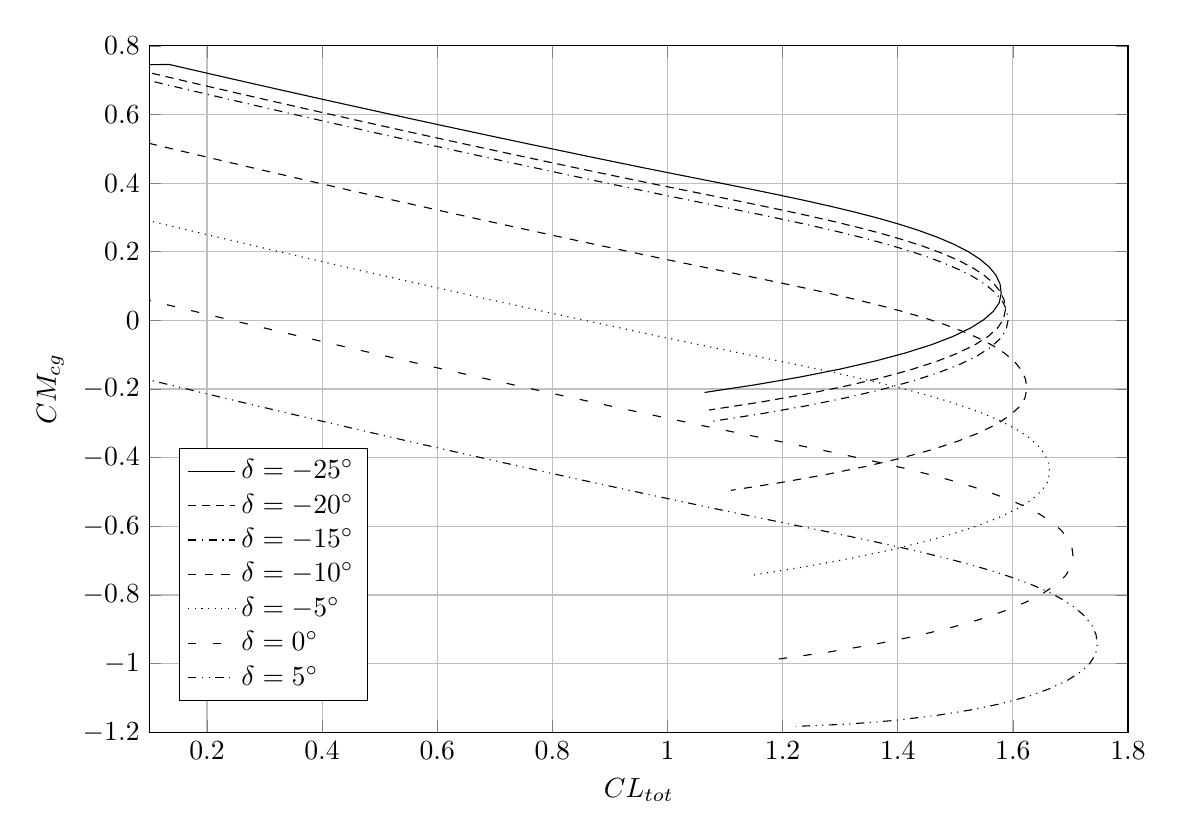
\begin{tikzpicture}

\begin{axis}[
width=14.01cm,
height=10.3cm,
scaled ticks=false, tick label style={/pgf/number format/fixed},
xmin=0.1,
xmax=1.8,
xlabel={$CL_{tot}$},
xmajorgrids,
ymin=-1.2,
ymax=0.8,
ylabel={$CM_{cg}$},
ymajorgrids,
legend style={at={(0.03,0.23)},anchor=west,draw=black,fill=white,legend cell align=left},
legend entries = {$\delta = -25^{\circ}$\\$\delta = -20^{\circ}$\\$\delta = -15^{\circ}$\\$\delta = -10^{\circ}$\\$\delta = -5^{\circ}$\\$\delta = 0^{\circ}$\\$\delta = 5^{\circ}$\\}
]

\addplot [
color=black,
solid
]
table[row sep=crcr]{
-0.3471334642807813	0.6524318987565378\\
-0.30348056228561016	0.6611449328105656\\
-0.25982766029043897	0.6699771616040189\\
-0.2161747582952678	0.6789348202357504\\
-0.17252185630009662	0.6880123525605751\\
-0.12886895430492545	0.6972150810334512\\
-0.08521605230975428	0.7065698458263154\\
-0.0415631503145831	0.7160138324562046\\
0.002089751680588031	0.7255380969649831\\
0.04574265367575919	0.7351454222895258\\
0.08939555567093033	0.7448331934666084\\
0.13452894861538855	0.7456402003925402\\
0.18290195785697744	0.7269129537818834\\
0.23126601871175664	0.7083209282288025\\
0.2796211006798399	0.689862974292562\\
0.32796717449147245	0.6715404134575506\\
0.3763042121373785	0.6533524409329499\\
0.4246320573011014	0.6352991382824793\\
0.47295052000316445	0.6173819420707719\\
0.5212598681121062	0.5995982557112967\\
0.5695600791928366	0.5819498684396486\\
0.6178511322185285	0.5644339664048602\\
0.666133007596158	0.5470525890443363\\
0.7144056871911388	0.5298029025241102\\
0.7626687582810414	0.5126913110451266\\
0.8109225679034555	0.49571082653612614\\
0.8591671352258254	0.47886493625206006\\
0.9074024484450889	0.4621492692501782\\
0.9556657862020534	0.44558207996447324\\
1.0041263356051073	0.4292820535030928\\
1.0525552202017912	0.4131768125506479\\
1.1006543008615628	0.39715772316256553\\
1.1481216267630743	0.38115095646586683\\
1.194655039253836	0.36507062463317125\\
1.2399526030559629	0.34883559575217954\\
1.2837126122711813	0.3323244689657924\\
1.3256342965061445	0.3154288105496084\\
1.365420409720979	0.29804479633358033\\
1.4027674798153131	0.2801002505172361\\
1.4373748874498455	0.2615122621512705\\
1.4689423168233948	0.24219202894491468\\
1.4971697782197084	0.22205489183108876\\
1.5217576333181908	0.20101055726072048\\
1.5424142285451603	0.17892969756221042\\
1.5588373836265126	0.15574077187130306\\
1.5707269236600594	0.13136502182606472\\
1.5777850302039367	0.10577189852013474\\
1.579714417097048	0.07892115856281848\\
1.576173340338095	0.050960448486813206\\
1.5660079314956457	0.026460470297814006\\
1.5495175880459309	0.0020477867071489273\\
1.5263862930829049	-0.022274589750000972\\
1.49629802970052	-0.046490438853045685\\
1.4589367809927312	-0.07058372781914293\\
1.4139865300534933	-0.0945198622805352\\
1.3611312599767575	-0.1182641942397318\\
1.3000549538564796	-0.14175735586281954\\
1.2304415947866125	-0.1649374101990993\\
1.15197516586111	-0.18771047245442127\\
1.0643396501739297	-0.20998114792036524\\
};

\addplot [
color=black,
densely dashed
]
table[row sep=crcr]{
-0.34809347859707673	0.6550078359667001\\
-0.3044405766019056	0.6637208700207279\\
-0.26078767460673435	0.672553098814181\\
-0.21713477261156322	0.6815107574459124\\
-0.17348187061639203	0.6905882897707373\\
-0.12982896862122087	0.6997910182436132\\
-0.0861760666260497	0.7091457830364776\\
-0.04252316463087852	0.7185897696663666\\
0.0011297373642926156	0.7281140341751452\\
0.04478263935946378	0.737721359499688\\
0.09216878846158646	0.7248062324115125\\
0.14058588486816725	0.7057320974892591\\
0.18899386968381748	0.6867930916996277\\
0.2373928398059092	0.6679897084209598\\
0.28578276450855467	0.6493207995808427\\
0.33416361430511293	0.630787687976801\\
0.38253536097876195	0.612389570074601\\
0.43089784705475404	0.5941265344508224\\
0.4792508811458815	0.5760000261931869\\
0.5275947331055648	0.5580074366977206\\
0.575929380332472	0.5401505562065281\\
0.6242548016439691	0.5224265718119737\\
0.6725709773018494	0.5048375238304679\\
0.7208778890371511	0.48738057924161987\\
0.7691751210692083	0.4700621607624285\\
0.8174630230071281	0.4528752647524136\\
0.8657416141603842	0.4358233776066126\\
0.9140108826384543	0.41890212891179907\\
0.962308093029822	0.40212985818158864\\
1.0108022601847622	0.385626293458737\\
1.059264561959493	0.3693187286166405\\
1.1073969916961959	0.35309772765626724\\
1.1548977028019565	0.33688883065487807\\
1.2014646393127097	0.3206055280593048\\
1.24679597029418	0.3041660562101582\\
1.2905900958913858	0.28744837221254216\\
1.332546358686281	0.2703433583345017\\
1.3723676517294374	0.2527463482846131\\
1.4097505958763759	0.23458460346210996\\
1.444394685882392	0.21577452213336304\\
1.4759997222900927	0.19622659760558434\\
1.504265834143273	0.175855451780457\\
1.5288935044851966	0.15457005631293358\\
1.5495912602723028	0.13223999051403398\\
1.5660570237586975	0.10879309276373031\\
1.5779907374300286	0.08414989397688778\\
1.585094717693431	0.05827902880556268\\
1.5870718171809577	0.031139413537651463\\
1.5835801012558284	0.0028798489060172395\\
1.5734594930814727	-0.021891374371809328\\
1.5570139502998517	-0.04657530305130183\\
1.5339274560049194	-0.07116892459727876\\
1.5038839932906283	-0.09565601878915084\\
1.4665675452509332	-0.12002055284407578\\
1.4216620949797893	-0.14422793239429518\\
1.3688516255711474	-0.16824350944231883\\
1.3078201201189632	-0.19200791615423404\\
1.2382515617171899	-0.21545921557934117\\
1.159829933459781	-0.2385035229234906\\
1.0722392184406948	-0.26104544347826175\\
};

\addplot [
color=black,
dashdotted
]
table[row sep=crcr]{
-0.3488170376822153	0.6564072169665783\\
-0.30516413568704415	0.6651202510206061\\
-0.261511233691873	0.6739524798140593\\
-0.21785833169670182	0.6829101384457907\\
-0.17420542970153063	0.6919876707706156\\
-0.13055252770635947	0.7011903992434916\\
-0.0868996257111883	0.7105451640363558\\
-0.04324672371601712	0.719989150666245\\
4.061782791540125E-4	0.7295134151750234\\
0.04727738442691229	0.7196355579591093\\
0.09573017751670179	0.7002624480887095\\
0.1441736853907836	0.6810284052643376\\
0.19260803116162006	0.6619297973987707\\
0.24103331226375735	0.6429671146180362\\
0.28944949780097134	0.624139209881021\\
0.3378565581231546	0.6054474069749547\\
0.38625446485705844	0.586890903312688\\
0.43464305965493555	0.5684697927563647\\
0.48302215006857696	0.5501855268175264\\
0.531392007447401	0.5320354878346983\\
0.5797526090647798	0.5140214668085886\\
0.6281039336206481	0.49614065154254616\\
0.676445961267376	0.47839508301548445\\
0.7247786736347229	0.46078192882020225\\
0.773101652637042	0.4433076256291771\\
0.8214152498215838	0.4259651580674664\\
0.8697194846048679	0.4087580118819947\\
0.9180143450304548	0.3916818170586348\\
0.966337085095645	0.37475497723518625\\
1.0148565898204385	0.35809800651019374\\
1.0633440779932937	0.3416379509333102\\
1.1115016428005733	0.32526477000015336\\
1.1590275162059307	0.30890352816821526\\
1.2056197196411698	0.29246724729200096\\
1.2509765008153908	0.27587368756677766\\
1.2947963397980327	0.2590003221962398\\
1.336778664320097	0.24173751791457868\\
1.3766264722640877	0.22397997372674\\
1.4140364545460224	0.2056545268515467\\
1.4487081919138551	0.18667705491389103\\
1.480341572598056	0.1669575203159016\\
1.5086368151514105	0.14641000302819338\\
1.5332944940886537	0.12494292089282803\\
1.554023272431081	0.10242502941784402\\
1.5705211497079143	0.07878369912198355\\
1.5824881568795615	0.05393892525077844\\
1.5896267119883254	0.027858727107414605\\
1.5916397722741227	5.013876327853786E-4\\
1.5881852594189443	-0.027983422524035392\\
1.5780984173352284	-0.052959082178475\\
1.5616866406442473	-0.07784744723458066\\
1.5386339124399546	-0.1026455051571711\\
1.5086242158163035	-0.12733703572565622\\
1.4713415338672482	-0.15190600615719432\\
1.426469849686744	-0.1763178220840271\\
1.3736931463687418	-0.20053783550866403\\
1.3126954070071974	-0.22450667859719228\\
1.243160614696064	-0.24816241439891257\\
1.164772752529295	-0.2714111581196752\\
1.0772158036008486	-0.2941575150510597\\
};

\addplot [
color=black,
dashed
]
table[row sep=crcr]{
-0.34926252296465465	0.6564988915450297\\
-0.3056096209694835	0.6652119255990575\\
-0.26195671897431233	0.6740441543925106\\
-0.21452739910285312	0.6601375378719498\\
-0.1647290942219834	0.6320078047131106\\
-0.11493078934111371	0.6040032677023227\\
-0.0663085684658876	0.5832713530240214\\
-0.01781261672903274	0.563393155113534\\
0.030674416274122956	0.543649233444402\\
0.07915249359905727	0.5240425946336517\\
0.12762157938029853	0.5045708408651114\\
0.17608134842820983	0.4852383449656518\\
0.2245319242731449	0.466041472317932\\
0.27297340468038056	0.44698071104557446\\
0.3214057586488189	0.42805491474242297\\
0.3698289564277086	0.409265407805055\\
0.418242969547491	0.3906113882294273\\
0.46664763912292534	0.3720929531319329\\
0.5150427720525587	0.35371155797917\\
0.5634286406068746	0.3354645795330861\\
0.611805221982102	0.31735380926145096\\
0.6601724948058754	0.29937643540535663\\
0.7085304391631938	0.2815344993516112\\
0.7568790366214613	0.263825169070545\\
0.8052178676758861	0.2462548898268302\\
0.8535472850670062	0.22881663902077884\\
0.9018673082772489	0.2115139020002812\\
0.9501779253095894	0.19434230899693014\\
0.9985163836404846	0.17732030312889477\\
1.0470514883552364	0.16056888245835502\\
1.0955544834437156	0.14401494045332566\\
1.1437275235649602	0.127548064423874\\
1.1912688890488128	0.11109302599500384\\
1.2378766489786384	0.09456255851543097\\
1.283249099483172	0.07787412902434551\\
1.3270847698402084	0.060904912794062877\\
1.3690831402058359	0.043544959151738845\\
1.4089472730061234	0.025688576324105795\\
1.4463739022923634	0.00726234036799789\\
1.4810626617569957	-0.011818191643422337\\
1.5127134936186908	-0.031643384178914664\\
1.5410266715396763	-0.052299490927298374\\
1.5657028263524022	-0.0738784350214194\\
1.5864507048514072	-0.0965119681572967\\
1.6029683541431285	-0.1202730078718511\\
1.6149558596606552	-0.14524188872372204\\
1.622115702021653	-0.17145097027147976\\
1.6241509028716465	-0.19894235951718606\\
1.6207192954300895	-0.2275658502164349\\
1.6106532426595543	-0.2526673785094517\\
1.5942622552817536	-0.27768161220413423\\
1.5712303163906416	-0.3026055387653014\\
1.5412414090801707	-0.32742293797236377\\
1.503979516444296	-0.3521177770424787\\
1.4591286215769723	-0.3766554616078886\\
1.4063727075721508	-0.40100134367110285\\
1.345395757523787	-0.42509605539820794\\
1.2758817545258339	-0.44887765983850497\\
1.1975150647626562	-0.47225459161398065\\
1.1099837594215713	-0.49515620732671284\\
};

\addplot [
color=black,
dotted
]
table[row sep=crcr]{
-0.3244319352636276	0.504173358604879\\
-0.27462653684686594	0.47563617945024234\\
-0.2248211384301042	0.4472181950350311\\
-0.17501574001334247	0.41892564045809816\\
-0.12521034159658076	0.3907529595742587\\
-0.07540494317981904	0.3627054748384703\\
-0.026776986302822173	0.3419388316086533\\
0.021724555685446373	0.3220267875903781\\
0.07021716864527042	0.3022490821428661\\
0.11870081558948332	0.28260872214133376\\
0.1671754606112145	0.26310331002025855\\
0.21564077814546603	0.24373722087912966\\
0.26409689186518076	0.22450681923730254\\
0.3125438996484842	0.20541259253515792\\
0.36098177045849456	0.18645339458319374\\
0.40941047451011964	0.16763054998590335\\
0.4578299833009388	0.1489432569382057\\
0.5062401377623128	0.1303916136668781\\
0.5546407445698949	0.11197707698802643\\
0.6030320763084458	0.0936970217608107\\
0.6514141101478725	0.07555323961236636\\
0.6997868246911397	0.05754291893314874\\
0.7481502000002591	0.03966810124914345\\
0.796504217621358	0.021925954659499012\\
0.8448484575654175	0.0043229273606361154\\
0.893183272980138	-0.013148005712293586\\
0.941508683370435	-0.030483359347554626\\
0.9898246767254357	-0.04768750322971176\\
1.0381684982966155	-0.06474198076947173\\
1.0867089258947027	-0.08152562877108879\\
1.1352172121085595	-0.09811160582903401\\
1.1833955325723582	-0.11461045162692883\\
1.2309421841190011	-0.13109749445734462\\
1.2775552520910762	-0.14766009941282496\\
1.3229330491386155	-0.1643808994821668\\
1.3667741213298308	-0.18138282105042652\\
1.4087779667088096	-0.19877592309312184\\
1.448647669724576	-0.21666603072122356\\
1.4860799791466393	-0.23512665698916066\\
1.5207745467326634	-0.254242354199447\\
1.55243133312267	-0.2741035983526838\\
1.5807506307828176	-0.29479675698585606\\
1.605433089761763	-0.31641386957609297\\
1.62618748543837	-0.33908686088286005\\
1.6427118811529313	-0.36288874673074967\\
1.6547063809251965	-0.38789997421110994\\
1.6618734867242142	-0.4141530321541918\\
1.663916242171391	-0.44169016061476263\\
1.6604924503018172	-0.4703609705975637\\
1.650433491067174	-0.49550544661558077\\
1.6340495972252653	-0.520562628035264\\
1.6110247518700453	-0.5455295023214315\\
1.5810442070983473	-0.5703975324156825\\
1.5438016322567218	-0.5952093308312724\\
1.4989879437214455	-0.6199722806721916\\
1.4462922754288399	-0.644682919652139\\
1.385404525410811	-0.6693176918555954\\
1.316006817419822	-0.6938034029718937\\
1.237767791199569	-0.7179532720832182\\
1.1503603439426384	-0.7416047850289127\\
};

\addplot [
color=black,
loosely dashed
]
table[row sep=crcr]{
-0.2834224286758397	0.25506382852105397\\
-0.23362379637622757	0.22656761473870604\\
-0.18382516407661537	0.1981905956957833\\
-0.1340265317770032	0.169939006491139\\
-0.08422789947739097	0.14180729097958808\\
-0.03442926717777879	0.11380077161608824\\
0.014193218456026838	0.09306725396025381\\
0.06268942822401258	0.07318749380348784\\
0.11117671878312106	0.053442012765036725\\
0.1596550531868618	0.03383381747384451\\
0.20812439556785217	0.014360510125308519\\
0.2565844207191297	-0.004973536348802539\\
0.3050352521776295	-0.024171956605677305\\
0.35347698771383734	-0.0432342625532299\\
0.4019095963250036	-0.06216160058761635\\
0.4503330482587918	-0.08095264630266241\\
0.49874731504412656	-0.09960820169322754\\
0.5471522377873018	-0.11812816959166669\\
0.5955476233765765	-0.13651109446909182\\
0.6439337440969405	-0.15475959965138275\\
0.6923105771434075	-0.17287189366341435\\
0.7406781011424735	-0.19085078825719995\\
0.7890362961780766	-0.20869424203950765\\
0.8373851438166384	-0.2264050870340611\\
0.885724224531017	-0.24397687784086633\\
0.9340538910805436	-0.26141663717339664\\
0.9823741629486836	-0.27872087969004633\\
1.0306850281377729	-0.29589397515535254\\
1.0790237340215691	-0.31291747982935497\\
1.1275590844264527	-0.3296703880277476\\
1.176062323739201	-0.3462258086855814\\
1.224235607587008	-0.36269416035448016\\
1.2717772170614539	-0.3791506760213691\\
1.3183852219963863	-0.39568262688131933\\
1.363757919283119	-0.41237255051216637\\
1.4075938389744482	-0.4293432763338287\\
1.449592462052124	-0.44670476001811327\\
1.489456851958737	-0.4645626994928018\\
1.5268837434249332	-0.48299052281419885\\
1.5615727709769949	-0.5020726779576322\\
1.5932238776838732	-0.5218995345398744\\
1.621537338075735	-0.5425573515046734\\
1.6462137838719997	-0.5641380573550173\\
1.6669619631865822	-0.5867734117750736\\
1.6834799247345416	-0.6105363420411448\\
1.695467757236948	-0.6355072026189118\\
1.702633225232	-0.6617503444982138\\
1.7046923343976499	-0.6893864863442695\\
1.7013142161255614	-0.7183338265560615\\
1.6913259327158507	-0.7439062084787781\\
1.6750427979851077	-0.76957343468621\\
1.652150300389209	-0.7953416068382508\\
1.62231255757573	-0.8210742296158242\\
1.585202105480899	-0.8466859635617349\\
1.5404899804325125	-0.8720638282732395\\
1.4878295406937958	-0.8969877580953883\\
1.4268681417494065	-0.9211766237884585\\
1.35726945946871	-0.9444455385625764\\
1.2786900491053128	-0.9665345561046943\\
1.1907795747314511	-0.9871404976154075\\
};

\addplot [
color=black,
dashdotdotted
]
table[row sep=crcr]{
-0.24255791031268456	0.007292222645310203\\
-0.19275251189592288	-0.02124495650932635\\
-0.14294711347916114	-0.04966294092453762\\
-0.09314171506239942	-0.07795549550147055\\
-0.04333631664563769	-0.10612817638531008\\
0.006469081771124018	-0.1341756611210985\\
0.055097038648120884	-0.15494230435091536\\
0.10359858063638944	-0.17485434836919056\\
0.15209119359621348	-0.19463205381670273\\
0.2005748405404264	-0.21427241381823506\\
0.24904948556215756	-0.23377782593931015\\
0.2975148030964091	-0.25314391508043904\\
0.3459709168161238	-0.2723743167222662\\
0.3944179245994273	-0.2914685434244108\\
0.44285579540943765	-0.31042774137637497\\
0.4912844994610627	-0.32925058597366547\\
0.5397040082518819	-0.3479378790213631\\
0.5881141627132559	-0.36648952229269066\\
0.636514769520838	-0.38490405897154234\\
0.6849061012593889	-0.4031841141987581\\
0.7332881350988156	-0.4213278963472024\\
0.7816608496420828	-0.43933821702642006\\
0.8300242249512021	-0.45721303471042535\\
0.878378242572301	-0.4749551813000698\\
0.9267224825163605	-0.4925582085989328\\
0.975057297931081	-0.5100291416718624\\
1.023382708321378	-0.5273644953071234\\
1.0716987016763788	-0.5445686391892806\\
1.1200425232475586	-0.5616231167290403\\
1.1685829508456458	-0.5784067647306576\\
1.2170912370595026	-0.5949927417886027\\
1.2652695575233013	-0.6114915875864978\\
1.3128162090699442	-0.6279786304169133\\
1.3594292770420193	-0.6445412353723936\\
1.4048070740895586	-0.6612620354417357\\
1.4486481462807739	-0.6782639570099953\\
1.4906519916597527	-0.6956570590526906\\
1.530521842806712	-0.7135480635392617\\
1.567954529792535	-0.7320109757622953\\
1.602657567157949	-0.7511779531467554\\
1.6343312135643657	-0.7711412760600492\\
1.662689623299419	-0.7920712382652088\\
1.6874395803177127	-0.8140970168967737\\
1.7082862101768348	-0.8373284389166005\\
1.7249358885552355	-0.8618888470974716\\
1.7370915466347452	-0.8878758055484575\\
1.7444392740312173	-0.9152224347111271\\
1.7466717428638403	-0.9439081805088175\\
1.7434256761774112	-0.9736550254067224\\
1.7334870405721827	-0.9995279993453591\\
1.7171347362357516	-1.02477643903381\\
1.6940374819607558	-1.0493049144140658\\
1.663852771203165	-1.0729368240812045\\
1.6262370122158905	-1.095489183719595\\
1.580737911763286	-1.1161023156156167\\
1.527055161402033	-1.1348366784643773\\
1.464838521628392	-1.1514257041390505\\
1.3937314207732419	-1.1655619173793457\\
1.3132585213316923	-1.1761868288031836\\
1.2230296402460932	-1.182756005657917\\
};
\end{axis}
\end{tikzpicture}%

\caption{ATR 72 .Mach 0.45. Aircraft $CM_{cg}$ vs $CL_{tot}$ with elevator deflections.}
\label{fig:stallATR}
\end{figure}
\begin{figure}[H]
\centering
%CL vs Alpha clean WING
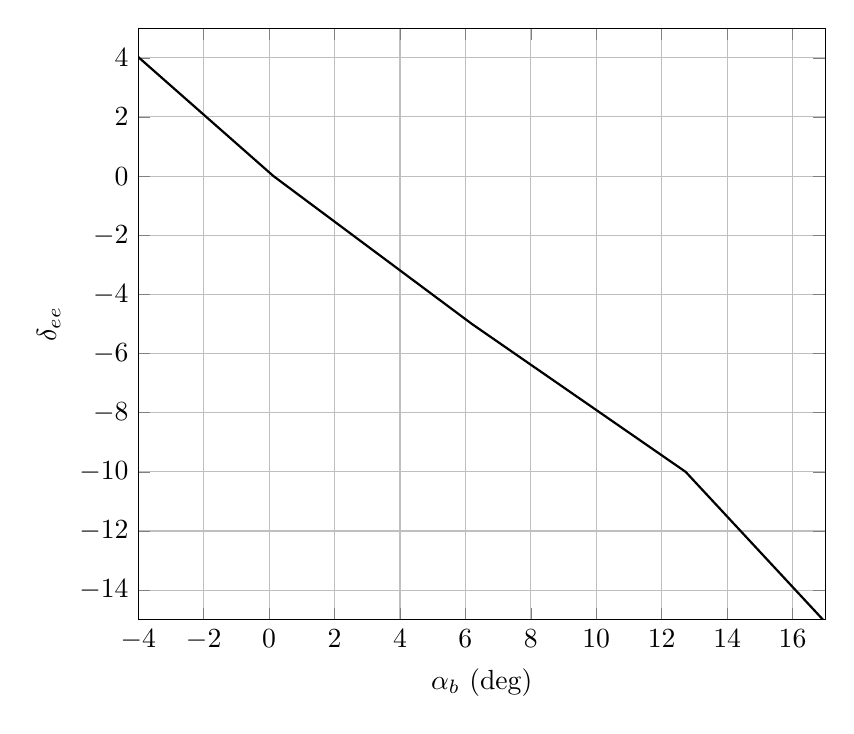
\begin{tikzpicture}

\begin{axis}[
width=0.85\textwidth,
height=0.75\textwidth,
scaled ticks=false, tick label style={/pgf/number format/fixed},
xmin=-4,
xmax=17,
xlabel={$\alpha_{b}$ (deg)},
xmajorgrids,
ymin=-15,
ymax=5,
ylabel={$\delta_{ee}$ },
ymajorgrids,
]

\addplot [
color=black,
thick
]
table[row sep=crcr]{
-4.999999999999999	5.0\\
-4.533333333333332	4.545454545454545\\
-4.0666666666666655	4.090909090909091\\
-3.5999999999999988	3.6363636363636362\\
-3.133333333333332	3.1818181818181817\\
-2.666666666666665	2.727272727272727\\
-2.1999999999999984	2.2727272727272725\\
-1.7333333333333318	1.818181818181818\\
-1.2666666666666653	1.3636363636363638\\
-0.7999999999999987	0.9090909090909092\\
-0.33333333333333215	0.45454545454545503\\
0.13333333333333441	0.0\\
0.600000000000001	-0.3846153846153845\\
1.0666666666666675	-0.769230769230769\\
1.533333333333334	-1.1538461538461535\\
2.000000000000001	-1.5384615384615383\\
2.4666666666666677	-1.9230769230769227\\
2.9333333333333345	-2.3076923076923075\\
3.4000000000000012	-2.692307692307692\\
3.866666666666668	-3.0769230769230766\\
4.333333333333335	-3.4615384615384617\\
4.800000000000002	-3.8461538461538463\\
5.266666666666668	-4.230769230769231\\
5.733333333333335	-4.615384615384616\\
6.200000000000002	-5.0\\
6.666666666666669	-5.357142857142858\\
7.1333333333333355	-5.714285714285714\\
7.600000000000002	-6.071428571428571\\
8.066666666666668	-6.428571428571428\\
8.533333333333335	-6.785714285714286\\
9.000000000000002	-7.142857142857142\\
9.466666666666669	-7.5\\
9.933333333333335	-7.857142857142858\\
10.400000000000002	-8.214285714285715\\
10.866666666666669	-8.571428571428571\\
11.333333333333336	-8.928571428571429\\
11.800000000000002	-9.285714285714285\\
12.26666666666667	-9.642857142857142\\
12.733333333333336	-10.0\\
13.200000000000003	-10.555555555555555\\
13.66666666666667	-11.111111111111112\\
14.133333333333336	-11.666666666666668\\
14.600000000000003	-12.222222222222225\\
15.06666666666667	-12.77777777777778\\
15.533333333333337	-13.333333333333336\\
16.000000000000004	-13.888888888888893\\
16.46666666666667	-14.444444444444446\\
16.933333333333334	-15.0\\
17.4	-20.0\\
17.866666666666664	-22.5\\
18.33333333333333	-25.0\\
18.799999999999994	-25.0\\
19.26666666666666	-25.0\\
19.733333333333324	-25.0\\
20.19999999999999	-25.0\\
20.666666666666654	-25.0\\
21.13333333333332	-25.0\\
21.599999999999984	-25.0\\
22.06666666666665	-25.0\\
22.533333333333314	-25.0\\
22.999999999999993	-25.0\\
};
\end{axis}
\end{tikzpicture}%
\caption{ATR 72 . Mach 0.45. $\delta_{ee}$ of elevator.}
\label{fig:stallATR}
\end{figure}
\noindent\\
\begin{figure}[H]
\centering
%CL vs Alpha clean WING
\begin{tikzpicture}

\begin{axis}[
width=0.85\textwidth,
height=0.75\textwidth,
scaled ticks=false, tick label style={/pgf/number format/fixed},
xmin=-5,
xmax=31,
xlabel={$\alpha$},
xmajorgrids,
ymin=-0.12,
ymax=0.18,
ylabel={C_M},
ymajorgrids,
]

\addplot [
color=black,
thick
]
table[row sep=crcr]{
-4.999999999999999	-0.0346499978751543\\
-4.416666666666666	-0.03683224247078975\\
-3.833333333333333	-0.03901448706642522\\
-3.25	-0.04119673166206068\\
-2.666666666666667	-0.04337897625769615\\
-2.083333333333334	-0.045561220853331606\\
-1.5000000000000007	-0.04774342494036219\\
-0.9166666666666674	-0.04992566026830355\\
-0.33333333333333415	-0.05210789778648536\\
0.2499999999999991	-0.054290133450387024\\
0.8333333333333324	-0.05647236911428868\\
1.4166666666666656	-0.058654604778190254\\
1.999999999999999	-0.06083684044209197\\
2.583333333333332	-0.06301907610599361\\
3.166666666666665	-0.06520131176989526\\
3.7499999999999982	-0.06738354743379686\\
4.333333333333331	-0.06956578309769854\\
4.916666666666664	-0.07174801876160013\\
5.499999999999997	-0.07393025442550175\\
6.08333333333333	-0.07611249008940348\\
6.666666666666663	-0.07829472575330497\\
7.2499999999999964	-0.08047696141720667\\
7.8333333333333295	-0.08265919708110829\\
8.416666666666663	-0.08484143274500995\\
8.999999999999996	-0.0870236684089117\\
9.58333333333333	-0.08920601849542838\\
10.166666666666664	-0.09142913966899054\\
10.749999999999998	-0.09374597584794751\\
11.333333333333332	-0.09613489552976402\\
11.916666666666666	-0.09853713513754958\\
12.5	-0.10088326257373548\\
13.083333333333334	-0.10309650060141236\\
13.666666666666668	-0.10509945845516959\\
14.250000000000002	-0.10682022225995143\\
14.833333333333336	-0.10818552134638938\\
15.41666666666667	-0.10912386437892152\\
16.000000000000004	-0.1095674226284545\\
16.583333333333336	-0.10945216369064258\\
17.166666666666668	-0.10871797918517158\\
17.75	-0.10730835832580536\\
18.333333333333332	-0.10517196742563517\\
18.916666666666664	-0.10226130828236642\\
19.499999999999996	-0.09852886243196447\\
20.08333333333333	-0.09393067375573365\\
20.66666666666666	-0.0884254230944664\\
21.249999999999993	-0.08196096710814749\\
21.833333333333325	-0.07448330243321331\\
22.416666666666657	-0.06593842570610088\\
22.99999999999999	-0.05627233356324668\\
23.58333333333332	-0.04543102264108795\\
24.166666666666654	-0.03336048957606038\\
24.749999999999986	-0.020006731004601302\\
25.333333333333318	-0.0053157403623828176\\
25.91666666666665	0.010766479410288644\\
26.499999999999982	0.028293931383998605\\
27.083333333333314	0.04732062561681688\\
27.666666666666647	0.06790056217388324\\
28.24999999999998	0.0900877444187615\\
28.83333333333331	0.11393617571501384\\
29.416666666666643	0.13949926083098416\\
29.999999999999993	0.16683218057094348\\
};
\end{axis}
\end{tikzpicture}%

\caption{ATR 72 . Mach 0.45. Neutral Point, stick fixed, $\delta_e = 0 $.}
\label{fig:stallATR}
\end{figure}
\begin{figure}[H]
\centering
%Comparison of CD estimation
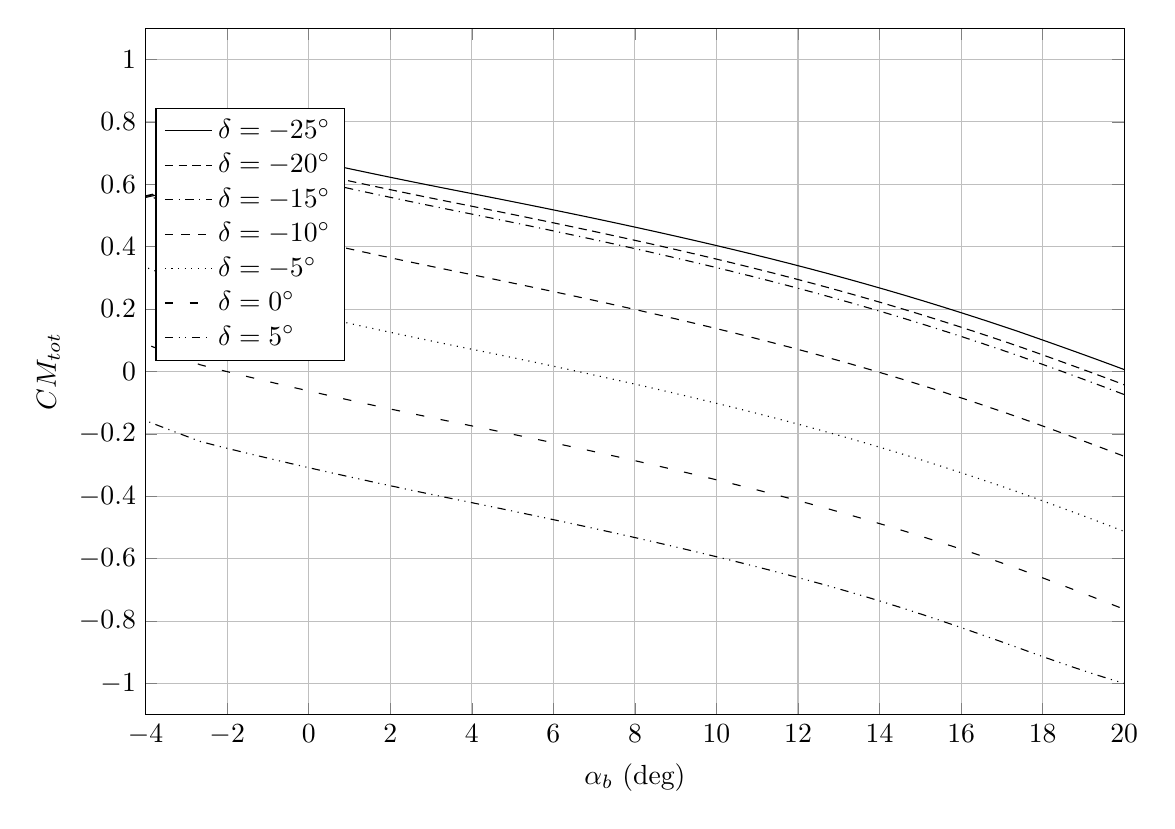
\begin{tikzpicture}

\begin{axis}[
width=14.01cm,
height=10.3cm,
scaled ticks=false, tick label style={/pgf/number format/fixed},
xmin=-4,
xmax=20,
xlabel={$\alpha_{b}$ (deg)},
xmajorgrids,
ymin=-1.1,
ymax=1.1,
ylabel={$CM_{tot}$},
ymajorgrids,
legend style={at={(0.01,0.7)},anchor=west,draw=black,fill=white,legend cell align=left},
legend entries = {$\delta = -25^{\circ}$\\$\delta = -20^{\circ}$\\$\delta = -15^{\circ}$\\$\delta = -10^{\circ}$\\$\delta = -5^{\circ}$\\$\delta = 0^{\circ}$\\$\delta = 5^{\circ}$\\}
]

\addplot [
color=black,
solid
]
table[row sep=crcr]{
-4.999999999999999	0.5297988693742903\\
-4.533333333333332	0.5427395318043312\\
-4.0666666666666655	0.5559097287501461\\
-3.5999999999999988	0.5693092140149555\\
-3.133333333333332	0.5829378753122981\\
-2.666666666666665	0.5967954910181147\\
-2.1999999999999984	0.6107194359838445\\
-1.7333333333333318	0.6248173427790104\\
-1.2666666666666653	0.6391031214245889\\
-0.7999999999999987	0.6535761978710936\\
-0.33333333333333215	0.668235455892315\\
0.13333333333333441	0.6741974536207279\\
0.600000000000001	0.6609128320640095\\
1.0666666666666675	0.6478402309293294\\
1.533333333333334	0.6349737462618468\\
2.000000000000001	0.6223071035097011\\
2.4666666666666677	0.6098337236393204\\
2.9333333333333345	0.5975474546213164\\
3.4000000000000012	0.5854420421115738\\
3.866666666666668	0.5734933586587739\\
4.333333333333335	0.5615387050224235\\
4.800000000000002	0.5494717026037501\\
5.266666666666668	0.5372778427649667\\
5.733333333333335	0.5249452651045265\\
6.200000000000002	0.5124534323740639\\
6.666666666666669	0.49979714980474577\\
7.1333333333333355	0.48696446161161194\\
7.600000000000002	0.47394229331715604\\
8.066666666666668	0.4607174992940666\\
8.533333333333335	0.4472764445969265\\
9.000000000000002	0.43359985847559646\\
9.466666666666669	0.4196740177408692\\
9.933333333333335	0.4054894698733661\\
10.400000000000002	0.3910315736573099\\
10.866666666666669	0.37628299213025457\\
11.333333333333336	0.3612015025200132\\
11.800000000000002	0.34575573152535083\\
12.26666666666667	0.32992556860096167\\
12.733333333333336	0.31370840268490985\\
13.200000000000003	0.29709128085192077\\
13.66666666666667	0.2800604878102902\\
14.133333333333336	0.26260247543001053\\
14.600000000000003	0.24470256996465506\\
15.06666666666667	0.22633604753554187\\
15.533333333333337	0.2075153809816243\\
16.000000000000004	0.1883118812531293\\
16.46666666666667	0.16870797217975209\\
16.933333333333334	0.14867363868254546\\
17.4	0.1281542991998242\\
17.866666666666664	0.10682813638754839\\
18.33333333333333	0.08528940627136923\\
18.799999999999994	0.06350186339721871\\
19.26666666666666	0.04142888362320825\\
19.733333333333324	0.019033079964673117\\
20.19999999999999	-0.003723408509451194\\
20.666666666666654	-0.026879517653611053\\
21.13333333333332	-0.050473392856676465\\
21.599999999999984	-0.07454386497426294\\
22.06666666666665	-0.0991281800351439\\
22.533333333333314	-0.12426379770711607\\
22.999999999999993	0.0\\
};

\addplot [
color=black,
densely dashed
]
table[row sep=crcr]{
-4.999999999999999	0.5330002881479072\\
-4.533333333333332	0.5459409505779481\\
-4.0666666666666655	0.559111147523763\\
-3.5999999999999988	0.5725106327885723\\
-3.133333333333332	0.5861392940859149\\
-2.666666666666665	0.5999969097917315\\
-2.1999999999999984	0.6139208547574614\\
-1.7333333333333318	0.6280187615526273\\
-1.2666666666666653	0.6423045401982058\\
-0.7999999999999987	0.6567776166447103\\
-0.33333333333333215	0.6490683817039139\\
0.13333333333333441	0.635355416678034\\
0.600000000000001	0.6218612320091452\\
1.0666666666666675	0.6085794650523756\\
1.533333333333334	0.5955042132070164\\
2.000000000000001	0.5826292032207252\\
2.4666666666666677	0.5699478573034837\\
2.9333333333333345	0.5574540303660354\\
3.4000000000000012	0.5451414764989649\\
3.866666666666668	0.5329859391140568\\
4.333333333333335	0.520823606341901\\
4.800000000000002	0.5085475430493409\\
5.266666666666668	0.4961431897499969\\
5.733333333333335	0.48359865076145514\\
6.200000000000002	0.47089328576147677\\
6.666666666666669	0.45802192071941705\\
7.1333333333333355	0.4449725677631275\\
7.600000000000002	0.43173211430084363\\
8.066666666666668	0.418287375879386\\
8.533333333333335	0.4046246780031095\\
9.000000000000002	0.3907246642956856\\
9.466666666666669	0.37657357376195266\\
9.933333333333335	0.3621619491189003\\
10.400000000000002	0.34747510643583424\\
10.866666666666669	0.33249566524801694\\
11.333333333333336	0.3171813584829152\\
11.800000000000002	0.3015007525174492\\
12.26666666666667	0.28543362219010404\\
12.733333333333336	0.2689773879919792\\
13.200000000000003	0.25211904925691236\\
13.66666666666667	0.23484484210917325\\
14.133333333333336	0.21714116898593475\\
14.600000000000003	0.19899330585465153\\
15.06666666666667	0.18037639027882146\\
15.533333333333337	0.16130289977036766\\
16.000000000000004	0.1418441168589551\\
16.46666666666667	0.12198241150091105\\
16.933333333333334	0.10168771389092235\\
17.4	0.0809052077255952\\
17.866666666666664	0.059310612795047936\\
18.33333333333333	0.03750345056059752\\
18.799999999999994	0.015447475568175563\\
19.26666666666666	-0.006893936324106216\\
19.733333333333324	-0.029558172100912782\\
20.19999999999999	-0.052583092693308416\\
20.666666666666654	-0.0760076339557397\\
21.13333333333332	-0.09986994127707666\\
21.599999999999984	-0.12420884551293446\\
22.06666666666665	-0.14906159269208685\\
22.533333333333314	-0.17446564248233046\\
22.999999999999993	0.0\\
};

\addplot [
color=black,
dashdotted
]
table[row sep=crcr]{
-4.999999999999999	0.5349311748540726\\
-4.533333333333332	0.5478718372841134\\
-4.0666666666666655	0.5610420342299282\\
-3.5999999999999988	0.5744415194947377\\
-3.133333333333332	0.5880701807920803\\
-2.666666666666665	0.6019277964978968\\
-2.1999999999999984	0.6158517414636268\\
-1.7333333333333318	0.6299496482587926\\
-1.2666666666666653	0.6442354269043711\\
-0.7999999999999987	0.6394253935742066\\
-0.33333333333333215	0.6253251489178525\\
0.13333333333333441	0.611453934328526\\
0.600000000000001	0.5978018027507768\\
1.0666666666666675	0.584362388321147\\
1.533333333333334	0.5711297894595329\\
2.000000000000001	0.5580977338930326\\
2.4666666666666677	0.5452596447688908\\
2.9333333333333345	0.5326093822286007\\
3.4000000000000012	0.520140706719948\\
3.866666666666668	0.5078292643247363\\
4.333333333333335	0.49551040458943524\\
4.800000000000002	0.48307677292307055\\
5.266666666666668	0.4705137715148749\\
5.733333333333335	0.45780947809138073\\
6.200000000000002	0.444943174643969\\
6.666666666666669	0.4319097027722876\\
7.1333333333333355	0.4186970504201976\\
7.600000000000002	0.40529207626936553\\
8.066666666666668	0.39168156660370523\\
8.533333333333335	0.3778518171187172\\
9.000000000000002	0.3637834069019448\\
9.466666666666669	0.3494625464640243\\
9.933333333333335	0.3348797749316144\\
10.400000000000002	0.3200203761799528\\
10.866666666666669	0.30486693695679284\\
11.333333333333336	0.28937715680060094\\
11.800000000000002	0.27351955662395583\\
12.26666666666667	0.2572738248795483\\
12.733333333333336	0.24063740583987872\\
13.200000000000003	0.22359726285666195\\
13.66666666666667	0.20613959543657476\\
14.133333333333336	0.18825076875946448\\
14.600000000000003	0.16991602089233238\\
15.06666666666667	0.1511103849681824\\
15.533333333333337	0.13184634202093654\\
16.000000000000004	0.11219515315979195\\
16.46666666666667	0.09213914773692661\\
16.933333333333334	0.07164821469997618\\
17.4	0.05066736082162735\\
17.866666666666664	0.028870449639518604\\
18.33333333333333	0.006860971153506545\\
18.799999999999994	-0.015397320090476717\\
19.26666666666666	-0.03794104823432003\\
19.733333333333324	-0.06080760026268835\\
20.19999999999999	-0.08403483710664528\\
20.666666666666654	-0.10766169462063821\\
21.13333333333332	-0.13172631819353658\\
21.599999999999984	-0.15626753868095603\\
22.06666666666665	-0.18132260211166973\\
22.533333333333314	-0.20692896815347486\\
22.999999999999993	0.0\\
};

\addplot [
color=black,
dashed
]
table[row sep=crcr]{
-4.999999999999999	0.5354683255799859\\
-4.533333333333332	0.5484089880100267\\
-4.0666666666666655	0.5615791849558415\\
-3.5999999999999988	0.5523515110031175\\
-3.133333333333332	0.5291587679681435\\
-2.666666666666665	0.5061949793416436\\
-2.1999999999999984	0.4903442613370192\\
-1.7333333333333318	0.475424071832094\\
-1.2666666666666653	0.4607451925453787\\
-0.7999999999999987	0.4463072707878443\\
-0.33333333333333215	0.43210940522839153\\
0.13333333333333441	0.41814075858007227\\
0.600000000000001	0.4043913812835569\\
1.0666666666666675	0.3908549054937487\\
1.533333333333334	0.37752543025891633\\
2.000000000000001	0.3643966839091863\\
2.4666666666666677	0.35146209016886215\\
2.9333333333333345	0.33871551239993775\\
3.4000000000000012	0.3261507149642391\\
3.866666666666668	0.31374328401885193\\
4.333333333333335	0.3013280528056461\\
4.800000000000002	0.2887974084792935\\
5.266666666666668	0.2761367296332327\\
5.733333333333335	0.2633340776222543\\
6.200000000000002	0.25036868660731293\\
6.666666666666669	0.23723540781141128\\
7.1333333333333355	0.22392221428866294\\
7.600000000000002	0.2104159470341849\\
8.066666666666668	0.19670337431512547\\
8.533333333333335	0.18277077347408743\\
9.000000000000002	0.16859868386461613\\
9.466666666666669	0.15417329845386332\\
9.933333333333335	0.13948515415797078\\
10.400000000000002	0.12451951503073548\\
10.866666666666669	0.10925894763309647\\
11.333333333333336	0.09366113094637667\\
11.800000000000002	0.07769455789139076\\
12.26666666666667	0.06133886373429531\\
12.733333333333336	0.04459150738946907\\
13.200000000000003	0.027439430054933635\\
13.66666666666667	0.00986880869242194\\
14.133333333333336	-0.008134014457036447\\
14.600000000000003	-0.02658382466122312\\
15.06666666666667	-0.045505653083539495\\
15.533333333333337	-0.06488701652161794\\
16.000000000000004	-0.08465666705454561\\
16.46666666666667	-0.10483230032955565\\
16.933333333333334	-0.12544405279424897\\
17.4	-0.1465470266055399\\
17.866666666666664	-0.16846850109466824\\
18.33333333333333	-0.1906025428876998\\
18.799999999999994	-0.21298539743870287\\
19.26666666666666	-0.23565368888956564\\
19.733333333333324	-0.25864480422495356\\
20.19999999999999	-0.2819966043759302\\
20.666666666666654	-0.3057480251969426\\
21.13333333333332	-0.3299372120768608\\
21.599999999999984	-0.3546059397474175\\
22.06666666666665	-0.379825730146919\\
22.533333333333314	-0.40566502041950436\\
22.999999999999993	0.0\\
};

\addplot [
color=black,
dotted
]
table[row sep=crcr]{
-4.999999999999999	0.3850611434135753\\
-4.533333333333332	0.3611378991793802\\
-4.0666666666666655	0.3374441894609591\\
-3.5999999999999988	0.3139797680615328\\
-3.133333333333332	0.2907445226946396\\
-2.666666666666665	0.2677382317362204\\
-2.1999999999999984	0.25185314533551506\\
-1.7333333333333318	0.236899460726778\\
-1.2666666666666653	0.22218714801926628\\
-0.7999999999999987	0.20771585477946303\\
-0.33333333333333215	0.19348467992431934\\
0.13333333333333441	0.1794827884159369\\
0.600000000000001	0.16570022984063548\\
1.0666666666666675	0.1521306356771622\\
1.533333333333334	0.13876810518819305\\
2.000000000000001	0.1256063669096141\\
2.4666666666666677	0.11263884476262802\\
2.9333333333333345	0.09985940320809726\\
3.4000000000000012	0.08726180794336073\\
3.866666666666668	0.0748216246785497\\
4.333333333333335	0.06237351048688536\\
4.800000000000002	0.0498097644038932\\
5.266666666666668	0.03711575697187483\\
5.733333333333335	0.024279543959407325\\
6.200000000000002	0.011280343207192883\\
6.666666666666669	-0.0018869907781746964\\
7.1333333333333355	-0.015234490023122518\\
7.600000000000002	-0.028775319567373565\\
8.066666666666668	-0.04252271729129236\\
8.533333333333335	-0.05649041211448112\\
9.000000000000002	-0.07069787824105933\\
9.466666666666669	-0.0851589286898998\\
9.933333333333335	-0.09988302729911248\\
10.400000000000002	-0.11488491677818809\\
10.866666666666669	-0.1301820374541443\\
11.333333333333336	-0.14581671735997556\\
11.800000000000002	-0.1618204731259561\\
12.26666666666667	-0.17821368763374332\\
12.733333333333336	-0.19499889697299294\\
13.200000000000003	-0.21218916750476088\\
13.66666666666667	-0.2297983299598895\\
14.133333333333336	-0.2478400499243191\\
14.600000000000003	-0.26632912062790887\\
15.06666666666667	-0.2852905951726812\\
15.533333333333337	-0.3047119896163711\\
16.000000000000004	-0.3245220605380496\\
16.46666666666667	-0.34473851211501627\\
16.933333333333334	-0.365391489459998\\
17.4	-0.38653613189785374\\
17.866666666666664	-0.40850010871890113\\
18.33333333333333	-0.43067799159953274\\
18.799999999999994	-0.4531110783489024\\
19.26666666666666	-0.4759124842014605\\
19.733333333333324	-0.4991609567047591\\
20.19999999999999	-0.5229137167474106\\
20.666666666666654	-0.5472171906576263\\
21.13333333333332	-0.5721194420734007\\
21.599999999999984	-0.5975684732703236\\
22.06666666666665	-0.6235058233411939\\
22.533333333333314	-0.6498788742608675\\
22.999999999999993	0.0\\
};

\addplot [
color=black,
loosely dashed
]
table[row sep=crcr]{
-4.999999999999999	0.13875658818898565\\
-4.533333333333332	0.11487388449215764\\
-4.0666666666666655	0.09122071531110358\\
-3.5999999999999988	0.06779683444904412\\
-3.133333333333332	0.04460212961951781\\
-2.666666666666665	0.021636379198465606\\
-2.1999999999999984	0.0057840748401246\\
-1.7333333333333318	-0.009137660709669556\\
-1.2666666666666653	-0.023818083194129924\\
-0.7999999999999987	-0.038257545290492065\\
-0.33333333333333215	-0.052456948318405375\\
0.13333333333333441	-0.06642712946100807\\
0.600000000000001	-0.08017803831706431\\
1.0666666666666675	-0.0937160427628804\\
1.533333333333334	-0.10704704374029116\\
2.000000000000001	-0.12017731290967285\\
2.4666666666666677	-0.13311342653763333\\
2.9333333333333345	-0.14586152121145832\\
3.4000000000000012	-0.15842783250767775\\
3.866666666666668	-0.17083677521298296\\
4.333333333333335	-0.18325352421698018\\
4.800000000000002	-0.19578569643234303\\
5.266666666666668	-0.20844791363725187\\
5.733333333333335	-0.22125211473476086\\
6.200000000000002	-0.23421906631721456\\
6.666666666666669	-0.24735391701004877\\
7.1333333333333355	-0.26066869399365417\\
7.600000000000002	-0.2741765565514657\\
8.066666666666668	-0.28789073670008786\\
8.533333333333335	-0.3018249573859648\\
9.000000000000002	-0.3159986798813368\\
9.466666666666669	-0.33042571149535127\\
9.933333333333335	-0.3451155153466803\\
10.400000000000002	-0.3600828276937026\\
10.866666666666669	-0.3753450822934085\\
11.333333333333336	-0.390944600488238\\
11.800000000000002	-0.40691288979822854\\
12.26666666666667	-0.42327031579487895\\
12.733333333333336	-0.4400194193332092\\
13.200000000000003	-0.45717325956410554\\
13.66666666666667	-0.4747456598809033\\
14.133333333333336	-0.49275027840384505\\
14.600000000000003	-0.5112019007682207\\
15.06666666666667	-0.5301255784849476\\
15.533333333333337	-0.5495232911043332\\
16.000000000000004	-0.5693409193321363\\
16.46666666666667	-0.589692498633693\\
16.933333333333334	-0.6106473011238349\\
17.4	-0.6322536995617907\\
17.866666666666664	-0.6548516534599129\\
18.33333333333333	-0.6778281147581244\\
18.799999999999994	-0.7011343122804665\\
19.26666666666666	-0.7246966867726682\\
19.733333333333324	-0.7484637154322333\\
20.19999999999999	-0.7723753642007253\\
20.666666666666654	-0.7961230261164166\\
21.13333333333332	-0.819630775448899\\
21.599999999999984	-0.8427739714762207\\
22.06666666666665	-0.8654051989998985\\
22.533333333333314	-0.887110515232329\\
22.999999999999993	0.0\\
};

\addplot [
color=black,
dashdotdotted
]
table[row sep=crcr]{
-4.999999999999999	-0.10667923837240866\\
-4.533333333333332	-0.1306024826066036\\
-4.0666666666666655	-0.15429619232502462\\
-3.5999999999999988	-0.17776061372445098\\
-3.133333333333332	-0.20099585909134426\\
-2.666666666666665	-0.22400215004976343\\
-2.1999999999999984	-0.2398872364504688\\
-1.7333333333333318	-0.2548409210592058\\
-1.2666666666666653	-0.2695532337667176\\
-0.7999999999999987	-0.28402452700652087\\
-0.33333333333333215	-0.2982557018616645\\
0.13333333333333441	-0.312257593370047\\
0.600000000000001	-0.3260401519453483\\
1.0666666666666675	-0.33960974610882166\\
1.533333333333334	-0.3529722765977908\\
2.000000000000001	-0.3661340148763698\\
2.4666666666666677	-0.37910153702335586\\
2.9333333333333345	-0.3918809785778867\\
3.4000000000000012	-0.4044785738426232\\
3.866666666666668	-0.4169187571074342\\
4.333333333333335	-0.42936687129909845\\
4.800000000000002	-0.44193061738209066\\
5.266666666666668	-0.454624624814109\\
5.733333333333335	-0.46746083782657655\\
6.200000000000002	-0.4804600385787909\\
6.666666666666669	-0.49362737256415856\\
7.1333333333333355	-0.5069748718091065\\
7.600000000000002	-0.5205157013533576\\
8.066666666666668	-0.5342630990772763\\
8.533333333333335	-0.5482307939004649\\
9.000000000000002	-0.562438260027043\\
9.466666666666669	-0.5768993104758836\\
9.933333333333335	-0.5916234090850964\\
10.400000000000002	-0.6066252985641719\\
10.866666666666669	-0.6219224192401283\\
11.333333333333336	-0.6375570991459596\\
11.800000000000002	-0.6535625686371799\\
12.26666666666667	-0.6699729574798405\\
12.733333333333336	-0.6868283415930607\\
13.200000000000003	-0.7042217724034161\\
13.66666666666667	-0.7221533613106607\\
14.133333333333336	-0.7406781879119004\\
14.600000000000003	-0.7598743865391371\\
15.06666666666667	-0.779671321101776\\
15.533333333333337	-0.800044089394422\\
16.000000000000004	-0.8208949713644969\\
16.46666666666667	-0.8421088131089535\\
16.933333333333334	-0.8636290754308678\\
17.4	-0.8854244953948567\\
17.866666666666664	-0.9075225313130479\\
18.33333333333333	-0.9290886954984583\\
18.799999999999994	-0.950045495512345\\
19.26666666666666	-0.9702532916211043\\
19.733333333333324	-0.9893605541985829\\
20.19999999999999	-1.0067203760133434\\
20.666666666666654	-1.0224958323653088\\
21.13333333333332	-1.0364710329819904\\
21.599999999999984	-1.0484242708475515\\
22.06666666666665	-1.0567648141114652\\
22.533333333333314	-1.0620436869609138\\
22.999999999999993	0.0\\
};
\end{axis}
\end{tikzpicture}%

\caption{ATR 72 . Mach 0.2. TakeOff Conditions. $CM_{tot}$ vs $\alpha_b$ with elevator deflection.}
\label{fig:stallATR}
\end{figure}
\noindent\\
\begin{figure}[H]
\centering
%Comparison of CD estimation
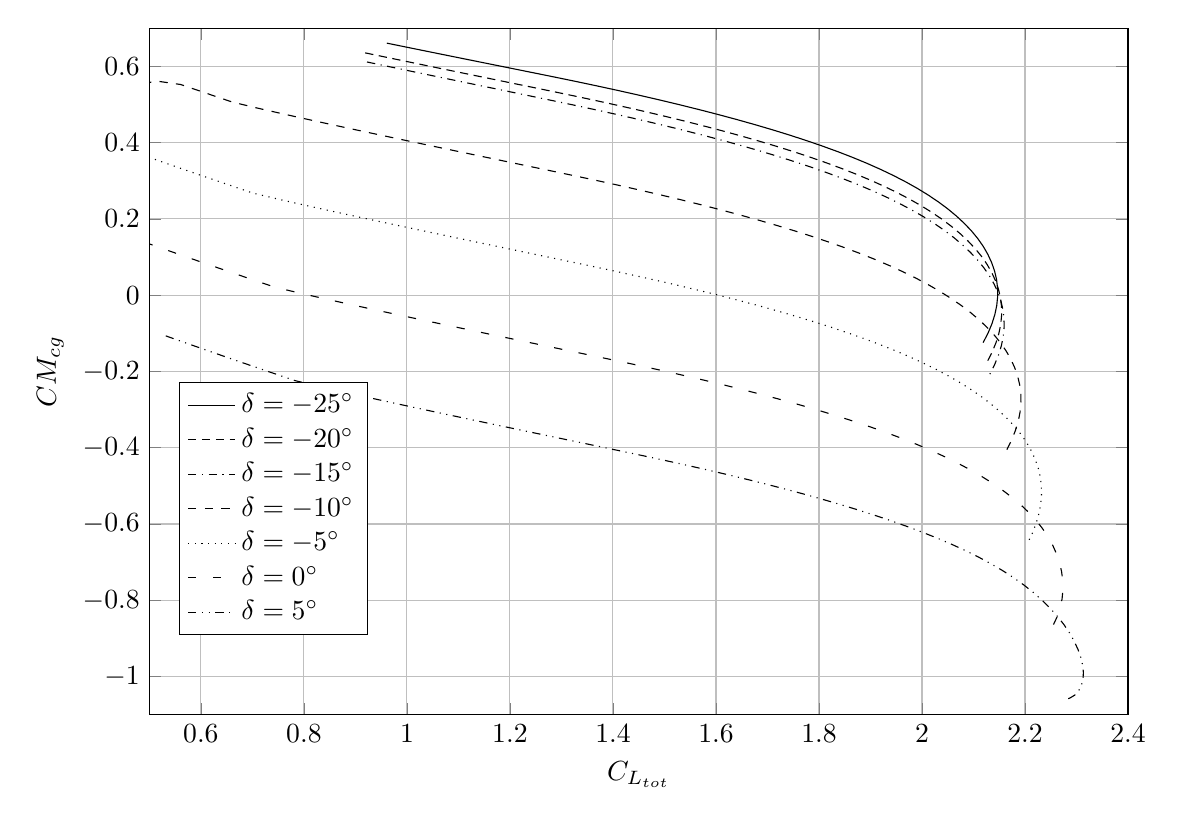
\begin{tikzpicture}

\begin{axis}[
width=14.01cm,
height=10.3cm,
scaled ticks=false, tick label style={/pgf/number format/fixed},
xmin=0.5,
xmax=2.4,
xlabel={$C_{L_{tot}}$},
xmajorgrids,
ymin=-1.1,
ymax=0.7,
ylabel={$CM_{cg}$},
ymajorgrids,
legend style={at={(0.03,0.3)},anchor=west,draw=black,fill=white,legend cell align=left},
legend entries = {$\delta = -25^{\circ}$\\$\delta = -20^{\circ}$\\$\delta = -15^{\circ}$\\$\delta = -10^{\circ}$\\$\delta = -5^{\circ}$\\$\delta = 0^{\circ}$\\$\delta = 5^{\circ}$\\}
]

\addplot [
color=black,
solid
]
table[row sep=crcr]{
0.9609125231577784	0.6609128320640095\\
1.008398709311174	0.6478402309293294\\
1.0553527461672072	0.6349737462618468\\
1.1017414138822166	0.6223071035097011\\
1.1475314938730183	0.6098337236393204\\
1.1926896392492496	0.5975474546213164\\
1.237182469457526	0.5854420421115738\\
1.2809797025465355	0.5734933586587739\\
1.324073208306093	0.5615387050224235\\
1.3664423312976526	0.5494717026037501\\
1.4080550262386187	0.5372778427649667\\
1.4488788972057947	0.5249452651045265\\
1.4888830752157993	0.5124534323740639\\
1.5280339025968996	0.49979714980474577\\
1.566298911492897	0.48696446161161194\\
1.603645769798642	0.47394229331715604\\
1.6400421614369773	0.4607174992940666\\
1.6754557866459165	0.4472764445969265\\
1.7098553834581258	0.43359985847559646\\
1.7432086128243662	0.4196740177408692\\
1.775482391464673	0.4054894698733661\\
1.8066444908971195	0.3910315736573099\\
1.8366627003742544	0.37628299213025457\\
1.86550482712366	0.3612015025200132\\
1.8931390392340979	0.34575573152535083\\
1.9195347276966752	0.32992556860096167\\
1.9446579912508115	0.31370840268490985\\
1.9684767146173319	0.29709128085192077\\
1.9909588015075352	0.2800604878102902\\
2.012072174750573	0.26260247543001053\\
2.031784776394926	0.24470256996465506\\
2.050066536682003	0.22633604753554187\\
2.0668841597859906	0.2075153809816243\\
2.0822050952652007	0.1883118812531293\\
2.0959973659657387	0.16870797217975209\\
2.1082290139462656	0.14867363868254546\\
2.1188721358517344	0.1281542991998242\\
2.1279490136138053	0.10682813638754839\\
2.135307860304551	0.08528940627136923\\
2.140915485350066	0.06350186339721871\\
2.1447386981764422	0.04142888362320825\\
2.146744308209773	0.019033079964673117\\
2.1468991248761506	-0.003723408509451194\\
2.145169957601668	-0.026879517653611053\\
2.1415236158124182	-0.050473392856676465\\
2.1359269089344934	-0.07454386497426294\\
2.128346646393988	-0.0991281800351439\\
2.118749637616993	-0.12426379770711607\\
};

\addplot [
color=black,
densely dashed
]
table[row sep=crcr]{
0.9189843450335926	0.635355416678034\\
0.9670044349846184	0.6218612320091452\\
1.0145255304053264	0.6085794650523756\\
1.061514409995922	0.5955042132070164\\
1.107937853695857	0.5826292032207252\\
1.1537626427144019	0.5699478573034837\\
1.1989554290029023	0.5574540303660354\\
1.243482830600243	0.5451414764989649\\
1.2873145871077463	0.5329859391140568\\
1.3304427540102892	0.520823606341901\\
1.372846768753561	0.5085475430493409\\
1.4144945945414737	0.4961431897499969\\
1.4553538413391207	0.48359865076145514\\
1.4953936573659004	0.47089328576147677\\
1.534580381488926	0.45802192071941705\\
1.5728815512072731	0.4449725677631275\\
1.6102648407769693	0.43173211430084363\\
1.6466979406007998	0.418287375879386\\
1.6821485575176154	0.4046246780031095\\
1.716585443850885	0.3907246642956856\\
1.7499762668610919	0.37657357376195266\\
1.7822879440633095	0.3621619491189003\\
1.8134882541046276	0.34747510643583424\\
1.8435449934980206	0.33249566524801694\\
1.8724259768646918	0.3171813584829152\\
1.9000993823609718	0.3015007525174492\\
1.926534620107134	0.28543362219010404\\
1.9516977835764737	0.2689773879919792\\
1.9755567654576538	0.25211904925691236\\
1.9980794775705295	0.23484484210917325\\
2.019233850994469	0.21714116898593475\\
2.0389878361705844	0.19899330585465153\\
2.057311386465248	0.18037639027882146\\
2.074171205272739	0.16130289977036766\\
2.0895347468946914	0.1418441168589551\\
2.103370043168546	0.12198241150091105\\
2.1156451452866603	0.10168771389092235\\
2.1263321890718085	0.0809052077255952\\
2.1354538675019734	0.059310612795047936\\
2.142857514860813	0.03750345056059752\\
2.1485099405744217	0.015447475568175563\\
2.152377954068892	-0.006893936324106216\\
2.154428364770316	-0.029558172100912782\\
2.154627982104788	-0.052583092693308416\\
2.1529436154983985	-0.0760076339557397\\
2.149342074377243	-0.09986994127707666\\
2.143790168167412	-0.12420884551293446\\
2.136254706295	-0.14906159269208685\\
2.126702498186099	-0.17446564248233046\\
};

\addplot [
color=black,
dashdotted
]
table[row sep=crcr]{
0.9225721455562089	0.611453934328526\\
0.970618596462421	0.5978018027507768\\
1.0181660028631745	0.584362388321147\\
1.0651811432883387	0.5711297894595329\\
1.1116307975138988	0.5580977338930326\\
1.1574817465926983	0.5452596447688908\\
1.2027006416030839	0.5326093822286007\\
1.2472540995229384	0.520140706719948\\
1.2911118761977218	0.5078292643247363\\
1.3342661670699623	0.49551040458943524\\
1.3766964795918397	0.48307677292307055\\
1.4183707833635129	0.4705137715148749\\
1.4592566927880575	0.45780947809138073\\
1.49932336905054	0.444943174643969\\
1.5385371484094161	0.4319097027722876\\
1.57686557240001	0.4186970504201976\\
1.614276320072744	0.40529207626936553\\
1.6507370867143116	0.39168156660370523\\
1.686215584138589	0.3778518171187172\\
1.7206805754399677	0.3637834069019448\\
1.7540997326345442	0.3494625464640243\\
1.7864399738366092	0.3348797749316144\\
1.8176690830663647	0.3200203761799528\\
1.8477548623089404	0.30486693695679284\\
1.8766651317580825	0.28937715680060094\\
1.9043680771580094	0.27351955662395583\\
1.9308331230465745	0.2572738248795483\\
1.9560263589280145	0.24063740583987872\\
1.979915683496321	0.22359726285666195\\
2.002469014682737	0.20613959543657476\\
2.023654289784787	0.18825076875946448\\
2.0434394655690773	0.16991602089233238\\
2.061794512831175	0.1511103849681824\\
2.078686134377548	0.13184634202093654\\
2.0940817880848526	0.11219515315979195\\
2.1079495125672643	0.09213914773692661\\
2.1202573659011725	0.07164821469997618\\
2.1309775134375237	0.05066736082162735\\
2.1401329579583286	0.028870449639518604\\
2.147570371407808	0.006860971153506545\\
2.1532565632120564	-0.015397320090476717\\
2.157158342797166	-0.03794104823432003\\
2.1592425195892306	-0.06080760026268835\\
2.159475903014342	-0.08403483710664528\\
2.1578253024985927	-0.10766169462063821\\
2.1542575274680766	-0.13172631819353658\\
2.1487393873488854	-0.15626753868095603\\
2.1412376915671136	-0.18132260211166973\\
2.131719249548852	-0.20692896815347486\\
};

\addplot [
color=black,
dashed
]
table[row sep=crcr]{
0.42509589167103656	0.5354683255799859\\
0.46914741028192375	0.5484089880100267\\
0.513198928892811	0.5615791849558415\\
0.5610268653799863	0.5523515110031175\\
0.611223786876572	0.5291587679681435\\
0.6614207083731577	0.5061949793416436\\
0.7104415458640999	0.4903442613370192\\
0.7593361142166708	0.475424071832094\\
0.8082217638355426	0.4607451925453787\\
0.8570984577761929	0.4463072707878443\\
0.9059511451474966	0.43210940522839153\\
0.9544798085936351	0.41814075858007227\\
1.0025424895739459	0.4043913812835569\\
1.0501060952797978	0.3908549054937487\\
1.097137404136186	0.37752543025891633\\
1.1436031958184527	0.3643966839091863\\
1.189470251283131	0.35146209016886215\\
1.2347052210710736	0.33871551239993775\\
1.2792747215069202	0.3261507149642391\\
1.32314851843742	0.31374328401885193\\
1.3663188934750843	0.3013280528056461\\
1.4087653971741168	0.2887974084792935\\
1.4504560030727567	0.2761367296332327\\
1.491358328306484	0.2633340776222543\\
1.5314415420431469	0.25036868660731293\\
1.5706719789350867	0.23723540781141128\\
1.60901718300269	0.22392221428866294\\
1.6464448362482216	0.2104159470341849\\
1.6829226369653292	0.19670337431512547\\
1.7184183000309428	0.18277077347408743\\
1.752900595170962	0.16859868386461613\\
1.7863371973294477	0.15417329845386332\\
1.8186950249896212	0.13948515415797078\\
1.849941865479834	0.12451951503073548\\
1.8800455241543468	0.10925894763309647\\
1.9089738246378425	0.09366113094637667\\
1.9366949573462975	0.07769455789139076\\
1.9631783556942677	0.06133886373429531\\
1.9883901067422962	0.04459150738946907\\
2.0122981128817723	0.027439430054933635\\
2.0348702958066354	0.00986880869242194\\
2.056074596642843	-0.008134014457036447\\
2.0758789760515195	-0.02658382466122312\\
2.0942534155591463	-0.045505653083539495\\
2.111164617610282	-0.06488701652161794\\
2.126580042282677	-0.08465666705454561\\
2.140467732362846	-0.10483230032955565\\
2.1527957501655837	-0.12544405279424897\\
2.163536279221921	-0.1465470266055399\\
2.172712513055906	-0.16846850109466824\\
2.1801707158185657	-0.1906025428876998\\
2.1858776969359948	-0.21298539743870287\\
2.189800265834285	-0.23565368888956564\\
2.1919052319395296	-0.25864480422495356\\
2.1921594046778217	-0.2819966043759302\\
2.190529593475253	-0.3057480251969426\\
2.1869826077579173	-0.3299372120768608\\
2.1814857482776757	-0.3546059397474175\\
2.174011545026612	-0.379825730146919\\
2.164531977496327	-0.40566502041950436\\
};

\addplot [
color=black,
dotted
]
table[row sep=crcr]{
0.4499264793720636	0.3850611434135753\\
0.5001304944045414	0.3611378991793802\\
0.5503345094370192	0.3374441894609591\\
0.600538524469497	0.3139797680615328\\
0.6507425395019746	0.2907445226946396\\
0.7009465545344524	0.2677382317362204\\
0.7499731280271653	0.25185314533551506\\
0.7988732866311499	0.236899460726778\\
0.84776451620669	0.22218714801926628\\
0.896646779766619	0.20771585477946303\\
0.9455050263784126	0.19348467992431934\\
0.9940392383108914	0.1794827884159369\\
1.0421074571659816	0.16570022984063548\\
1.0896765902479015	0.1521306356771622\\
1.1367134159458618	0.13876810518819305\\
1.1831847139008638	0.1256063669096141\\
1.2290572650365787	0.11263884476262802\\
1.274297719710461	0.09985940320809726\\
1.3188726940242563	0.08726180794336073\\
1.3627519572372608	0.0748216246785497\\
1.405927820364105	0.06237351048688536\\
1.4483798486658641	0.0498097644038932\\
1.4900760170244927	0.03711575697187483\\
1.5309839435077959	0.024279543959407325\\
1.5710728000074325	0.011280343207192883\\
1.6103089206277201	-0.0018869907781746964\\
1.6486598502369758	-0.015234490023122518\\
1.6860932718446642	-0.028775319567373565\\
1.722576884770438	-0.04252271729129236\\
1.7580784049363736	-0.05649041211448112\\
1.7925666043311126	-0.07069787824105933\\
1.8260091588977685	-0.0851589286898998\\
1.8583729872454453	-0.09988302729911248\\
1.889625877831271	-0.11488491677818809\\
1.919735637159089	-0.1301820374541443\\
1.9486700900242555	-0.14581671735997556\\
1.9763974284367998	-0.1618204731259561\\
2.002887088840104	-0.17821368763374332\\
2.0281051574608973	-0.19499889697299294\\
2.05201953795216	-0.21218916750476088\\
2.0745981532917033	-0.2297983299598895\\
2.095808945911788	-0.2478400499243191\\
2.115619877802389	-0.26632912062790887\\
2.1340009341514907	-0.2852905951726812\\
2.1509188172801643	-0.3047119896163711\\
2.166340988017197	-0.3245220605380496\\
2.1802354905727506	-0.34473851211501627\\
2.1925703887078076	-0.365391489459998\\
2.2033178721566395	-0.38653613189785374\\
2.2125011995265167	-0.40850010871890113\\
2.219966719260138	-0.43067799159953274\\
2.2256820840093807	-0.4531110783489024\\
2.229626869377769	-0.4759124842014605\\
2.2317747877688108	-0.4991609567047591\\
2.2320958797384582	-0.5229137167474106\\
2.2305582048546686	-0.5472171906576263\\
2.227130227875207	-0.5721194420734007\\
2.2217635991569256	-0.5975684732703236\\
2.2144091548709275	-0.6235058233411939\\
2.2050186706952934	-0.6498788742608675\\
};

\addplot [
color=black,
loosely dashed
]
table[row sep=crcr]{
0.4909359859598515	0.13875658818898565\\
0.5411332348751797	0.11487388449215764\\
0.591330483790508	0.09122071531110358\\
0.6415277327058362	0.06779683444904412\\
0.6917249816211645	0.04460212961951781\\
0.7419222305364926	0.021636379198465606\\
0.7909433327860144	0.0057840748401246\\
0.8398381591697162	-0.009137660709669556\\
0.8887240663445407	-0.023818083194129924\\
0.9376010173639974	-0.038257545290492065\\
0.9864539613350503	-0.052456948318405375\\
1.034982880884555	-0.06642712946100807\\
1.0830458174784305	-0.08017803831706431\\
1.1306096783132547	-0.0937160427628804\\
1.177641241812371	-0.10704704374029116\\
1.224107287649536	-0.12017731290967285\\
1.2699745967797664	-0.13311342653763333\\
1.31520981973545	-0.14586152121145832\\
1.359779572830938	-0.15842783250767775\\
1.4036536220704938	-0.17083677521298296\\
1.4468242504237518	-0.18325352421698018\\
1.4892710091237464	-0.19578569643234303\\
1.5309618717707392	-0.20844791363725187\\
1.5718644555432433	-0.22125211473476086\\
1.611947929734831	-0.23421906631721456\\
1.651178628972548	-0.24735391701004877\\
1.6895240973159198	-0.26066869399365417\\
1.7269520168137003	-0.2741765565514657\\
1.7634300858068948	-0.28789073670008786\\
1.7989260192206749	-0.3018249573859648\\
1.833408586885382	-0.3159986798813368\\
1.8668454637911909	-0.33042571149535127\\
1.8992035684271331	-0.3451155153466803\\
1.9304506881736616	-0.3600828276937026\\
1.9605546284380984	-0.3753450822934085\\
1.989483212899162	-0.390944600488238\\
2.0172046320464054	-0.40691288979822854\\
2.043688319434188	-0.42327031579487895\\
2.0689003620845656	-0.4400194193332092\\
2.09280866244716	-0.45717325956410554\\
2.115381142275169	-0.4747456598809033\\
2.136585742754847	-0.49275027840384505\\
2.156390424608655	-0.5112019007682207\\
2.174765172759024	-0.5301255784849476\\
2.1916791034487817	-0.5495232911043332\\
2.207102535481838	-0.5693409193321363\\
2.2210195905261867	-0.589692498633693\\
2.233404862544361	-0.6106473011238349\\
2.2442294119472748	-0.6322536995617907\\
2.2535185485503835	-0.6548516534599129\\
2.2611173490808905	-0.6778281147581244\\
2.266978433895977	-0.7011343122804665\\
2.2710502230807266	-0.7246966867726682\\
2.273284687233857	-0.7484637154322333\\
2.2736322973456553	-0.7723753642007253\\
2.272001858790925	-0.7961230261164166\\
2.268341142803211	-0.819630775448899\\
2.2625896757996395	-0.8427739714762207\\
2.2546834476963102	-0.8654051989998985\\
2.2445139299466774	-0.887110515232329\\
};

\addplot [
color=black,
dashdotdotted
]
table[row sep=crcr]{
0.5318005043230066	-0.10667923837240866\\
0.5820045193554844	-0.1306024826066036\\
0.6322085343879622	-0.15429619232502462\\
0.6824125494204399	-0.17776061372445098\\
0.7326165644529177	-0.20099585909134426\\
0.7828205794853954	-0.22400215004976343\\
0.8318471529781084	-0.2398872364504688\\
0.880747311582093	-0.2548409210592058\\
0.9296385411576331	-0.2695532337667176\\
0.978520804717562	-0.28402452700652087\\
1.0273790513293557	-0.2982557018616645\\
1.0759132632618345	-0.312257593370047\\
1.1239814821169247	-0.3260401519453483\\
1.1715506151988446	-0.33960974610882166\\
1.218587440896805	-0.3529722765977908\\
1.2650587388518069	-0.3661340148763698\\
1.3109312899875218	-0.37910153702335586\\
1.356171744661404	-0.3918809785778867\\
1.4007467189751994	-0.4044785738426232\\
1.444625982188204	-0.4169187571074342\\
1.487801845315048	-0.42936687129909845\\
1.5302538736168072	-0.44193061738209066\\
1.5719500419754358	-0.454624624814109\\
1.612857968458739	-0.46746083782657655\\
1.6529468249583754	-0.4804600385787909\\
1.6921829455786632	-0.49362737256415856\\
1.730533875187919	-0.5069748718091065\\
1.7679672967956073	-0.5205157013533576\\
1.8044509097213808	-0.5342630990772763\\
1.8399524298873167	-0.5482307939004649\\
1.8744406292820555	-0.562438260027043\\
1.9078831838487114	-0.5768993104758836\\
1.9402470121963884	-0.5916234090850964\\
1.971499902782214	-0.6066252985641719\\
2.001609662110032	-0.6219224192401283\\
2.0305441149751986	-0.6375570991459596\\
2.05827173940432	-0.6535625686371799\\
2.084764266162371	-0.6699729574798405\\
2.109994046782375	-0.6868283415930607\\
2.1339423342303365	-0.7042217724034161\\
2.1565747617610547	-0.7221533613106607\\
2.1778661837045936	-0.7406781879119004\\
2.1977951335269204	-0.7598743865391371\\
2.216315626122352	-0.779671321101776\\
2.233392291234026	-0.800044089394422\\
2.2489881708052613	-0.8208949713644969\\
2.2630491353555326	-0.8421088131089535\\
2.2755287812452343	-0.8636290754308678\\
2.286384877881411	-0.8854244953948567\\
2.2955905793887603	-0.9075225313130479\\
2.30295400475898	-0.9290886954984583\\
2.308422980840304	-0.950045495512345\\
2.3119348990464275	-0.9702532916211043\\
2.3133916595663915	-0.9893605541985829\\
2.312645785684351	-1.0067203760133434\\
2.3096848053981174	-1.0224958323653088\\
2.3044331301993575	-1.0364710329819904\\
2.2968140863766755	-1.0484242708475515\\
2.2865227778050414	-1.0567648141114652\\
2.273611726580572	-1.0620436869609138\\
};
\end{axis}
\end{tikzpicture}%
\caption{ATR 72 . Mach 0.2. TakeOff Conditions. $CM_{tot}$ vs $CL_{tot}$ with elevator deflection.}
\label{fig:stallATR}
\end{figure}

\subsection{Boeing 747-100B}

\begin{figure}[H]
\centering
% Moment Coefficient vs alpha for Wing respect to A C 
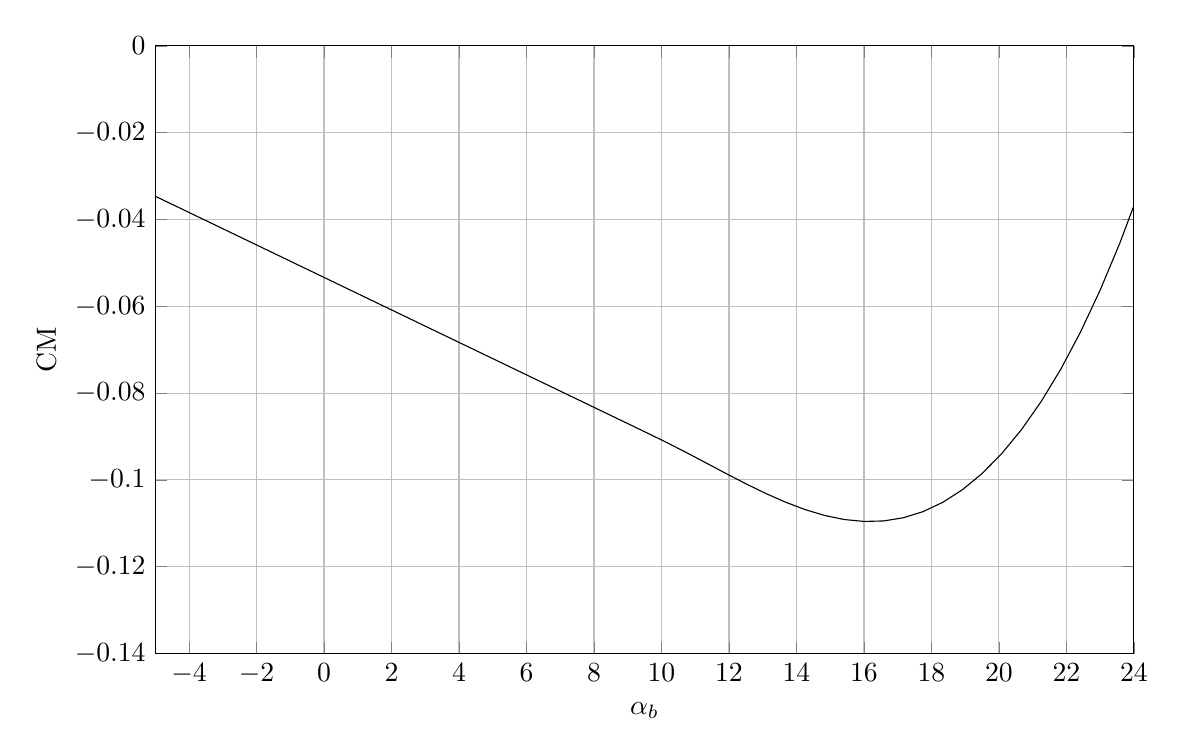
\begin{tikzpicture}

\begin{axis}[
width=14.01cm,
height=9.3cm,
scaled ticks=false, tick label style={/pgf/number format/fixed},
xmin=-5,
xmax=24,
xlabel={$\alpha_b$},
xmajorgrids,
ymin=-0.14,
ymax=0.0,
ylabel={CM},
ymajorgrids,
]
\addplot [
color=black,
solid
]
table[row sep=crcr]{
-4.999999999999999	-0.0346499978751543\\
-4.416666666666666	-0.03683224247078975\\
-3.833333333333333	-0.03901448706642522\\
-3.25	-0.04119673166206068\\
-2.666666666666667	-0.04337897625769615\\
-2.083333333333334	-0.045561220853331606\\
-1.5000000000000007	-0.04774342494036219\\
-0.9166666666666674	-0.04992566026830355\\
-0.33333333333333415	-0.05210789778648536\\
0.2499999999999991	-0.054290133450387024\\
0.8333333333333324	-0.05647236911428868\\
1.4166666666666656	-0.058654604778190254\\
1.999999999999999	-0.06083684044209197\\
2.583333333333332	-0.06301907610599361\\
3.166666666666665	-0.06520131176989526\\
3.7499999999999982	-0.06738354743379686\\
4.333333333333331	-0.06956578309769854\\
4.916666666666664	-0.07174801876160013\\
5.499999999999997	-0.07393025442550175\\
6.08333333333333	-0.07611249008940348\\
6.666666666666663	-0.07829472575330497\\
7.2499999999999964	-0.08047696141720667\\
7.8333333333333295	-0.08265919708110829\\
8.416666666666663	-0.08484143274500995\\
8.999999999999996	-0.0870236684089117\\
9.58333333333333	-0.08920601849542838\\
10.166666666666664	-0.09142913966899054\\
10.749999999999998	-0.09374597584794751\\
11.333333333333332	-0.09613489552976402\\
11.916666666666666	-0.09853713513754958\\
12.5	-0.10088326257373548\\
13.083333333333334	-0.10309650060141236\\
13.666666666666668	-0.10509945845516959\\
14.250000000000002	-0.10682022225995143\\
14.833333333333336	-0.10818552134638938\\
15.41666666666667	-0.10912386437892152\\
16.000000000000004	-0.1095674226284545\\
16.583333333333336	-0.10945216369064258\\
17.166666666666668	-0.10871797918517158\\
17.75	-0.10730835832580536\\
18.333333333333332	-0.10517196742563517\\
18.916666666666664	-0.10226130828236642\\
19.499999999999996	-0.09852886243196447\\
20.08333333333333	-0.09393067375573365\\
20.66666666666666	-0.0884254230944664\\
21.249999999999993	-0.08196096710814749\\
21.833333333333325	-0.07448330243321331\\
22.416666666666657	-0.06593842570610088\\
22.99999999999999	-0.05627233356324668\\
23.58333333333332	-0.04543102264108795\\
24.166666666666654	-0.03336048957606038\\
24.749999999999986	-0.020006731004601302\\
25.333333333333318	-0.0053157403623828176\\
25.91666666666665	0.010766479410288644\\
26.499999999999982	0.028293931383998605\\
27.083333333333314	0.04732062561681688\\
27.666666666666647	0.06790056217388324\\
28.24999999999998	0.0900877444187615\\
28.83333333333331	0.11393617571501384\\
29.416666666666643	0.13949926083098416\\
29.999999999999993	0.16683218057094348\\
};
\end{axis}
\end{tikzpicture}%

\caption{BOEING 747-100B . Mach 0.7. Pitching Moment Coefficient of the Wing respect to a quarter of MAC.}
\label{fig:stallATR}
\end{figure}
\noindent\\
\begin{figure}[H]
\centering
% Moment Coefficient vs alpha for Wing respect to A C 
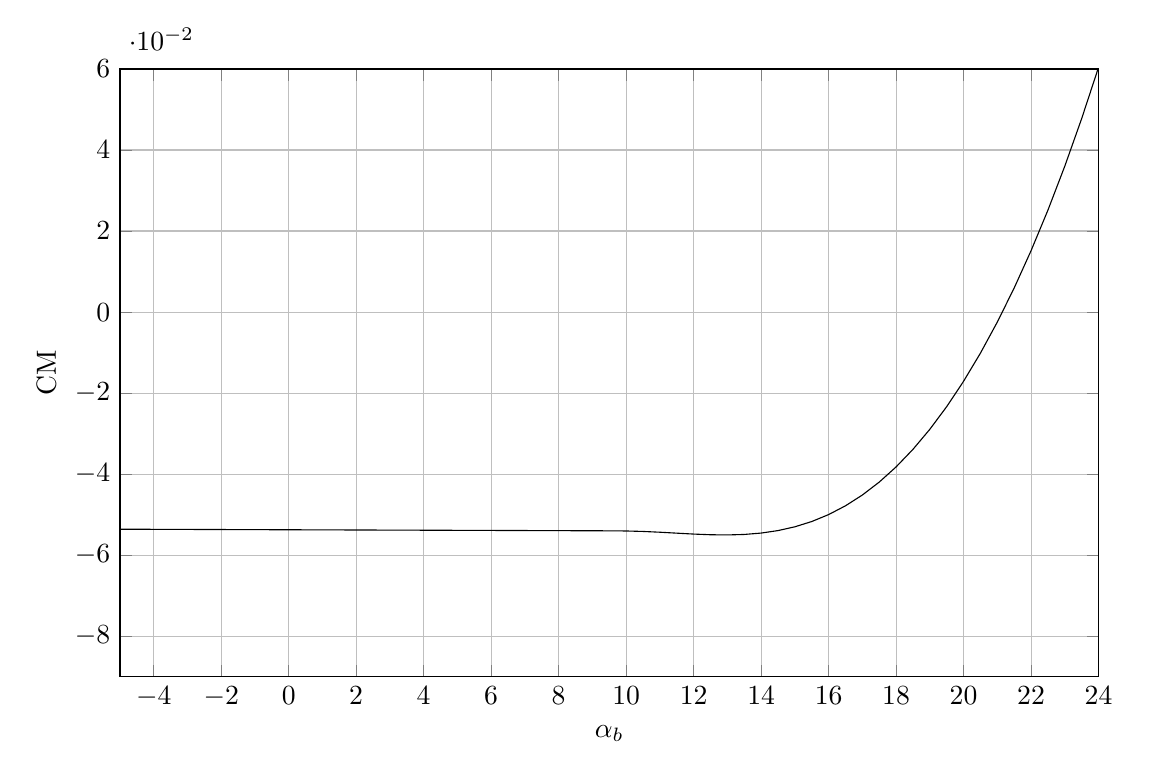
\begin{tikzpicture}

\begin{axis}[
width=14.01cm,
height=9.3cm,
xmin=-5,
xmax=24,
xlabel={$\alpha_b$},
xmajorgrids,
ymin=-0.09,
ymax=0.06,
ylabel={CM},
ymajorgrids,
]
\addplot [
color=black,
solid
]
table[row sep=crcr]{
-4.999999999999999	-0.05358690972706631\\
-4.499999999999999	-0.053600722675332134\\
-3.999999999999999	-0.05361453562359796\\
-3.499999999999999	-0.05362834857186379\\
-2.999999999999999	-0.0536421615201296\\
-2.499999999999999	-0.05365597446839545\\
-1.9999999999999991	-0.053669787416661285\\
-1.4999999999999991	-0.053683550357214206\\
-0.9999999999999991	-0.05369735577261873\\
-0.49999999999999917	-0.05371115931088905\\
7.771561172376096E-16	-0.053724962849159404\\
0.5000000000000007	-0.05373876638742973\\
1.0000000000000007	-0.053752569925700024\\
1.5000000000000007	-0.05376637346397039\\
2.0000000000000004	-0.053780177002240664\\
2.5000000000000004	-0.05379398054051104\\
3.0000000000000004	-0.053807784078781264\\
3.5000000000000004	-0.05382158761705166\\
4.0	-0.05383539115532191\\
4.5	-0.05384919469359232\\
5.0	-0.0538629982318626\\
5.5	-0.05387680177013284\\
6.0	-0.05389060530840325\\
6.5	-0.05390440884667349\\
7.0	-0.05391821238494382\\
7.5	-0.05393201592321406\\
8.0	-0.05394581946148449\\
8.5	-0.053959622999754785\\
9.0	-0.05397342653802515\\
9.5	-0.053987230076295606\\
10.0	-0.05402494907740146\\
10.5	-0.054141273834910596\\
11.0	-0.05433236496138988\\
11.5	-0.0545650010541811\\
12.0	-0.054789003261889846\\
12.5	-0.0549539640694869\\
13.0	-0.05500395824891082\\
13.5	-0.05488359999023525\\
14.0	-0.054542146259315444\\
14.5	-0.05392973445450935\\
15.0	-0.05299632124270769\\
15.5	-0.05169469532932489\\
16.0	-0.049980573439845466\\
16.5	-0.047812632891170596\\
17.0	-0.045152479849486386\\
17.5	-0.04196451602870602\\
18.0	-0.03821606392162504\\
18.5	-0.033879510417642617\\
19.0	-0.028927066210591726\\
19.5	-0.023332051598428258\\
20.0	-0.017070506477715148\\
20.5	-0.010122090243529237\\
21.0	-0.0024566148989716586\\
21.5	0.00595866119104294\\
22.0	0.015156476569754206\\
22.5	0.025169566399185227\\
23.0	0.03603067598576811\\
23.5	0.04777254056352387\\
24.0	0.06042789869849801\\
24.5	0.07402948895673582\\
24.999999999999996	0.08861004990428134\\
};
\end{axis}
\end{tikzpicture}%

\caption{BOEING 747-100B . Mach 0.7.Pitching Moment Coefficient of the Wing respect to AC. AC=0.308 implemented method. AC= 0.29 DeYoung Harper.}
\label{fig:stallATR}
\end{figure}
